% -*- Mode:TeX -*-

%% IMPORTANT: The official thesis specifications are available at:
%%            http://libraries.mit.edu/archives/thesis-specs/
%%
%%            Please verify your thesis' formatting and copyright
%%            assignment before submission.  If you notice any
%%            discrepancies between these templates and the 
%%            MIT Libraries' specs, please let us know
%%            by e-mailing thesis@mit.edu

%% The documentclass options along with the pagestyle can be used to generate
%% a technical report, a draft copy, or a regular thesis.  You may need to
%% re-specify the pagestyle after you \include  cover.tex.  For more
%% information, see the first few lines of mitthesis.cls. 

%\documentclass[12pt,vi,twoside]{mitthesis}
%%
%%  If you want your thesis copyright to you instead of MIT, use the
%%  ``vi'' option, as above.
%%
%\documentclass[12pt,twoside,leftblank]{mitthesis}
%%
%% If you want blank pages before new chapters to be labelled ``This
%% Page Intentionally Left Blank'', use the ``leftblank'' option, as
%% above. 

\documentclass[12pt,twoside,leftblank]{mitthesis}
\usepackage{lgrind,natbib,graphicx,amsmath,amssymb,enumerate,hyperref,aas_macros,color,bm,amsbsy,bibentry}
\nobibliography*
%% These have been added at the request of the MIT Libraries, because
%% some PDF conversions mess up the ligatures.  -LB, 1/22/2014
\usepackage{cmap}
\usepackage[T1]{fontenc}
%\usepackage[authoryear,round,longnamesfirst]{natbib}
\pagestyle{plain}

\setcounter{tocdepth}{4}
\setcounter{secnumdepth}{4}

%% This bit allows you to either specify only the files which you wish to
%% process, or `all' to process all files which you \include.
%% Krishna Sethuraman (1990).

%\typein [\files]{Enter file names to process, (chap1,chap2 ...), or `all' to
%process all files:}
%\def\all{all}
%\ifx\files\all \typeout{Including all files.} \else \typeout{Including only \files.} \includeonly{\files} \fi

\begin{document}

% -*-latex-*-
% 
% For questions, comments, concerns or complaints:
% thesis@mit.edu
% 
%
% $Log: cover.tex,v $
% Revision 1.8  2008/05/13 15:02:15  jdreed
% Degree month is June, not May.  Added note about prevdegrees.
% Arthur Smith's title updated
%
% Revision 1.7  2001/02/08 18:53:16  boojum
% changed some \newpages to \cleardoublepages
%
% Revision 1.6  1999/10/21 14:49:31  boojum
% changed comment referring to documentstyle
%
% Revision 1.5  1999/10/21 14:39:04  boojum
% *** empty log message ***
%
% Revision 1.4  1997/04/18  17:54:10  othomas
% added page numbers on abstract and cover, and made 1 abstract
% page the default rather than 2.  (anne hunter tells me this
% is the new institute standard.)
%
% Revision 1.4  1997/04/18  17:54:10  othomas
% added page numbers on abstract and cover, and made 1 abstract
% page the default rather than 2.  (anne hunter tells me this
% is the new institute standard.)
%
% Revision 1.3  93/05/17  17:06:29  starflt
% Added acknowledgements section (suggested by tompalka)
% 
% Revision 1.2  92/04/22  13:13:13  epeisach
% Fixes for 1991 course 6 requirements
% Phrase "and to grant others the right to do so" has been added to 
% permission clause
% Second copy of abstract is not counted as separate pages so numbering works
% out
% 
% Revision 1.1  92/04/22  13:08:20  epeisach

% NOTE:
% These templates make an effort to conform to the MIT Thesis specifications,
% however the specifications can change.  We recommend that you verify the
% layout of your title page with your thesis advisor and/or the MIT 
% Libraries before printing your final copy.
\title{Tools, techniques, and early results in studies of 21\,cm, Lyman-alpha, and H-alpha emission from the cosmic dawn}

\author{Abraham Richard Neben}
% If you wish to list your previous degrees on the cover page, use the 
% previous degrees command:
       \prevdegrees{A.B., University of Chicago (2011)}
% You can use the \\ command to list multiple previous degrees
%       \prevdegrees{B.S., University of California (1978) \\
%                    S.M., Massachusetts Institute of Technology (1981)}
\department{Department of Physics}

% If the thesis is for two degrees simultaneously, list them both
% separated by \and like this:
\degree{Doctor of Philosophy in Physics}
%\degree{Bachelor of Science in Computer Science and Engineering}

% As of the 2007-08 academic year, valid degree months are September, 
% February, or June.  The default is June.
\degreemonth{June}
\degreeyear{2017}
%\thesisdate{May 26, 2017}
\thesisdate{April 20, 2017}

%% By default, the thesis will be copyrighted to MIT.  If you need to copyright
%% the thesis to yourself, just specify the `vi' documentclass option.  If for
%% some reason you want to exactly specify the copyright notice text, you can
%% use the \copyrightnoticetext command.  
%\copyrightnoticetext{\copyright IBM, 1990.  Do not open till Xmas.}

% If there is more than one supervisor, use the \supervisor command
% once for each.
\supervisor{Jacqueline N. Hewitt}{Professor of Physics}

% This is the department committee chairman, not the thesis committee
% chairman.  You should replace this with your Department's Committee
% Chairman.
\chairman{Nergis Mavalvala}{Professor of Physics\\Associate Department Head}

% Make the titlepage based on the above information.  If you need
% something special and can't use the standard form, you can specify
% the exact text of the titlepage yourself.  Put it in a titlepage
% environment and leave blank lines where you want vertical space.
% The spaces will be adjusted to fill the entire page.  The dotted
% lines for the signatures are made with the \signature command.
\maketitle

% The abstractpage environment sets up everything on the page except
% the text itself.  The title and other header material are put at the
% top of the page, and the supervisors are listed at the bottom.  A
% new page is begun both before and after.  Of course, an abstract may
% be more than one page itself.  If you need more control over the
% format of the page, you can use the abstract environment, which puts
% the word "Abstract" at the beginning and single spaces its text.

%% You can either \input (*not* \include) your abstract file, or you can put
%% the text of the abstract directly between the \begin{abstractpage} and
%% \end{abstractpage} commands.

% First copy: start a new page, and save the page number.
\cleardoublepage
% Uncomment the next line if you do NOT want a page number on your
% abstract and acknowledgments pages.
% \pagestyle{empty}
\setcounter{savepage}{\thepage}
\begin{abstractpage}
% $Log: abstract.tex,v $
% Revision 1.1  93/05/14  14:56:25  starflt
% Initial revision
% 
% Revision 1.1  90/05/04  10:41:01  lwvanels
% Initial revision
% 
%
%% The text of your abstract and nothing else (other than comments) goes here.
%% It will be single-spaced and the rest of the text that is supposed to go on
%% the abstract page will be generated by the abstractpage environment.  This
%% file should be \input (not \include 'd) from cover.tex.

This thesis presents new instrumentation and analysis techniques for observations of redshifted 21\,cm and Lyman-$\alpha$, and H-$\alpha$  emission from the Epoch of Reionization (EOR), as well as early science results from their application to real data. We develop a nearly all-sky, high dynamic range antenna measurement system and use it to characterize prototype antenna elements for the Murchison Widefield Array (MWA) and the Hydrogen Epoch of Reionization Array (HERA). We measure the model deviations at large zenith angles where the beam response crucially sets the amount of foreground power with high apparent frequency dependence in interferometer observations. We then characterize the antenna-to-antenna variation over the MWA with laboratory measurements, and show that neglecting this effect results in severe foreground mis-subtraction.

We build on the optimal quadratic power spectrum analysis of Liu \& Tegmark and Dillon, Liu, \& Tegmark by estimating the covariance from the data itself in a suitably constrained way. We apply this method to 3\,hours of MWA data and set a limit on the 21\,cm EOR power spectrum of $\Delta(k) < 192$\,mK (95\%) at comoving scale $k = 0.18$\,$h$\,Mpc$^{-1}$ and $z = 6.8$, consistent with limits from other experiments. Then, to extend the scientific return of future 21\,cm detections, we perform a foreground and sensitivity analysis for 2D (i.e., broad band) 21\,cm--Ly$\alpha$ and 21\,cm--H$\alpha$ cross correlation experiments. Using data from the MWA, the Wide-field Infrared Survey Explorer (WISE), and the Asteroid Terrestrial-impact Last Alert System (ATLAS) we find percent-level flux correlations between radio and near-infrared foregrounds, consistent with geometric effects. We use the optimal quadratic estimator to set a first limit of $\Delta^2<181\,(\text{kJy/sr}\cdot \text{mK})$ (95\%) at $\ell=800$ on the broad band angular 21\,cm--Ly-$\alpha$ cross spectrum at $z\sim7$. We show that in the near term, higher resolution radio and near-infrared surveys such as LOFAR, Hubble, Dark Energy Survey can start to probe optimistic models of the 2D 21\,cm--Ly$\alpha$ EOR cross spectrum. 


\end{abstractpage}

% Additional copy: start a new page, and reset the page number.  This way,
% the second copy of the abstract is not counted as separate pages.
% Uncomment the next 6 lines if you need two copies of the abstract
% page.
% \setcounter{page}{\thesavepage}
% \begin{abstractpage}
% % $Log: abstract.tex,v $
% Revision 1.1  93/05/14  14:56:25  starflt
% Initial revision
% 
% Revision 1.1  90/05/04  10:41:01  lwvanels
% Initial revision
% 
%
%% The text of your abstract and nothing else (other than comments) goes here.
%% It will be single-spaced and the rest of the text that is supposed to go on
%% the abstract page will be generated by the abstractpage environment.  This
%% file should be \input (not \include 'd) from cover.tex.

This thesis presents new instrumentation and analysis techniques for observations of redshifted 21\,cm and Lyman-$\alpha$, and H-$\alpha$  emission from the Epoch of Reionization (EOR), as well as early science results from their application to real data. We develop a nearly all-sky, high dynamic range antenna measurement system and use it to characterize prototype antenna elements for the Murchison Widefield Array (MWA) and the Hydrogen Epoch of Reionization Array (HERA). We measure the model deviations at large zenith angles where the beam response crucially sets the amount of foreground power with high apparent frequency dependence in interferometer observations. We then characterize the antenna-to-antenna variation over the MWA with laboratory measurements, and show that neglecting this effect results in severe foreground mis-subtraction.

We build on the optimal quadratic power spectrum analysis of Liu \& Tegmark and Dillon, Liu, \& Tegmark by estimating the covariance from the data itself in a suitably constrained way. We apply this method to 3\,hours of MWA data and set a limit on the 21\,cm EOR power spectrum of $\Delta(k) < 192$\,mK (95\%) at comoving scale $k = 0.18$\,$h$\,Mpc$^{-1}$ and $z = 6.8$, consistent with limits from other experiments. Then, to extend the scientific return of future 21\,cm detections, we perform a foreground and sensitivity analysis for 2D (i.e., broad band) 21\,cm--Ly$\alpha$ and 21\,cm--H$\alpha$ cross correlation experiments. Using data from the MWA, the Wide-field Infrared Survey Explorer (WISE), and the Asteroid Terrestrial-impact Last Alert System (ATLAS) we find percent-level flux correlations between radio and near-infrared foregrounds, consistent with geometric effects. We use the optimal quadratic estimator to set a first limit of $\Delta^2<181\,(\text{kJy/sr}\cdot \text{mK})$ (95\%) at $\ell=800$ on the broad band angular 21\,cm--Ly-$\alpha$ cross spectrum at $z\sim7$. We show that in the near term, higher resolution radio and near-infrared surveys such as LOFAR, Hubble, Dark Energy Survey can start to probe optimistic models of the 2D 21\,cm--Ly$\alpha$ EOR cross spectrum. 


% \end{abstractpage}

\cleardoublepage

\section*{Acknowledgments}

I thank my parents who, for as long as I can remember, encouraged me to take chances, make mistakes, and...well...get messy. When I was five years old, my friend and I dug up our driveway's cracking asphalt surface to find out what was underneath. Ever the supporter of scientific discovery, instead of reprimanding me for destroying the driveway, my mom simply asked my friend's mom to send a change of clothes next time. When seven-year-old me studied water flow by damming the stream behind our house with rocks, logs, and brush, my parents kindly asked only that I wipe my shoes on the mat before coming inside. 

They encouraged me to ask questions and try to figure things out, even if that meant challenging the conventional wisdom, or challenging them, for that matter. They shared in my enthusiasm when grad school was going well even if they couldn't understand all the jargon, and they encouraged me when nothing was working. Probably more often the latter than the former. They even stuck by me even when I considered leaving grad school to pursue a fledgling career in stand-up comedy.

I thank my advisor, Jackie, who eagerly accepted me into her group, found interesting topics for me to work on, accompanied me on trips to Green Bank, and introduced me to collaborators like Miguel Morales, John Tonry, and Aaron Parsons. It was such a pleasure to learn the surprisingly deep and interesting field of radio astronomy, and to discover that its tools and techniques are so widely applicable outside of astronomy research.

I thank the 21\,cm grad students I worked and procrastinated with who made my time enjoyable and reminded me of why I got into physics in the first place: Jeff Zheng, Aaron Ewall-Wice, Josh Dillon, Adrian Liu, Lu Feng, Adam Beardsley, and Nichole Barry. And Adam Anderson, whom I accidentally followed through elementary school through grad school. 

My first grad school experience was arguing with Jeff on the empty lower level of the MIT orientation harbor cruise about which theory was `better': quantum mechanics or general relativity. He argued that as quantum mechanics is such a mess of a theory compared to general relativity, it's hard to believe it represents anything fundamental. I argued that the only reason it's so complicated is that it's been honed by a century of experiments, whereas general relativity has only just begun to be tested in detail. That's when I knew I would fit right in.


%%%%%%%%%%%%%%%%%%%%%%%%%%%%%%%%%%%%%%%%%%%%%%%%%%%%%%%%%%%%%%%%%%%%%%
% -*-latex-*-

% Some departments (e.g. 5) require an additional signature page.  See
% signature.tex for more information and uncomment the following line if
% applicable.
% % -*- Mode:TeX -*-
%
% Some departments (e.g. Chemistry) require an additional cover page
% with signatures of the thesis committee.  Please check with your
% thesis advisor or other appropriate person to determine if such a 
% page is required for your thesis.  
%
% If you choose not to use the "titlepage" environment, a \newpage
% commands, and several \vspace{\fill} commands may be necessary to
% achieve the required spacing.  The \signature command is defined in
% the "mitthesis" class
%
% The following sample appears courtesy of Ben Kaduk <kaduk@mit.edu> and
% was used in his June 2012 doctoral thesis in Chemistry. 

\begin{titlepage}
\begin{large}
This doctoral thesis has been examined by a Committee of the Department
of Chemistry as follows:

\signature{Professor Jianshu Cao}{Chairman, Thesis Committee \\
   Professor of Chemistry}

\signature{Professor Troy Van Voorhis}{Thesis Supervisor \\
   Associate Professor of Chemistry}

\signature{Professor Robert W. Field}{Member, Thesis Committee \\
   Haslam and Dewey Professor of Chemistry}
\end{large}
\end{titlepage}


\pagestyle{plain}
  % -*- Mode:TeX -*-
%% This file simply contains the commands that actually generate the table of
%% contents and lists of figures and tables.  You can omit any or all of
%% these files by simply taking out the appropriate command.  For more
%% information on these files, see appendix C.3.3 of the LaTeX manual. 
\tableofcontents
\newpage
\listoffigures
\newpage
\listoftables


%\chapter{Cocktail Party Introduction}

This thesis describes experimental research in fundamental physics, in particular I describe work on instrumentation, data analysis, and scientific interpretation for experiments aiming to study the nature of the first stars and galaxies, and how their formation affected the universe as a whole. This cocktail party introduction aims to introduce this research and its context to a non-technical audience. To introduce our immediate field of 21\,cm cosmology and the cosmic dawn, and its study with wide field radio interferometers, let us consider first why we are even studying this at all, and indeed what fundamental physics is in the first place. So many hear about this sort of research, and indeed its very incremental results, and simply ask \emph{Why?} I hope this gentle introduction begins to answer that question. Technically inclined readers should skip to Ch. 2.

\section[What is fundamental physics? \emph{So...you study string theory?}]{What is fundamental physics?\\ \emph{\large{So...you study string theory?}}}
%fundamental vs theoretical physics

Many people hear fundamental physics and think of theoretical physics like string theory. In fact, physics research might be fundamental, or it might be theoretical, or even both, or neither. Pop culture often glosses over the fact that the two terms are not synonymous, they are in fact distinct descriptors and refer to different aspects of the research. I find it useful to illustrate this distinction by classifying research on a 2D grid where the vertical axis goes from experimental to theoretical, and the horizontal one goes from fundamental to applied, as in Figure \ref{fig:typesofphysicsresearch}. 

I don't mean to classify research \emph{topics}, such as atoms or galaxies or superconductors, which often grow tentacles in all more than one quadrant, rather research \emph{types}, which are more related to the specific techniques employed. Experimental research typically involves building instruments and collecting and analyzing data to check theories, while theoretical research often involves proposing new theories or making predictions from pre-existing ones using analytic or numerical calculations. Fundamental research involves the basic laws of physics and nature of the universe from its fundamental building blocks, while applied research involves systems or models more immediately applicable society. 

\begin{figure}
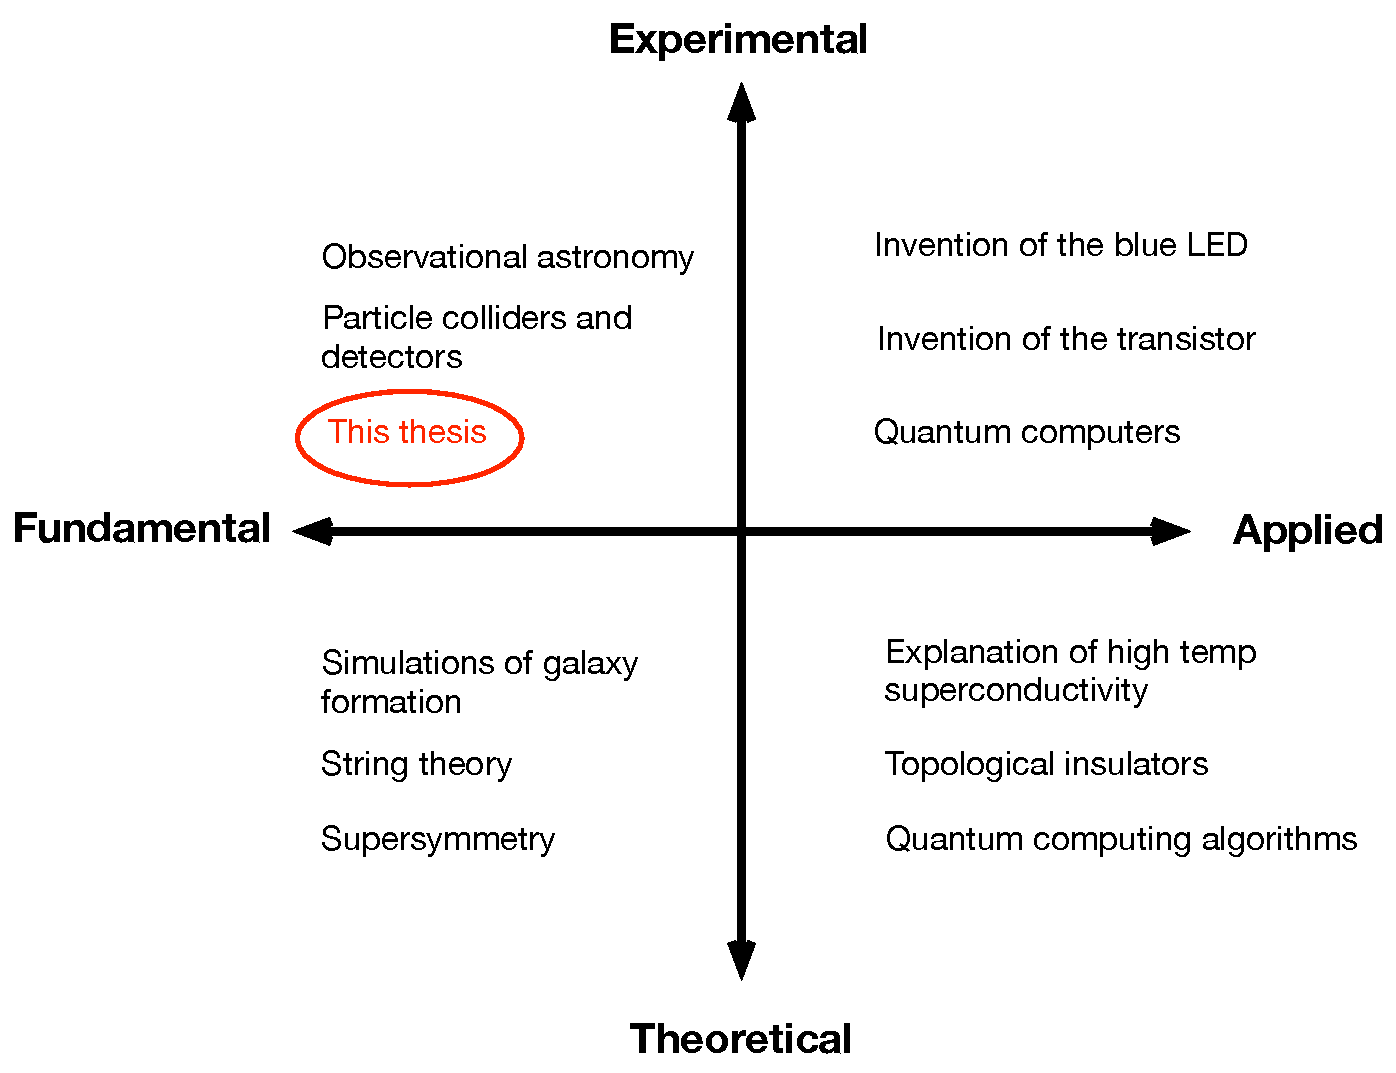
\includegraphics[width=6in]{cocktail_party_intro/types_of_physics_research.pdf}
\caption{A schematic diagram of physics research, from fundamental to applied, and experimental to theoretical, as well as several examples in each quadrant. Research topics often start in one quadrant and spread tentacles into others. Often, over time, fundamental research becomes more applied and theoretical research becomes more experimental, but sometimes the opposite happens, or neither. }
\label{fig:typesofphysicsresearch}
\end{figure}

To start to answer the \emph{Why?} of this thesis, let us consider the two fundamental quadrants. The fundamental--theoretical quadrant contains work like string theory and supersymmetry, and well as simulations designed to better elucidate the predictions of fundamental physics. This research often involves long calculations and heady math. Theorists often work in office complexes with endless supplies of white boards, and progress is made by thinking about a problem for a long time. Shoes aren't required, though many wear socks. Pencils are required, as well as the occasional computer to help evaluate the equations. To be sure, modern society would not exist without this quadrant. From Maxwell's electromagnetism to Einstein's relativity, what was originally fundamental theoretical became later became experimental and applied with the advent of radio, optical, and GPS technology. In other fields, such as quantum mechanics, fundamental theories and experiments developed in concert, but in all cases, the theoretical--fundamental understanding elucidated a crucial piece of the puzzle. 

Let's move on to the experimental--fundamental quadrant, which contains experimental work conducted to shed light on fundamental theories of nature. By fundamental I mean theories describing the building blocks of nature, or the fundamental properties of our universe. Sometimes the lines become blurry. Does chemistry belong here? Does biology? I would argue that because the understanding in these fields is largely empirical, and because they have yet to reach the point where a first principles approach is useful, these do not belong on our diagram of physics research. Astronomy is another difficult case, even as recently as a century ago astronomers, classification of galaxies into essentially arbitrary shape categories constituted a breakthrough. Over the twentieth century though, astronomy underwent a transformation into a field where practitioners observe astrophysical systems, test first principles-based theories or their behavior, and make quantitative predictions, to the point where many not refer to it as \emph{astrophysics}. Particle colliders are another example of research in this experimental--fundamental quadrant. 
 
Experimentalists build and use complex apparatuses to establish controlled conditions to test quantitative predictions of systems specifically sought out to study some fundamental property of nature. Many work in labs and shoes are nearly always required. We are lucky to have the generous support of institutions such as the Department of Energy, NASA, the National Science Foundation, as well as some private foundations to pursue this often expensive research which is almost always years, decades, or even centuries away from application.


\section[What is modern cosmology? \emph{Do you believe in the big bang?}]{What is modern cosmology?\\ \emph{\large{Do you believe in the big bang?}}}
%observational cosmology

The big bang is like biological evolution, the non-technical world makes a big fuss about it, but most scientists simply shake their heads and move on. Our understanding of biology and astronomy are so inextricably linked with these theories that there would practically be nothing left if we suddenly decided to reject them. A second point is that \textit{belief} not the most useful word here, or in science generally. To be sure, science requires at least a working belief that we live in a physical universe governed by mathematical laws, but if a scientific theory were backed up by so little data that it required \textit{belief} to be accepted, then it's unlikely to be very useful. There's an intermediate ground, of course, for theories in development or proposed before technology exists to test them, which no one would suggest discarding outright, but which aren't said to be ``accepted'' either. Rather, scientists say about string theory and supersymmetry, for instance, that the jury is still out.

In this section, I will discuss the modern field of cosmology and the evidence which puts the big bang squarely in the realm of fact. First, though, an important point about terminology. Many scientists and science popularizers play fast and loose with what the term `big bang' actually refers to. Does it refer to the predicted singularity 13.8 billion years ago when the whole observable universe fit on the head of a pin? Or both the singularity and its aftermath? Just its immediate aftermath, or the resulting expansion continuing into the present day? Or does it refer to the theory which predicts that that event? I suspect this ambiguity arises in part out of efforts to wow audiences at science lectures, and in part because the definition of the `big bang' is really beside the point in the technical literature. Experimentalists build instruments and study distant galaxies and theorists work to better understand the quantum field theory and general relativity. Editors don't make a big deal over the precise vocabulary used in paper introductions. Because of all this ambiguity, and because of the baggage the term `big bang' carries among the public, I prefer not to use it at all. Let's just discuss what we know.

I \textit{could} just describe our modern picture of the Galaxy, the universe and cosmology, but I fear it would be all to easy to simply dismiss it as a philosophy just like any other. So the purpose of this cocktail party introduction, I'll take a more historical approach and describe the main breakthroughs over the past century that have made cosmology the precision science that it is today. 

Our story begins in the early 1920s, by which time a number of poorly understood \textit{spiral nebulae}, fuzzy spiral blobs, had been observed in the night sky. There were essentially two possibilities. On the one hand, perhaps they were cloud of gas in the far reaches of our own galaxy; on the other, perhaps they were galaxies like our own but just farther away than object every seen before. The implications were enormous. Is there our galaxy all there is, or is it part of a space even more vast with countless others? Things came to a head in the famous Great Debate between astronomers Harlow Shapley and Heber Curtis at the Smithsonian in 1920 \citep{greatdebate}. The debate itself was mostly a stunt, scientific disputes aren't settled by debate but by better data. There were measurements that supported both points of view, but none of the data were extremely convincing. The dispute wasn't settled until Edwin Hubble, using the new 100\,in Palomar telescope on Mount Wilson, made the first measurements of the distances to these spiral nebulae, and demonstrated they were way outside our galaxy \citep{hubble26}. Hubble sought and monitored a type of pulsating stars in these nebulae called Cepheid variables, which are known to pulsate with a period proportional to their intrinsic brightness. Then by comparing their \textit{apparent} brightness, more distant objects generally appearing dimmer, their distances could be obtained. Many of the spiral nebulae were millions of light-years away, while our galaxy was known to be only about 50,000 light-years from side to side. The debate was settled, the universe was much larger than we had known.

For his next trick, Hubble turned his attention to even more distant galaxies, and the results were just as shocking. With only a few exceptions all appeared to be flying away from us at staggering velocities, hundreds or thousands of kilometers per second. Fast enough to travel around the earth in less than a minute. Moreover more distant galaxies were flying away from us faster, linearly faster. Exactly what you'd expect for a uniform expansion of space-time itself. It was as if a balloon with dots on it was being inflated; no matter which dot you're sitting on, all others are moving away from you at a rate proportional to their distance. I have reproduced Hubble's original data in Fig. \ref{fig:hubbleslaw}, which shows that the recession velocities a galaxy rises linearly with its distance. This relationship is known as Hubble's law, and the coefficient of proportionality, in units of velocity per distance, is knowns as the Hubble constant. Modern measurements place this value at roughly 70\,km/s/Mpc \citep{reiss16,planck16}, where 1\,Mpc = 1,000,000 parsecs. 

\begin{figure}
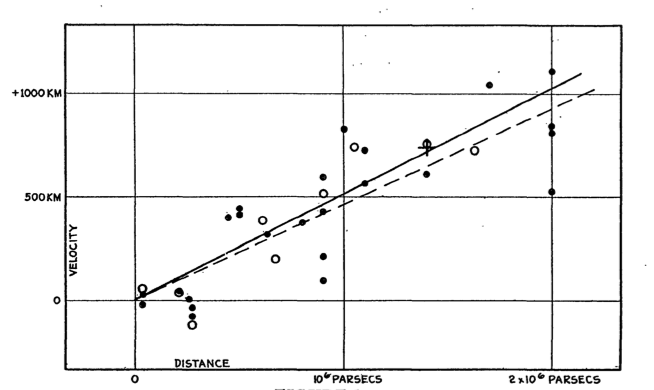
\includegraphics[width=6in]{cocktail_party_intro/hubble_diagram.png}
\caption{Hubble's measurements showed that galaxies in all directions are moving away from us at a speed linearly proportional to their distances. Here is his actual figure, reproduced from \citet{hubble29}, showing recession velocities of nearby galaxies in km/s (on the vertical axis) as a function of their distance from the Milky Way in parsecs (on the horizontal axis). Note 1 parsec is 3.26 light-years.}
\label{fig:hubbleslaw}
\end{figure}

How can the universe itself be expanding? What does that even mean? Einstein had applied the field equations of General Relativity to the universe as a whole and found that static solutions are impossible, which suggested to him that his equations were not completely correct. He found that a single constant added to the central field equation of the theory was sufficient to ensure a static solution, a \textit{cosmological constant} \citep{einstein17}. After hearing of Hubble's results, though, Einstein famously abandoned that addition, calling it his ``greatest mistake.'' It wasn't so much a \textit{mistake} per se, given that there wasn't any data at the time to test his prediction, more a missed opportunity. He could, after all, have gambled and \textit{predicted} the expansion of the Universe, and perhaps won a second Nobel prize for it.

Despite this early progress, cosmology was a research backwater for decades and for a time fell out of all memory, until the most unlikely creature of all, an engineer, made a breakthrough. In the course of developing ultra sensitive radio receivers at Bell Labs, Messrs. Anro Penzias and Robert Wilson were working with a horn antenna which seemed to pick up a very faint noise which they couldn't explain. 

Radio astronomers ofter quantify the power of radio emission by the equivalent temperature of a blackbody emitting the same amount of power. Let us build some intuition here, for a moment. Any object at a temperature $T$ emits electromagnetic radiation, the hotter it is, the higher frequency of the radiation. Objects at room temperature emit predominantly in the infrared band, while objects at a few thousand degrees, like the sun, emit in the optical band. At the other end of the spectrum, radio waves are emitted by very cold objects. Note of course that we are only talking about the  electromagnetic waves emitted by the random jostling around of atoms. By running currents through a wire, substantially more powerful radio waves may be produced which are not random at all, and are useful for transmitting Lady Gaga lyrics, among other things.

The background radiation detected by Penzias and Wilson was equivalent to that emitted by a very cold object, within a few degrees of absolute zero, 3 kelvin to be precise \citep{penzias65}. Moreover, it was the exact same brightness in any direction they looked away from our galaxy. Their discovery set off a flashbang in the cosmology community. Based on calculations of how nuclear fusion and fission calculations in a hot, dense early universe could account for the abundances of various stable and radioactive chemical elements, Ralph Alpher and Robert Herman calculated that the ambient temperature of empty space today to be roughly 5 kelvin \citep{alpher48,alpherherman,gamow48}.  The exact temperature was somewhat uncertain, and later estimates ranged from a few kelvin to tens of kelvin, but \citep{dicke65} immediately recognized that the observed 3 kelvin radiation was cosmic in origin, corresponding exactly to the aftermath of that hot, dense early state, what had been mocked as the `the big bang' by astronomers who opposed the theory. But much as it's a losing battle to keep non-scientists from referring the Higgs boson as `the God particle', the name `big bang' is not going anywhere soon. 

Two additional discoveries made in the early 1990s confirmed these results and set the stage for the more precise field of 21\,cm cosmology and the cosmic dawn that we address in this thesis. Both came from a satellite-born experiment named the Cosmic Background Explorer (COBE) designed to better study the cosmic microwave background discovered by Penzias and Wilson. The first key result was a precise measurement of its frequency spectrum. Man-made radiation or or experimental noise is rarely or never exactly thermal, that is, due only to random motions of atoms and electrons, and thus an exactly thermal spectrum is special. Radiation emitted by stars and galaxies ofter looks somewhat thermal, but atoms and dust inevitable emit or absorb some of it at different frequencies, always resulting in an imperfect frequency spectrum. In fact, the only known source of such a perfect thermal spectrum is the hot, dense early universe before galaxies had formed and everything was a sort of primordial soup, or more precisely, a purée. All scientific opposition to the hot, dense early universe model, ie, the `big bang' picture, evaporated after the publication of this spectrum, reproduced in Fig. \ref{fig:cobecmbspectrum}, published in \citep{cobespectrum,cobespectrum2}.

\begin{figure}
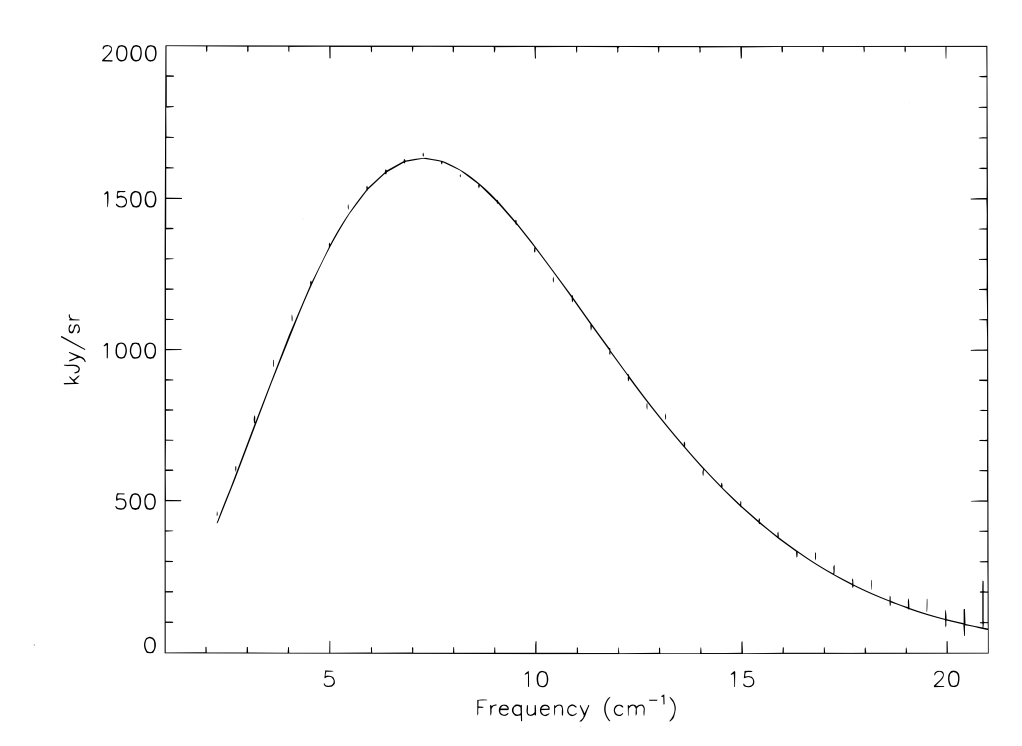
\includegraphics[width=6in]{cocktail_party_intro/cobe_cmb_spectrum.png}
\caption{CMB spectrum}
\label{fig:cobecmbspectrum}
\end{figure}


The second discovery was the icing on the cake. On top of clear evidence of the exotic hot, dense, homogenous early universe, COBE saw hints of how the modern \textit{clumpy} universe emerged. To the imprecise radio antenna of Penzias and Wilson, the cosmic microwave background appeared just as bright in every direction they looked. But the more sensitive COBE distinguished two interesting patterns. First, after subtracting the sky-averaged intensity corresponding to the 3 kelvin radiation, they observed a \textit{dipole} pattern in the sky. That is, the sky was uniformly brighter in one direction and fainter in the other, which was interpreted as the doppler shift of the cosmic microwave background due to the motion of our galaxy relative to other galaxies. It's as if our dot on the balloon is actually moving slowly across the balloon surface while the balloon is expanding, so dots on one side don't seem to be receeding as quickly, while those on the other appear to be receeding faster than they otherwise would. This \textit{anisotropy} of the cosmic microwave background shows us the slightly \textit{in}homogenieties in the nearly smooth early universe. 

\begin{figure}
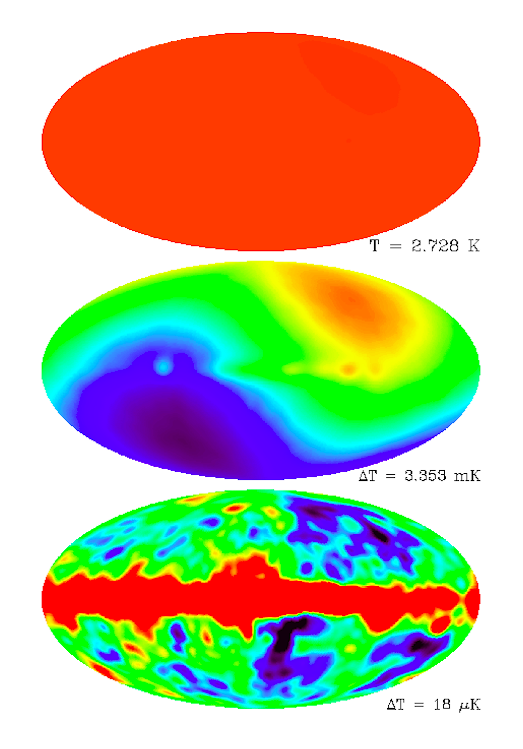
\includegraphics[width=6in]{cocktail_party_intro/cobe_cmb_anisotropy.png}
\caption{CMB anisotropy}
\label{fig:cobecmbanisotropy}
\end{figure}

Over time, we predict, but have yet to directly observe, that the denser regions slowly drew in more matter and collapsed due to gravitational attraction, eventually forming many galaxies. More recent CMB surveys by the WMAP \citep{wmap9year} and Planck \citep{planck15} satellites have confirmed and extended these results with exquisite precision, and truly made the past two decades the golden age of cosmology.


Lastly, I would be remiss if I didn't mention the most shocking discovery in cosmology over the past decades: the acceleration of the expansion of the universe. It does not directly relate to the work in this thesis, but it ties back to a thread discussed earlier. In 1997 and 1998, two groups attempting to reproduce, refine, and extend Hubble's original measurements (Fig. \ref{fig:hubbleslaw} to more distant galaxies, observed that galaxies a thousand times more distant that Hubble's appeared 
% 0.5 magnitudes is 10^(-0.5/2.5) = ~0.6
only half as bright as they should \citep{perlmutter97,riess08}. An obvious possibility is obscuration by dust, but both groups went to great lengths to demonstrate this was not the case. Dust absorbs preferentially red light, drastically altering the spectrum, but the spectra of these galaxies appeared normal. They were just fainter than their other properties suggested they should be. The consensus conclusion is that not only is the universe is expanding, but it is accelerating, due to exactly a term in Einstein's field equation like the cosmological constant he artificially added. But this time with living proof.

\section[What is the cosmic dawn? \emph{How did stars and galaxies form?}]{What is the cosmic dawn?\\ \emph{\large{How did stars and galaxies form?}}}
 
brief summary of the timeline of the universe, building on what we've learned in the previous section
nucleosynthesis, dark ages, cosmic dawn / reionization, modern universe / acceleration
highlight that CMB and dark galaxy surveys have closed in on the cosmic dawn, but it is the last major piece of the puzzle

why was the cosmic dawn an important and interesting epoch
pop III stars and reionization

pop III stars: what we know and don't know

reionization: what we know and don't know

the major problem: how do we study the universe before there were stars?

\section[21\,cm cosmology. \emph{How can we see into the darkness?}]{21\,cm cosmology\\ \emph{\large{How can we see into the darkness?}}}

solution to seeing into the epoch before stars: studying the faint radio emission from hydrogen gas
note: universe is 75\% hydrogen!
study evolution over time and space ==> tomography

hydrogen line and hyperfine transition
used in galactic astronomy to measure galactic rotation curve
intuitive physics of the hyperfine transition
1.4GHz line

redshifts to low frequency band
renaissance of low freq (100s of MHz) radio astronomy
how do interferometers work?
much cheaper than giant dishes, not possible with computing



%\chapter{Technical Introduction}

%%%%%%%%%%%%%%%%%%%%%%%%%%%%%%%%%%%%%%%%%%%%%%%%%%%%%%%%%%%%%%%%%%
\section{Observational cosmology: The state of the union}
%%%%%%%%%%%%%%%%%%%%%%%%%%%%%%%%%%%%%%%%%%%%%%%%%%%%%%%%%%%%%%%%%%

% paragraph 1
% what is the picture of the universe that has emerged over the past decades
% and how have these things been determined
Much like particle physics, cosmology today finds itself in the enviable yet frustrating position of having a broadly supported picture of the universe which leaves only the most challenging and fundamental questions  unanswered. Many intersecting lines of evidence point to a universe which began hot, dense, homogenous, and rapidly expanding 13.8 billion years ago, eventually cooled enough for bound objects to form, and is now accelerating. Studies of the Cosmic Microwave Background (CMB), high-z supernovae, distant galaxies, primordial element abundances, the matter power spectrum, and others all converge on this model. It is largely, however, a mal-understood and entirely unexpected \textit{dark} universe, whose total energy budget is dominated by constituents whose gravitational properties are well understood, but whose fundamental nature remains mystery. 

This universe is described by its energy densities of dark energy, $\Omega_\Lambda=0.691\pm0.006$, matter, $\Omega_M=0.309\pm0.006$, baryons, $\Omega_b=0.0455\pm0.0003$, and radiation, $\Omega_\gamma=(0.92\pm0.02)\times10^{-4}$. These densities are given as the present energy densities of these constituents relative to the present critical density $\rho_c=3H_0^2/8\pi G$, where the present expansion rate is $(70\pm2$)\,km/s/Mpc \footnote{I've estimated the uncertainty on $H_0$ as the approximate spread between the CMB measurement of $67.74\pm0.46$ km/s/Mpc and the local measurement of $73.2\pm1.7$}. Our universe is flat (ie, deviating from Euclidian geometry only due to a homogenous and isotropic expansion), with a measured curvature density of $\Omega_K=0.008\pm0.004$ which is consistent with zero. Further, the dark energy is consistent with being a cosmological constant, equivalent to a uniform vacuum energy, with an equation of state of $w=-1.02\pm0.08$, consistent with $-1$. These measurement represent the best combined constraints reported by \citet{planck16}, and have been made possible by the avalanche of data on the CMB, weak lensing statistics, baryon acoustic oscillations, and type 1a supernova surveys collected in recent years. 

Even with these precision measurements and the deluge of cosmology data, Joe Cosmologist has a sinking feeling at the pit of his stomach. Direct detection experiments for weakly interacting massive particles (WIMPs), the most natural dark matter candidate, have excluded essentially all reasonable parameter space for a particle freezing out at just the right time in the early universe to today's observed abundance. The easiest to swallow WIMP candidate was Supersymmetry's lightest, and thus stable, particle, the neutralino. But the mass scale of the supersymmetric partners was always a free parameter, and hopes of creating WIMPs at the Large Hadron Collider have been largely dashed. And dark energy is so challenging a problem that some some have even proposed it heralds the end of progress in the field \citep{darkenergybad}. 

Despite these questions, the general history of the universe is fairly well established. Nuclear reactions in the first few minutes of the universe created Hydrogen, Helium, Lithium, and trace amounts of XXX. Astronomers have verified these predictions of primordial abundances in XXX. After 370,000 years of expansion and cooling, the photon mean free path increased to larger than the Hubble radius and protons and neutrons formed into atoms. That photon bath still permeates the universe as the CMB, and its anisotropies represent order $10^-5$ density and temperature fluctuations at recombination. After the release of the CMB, before sources formed, those slight fluctuations began to collapse under gravity during a period known as the dark ages. After a few hundred million years, sufficient densities and temperatures were reached in these collapsing halos to form the first bright sources in a period known as the cosmic dawn, culminating in the epoch of reionization. These bright sources are thought to have irradiated the IGM with ionizing photons, reionizing the formerly neutral Hydrogen. The deepest galaxy surveys reach barely reach back to this epoch, detecting only a handful of the rarest and brightest galaxies, leaving mysterious the general characteristics of the cosmic dawn.

Many questions remain about this first generation of sources. How big were they? How bright? How numerous? Were they stars? Black-hole binaries? Quasars? NEED SOME OTHER QUESTIONS TO POSE HERE

After this epoch, though, our knowledge becomes firmer. Observations of the Lyman alpha forest in quasar sightlines have revealed the reionization of the universe progressing from small bubbles into the whole volume. Galaxy redshift surveys have confirmed predicted statistics of the matter distribution at essentially all but galactic scales, and numerical simulations are beginning to nail down the complex astrophysics of galaxy formation.

New generations of observatories are coming on in the coming years to tackle all these problems, at the very least by drowning us in data. LSST will survey the sky every night, discovering tens of thousands of supernova to characterize the acceleration to unprecedented precision. Redshift surveys like WFIRST and EUCLID will measure millions of galaxy redshifts to trace the statistics of structure over time, and the James Webb Space Telescope will probe deeper into the EOR in just hours than Hubble probed in XX days. (IS THAT RIGHT???). Perhaps in more ways than one, we are on the verge of first light.

%%%%%%%%%%%%%%%%%%%%%%%%%%%%%%%%%%%%%%%%%%%%%%%%%%%%%%%%%%%%%%%%%%
\section{Closing in on the cosmic dawn}
%%%%%%%%%%%%%%%%%%%%%%%%%%%%%%%%%%%%%%%%%%%%%%%%%%%%%%%%%%%%%%%%%%

In our history of the universe, the clear gap in observations is the cosmic dawn. In this section we go into detail into what is known about this epoch from indirect measurements and what uncertainties remain.

% paragraph 6
% closing in from high z
CMB and numerical simulations closing in from high z side
CMB optical depth
post CMB universe is neutral and homogenous

% paragraph 7
% closing in from low z
deep galaxy surveys (HUDF)
present universe is ionized, and clumpy
gunn-peterson trough
some conflicting constraints with high z (tau)

% paragraph 8
% simulating the EOR
astrophysics of reionization / feedback effects 

% paragraph 9
% first sources
pop III stars
low energy SNe (cite Alex Ji's paper)


%%%%%%%%%%%%%%%%%%%%%%%%%%%%%%%%%%%%%%%%%%%%%%%%%%%%%%%%%%%%%%%%%%
\section{21cm tomography}
%%%%%%%%%%%%%%%%%%%%%%%%%%%%%%%%%%%%%%%%%%%%%%%%%%%%%%%%%%%%%%%%%%%

% paragraph 10
% basic idea
detect 21cm emission from neutral hydrogen during the EOR
negative images of the growing ionized bubbles around galaxies

% paragraph 11
% 21cm emission
few words about history
	first spectral line identified for radio astronomy (van der Hulst and Oort)
	rotation curve measurements of the galaxy => dark matter halo
physics of the hyperfine transition \citep{griffithshyperfine}

% paragraph 12
% 21cm from the EOR
Consider a radiation field with intensity $I_0$ behind a cloud of Hydrogen with optical depth $\tau$. The emergent intensity is $I_\nu=I_0e^{-\tau}+S_\nu(1-e^{-\tau})$. Cosmological redshift reduces the observed energy flux by $(1+z)$, then formulating in terms of brightness temperatures and assuming $\tau<<1$ gives:

\begin{equation}
\delta T=\frac{T_s-T_\gamma(z)}{1+z}
\end{equation}
where $T_s$ is the brightness temperature of 21cm radiation from the gas, equal to the spin temperature of the gas. This can be proved using $S_\nu=j_\nu/\alpha_\nu\propto A n_2/(n_1B_{12}-n_2B_{21})=\nu^2 T_s$, where the last equality uses $A\sim\nu^3B$, which is the rayleigh jeans relation with the spin temperature. Now we just need the optical depth through the cloud with size $ds$.

\begin{equation}
\tau=\int\alpha ds=\int\frac{h\nu}{c}\phi(\Delta\nu)(n_1B_{12}-n_2B_{21})ds
\end{equation}
Then using $g_1B_{12}=g_2B_{21}$, $g_2/g_1=3$, and $n_2/n_1=3e^{-h\nu/kT_s}$ gives

\begin{equation}
\tau=\int\frac{h\nu}{c}\phi(\Delta\nu)\frac{n_H}{4}B_{12}(1-e^{-h\nu/kT_s})ds
\end{equation}
using $n_H=n_1/4$, given that $T_s>>h\nu/k=0.1$K. Recall that $B$ has units of $A$ divided by energy density per frequency, giving $A\sim Bh\nu^3/c^3$, and to be precise there is an $8\pi$ here. Also taylor expand the exponential:

\begin{equation}
\tau=\phi(\Delta\nu)\frac{n_H}{4}\frac{Ac^2}{8\pi\nu}\frac{h}{kT_s}\Delta s
\end{equation}
Now use that photons travel on geodesics so we may replace $\Delta s=a(t)\Delta r$ by $c\Delta t=c\Delta z/(1+z)H(z)$, and also use that the line is doppler broadened by $\Delta\nu/\nu=v/c=H(z)\Delta s/c$, with $\phi(\Delta\nu)=1/\Delta \nu$, giving:
\begin{equation}
\tau=\frac{n_H}{4}\frac{Ac^2}{\nu}\frac{h}{8\pi kT}\frac{c}{H(z)\nu}
\end{equation}

\begin{equation}
\tau=\frac{T_s-T_\gamma(z)}{1+z}\frac{\Omega_b\rho_c(1+z)^3}{4}\frac{Ac^2}{8\pi\nu}\frac{h}{kT_s}\frac{c}{H_0\sqrt{\Omega_m}(1+z)^{3/2}\nu}
\end{equation}

\begin{eqnarray}
\delta T&=&\sqrt{1+z}\left(1-\frac{T_\gamma(z)}{T_s}\right)\frac{\Omega_b}{4}\frac{3H_0}{8\pi Gm_p}\frac{h}{8\pi k}\frac{c}{\sqrt{\Omega_m}}\left(\frac{c^2A}{\nu^2}\right)\\
&=&10\text{mK}\left(\frac{1+z}{10}\right)^{1/2}\left(1-\frac{T_\gamma(z)}{T_s}\right)
\end{eqnarray}
where $T_s>>T_\gamma$ during reionization. 

% the global signal
As we see above, the brightness temperature of the 21cm signal is determined by the spin temperature. That temperature is affected by three processes: collisional coupling with atoms and free electrons which couple the gas kinetic temperature to the spin temperature, radiative coupling to the CMB, and Ly$\alpha$-induced spin-flips via an excited state. 

\textbf{$1100>z>200$} The universe is dense enough so that collisional coupling between atoms and residual free electrons holds $T_\text{gas}=T_\gamma=T_s$, and $\delta T=0$.

\textbf{$200>z>50$} Now the gas is cooling adiabatically with $PV^\gamma=$const, with $\gamma=c_p/c_v=1+1/c_v$, and $c_v=f/2$. Note also that $TV^{\gamma-1}=$const, giving that $T\sim (1+z)^2$ for $f=3$ for a monotonic ideal gas. So the gas cools below the CMB temperature, and the spin temperature is still coupled to the gas temperature. Thus 21cm signal is now visible in absorption. This is the pristine cosmological signal, and is the long run focus of 21cm cosmology.

\textbf{$50>z>z_\text{re}$} This is the epoch of heating at reionization, and the exact sequence of events is quite uncertain. The spin temperature gets heated far above the CMB temperature by the first luminous sources. 21cm fluctuations are sourced by some combinations of Ly$\alpha$ flux, density fluctuations, and neutral fraction fluctuations.  

\textbf{$z_\text{re}>z$} Most of the universe is ionized, and 21cm signal is now only visible in large scale 21cm overdensities. 


% paragraph 13
% tomography
low optical depth (ie, long lifetime, very weak transition) spectral line ==> tomography!!
redshift corresponds to line of sight distance
and angle corresponds to transverse distance

% paragraph 14
% a problem: foregrounds
extragalactic sources
galactic synchrotron
huge thermal noise 


%%%%%%%%%%%%%%%%%%%%%%%%%%%%%%%%%%%%%%%%%%%%%%%%%%%%%%%%%%%%%%%%%%
\section{The radio interferometry renaissance}
%%%%%%%%%%%%%%%%%%%%%%%%%%%%%%%%%%%%%%%%%%%%%%%%%%%%%%%%%%%%%%%%%%

% paragraph 15
% what types of instruments are needed to detect the faint signal
first generation instruments : power spectrum measurements
related to the matter power spectrum
targeted to ultra low surface brightness emission ==> compact arrays
large N / small D (with advances in computing power, large dipole arrays)

% paragraph 16
% power spectrum measurements with interferometers
physics of radio interferometry (van der cittert-zernike theorem)
relating visibilities to power spectr

% paragraph 17
% global signal measurements
EDGES (lower limit on EOR duration)

% paragraph 18
% first generation interferometers
MWA
PAPER
	power spectrum expts (lower limit on the EOR spin temp)
GMRT

% paragraph 19
% challenges
calibration => omniscape
antenna characterization
deconvolution and surveys (Patti and Jack's work, Danny's 2013 paper)
faint RFI flagging

% paragraph 20
% next generation interferometers
HERA happening now
SKA happing over the next decade


%%%%%%%%%%%%%%%%%%%%%%%%%%%%%%%%%%%%%%%%%%%%%%%%%%%%%%%%%%%%%%%%%%
\section{Completing the picture with cross correlations}
%%%%%%%%%%%%%%%%%%%%%%%%%%%%%%%%%%%%%%%%%%%%%%%%%%%%%%%%%%%%%%%%%%

% paragraph 21
% basics of why xcors will help
confirming any detections
	systematics are pernicious
	more sensitive radio interferometry than every before
extending the science
	IGM connects to stellar properties, connects to galaxy surveys

% paragraph 22
% 21cm/optical
Tzu-Ching
Beardsley (adding context to JWST)

% paragraph 23
% 21cm/Ly-alpha
brief intro to my project


\chapter{Introduction}


\section{Cosmology and the cosmic dawn}

\subsection{Modern cosmology and the history of the universe}

Much like particle physics, cosmology today finds itself in the enviable yet frustrating position of having a broadly supported picture of the universe with only the most challenging and fundamental questions unanswered. Many intersecting lines of evidence point to a universe which began hot, dense, homogenous, and rapidly expanding 13.8 billion years ago, eventually cooled enough for bound objects to form, and is now accelerating. Studies of the Cosmic Microwave Background (CMB), high-z supernovae, distant galaxies, primordial element abundances, the matter power spectrum, and other observables all converge on this model. It is largely, however, a mal-understood and entirely unexpected \textit{dark} universe, whose total energy budget is dominated by constituents whose gravitational properties are well understood, but whose fundamental nature remains mysterious. 

The simplest (i.e., \textit{vanilla}) model which agrees with all available data is parameterized by the energy densities of baryons ($\Omega_b=0.0455\pm0.0003$), cold dark matter  ($\Omega_m=0.3089\pm0.0062$), and vacuum energy ($\Omega_\Lambda=0.69\pm0.0062$), the amplitude ($\ln (10^{10}A_s)=3.064\pm0.023$) and spectral index ($n_s=0.9667\pm0.004$) of the primordial power spectrum, and the optical depth to reionization ($0.066\pm0.012$). 
The energy densities are given as the present densities of these constituents relative to the present critical density $\rho_c=3H_0^2/8\pi G$, where the present expansion rate is $(70\pm3$)\,km/s/Mpc
\footnote{I've taken the uncertainty on $H_0$ to be the spread between the CMB measurement of $67.74\pm0.46$ km/s/Mpc \citep{planck16} and the local measurement of $73.2\pm1.7$ \citep{reiss16}.}. 
On scales larger than hundreds of Mpc, our universe is flat, deviating from Euclidian geometry only due to a homogenous and isotropic expansion, with a measured curvature density consistent with zero of $\Omega_K=0.008\pm0.004$. 
Further, the equation of state of dark energy is constrained to be $w=-1.02\pm0.08$, consistent with -1, and thus, with a true cosmological constant or a uniform vacuum energy. These measurements represent the best combined constraints reported by \citet{planck16}, and have been made possible by the avalanche of data on the CMB, weak lensing statistics, baryon acoustic oscillations, and type 1a supernova surveys collected in recent years. 

In this framework, the history of the universe is fairly well established. Nuclear reactions in the first few minutes of the universe created Hydrogen, Helium, Lithium, and trace amounts of deuterium and lithium, and astronomers have verified these predictions of primordial abundances to high precision \citep{bbn}. After 370,000 years of expansion and cooling, the photon mean free path increased to larger than the Hubble radius and protons and neutrons formed atoms. The CMB is that relic photon gas, and its anisotropies represent order $10^-5$ density and temperature fluctuations at recombination. After the release of the CMB, before sources formed, those slight fluctuations began to collapse under gravity during a period known as the dark ages. After a few hundred million years, sufficient densities and temperatures were reached in these collapsing halos to form the first bright sources in a period known as the cosmic dawn, culminating in the epoch of reionization. 

The basic sequence of events is well understood. These very massive and bright stars (known as Population III stars) formed from primordial (metal-free\footnote{Note that in astronomy nomenclature, all atoms heavier than Helium are known as \text{metals}.}) gas are thought to have irradiated the IGM with ionizing photons, reionizing the formerly neutral intergalactic medium. Nucleosynthesis processes in their supernova are thought to have polluted galaxies with the metals needed for gas to more easily collapse and cool, allowing modern stars to form. 

Many questions remain about this first generation of sources. How massive were they? How bright? How numerous? What were the relative contributions of stars, black hole binaries, and quasars? When exactly did these first stars form and how long did it take? How many linger in stellar halos? Simple n-body simulations can model the gravitational collapse of the cosmic web and dark matter halos, but complex feedback and subgrid physics models are needed to understand the the baryonic processes involved in the formation of stars and galaxies. It is no wonder progress has been slow, these stars and galaxies are by definition the farthest and faintest ones that can ever hope to observe, and understanding their formation, before any stars even shone at all, is even more of a challenge. 

This thesis presents experimental work in the field of 21\,cm cosmology, a promising avenue to circumvent the catch-22 of how to study galaxies before they began to emit light. The idea, which I discuss in detail in Sec. \ref{sec:intro21cmsection}, is to study not the galaxies themselves, but instead the intergalactic medium between them. In particular, we seek to measure the slight low frequency radio emission from the neutral hydrogen between galaxies in order to map out the matter distribution of the universe, and then once stars begin to form and irradiate this neutral gas, observe the resulting ionized bubbles growing around galaxies over cosmic time. 

Eventually the whole volume of the intergalactic medium is ionized, and this last phase transition of the universe is known as the Epoch of Reionization, thought to have occurred in the first few hundred million years of the universe ($6\lesssim z\lesssim12$), following the Dark Ages ($20\lesssim z\lesssim 1100$) when gravitational collapse assembled the galaxies themselves. Broadly, the study of the formation and evolution of these first stars and galaxies is known as the Cosmic Dawn, and it is the missing link between the hot, smooth post-big bang universe and the modern clumpy universe we know today.


\subsection{Reaching towards the cosmic dawn}

For all the questions about the astrophysics of reionization and the lack of direct observations, a number of indirect constraints establish a rough picture of the EOR and bound its beginning and end. 

% Ly-alpha forest
The Lyman alpha forest and its transformation into Gunn-Peterson trough at $z\sim6$ provide perhaps the clearest evidence of the evolving ionized fraction of the IGM. Quasars are an observational category of active galaxies whose smooth spectrum jets happen to be oriented along our line of sight. At redshifts $1<z<3$ the band between Lyman continuum and Lyman alpha becomes increasingly crowded with absorption lines, indicating that these quasar beams have traversed more and more neutral hydrogen clouds at intermediate redshifts. Between $3<z<5$, these lines become so crowded, that there is no apparent continuum level, and at higher redshifts close to the end of reionization, there are enough neutral hydrogen atoms left everywhere that all emission in this band is absorbed. A caveat is that the Lyman alpha line saturates at even very small neutral fractions down to $\sim10^{-5}$ \citep{FurlanettoReview}, so the appearance of a Gunn-Peterson trough is evidence only of the tail end of reionization. The mid point and indeed the whole reionization history is unconstrained by these observations.

SHOW THE GRAPHIC THAT TOM IS MAKING FOR ME

% CMB optical depth measurements
An orthogonal constraint on the redshift of reionization derives from the measurement of the thompson scattering optical depth $\tau$ between us and recombination. Scattering of CMB photons off free electrons tends to smear out the temperature anisotropies, damping the power on all angular scales scales as $e^{-2\tau}$, however there are no free electrons in the intergalactic medium immediately after recombination. Such scattering does not occur until the epoch of reionization, when the first sources irradiate the neutral IGM, sourcing free electrons which scatter CMB photons. The optical depth to the CMB is thus a measure of how much ionized medium the CMB must propagate up until today. Assuming reionization occurred instantaneously at $z_\text{re}$, the thompson scattering optical depth is 
\begin{equation}
\label{eqn:opticaldepthcmb}
	\tau=\int n_e\sigma_t ds=\sigma_t c\int_0^{z_{re}}\frac{dz}{H(z)(1+z)}\frac{\Omega_M(1+z)^3\rho_c}{m_p}
\end{equation}
where $n_e$ is the number density of free electrons, $\sigma_t$ is the thompson scattering optical depth, $\rho_c=3H_0^2/8\pi G$ is the present critical density of the universe, and $m_p$ is the proton mass. Recent constraints by \citep{plancktau16} give roughly $\tau=0.06\pm0.01$, depending on the priors used and which other constraints are included, implying a reionization redshift of $z_{re}=9\pm1$ using Eqn. \ref{eqn:opticaldepthcmb}.

This is far from the end of the story, though. Reionization did not occur instantaneously, and the detailed evolution of the ionized fraction over redshift will affect this calculation. In fact \citet{bowman2010} set a lower limit of $\Delta z>0.06$ (95\%) based on lack of an abrupt step in the 21\,cm global signal over redshift (i.e., frequency). Further, the optical depth is somewhat degenerate with the amplitude $A$ of the primordial power spectrum on all but the large angular scales. There is a large angular scale peak in the E model polarization power spectrum due to the proximity of ionized bubbles to us, but both large scale effects are limited by cosmic variance uncertainties. Constraints on the midpoint and duration of reionization would go a long way to pinning down the astrophysics of the EOR \citep{liu15a}.

% deep galaxy surveys (photometry) (Hubble and JWST)
Deep galaxy surveys and cluster lensing surveys are finding tens of EOR galaxies at $6<z<10$ \citep{Bouwens2011,Illingworth2013,Dunlop2013}, probing down to $M_{AB}sim-17$. See the review by \citet{madau14review} Note that these high-$z$ galaxies are properly referred to as \textit{candidates} though, as their redshifts are estimated photometrically and they are too faint for spectroscopy. Such observations directly probe the UV luminosity function, which, after assuming an escape fraction and faint end slope, yields estimates of the reionization history. \citet{RobertsonReionization2015} then calculate the implied optical depth to the CMB and find reasonable agreement with the latest $\tau$ results from Planck analyses, in contrast to earlier Planck \citep{Robertson2013} and WMAP \citep{hinshaw_et_al_2012} results. Still, the error bars are large and JWST will be needed to probe down to the $M_{AB}\sim-13$ galaxies thought to generate the bulk of ionizing photon flux.

Cross correlation experiments comparing these EOR galaxies with 21\,cm observations should provide an important cross check on these results, though the mismatched resolutions pose a problem. The full Hubble deep field with its hundreds of high redshift galaxies fits easily inside a single MWA resolution element. One possible solution to compare the galaxies found in 21\,cm bright spots with those found in 21\,cm dark spots, as the former should be more characteristic of the ionizing population \citep{beardsley15}, and in Ch. \ref{chap:xcor} I discuss ways to realize an intensity mapping correlation without having to detect individual sources in either map.

Other probes are also beginning to bring the EOR into focus, but many require significant assumptions or empirical fitting to relate their predictions to the EOR. Stellar archeology is the study of the oldest, most metal poor (Population II) stars in our own galaxy. These stars formed from gas enriched by only a few supernovae events, and their chemical abundances constrain the properties of the supernovae of first generation stars (Population III), which will eventually allow us to constrain the properties of these first stars \citep{Frebel2015}. Further, n-body simulations can shed light on the mass and luminosity function of the first galaxies and reionization, albeit after incorporating empirically motivated models of complex astrophysical feedback \citep{Bauer2015,Vogelsberger2014} . Lastly, semi-numerical EOR simulations like 21cmFAST \citep{21cmfast} parameterize the EOR with a small number of astrophysical parameters, simplifying the extraction of astrophysical constraints from 21\,cm observations \citep{PoberNextGen,PoberPAPER64Heating}. 

For all we have pieced together, it is worth emphasizing that many questions remain unanswered. Which galaxies generated the bulk of ionizing photons, and what fraction of their photons reached the IGM? What were the masses and luminosities of Population III stars, when did they form, and what did their supernovae look like? What role did pre-reionization sources like black hole binaries and AGN feedback play in heating the intergalactic medium. And eventually, can we understand and model all this \textit{gastrophysics} to get at the matter power spectrum of the universe, and from there, constrain the underlying cosmology?

\section{Theory of 21cm tomography}
\label{sec:intro21cmsection}

\subsection{Radio emission from neutral hydrogen}

A standard result of quantum mechanics \citep[e.g.,][]{griffithsqm} is that, to first order, the energy levels of the Hydrogen atom are $E_n\approx13.6\,\text{eV}/n^2$, where $n=1,2,3,...$. Each state corresponds to a solution to the Schrodinger equation describing an electron bound to a proton, neglecting their finite sizes, intrinsic spins, and relativistic effects. At thermal equilibrium, statistical mechanics predicts the relative fraction of atoms in the $n$'th state is given by the Boltzmann factor $e^{-E_n/kT}$, so that typically only low integer states are populated, and transitions between them release the energy differences as ultraviolet, optical, or near infrared photons. 

At higher order, relativistic effects shift the energy levels, and the coupling of the electron's spin and orbital angular momentum split each $n$ state into several $\ell$ states. The sum of these effects is known is Hydrogen fine structure, though as the ground state has no orbital angular momentum, it is not split at this order. 

\begin{figure}
	\centering
	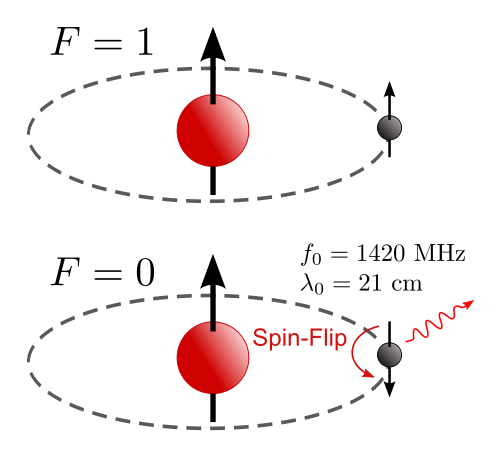
\includegraphics[width=4in]{chap0_intro/500px-Hydrogen-SpinFlip.svg.png}
	\caption[Diagram of the two Hydrogen ground states resulting from hyperfine splitting.]{Typical visualization of the two Hydrogen ground states resulting from the hyperfine splitting \citep{HydrogenSpinFlipGraphic}, where $F$ is the total angular momentum of the system, and the transition between the two states results in emission of a 21\,cm photon.}
	\label{fig:HydrogenSpinFlipGraphic}
\end{figure}

Finally, at higher order, the coupling of the proton and electron spins splits all states into those where the electron and proton spins are parallel, and those where they are antiparallel, as in Fig. \ref{fig:HydrogenSpinFlipGraphic}. The energy difference is much smaller than the differences between the $n=1,2,3$ states, and corresponds to emission or absorption of a low frequency radio photon with wavelength 21\,cm. In the upper (lower) state the spins are parallel (anti-parallel). Note that this disagrees with classical intuition, as when the spins are parallel, the magnetic dipole moments are antiparallel, and just as two antialigned magnets tend to attract, this state should actually have \textit{lower} energy. 

In response, is often remarked simply that quantum mechanics sometimes makes counterintuitive predictions, though \citet{griffiths82} argues that there is a more intuitive way to understand the situation. He observes that Fig. \ref{fig:HydrogenSpinFlipGraphic} misleadingly suggests that the electron is displaced from the proton, when in fact its spherical wavefunction encompasses it, and thus it is more correct to picture their magnetic moments as tiny current loops in the $xy$ plane (perpendicular to the proton spin). If both spins are aligned, then the current loops flow in opposite directions, and thus repel just like parallel wires with opposite currents, explaining which this is the higher energy state.

Lastly, note that in the upper state when the spins point in the same direction, the quantization of $z$ angular momentum makes this actually a spin triplet state, so there are three upper states and one lower state.

\subsection{21cm emission from the Dark Ages and Epoch of Reionization}

In this section I review theoretical calculacions of the observed 21\,cm brightness temperature of a neutral cloud in the intergalactic medium (IGM) during the Epoch of Reionization (EOR), mainly following \citet{PritchardLoebReview}, but filling in many missing details and background information where helpful. 

\subsubsection{Microscopic radiative transfer using Einstein A and B coefficients}

The Hydrogen atom is not a simple quantum mechanical system, and even less so taking into account fine and hyperfine structure, but fortunately in the cool, dilute intergalactic medium, the problem simplifies greatly. Essentially all hydrogen atoms are in the ground state at temperatures  $T<<10\text{eV}/k_B\sim10^5$K, which is always the case before the EOR when gas temperatures are $10-100$\,K, and after the EOR when they are $100-1000$\,K \citep{FurlanettoReview}. Thus only the hyperfine states are allowed, and we may regard such atoms at two level systems with an energy spacing of $\Delta E=hc/\lambda\approx6\mu$\,eV, where $\lambda=21$\,cm, and there is a three-fold degeneracy of the upper state. The four states are roughly equally populated as $T>>\Delta E/k_B =0.06$K, giving number densities of excited ($n=2$) and ground ($n=1$) state atoms as $n_2=\frac{3}{4}n_H$, and $n_1=\frac{1}{4}n_H$, where $n_H$ is the overall density of hydrogen atoms. Note that this $n=1,2$ indexes only the two hyperfine states, it is not the general $n$ used above to index all the energy levels of hydrogen. Lastly, note that the spontaneous emission lifetime of the upper excited state is roughly $10^7$\,years.

Before considering radiative transfer through the universe of 21\,cm emission from a hydrogen cloud at high redshift, we first comment on the different parts of this non-thermodynamic equilibrium problem, and present the Einstein A and B coefficients we will use to treat them. The three temperatures in this problem are: (1) the hydrogen gas temperature, encodinge the root mean square velocities of the particles; (2), the spin temperature, defined as the temperature of an ensemble of two level atoms having the same ratio of excited to ground state atoms as our system; and (3) the temperature of the cosmic microwave background, a blackbody radiation field which backlights our neutral hydrogen clouds during the EOR. 

Our task is to calculate the emergent intensity through an HI cloud with optical depth $\tau$ backlit by the CMB. From standard radiative transfer theory, the answer is $I_\nu=I_0e^{-\tau}+S_\nu(1-e^{-\tau})$, however because our three temperatures are not the same, the source function $S_\nu\equiv j_\nu/\alpha_\nu$ does not in general equal a planck (i.e., blackbody) function\footnote{The planck function is given by $B_\nu(T)\propto\nu^3/(e^{h\nu/kT}-1)$} and we thus require a microscopic description of the radiation field using the Einstein A and B coefficients.

Consider again our two level atom with number densities $n_2$ and $n_1$ in the excited and ground states, respectively. The Einstein coefficients are defined by:
\begin{eqnarray}
\text{\# spontaneous emissions per volume per time}&=&An_2 \nonumber\\
\text{\# stimulated emissions per volume per time}&=&B_{21}n_2u_\nu \nonumber\\
\text{\# absorptions per volume per time}&=&B_{12}n_1u_\nu 
\end{eqnarray}
where $u_\nu$ is the energy density per frequency of the radiation field. Note that $A$ has units of $\text{s}^{-1}$, and the $B$'s have units of $\text{s}^{-1}(\text{energy density per frequency})^{-1}$. We can construct the unit of energy density per frequency as $h\nu/(c/\nu)^3/\nu$, thus on purely dimensional grounds we expect $A\approx B (h\nu^3/c^3)$, which is the correct relation from atomic physics up to a factor of $8\pi$. Einstein showed that $g_1B_{12}=g_2B_{21}$ (where in our case $g_1=1$, $g_2=3$) regardless of whether the atoms are in thermal equilibrium with the radiation field.

Before calculating the radiation source function, let us look at the radiative transfer equation to understand how to treat stimulated emission,
\begin{equation}
\frac{dI_\nu}{ds}=j_\nu-\alpha_\nu I_\nu
\end{equation}
where $I_\nu$ is the specific intensity, with units of energy per area per solid angle per frequency per time. As the stimulated emission rate is proportional to the radiation density it makes sense to think of it contributing \textit{negatively} to the absorption coefficient. So the emission coefficient is due solely to spontaneous emission, and has units of energy per volume per time per solid angle per frequency. Integrating over the spectral line, the energy emitted per volume per time per solid angle is:
\begin{equation}
\int j_\nu d\nu=\frac{1}{4\pi}h\nu n_2 A
\end{equation}
If we introduce a line shape $\phi(\nu-\nu_0)$ with $\int\phi(\nu-\nu_0)=1$, where $\nu_0$ is the center frequency of the spectral line, then we have:
\begin{equation}
\boxed{j_\nu=\frac{h\nu_0 n_2A\phi(\nu-\nu_0)}{4\pi}}
\end{equation}

Now consider a beam with intensity $I_\nu$ passing through the atoms. The energy density in the beam is $u_\nu=I_\nu/c$, so the energy absorbed from the beam per volume per time is $\int d\nu\int d\Omega\alpha_\nu I_\nu$, which can also be expressed as $\int d\nu h\nu_0\phi(\nu-\nu_0)(n_1B_{12}-n_2B_{21})I_\nu/c$, which gives:
\begin{equation}
\boxed{\alpha_\nu=\frac{h\nu_0\phi(\nu-\nu_0)(n_1B_{12}-n_2B_{21})}{c}}
\end{equation}

Then the source function is
\begin{equation}
\boxed{S_\nu=\frac{4}{4\pi}\frac{ n_2A}{n_1B_{12}-n_2B_{21}}}
\end{equation}
which is valid even if the atoms are not in thermodynamic equilibrium with the radiation field. 

\subsubsection{Brightness temperature of an HI cloud in the EOR}

Now let us put the pieces of this calculation together and relate them to the observed emergent intensity of the CMB shining through an HI cloud during the EOR. As above, considering a radiation field with intensity $I_0$ behind a cloud of Hydrogen with optical depth $\tau$, the emergent intensity is $I_\nu=I_0e^{-\tau}+S_\nu(1-e^{-\tau})$. Cosmological redshift reduces the observed energy flux by $(1+z)$, and then reformulating the equation in terms of brightness temperatures and assuming $\tau<<1$ (because this is a very weak transition) gives
\begin{equation}
\delta T=\frac{T_s-T_\gamma(z)}{1+z}\tau 
\end{equation}
where $T_s$ is the brightness temperature of 21\,cm radiation from the gas, equal to the spin temperature of the gas\footnote{We can prove that the spin temperature equals the brightness temperature of the gas noting that $S_\nu=j_\nu/\alpha_\nu\propto A n_2/(n_1B_{12}-n_2B_{21})\propto\nu^3n_2/(3n_1-n_2/n_1)\approx\nu^2 T_s$, which is the rayleigh jeans relation with the spin temperature instead of the typical gas temperature. Note that we have used  $A\propto\nu^3B$ and $n_2/n_1\equiv3e^{-h\nu/kT_s}\approx3(1-h\nu/kT_s)$}. Now we just need the optical depth through the cloud with size $ds$.

\begin{equation}
\tau=\int\alpha ds=\int\frac{h\nu}{c}\phi(\Delta\nu)(n_1B_{12}-n_2B_{21})ds
\end{equation}
Then using $g_1B_{12}=g_2B_{21}$, $g_2/g_1=3$, and $n_2/n_1=3e^{-h\nu/kT_s}$ gives

\begin{equation}
\tau=\int\frac{h\nu}{c}\phi(\Delta\nu)\frac{n_H}{4}B_{12}(1-e^{-h\nu/kT_s})ds
\end{equation}
using $n_H=n_1/4$, given that $T_s>>h\nu/k=0.1$K. Recall that $B$ has units of $A$ divided by energy density per frequency, giving $A\sim Bh\nu^3/c^3$, and to be precise there is an $8\pi$ here. Also taylor expand the exponential:

\begin{equation}
\tau=\phi(\Delta\nu)\frac{n_H}{4}\frac{Ac^2}{8\pi\nu}\frac{h}{kT_s}\Delta s
\end{equation}
Now use that photons travel on geodesics so we may replace $\Delta s=a(t)\Delta r$ by $c\Delta t=c\Delta z/(1+z)H(z)$, and also use that the line is doppler broadened by $\Delta\nu/\nu=v/c=H(z)\Delta s/c$, with $\phi(\Delta\nu)=1/\Delta \nu$, giving:

\begin{equation}
\tau=\frac{n_H}{4}\frac{Ac^2}{\nu}\frac{h}{8\pi kT}\frac{c}{H(z)\nu}
\end{equation}

\begin{equation}
\tau=\frac{T_s-T_\gamma(z)}{1+z}\frac{\Omega_b\rho_c(1+z)^3}{4}\frac{Ac^2}{8\pi\nu}\frac{h}{kT_s}\frac{c}{H_0\sqrt{\Omega_m}(1+z)^{3/2}\nu}
\end{equation}

\begin{eqnarray}
\delta T&=&\sqrt{1+z}\left(1-\frac{T_\gamma(z)}{T_s}\right)\frac{\Omega_b}{4}\frac{3H_0}{8\pi Gm_p}\frac{h}{8\pi k}\frac{c}  {\sqrt{\Omega_m}}\left(\frac{c^2A}{\nu^2}\right)\\
&=&10\text{mK}\left(\frac{1+z}{10}\right)^{1/2}\left(1-\frac{T_\gamma(z)}{T_s}\right) 
\end{eqnarray}

again assuming $T_s>>T_\gamma$, which is the case during reionization. This derivation gives a sense of the magnitude of the differential 21\,cm brightness temperature from during reionization, which is seen to be of order tens of mK. However the exact distribution of 21\,cm emission seen in the sky depends on the density, temperature, and ionization fields. During reionization, the ionization field has the greatest influence on the 21\,cm brightness. Simulations suggest that as the first stars form, they blow out ionized bubbles around their galaxies, and the bubbles eventually merge and ionize the whole volume of the universe, save extreme overdensities in clusters. Fig. \ref{fig:mcquinneorsims} shows four different simulations of the ionization field (columns) over as a function of time (rows) during reionization. Determining which of these models, which vary parameters such as the masses and numbers of the galaxies which dominate the ionizing photon flux, is a goal of 21\,cm cosmology.

\begin{figure}
	\centering
	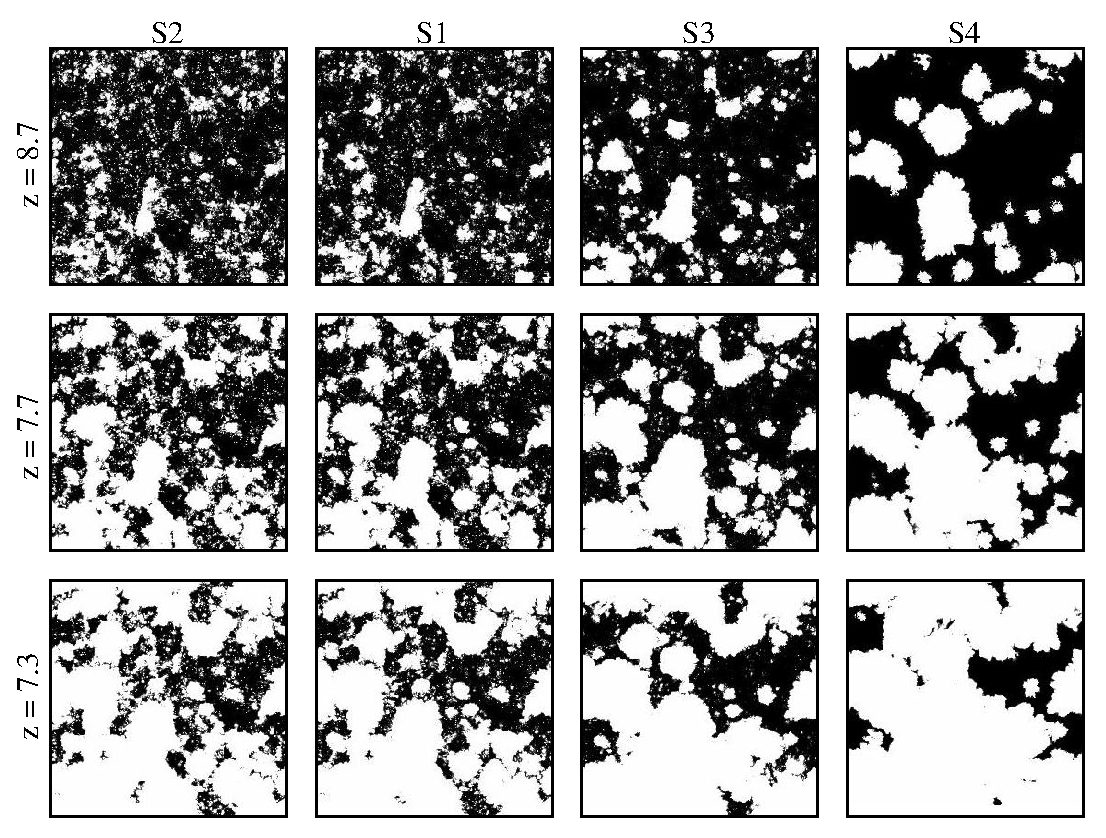
\includegraphics[width=7in]{chap0_intro/mcquinn_ionized_region_sims.eps}
	\caption[aoeuaoeu]{aeuoaoeu. Reproduced from \citet{McQuinn06}}
	\label{fig:mcquinneorsims}
\end{figure}



\subsection{Evolution of the global 21\,cm signal}

In this section we seek a sense the magnitude of the mean 21\,cm signal over cosmic time. Indeed as we saw, the brightness temperature of the 21cm signal is determined by the spin temperature, which is affected by three processes: collisional coupling with atoms and free electrons which couple the gas kinetic temperature to the spin temperature, radiative coupling to the CMB, and Ly$\alpha$-induced spin-flips via an excited state. 

As the universe evolves, the relative importance of each of these processes changes, and the spin temperature evolves accordingly. Fig. \ref{fig:pritchardloebtemperatures} shows the gas, spin, and CMB temperatures (top), the ionized fraction (center), and the differential 21\,cm brightness temperature (i.e., the 21\,cm spin temperature relative to the CMB (bottom) as a function of redshift. Three different reionization models, giving different spin and differential brightness temperature histories are presented. At $1100>z>200$ (A), the universe is dense enough so that collisional coupling between atoms and residual free electrons holds $T_\text{gas}\approx T_\gamma=T_s$, so the relative 21\,cm brightness temperature is close to zero. Then over $200>z>50$ the gas cools adiabatically, implying\footnote{Adiabatic cooling implies $PV^\gamma=$const, where $\gamma=c_p/c_v=1+1/c_v$. For a monotonic ideal gas, the specific heat at constant volume is given by $c_v=3/2$. Note also that $TV^{\gamma-1}=$const, which gives $T\sim (1+z)^2$} $T\sim (1+z)^2$. The spin temperature thus cools a factor of $1/(1+z)$ faster than the CMB, so the differential brightness temperature becomes negative (B). Note that the gas is cooling below the CMB temperature, but the gas temperature is still coupled to the spin temperature. At these high redshifts, structure is still largely linear, so that the brightness temperature traces the matter density field without corrupting \textit{gastrophysics}\footnote{Gastrophysics is a neologism refering to the astrophysics (i.e., non-cosmological) effects on the 21\,cm signal due especially to non-linear galaxy formation and feedback effects which are challenging to model.} 

\begin{figure}
	\centering
	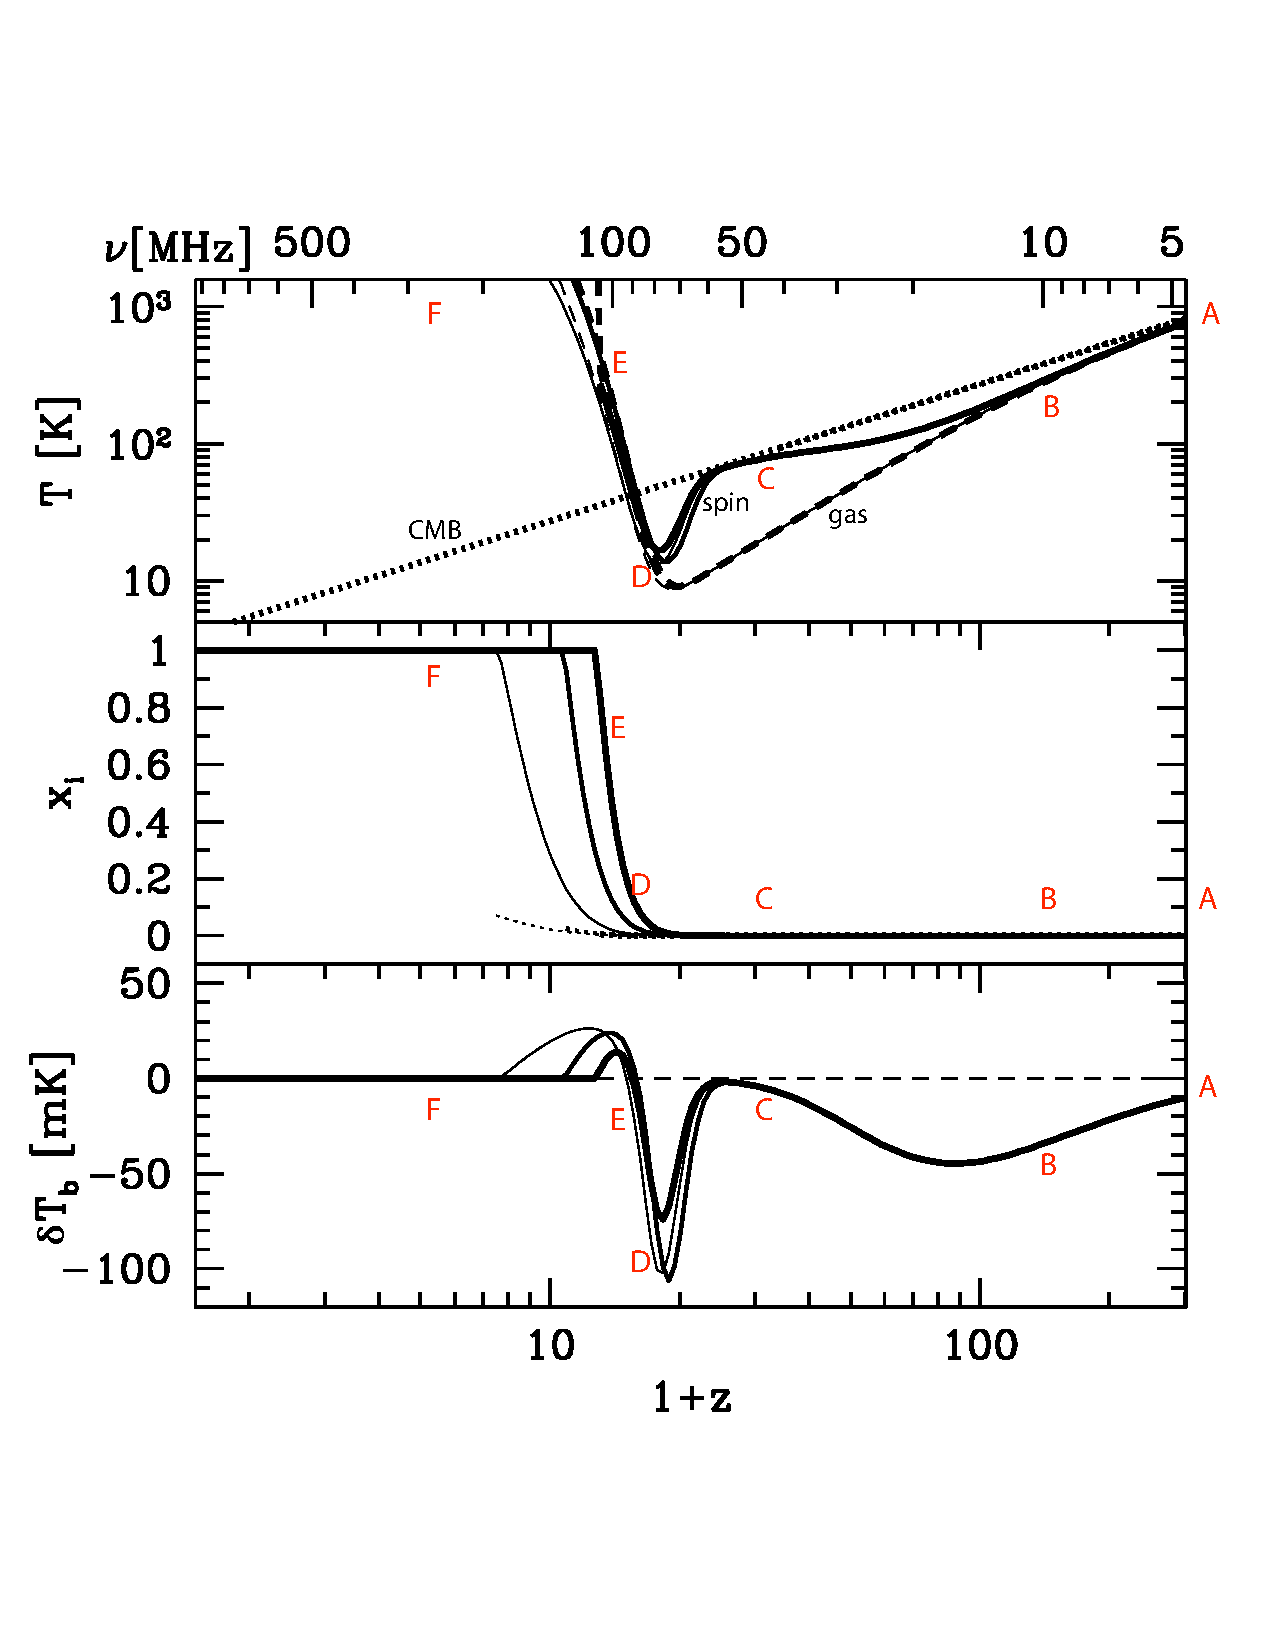
\includegraphics[width=7in]{chap0_intro/pritchard_and_loeb_temperatures_annotated.pdf}
	\caption[aoeuaoeu]{aeuoaoeu. Reproduced from \citet{PritchardLoebReview}}
	\label{fig:pritchardloebtemperatures}
\end{figure}

From here on, the exact sequence of events becomes quite uncertain. It is thought that as the universe continues to expand, the gas becomes too dilute for collisions to couple the gas and spin temperatures, and the spin temperature falls back into equilibrium with the CMB, reducing the differential brightness temperature towards zero (C). When the first sources form and begin to emit ionizing radiation, the Ly$\alpha$-induced spin flops mentioned above couple the spin temperature back to the gas temperature, which at this point is much colder than the CMB (D). In quick succession, heating of the IGM from this radiation becomes significant, raising the 21\,cm signal over the CMB temperature (E), until the bulk of the universe becomes ionized and there are no further large neutral regions to emit 21\,cm radiation (F).

\section{Measuring the 21\,cm signal with radio interferometers}

\subsection{The basics of radio interferometry}

A radio interferometer is an array of separate antennas whose outputs are correlated with each other, and combined to form an image. It is ofter cheaper and easier to use such a ``synthetic aperture'' to resolution and collecting area than to simply build ever bigger single dish antennas, especially given advances in computing over the past decades permitting real time correlation of hundreds of antennas. In this section I will review how we get from the individual antenna outputs to a sky image for a simple 1D array viewing a 1D sky.

\begin{figure}[h]
    \centering
    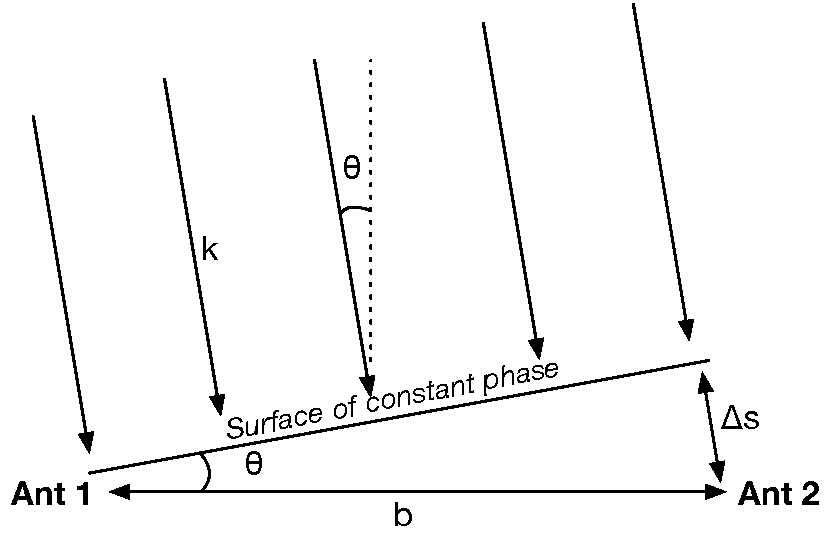
\includegraphics[width=0.95\textwidth]{chap0_intro/radio_interferometer_diagram.pdf}
    \caption[Diagram of a two element radio interferometer]{A single baseline (i.e., pair of antennas) displaced by $b$ on the ground receive radiation from a distant source at an angle $\theta$ from zenith. The source is distant enough that its surfaces of constant phase are planes which are orthogonal to $\vec{k}$, the wavevector of the radiation. The radiation arriving at Antenna 1 accumulates extra phase due to the path length difference $\Delta s$ compared to that arriving at Antenna 2.}
    \label{fig:radiointerferometerdiagram}
\end{figure}

Consider first a pair of antennas (termed a \textit{baseline}) on the ground separated by distance $b$. Radiation arrives from a distant source at an angle $\theta$ from zenith. Observe (Fig. \ref{fig:radiointerferometerdiagram}) that after the surface of constant phase reaches the first antenna, must it propagate an extra distance $\Delta s$ before reaching Antenna 2, equaling an extra phase of $\vec{k}\cdot \vec{b}=2\pi\Delta s/\lambda=2\pi\sin b/\lambda$. Then the time averaged cross correlation between the voltages measured at antenna 1 and 2, known as the visibility $V_{12}$, is
\begin{equation}
	V_{12}\equiv\langle V_1(t)V_2^*(t)\rangle=\langle(V_0^* e^{i\omega t})(V_0e^{-i(\omega t-2\pi\sin u)})\rangle \approx e^{2\pi i b\theta/\lambda}
\end{equation}
where we have used the small angle approximation, and we have switched to measuring the baseline length in units of wavelengths $u\equiv b/\lambda$. We can see that $u$ and $\theta$ are fourier dual variables. If we can measure the visibility at many different baseline lengths, then we can grid them in $u$ space and take the fourier transform to get their representation in the $\theta$ space, which is simply the sky image.

Real world interferometers have non-uniform and incomplete sampling in $u$ space, encoded by a sampling function $S(u)$. We may view this function as a sum of delta functions located at all the sampled $u$ values: $S(u)=\sum_{i,j}\delta(u_i-u_j)$, where $i,j$ index the antennas. Multiplying the true visibility function $V(u)$ by this sampling function, then fourier transforming, is equivalent (by the convolution theorem) to convolving the true sky image by the fourier transform of the sampling function, known as the synthesized beam. This is known as the \textit{dirty image}. Unlike in optical astronomy where the point spread function is close to a gaussian or an Airy function, the synthesized beam is generally non-compact with significant sidelobes due to sparse baseline sampling.  

The strategy is typically to distribute the antennas pseudo randomly to achieve as many different baselines as possible, calculate the dirty image, then use an iterative procedure known as CLEAN \citep{hogbomclean} to incrementally deconvolve the synthesized beam from the true sky image under the assumption that the true sky is predominantly a collection of isolated point sources. The statistics of the resulting \textit{clean image} are difficult to quantify as CLEAN is a non-linear algorithm, but in practice it is found to work quite well and is indispensable to characterizing the compact radio sources between us and the EOR signal (i.e., foregrounds).

\subsection{From image cubes to power spectra}

First generation experiments lack the sensitivity to directly image 21\,cm emission from the EOR, aiming instead to statistical detections of the signal through different methods of combining many pixels, each with SNR<1, into a significant detection. The most prominent of these methods is estimation of the power spectrum.

To understand how cosmological power spectrum measurements are made, let us first consider the space the interferometer measurements live in. Interferometer measurements consist of cross correlations, or visibilities, at different frequencies. We have shown in the previous section that each visibility is a measurement of a different sky fourier mode $(u,v)$, which are dual coordinates to $(\theta_x,\theta_y)$. However, each frequency corresponds to a different cosmological redshift, and thus, distance from us. Interferometric visibilities thus live in an awkward mixed fourier space: To study foregrounds, we must fourier transform along $u$ and $v$ to reach 3D image space, but to make power spectrum measurements, we must transform along $f$ to reach 3D fourier space. This is illustrated in Fig. \ref{fig:ifospace}, where we denote the fourier dual to $f$ as $\eta$, termed \textit{delay}.

\begin{figure}[h]
    \centering
    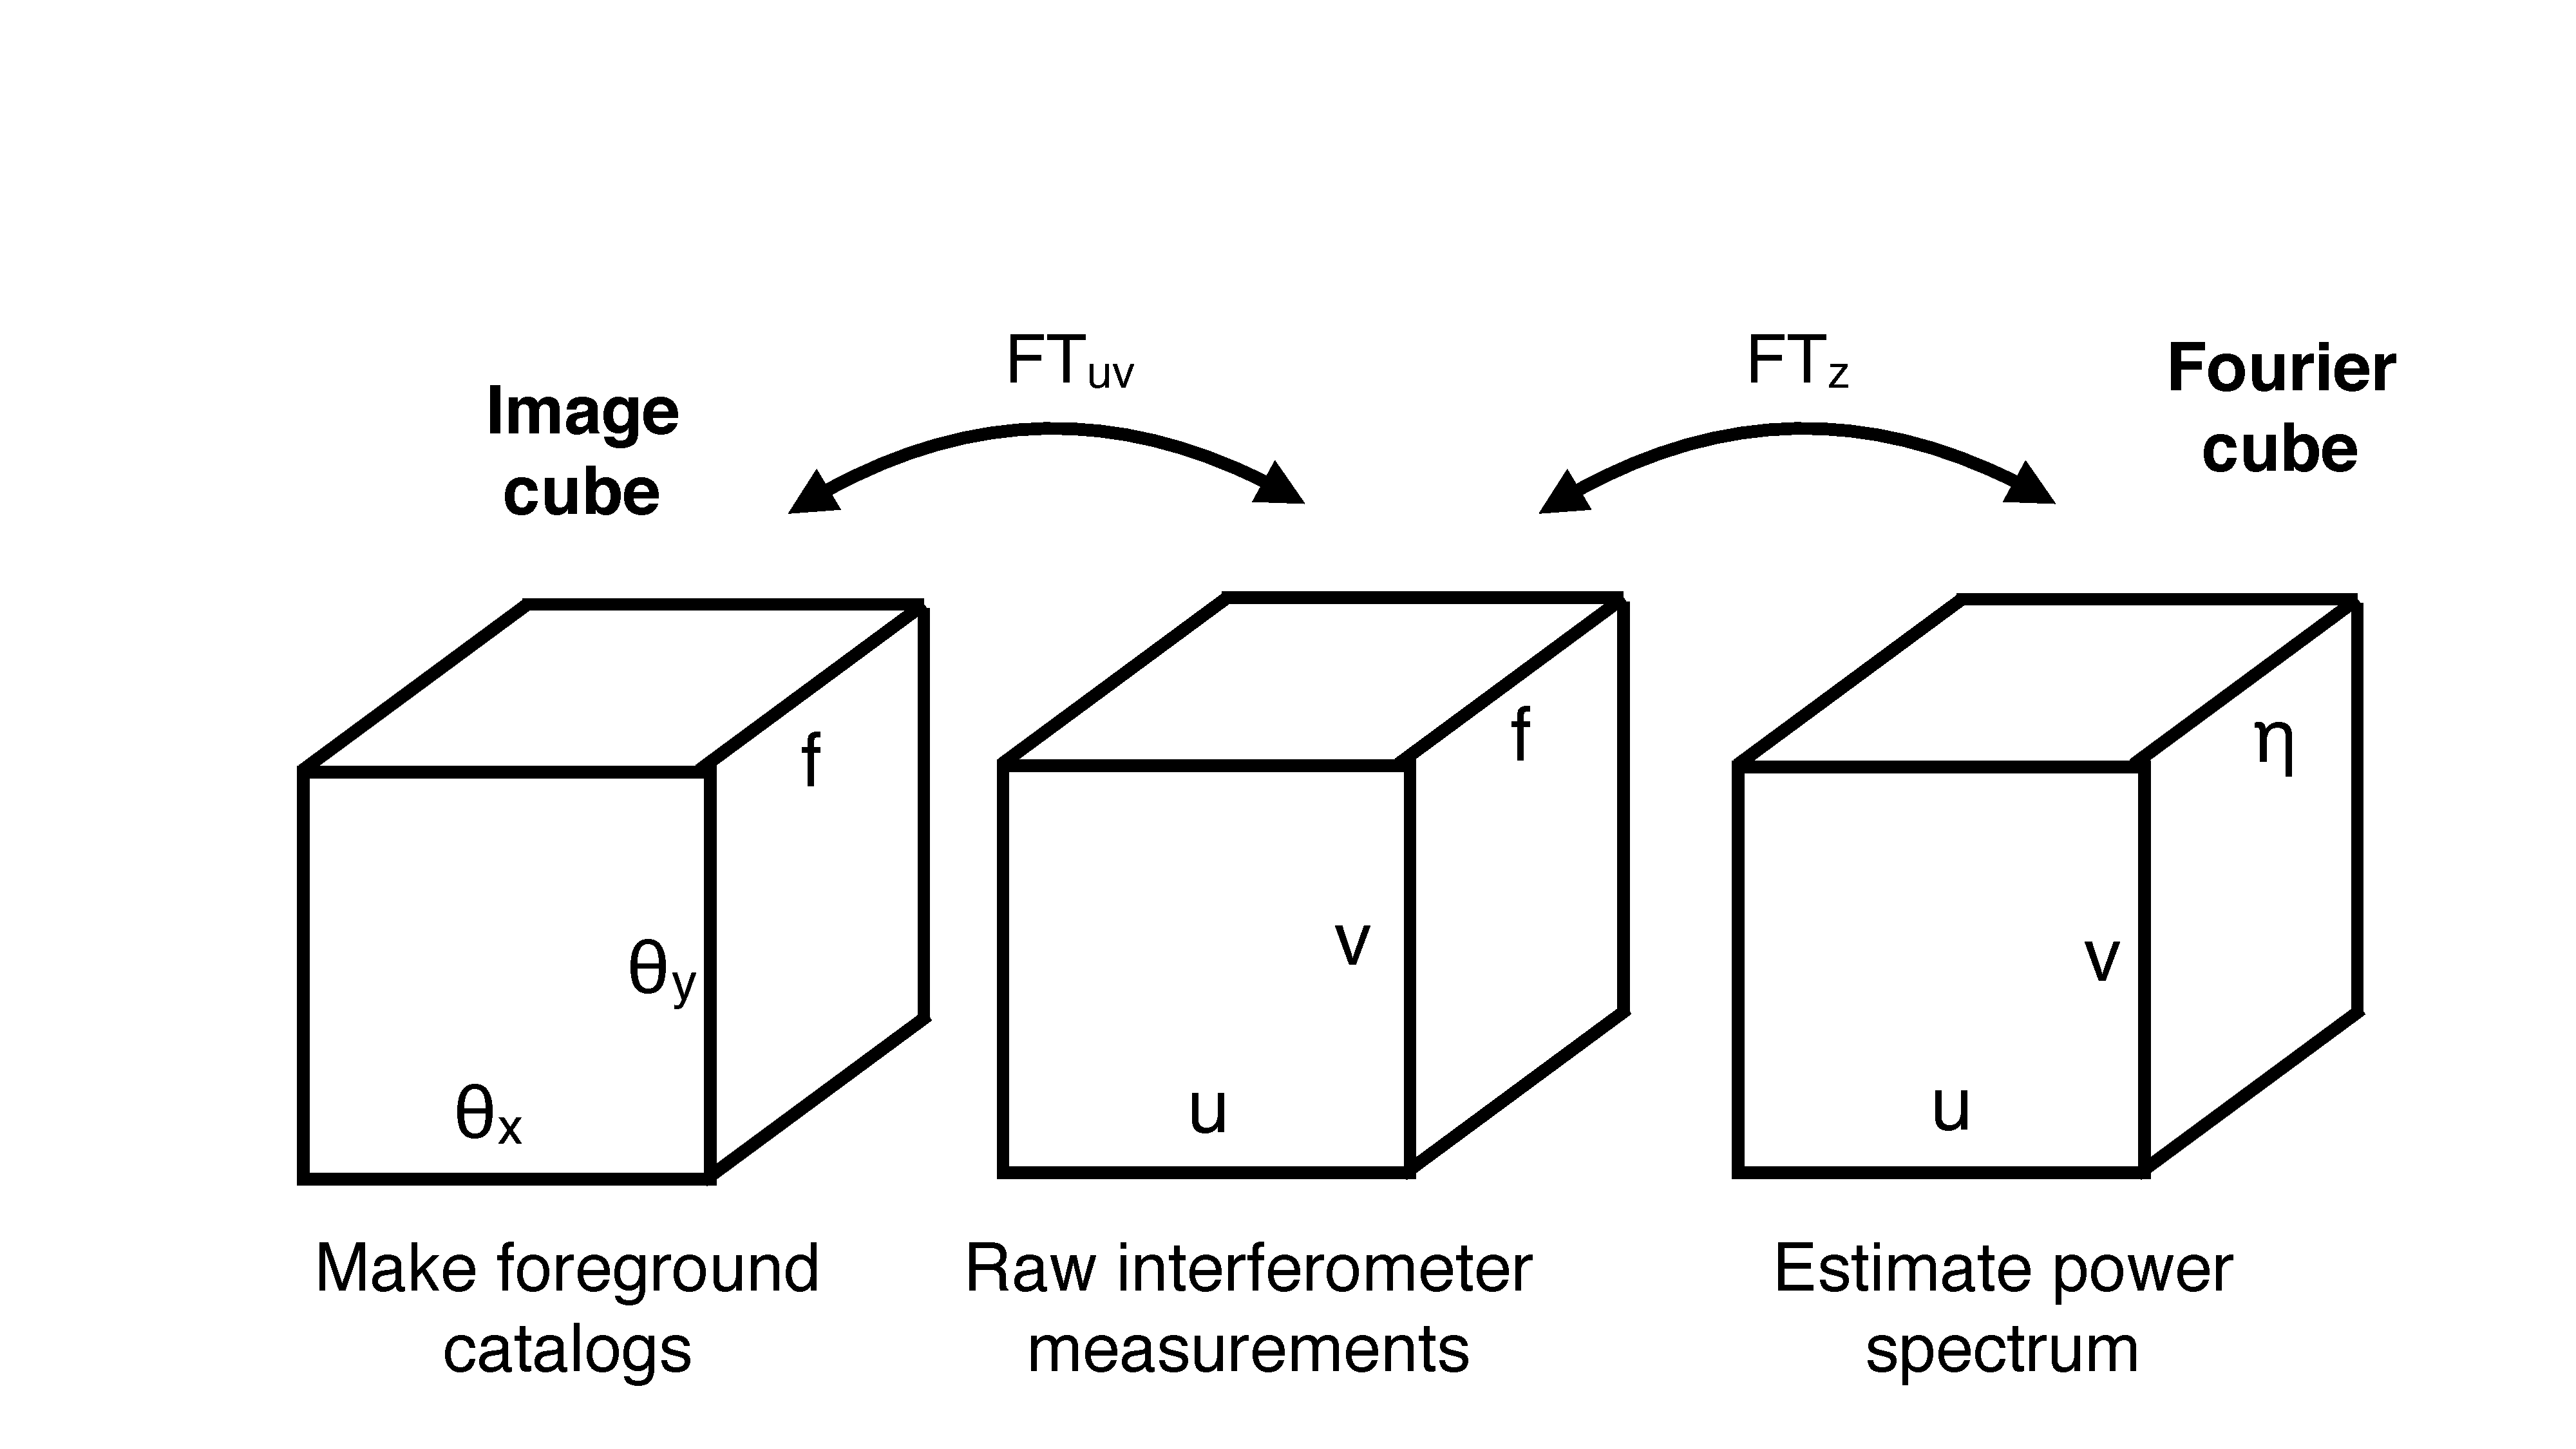
\includegraphics[width=1\textwidth]{chap0_intro/ifo_space.pdf}
    \caption[Representation of the relation between image space, fourier space, and interferometer space]{aoeuaoeu}
    \label{fig:ifospace}
\end{figure}

We seek to estimate the spatial power spectrum of 21\,cm emission in comoving units, that is, as a function of wave number $k$ with units of inverse comoving distance. We must first transform $u$ and $v$ to $k_x$ and $k_y$. For brevity, consider only the $x$ dimension. $u$ is defined by the fourier factor $e^{2\pi i u\theta}$, which we must match with $k_x$, defined by $e^{ik_x x}$, where $x$ is the comoving distance transverse to the line of sight. Setting their exponents equal and using $x=D\theta$, where $D$ is the comoving distance to the redshift of interest, we find.

\begin{eqnarray}
	k_x=\frac{2\pi u}{D} \\ 
	k_y=\frac{2\pi v}{D} \\ 
\end{eqnarray}

To relate $k_z$ to $\eta$, we must first match the exponents in $e^{i k_z x_\parallel}$ and $e^{i\omega \eta}$, where $x_\parallel$ is the comoving distance along the line of sight\footnote{Unfortunately we can't refer to this as $z$ because it's taken by the cosmological redshift.} and $\omega=2\pi f$ gives the observation frequency. Matching these, and using that $d x_\parallel/df=cf_0/H(z)f^2$, we find

\begin{equation}
	k_z=\frac{2\pi\eta f_0 H(z)}{c(1+z)^2}
\end{equation}

\begin{figure}[h]
    \centering
    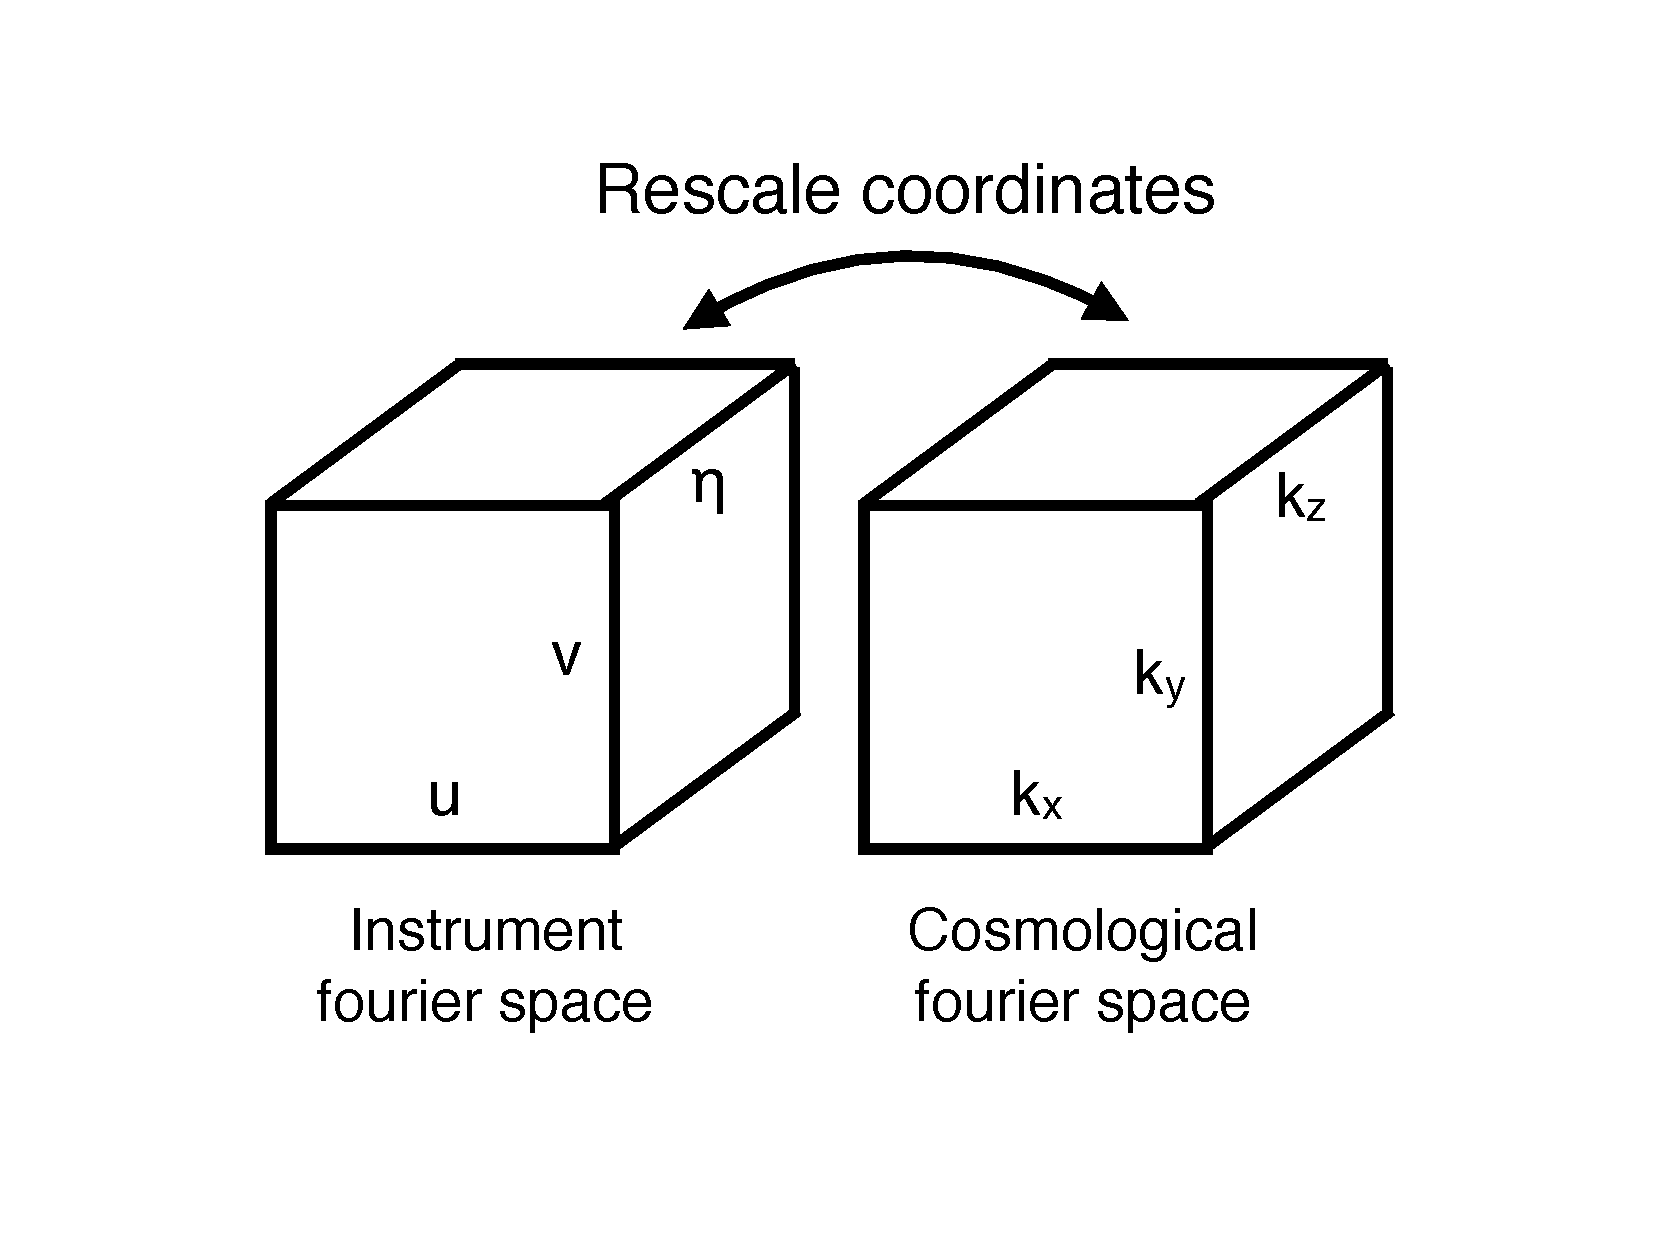
\includegraphics[width=0.9\textwidth]{chap0_intro/ifo_space_cosmo.pdf}
    \caption[Representation of the relation between image space, fourier space, and interferometer space]{aoeuaoeu}
    \label{fig:ifospacecosmo}
\end{figure}

A last note is that to characterize foregrounds, we often combine $k_x$ and $k_y$ together to plot the \textit{cylindrically} binned power spectrum as a function of $k_\perp\equiv(k_x^2+k_y^2)^{1/2}$ and $k_\parallel\equiv k_z$.

%optimal quadratic power spectrum estimators, essentially, generalized FT with arbitrary weighting



\subsection{Sensitivity challenges}
\label{sec:sensitivity}

The two major challenges to observing redshifted 21\,cm emission from the dark ages and EOR are sensitivity and foregrounds. Interferometers at low frequencies are sky noise dominated, meaning that the diffuse galactic synchrotron dominates the received antenna power, and thus, the visibility noise. However it is so diffuse, and thus, so compact in $uv$ space, that its contribution to the visibility means is negligible. See Appendix A for a full discussion of sky noise. Our concern here is that in the coolest parts of the sky, at high galactic latitudes, galactic synchrotron has brightness temperatures of $\sim200$\,K \citep{Tsysmemo}. The cosmological global signal is at the tens of mK level, and simulations suggest that individual fourier modes are far smaller, at the few mK level. 

Let us get a sense for the sensitivity challenge with a rough calculation. I show in Appendix A that the noise $\sigma_V$ on visibility $V_{ij}$ is given by $V_{ii}/\sqrt{Bt}$ where $V_{ii}$ is the autocorrelation, $B$ is the bandwidth, and $t$ is the observation time. Measuring the sky in brightness temperature units, the autocorrelation is given by $V_{ii}=\int T(\hat\theta)d\Omega\sim T_\text{sky}\Omega$, where $\Omega=\lambda^2/A$ is the solid angle of the beam main lobe. Comparing this brightness temperature noise with the expected few mK cosmological visibilities, gives roughly 100 hours for a 5$\sigma$ detection. Note that this is not the total length of time observing. As the earth rotates, baselines are projected and rotated to different parts of the $uv$ plane. Over several hours of observing, many baselines enter and exit the $uv$ cell in question, and in general many more than 100 hours of observing is needed to achieve 100 hours in each cell. 

However, as alluded to above, we don't need 5$\sigma$ detections in every $uv$ cell to make a detection of the power spectrum of 21\,cm emission. Consider a simple case where we neglect the frequency dimension. Let raw visibilities have noise $\sigma_V$, and each $uv$ cell is the average of $N_\text{vis.per.cell}$ of them. Then the power spectrum is is estimated by averaging the power over the $N_\text{cells}$ cells with similar $\sqrt{u^2+v^2}$ magnitude. The noise on the mean visibility $\bar{V}$ in each cell is $\sigma_V/\sqrt{N_\text{vis.per.cell}}$, and the noise $\sigma_{\bar V^2}$ is $\sqrt{\langle\bar V^4\rangle-\langle\bar V^2\rangle^2}\sim\sigma_V/\sqrt{N_\text{vis.per.cell}}$, which is reduced by $1/\sqrt{N\text{cells}}$ when spherically binning. So we find 

\begin{equation}
	\sigma_P\propto\frac{\sigma_V^2}{N_\text{vis.per.cell}\sqrt{N_\text{cells}}}
\end{equation}

Thus we see that there are two kinds of averaging which reduce the level of thermal noise in the power spectrum: \textit{coherent} averaging (by a factor of $1/N_\text{vis.per.cell}$) within individual $\vec{k}$ modes, and \textit{incoherent} averaging (by a factor of $1/\sqrt{N_\text{cells}}$) of power over different $\vec{k}$ modes falling into the same spherical $k$ bin. In the first case, we average different measurements of the same true value but with different noise, whereas in the second case, we average different realizations of the true spherical bandpower $k$. Were there no thermal noise on our measurements, the first average would do nothing, but the second would help to reduce sample variance noise. 

So we see that sensitivity of a real interferometer is set by the amount of coherent and incoherent binning of thermal noise, due to the 200\,K diffuse galactic synchrotron emission.  \citet{beardsley13} predict a $7\sigma$ detection of the power spectrum with the Murchison Widefield Array after 450\,hours, and \citet{PoberNextGen} predict a 3--7$\sigma$ detection after 1080\,hours, depending on foreground properties. In contrast to the MWA, whose antennas are distributed pseudo randomly to maximize the number of $uv$ modes sampled, PAPER's antennas are placed on a grid. Thus very few $uv$ modes are sampled, which makes imaging extremely challenging, but from a power spectrum point of view, they have optimized for coherent averaging at the expense of incoherent averaging. \citet{PoberNextGen} thus predict comparable sensitivities to the MWA despite their substantially smaller antennas. HERA builds on both sets of lessons learned, employing ultimately 350 14\,m dishes on a grid, and should yield tens of $\sigma$ detection \citet{neben16b,ewallwice16,nithya16,PoberNextGen}. 

\subsection{Foreground challenges}

While the diffuse synchrotron emission in our galaxy generates the noise on our measurements, compact extragalactic radio sources between us and the EOR generate a bias. We term these these sources \text{foregrounds}, though the rest of the astronomy community terms them \textit{science}. Over the 100-200\,MHz band corresponding to redshifted 21\,cm emission from the EOR, foreground emission is sourced by radio synchrotron generated by relativistic electrons gyrating around galactic magnetic field lines. I derive in Appendix \ref{chap:synchrotron} that synchrotron emission has a power law spectrum with $I\sim\nu^{-0.75}$.

The smooth spectral structure of foregrounds is key to distinguishing them from the blotchy reionizing universe (Fig. \ref{fig:mcquinneorsims}). A line of sight through the EOR passes through some neutral regions and some ionized regions, making the overall 21\,cm emission from the neutral regions, all at slightly different redshifts, appear spectrally very unsmooth. Early work proposed removing smooth structure  from every line of sight through the cube separately, subtracting splines, low order polynomials, or eigenforegrounds \citep{Judd08, paper1, paper2,xiaomin,LOFAR2,Harker,Jelic08,MoralesBowmanHewittFGsub}. However, simulations \citep{Dattapowerspec}, early theory \citep{VedanthamWedge,MoralesPSShapes,CathWedge,nithya13}, and early data analyses have shown that this is not the whole story. The frequency-dependent $uv$ sampling of interferometer baselines causes spectrally smooth foreground power to leak into higher $k_\parallel$ modes. Said differently, as a function of frequency, each baseline samples a different fourier mode of the sky, and that effect cannot be perfectly removed by simply gridding the baseline to a different $uv$ cell at different frequencies. Longer baselines move through $uv$ space faster with frequency, and this linear dependence manifests after gridding many baselines to $k_\perp,k_\parallel$ space as wedge-shaped region containing the preponderance of foreground power. 

Work to understand this leakage is ongoing. \citet{AdrianWedge1,AdrianWedge2} show that it introduces not only a bias to the power spectrum but error correlations as well. It also manifests differently \citep{pober13} in the approximate power spectra computed using the per-baseline technique of \citet{parsonsandbacker,parsons12b} than using the image-based power spectra of \citep{beardsley16,dillonneben,X13}. 

Knowing this, two basic approaches to foreground removed have been discussed in the literature: foreground avoidance and foreground subtraction. The former consists of simply excluding modes in the wedge from power spectrum estimation, albeit at a non-negligible sensitivity hit, while the latter requires subtraction of 99.99\% of foreground intensity. Both are challenging, and neither has yet resulted in an EOR detection, but new experiments such as the under-construction HERA \citep{neben16,ewallwice16,nithya16,deboer16} and the next generation SKA \citep{ska,ska1,ska2,ska3} should achieve highly significant detections in even the most pessimistic foreground cases. 

\subsection{Large N--small D arrays and their challenges}

In this section I will introduce the class of experiments being conducted to observe spatial fluctuations in 21\,cm emission from the EOR, and outline the experimental challenges they pose. As discussed in Sec. \ref{sec:sensitivity}, detection of 21\,cm from the EOR demands hundreds of hour integrations on arrays with hundreds of antennas. Even so, arrays such as MWA, PAPER, LOFAR, and now HERA are targeting only a statistical detection of the emission, that is, detection of a smooth power spectrum rather than high SNR images of ionizing bubbles. The latter demands even more sensitivity, and must await the Square Kilometer Array, an array planning literally nearly a square kilometer of antenna collecting area on the ground. 

With these enormous demands on collecting area, cost of a handful of enormous dishes would be prohibitive, especially as it would need to steer around the sky to avoid foregrounds and the galactic plane. Typical radio interferometers over the past decades have consisted of a few or a few dozen steerable dishes such as the Very Large Array, the Giant Meterwave Radio Telescope, the Westerbork Synthesis Radio Telescope, and now the Atacama Large Millimeter Array. 

The 21\,cm arrays listed above instead represent a new generation of low frequency radio interferometry made possible by advances in large scale digital signal processing, computing, and storage. Indeed PAPER was so named after Don Backer's famous aphorism that what was required to detect the EOR was ``paperclips and supercomputers.'' At meter-wavelengths, antenna fabrication precision is largely irrelevant, and pointing is done far more cheaply with beamforming (ie, by placing smaller antennas into phased arrays) than with steerable dishes. 

Effectively eschewing hardware investment for software investment is not without its challenges, though, in fact many traditional techniques of radio astronomy are proving insufficient and the community is grappling with how to improve them. Work on better antenna measurement, gain and phase calibration, radio frequency interference flagging, source cataloging, and quality control is ongoing in order to make cosmological 21\,cm observations a reality, and this thesis is part of that larger effort. Over the remainder of this section, I will outline the specific challenges that large N--small D arrays are posing experimentally, and what is being done to address them.

\begin{itemize}
	\item \textbf{Antenna measurement} 
	\item \textbf{Gain and phase calibration} 
	\item \textbf{Quality control} 
	\item \textbf{Source cataloging} 
\end{itemize}



big data / quality control (cite beardsley)
\citep{beardsley16}

primary beam measurements, wide field problem, no clean fields

gain calibration: sky models are imperfect at low frequencies, cite Aaron EW's recent calibration paper, an Braun, cite danny's precision+accuracy paper
\citep{jacobs2013,braun2013,ewallwice16b}

a slightly bigger antenna element has an advantage (HERA)
\citep{deboer16}

%\section{Roadmap of this thesis}


%\section{Completing the picture with cross correlations}
%
%\subsection{examples of successful cross correlation results}
%Tzu-Ching's result \citep{Chang2010,Masui2013}
%
%\subsection{what could be learned from IR cross correlation}
%more about the sources: pop2 vs pop3
%topology of reionization, anticorrelation scale shows bubble size increasing over time
%
%\citep{Heneka2016}
%\citep{Fernandez2014,Silva2012,Mao2014,Lidz2008,Gong2014,Fernandez2013}
%


\chapter{Measuring High Dynamic Range MWA Beampatterns using 137 MHz ORBCOMM Satellites}
\label{chap:beampaper}

The content of this chapter was originally published as Neben, A.R. et al., \textit{Measuring phased-array antenna beampatterns with high dynamic range for the Murchison Widefield Array using 137 MHz ORBCOMM satellites}, Radio Science, 50:614–629, July 2015. doi: 10.1002/ 2015RS005678. Rich Bradley developed the digital signal processing hardware which samples, accumulates, fourier transforms, and averages the antenna signals, and wrote the original code to cross match observed satellite passes with predicted satellite positions. Jackie Hewitt and I assembled the MWA prototype tile at Green Bank, and I wrote code to combine measured voltages and calibration measurements into beampatterns for the MWA antenna. I also implemented automated quality control cuts and averaged beam measurements in sky pixels to drastically improve the measurement accuracy, then did a thorough error analysis of the measurement system and the systematics in our prototype MWA antenna tile. I wrote the paper about our results.  \\

Detection of the fluctuations in 21 cm line emission from neutral hydrogen during the Epoch of Reionization in thousand hour integrations poses stringent requirements on calibration and image quality, both of which necessitate accurate primary beam models. The Murchison Widefield Array (MWA) uses phased array antenna elements which maximize collecting area at the cost of complexity. To quantify their performance, we have developed a novel beam measurement system using the 137 MHz ORBCOMM satellite constellation and a reference dipole antenna. Using power ratio measurements, we measure the {\it in situ} beampattern of the MWA antenna tile relative to that of the reference antenna, canceling the variation of satellite flux or polarization with time. We employ angular averaging to mitigate multipath effects (ground scattering), and assess environmental systematics with a null experiment in which the MWA tile is replaced with a second reference dipole. We achieve beam measurements over 30 dB dynamic range in beam sensitivity over a large field of view (65\% of the visible sky), far wider and deeper than drift scans through astronomical sources allow. We verify an analytic model of the MWA tile at this frequency within a few percent statistical scatter within the full width at half maximum. Towards the edges of the main lobe and in the sidelobes, we measure tens of percent systematic deviations. We compare these errors with those expected from known beamforming errors. 

\section{Introduction}

% motivation for the measurement
The prospects of studying the formation of the first structures in the universe at $z\sim6$ and earlier with 21 cm hydrogen emission have driven investment in a new generation of low frequency radio astronomy instruments (see \citet{FurlanettoReview, miguelreview, PritchardLoebReview, aviBook, zaroubi} for reviews). The extreme surface brightness sensitivity required to detect the 21 cm signal in the presence of galactic, extragalactic, and thermal noise backgrounds has pushed this generation of experiments into an untested regime. Uncertain primary beams and source catalogs, in addition to wide fields of view, complicate analysis and demand new methods of calibration, imaging, and primary beam characterization. 

A number of experiments now operating, such as the Murchison Widefield Array (MWA) \citep{lonsdale09,tingay13,mwascience}, the Donald C. Backer Precision Array for Probing the Epoch of Reionization (PAPER) \citep{parsons14}, and the LOw Frequency Array (LOFAR) \citep{lofar}, as well as demonstrator instruments like the MIT Epoch of Reionization Array (MITEoR) \citep{zheng14}, next-generation experiments like the Hydrogen Epoch of Reionization Array (HERA; \citet{PoberNextGen}; http://reionization.org), and future instruments like the Square Kilometer Array \citep{ska} have opted for large arrays (hundreds of elements) of non-pointing or only coarsely-pointing antennas, attempting to balance collecting area and cost considerations. For all these experiments, \textit{in situ} high-fidelity primary beam characterization remains a major challenge given the high dynamic range \citep[e.g.][]{AaronSensitivity, beardsley13, nithya13, PoberNextGen} thought necessary to reveal the cosmological 21 cm signal. 

Recovering the 21 cm signal in the presence of strong foregrounds is made easier by taking advantage of an effective containment of smooth spectrum foregrounds in a Fourier space region knows as the ``wedge'', despite the frequency-dependent response of the interferometer \citep{Dattapowerspec,X13, pober13,MoralesPSShapes, VedanthamWedge, nithya13, CathWedge, AdrianWedge1, AdrianWedge2}. However, frequency dependent systematics due to insufficiently accurate primary beam modeling for calibration or primary beam correction may cause foreground leakage out of this compact region. This would shrink the region within which a cosmological power spectrum measurement can be made and thus lower the significance of a detection \citep{PoberNextGen}. In fact, \citet{nithya15,nithya15b} show that most pernicious for such measurements is sky emission from large zenith angles, even near the horizon, just where beampatterns are most difficult to model. Ultimately, the full polarization response may be needed to best model and subtract polarized sources that can leak a sinusoidal frequency signal into Stokes I due to their Faraday rotation \citep{jelic2010,moore13}. Recent measurements \citep{bernardi13, moore13,moore15,asad15} indicate that most of the high rotation measure sources are, however, largely depolarized at low frequency.%, making accurate polarization beam measurements less demanding than previously anticipated.

Though brought to the forefront again by 21 cm science, primary beam measurements have a long history in radio astronomy and electrical engineering. Radio astronomers typically rely upon celestial radio sources with known flux densities to measure beampatterns as the sources trace out cuts through the beam \citep[e.g.,][]{nithyaVLA}. If the beam is narrow enough for the sky to appear as a single point source, knowledge of its flux density is not needed to measure relative beam sensitivity along its track \citep[e.g.][]{colegate14}, though combining tracks from different sources, or using fields with multiple sources requires accurate knowledge of their relative fluxes. Indeed, the wide fields of view of dipole elements and uncertainties in low frequency source catalogs make this analysis difficult and entangled with calibration \citep{jacobs2013}. Further, the lack of axial symmetry in non-dish antennas around the antenna pointing direction makes a complete beampattern impossible to measure from just a handful of cuts. Relying only on the weaker assumption of $180^\circ$ rotation symmetry, \citet{pober12} present an interferometric beam measurement technique making use of celestial sources with unknown flux densities, assuming the data are already calibrated.  

% state of the art in sat beam measurements
In this paper we pursue an alternate approach based on probe signals from satellites. Satellite-based antenna beampattern measurements have many clear advantages over astronomical sources. Satellites are substantially brighter, and thus dominate in otherwise crowded fields and probe deep into beam sidelobes. They also make many cuts through the beam over the course of many orbits, due to precession. \citet{brueckmann63} exploited these advantages in early satellite measurements of antenna beampatterns. Lingering issues such as varying antenna pointing and plane of polarization (due to Faraday Rotation or simple projection effects) and time-varying satellite transmitter power may be solved through use of a simple, well-understood reference antenna and power ratio measurements, which measure the relative beampattern of the Antenna-Under-Test (AUT) \citep[eg.][]{fukao85, law97, hurtado2001, vlbamemo}. This approach has been used to great effect in holographic antenna measurements \citep{rochblatt92, harp2011, lasenby85, godwin86, deguchi93}, with at most a handful of satellites.

% general overview of our approach and paper contents
As a first step towards antenna beam measurements exploiting all these advantages for 21 cm cosmology and for the MWA, we develop a prototype of a novel beam measurement system using probe signals from the 137 MHz ORBCOMM satellite constellation and a reference dipole antenna. The precession of these low Earth orbit satellites and their sheer number ($\sim30$) yield $65\%$ coverage of the visible sky (limited by satellite coverage at our Green Bank site) at $2^\circ$ resolution in a single day. Early tests and demonstrations of our initial concept were presented by \citet{ries07, BradleyAndRies2008,CzekalaAndBradley2010,CzekalaAndBradley2010_2,aasposter}, and recently,  \citet{zheng14} have demonstrated a simple implementation of this concept in a working interferometer. We use an ORBCOMM interface box to determine satellite transmission frequencies on the fly, allowing us to take advantage of even more of the ORBCOMM signals in an automated manner.

In this work, we present the full working power pattern mapping system, as well as an error analysis of environmental systematics such as multipath (ground scattering). We expect the lessons learned about these systematics to inform future beam measurements and array calibration methods employing probe signals carried by remote-controlled drones or satellites. 

We use our working beam measurement system to make the first precision measurements of an MWA tile in a deployment-style environment over a large fraction of sky. Each MWA tile is a $4\times4$ grid of bowtie dipoles, optimized to have a broad frequency response over 80--300 MHz, whose signals are combined in a delay-line beamformer. This design results in a large collecting area per tile and a beam narrow enough to steer away from the bright galactic disk and terrestrial RFI, but adds model complexity and uncertainty near the edges of the main beam and in the sidelobes (grating lobes). Indeed the MWA tile design poses simulation challenges due both to potential dipole cross coupling effects as well as the large number of degrees of freedom which must by simulated (hundreds of frequencies, dozens of pointings, and fine angular resolution). Note, though, that current processing of MWA data utilizes simulated beampatterns, and experiments such as that presented in this work aim more to assess their validity than to replace them with measurements.

Early beampattern measurements of deployed prototype MWA tiles using source drift scans \citep{bowman07} and anechoic chambers \citep{williamsthesis2012} revealed rough agreement with models. Yet $\sim1$ dB deviations were observed throughout the main lobe and $3-5$ dB deviations in sidelobes, highlighting the need both for better modeling and better control of measurement systematics. Later, \citet{sutinjo15} found that upwards of 200 MHz, interactions between antennas necessitate more complex modeling than simple multiplication of a Hertzian dipole beampattern by the array factor. We are interested here in characterizing the deviations from ideality at lower frequencies where the simple model is more likely to hold. At some level, the beams are expected to be corrupted by beamforming amplitude and phase errors, finite ground screen effects, as well as any dipole-dipole interactions. We compare our measurements with an empirical budget of beamforming errors due to dipole phase and gain mismatching which we present in a separate paper \citep{neben16}.

In Section \ref{sec:measurementsystem} we discuss our beam measurement system including the ORBCOMM satellites, our reference antenna, and our data acquisition system. We discuss our data analysis pipeline in Section \ref{sec:analysis} and also present results of a null experiment in which a second reference antenna is used as the Antenna-Under-Test. We present beam measurements of our MWA tile and compare with models in Section \ref{sec:mwatile}, and conclude with discussion and conclusions in Section \ref{sec:discussion}.

\section{Measurement System}
\label{sec:measurementsystem}

\subsection{Overview}

Figure \ref{fig:systemoverviewdiagram} shows a schematic diagram of our antenna setup and measurement chain. A reference antenna (see Section \ref{sec:refant}) and an Antenna-Under-Test (AUT) both pick up transmitted signals from a passing ORBCOMM satellite, which are mixed down, sampled, and fast fourier transformed by our data acquisition system (see Section \ref{sec:daq}), and finally the power as a function of frequency from both antennas is saved to disk at every time step. Note that in practice, both our antennas are dual-polarization, necessitating two additional measurement chains like these. Additionally, an ORBCOMM Interface Box (typically supplied to commercial users of the ORBCOMM constellation) interfaces with each passing satellite and outputs its identifier (which allows precise prediction of the satellite's location using orbital data) and frequency channel (which specifies which $\sim$20 kHz wide ORBCOMM band between 137--138 MHz the satellite is transmitting on). 

\begin{figure}
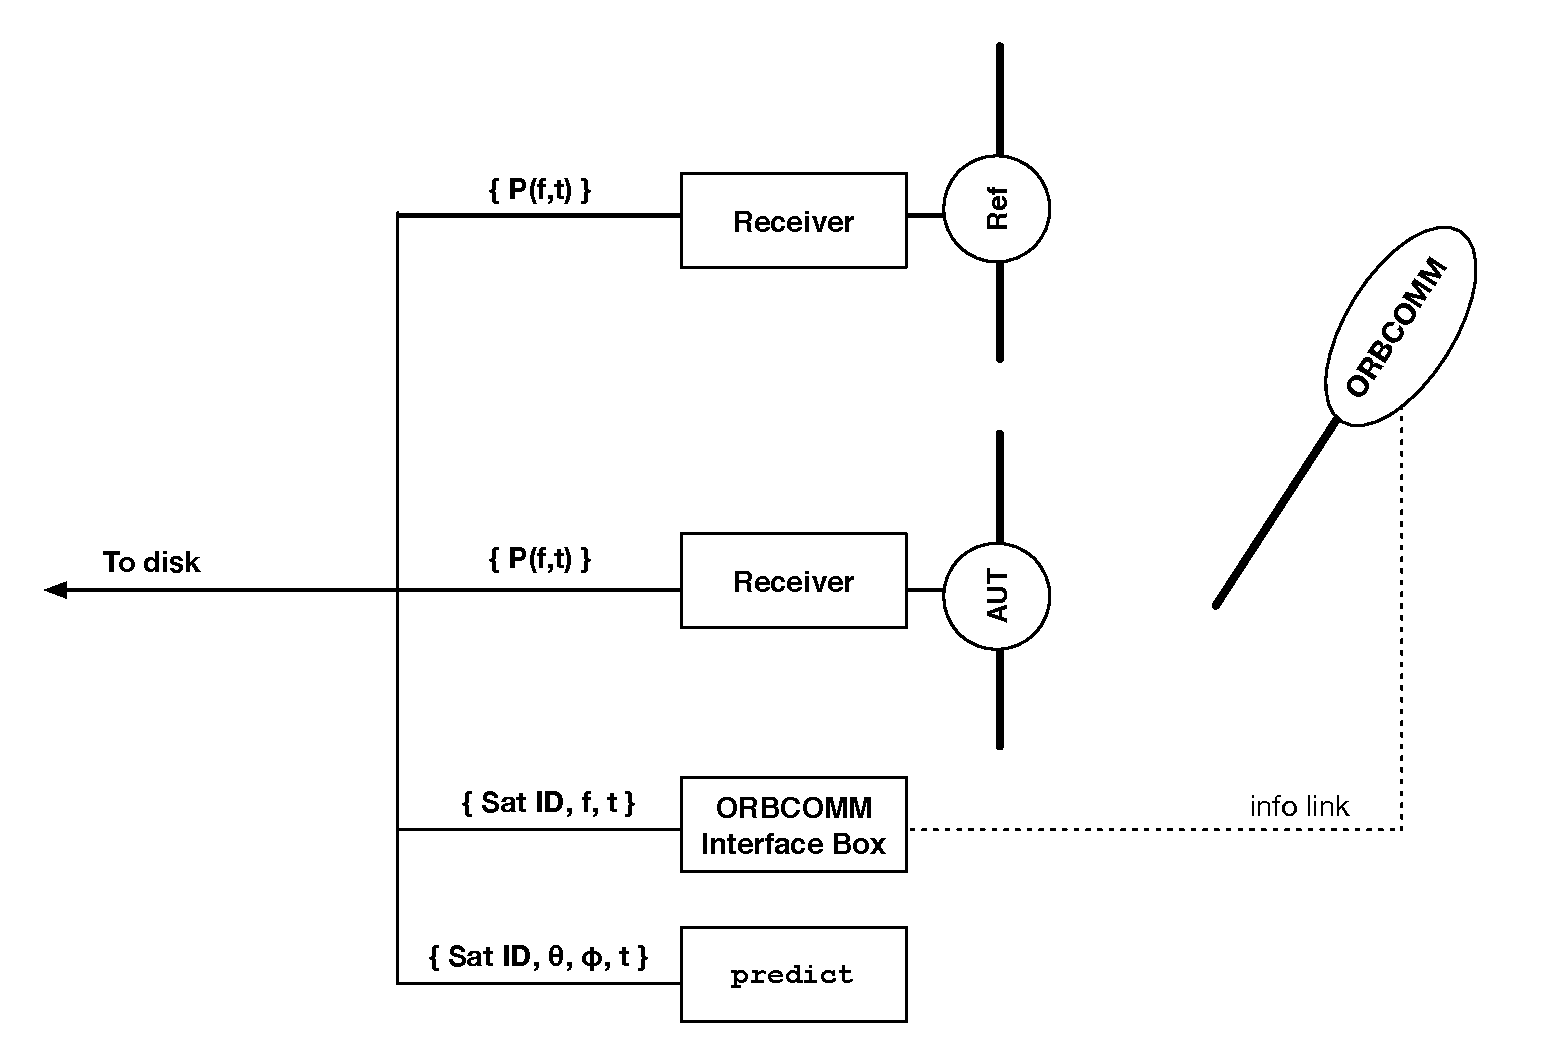
\includegraphics[width=7in]{chap1_precision_beammapping_figures/system_overview_diagram.pdf}
\caption[Simplified diagram of our beam measurement system and data flow.]{Simplified diagram of our beam measurement system and data flow. ORBCOMM satellite signals are received by our Reference Antenna and the AUT, each passing through the receiver chain described in Sec. \ref{sec:measurementsystem} which outputs a power spectrum with 2 kHz resolution between 137--138 MHz every $\sim$200 ms. At each time step, a copy of {\tt predict} running on our data acquisition computer outputs the positions and IDs of all ORBCOMM satellites above the horizon, while transmission frequencies are logged by our ORBCOMM Interface box. }
\label{fig:systemoverviewdiagram}
\end{figure}

This work was performed at the National Radio Astronomy Observatory site in Green Bank, West Virginia, located in the US National Radio Quiet Zone. Though the ORBCOMM satellites dominate the radio sky in the 137--138 MHz band, wide band interference from terrestrial radio transmitters causes saturation problems in other geographic locations. Our AUT and reference antenna are positioned 50m apart on a North-South baseline located at (38.429348$^\circ$N, -79.845737$^\circ$E), and aligned to an accuracy of about a degree, as confirmed by Google Earth (http://www.google.com/earth) imagery. The Green Bank site is not perfect, however, and the surrounding hills and radio telescopes raise concerns of  shadowing and multipath effects. We assess these with a null experiment in which the beampattern of a known reference-style dipole is used as the AUT (see Section \ref{sec:nullexpt}).

In this work we measure the angular response of each instrumental polarization (NS and EW) to unpolarized radiation, leaving for future work measurement of the full polarized beampatterns. While it is not obvious that fully polarized satellite probe signals suffice to measure unpolarized beampatterns, we show in Appendix \ref{sec:measurementappendix} that this is in fact possible if both our reference antenna and our AUT have the same polarization response. 

\subsection{ORBCOMM Satellite Constellation}
\label{sec:orbcomms}

ORBCOMM Inc. operates a constellation of $\sim30$ communications satellites in low Earth orbit (altitude $\sim800$km) designed for users requiring low baud rate communication with remote sites. The satellites provide excellent Earth-coverage and near continuous transmission, predominantly occupying orbital planes with inclinations between $\pm45^\circ$ and 10 narrow ($\sim20$ kHz wide) subbands in the 137--138 MHz band. An advantage of these satellites over higher altitude satellites (such as the GPS constellation) for beampattern measurements is that good sky coverage is achieved far more quickly due to the shorter orbital period and rapid orbital precession resulting from the lower altitude. In particular, sky coverage at our Green Bank site is limited only by absence of satellites with inclinations greater than $45^\circ$. The information content of the transmitted satellite signals is irrelevant for our purpose and is lost in the RMS power measurements of our data acquisition system (see Section \ref{sec:daq}). 

Each satellite's frequency is relatively stable over days, but shifts periodically to avoid interference within the constellation. There are typically several ORBCOMM satellites above the horizon at any given time, and while we can easily compute their positions using published orbital elements, we must determine which frequencies correspond to which satellites. \citet{zheng14} use interferometric phases to identify and exclude times when more than one satellite is present. We are able to take advantage of \textit{all} satellite passes using an ORBCOMM User Interface Box (typically provided by ORBCOMM Inc. to users) connected to a separate antenna, whose debug port logs the satellite number and frequency band occupied by each passing satellite. 

During data collection, we record the satellite positions using the Linux program {\tt predict}\footnote{http://www.qsl.net/kd2bd/predict.html} which numerically integrates the orbits using orbital elements (TLE) data published by Celestrak\footnote{http://www.celestrak.com/NORAD/elements/orbcomm.txt} daily. We run two copies of {\tt predict} in live multi-satellite tracking mode on our data acquisition (DAQ) computer, and query them for the angular positions of all satellites currently above the horizon whenever a satellite power measurement is made (typically every 200ms). We save this information with the recorded satellite power data. See Section \ref{sec:daq} for a detailed description of our data acquisition system.

\subsection{Reference Antenna}
\label{sec:refant}
Our reference antenna is a simple dual-polarization dipole mounted above a 2 m $\times$ 2 m ground plane, elevated 48.3 cm above the soil (see left panel of Figure \ref{fig:antennas}). The antenna itself is made from 90.4 cm long and 0.5 inch diameter copper tubing, and is encapsulated in 2 in diameter Schedule 40 PVC tubing. The beampattern of the dipole was derived from an electromagnetic analysis of the physical structure over a finite ground plane using CST Microwave Studio (https://www.cst.com/Products/CSTMWS). The soil is modeled as a cube of lossy dielectric 3.05 m on a side having a relative permittivity of 13 and electrical conductivity of 0.005 S/m. 

\begin{figure}
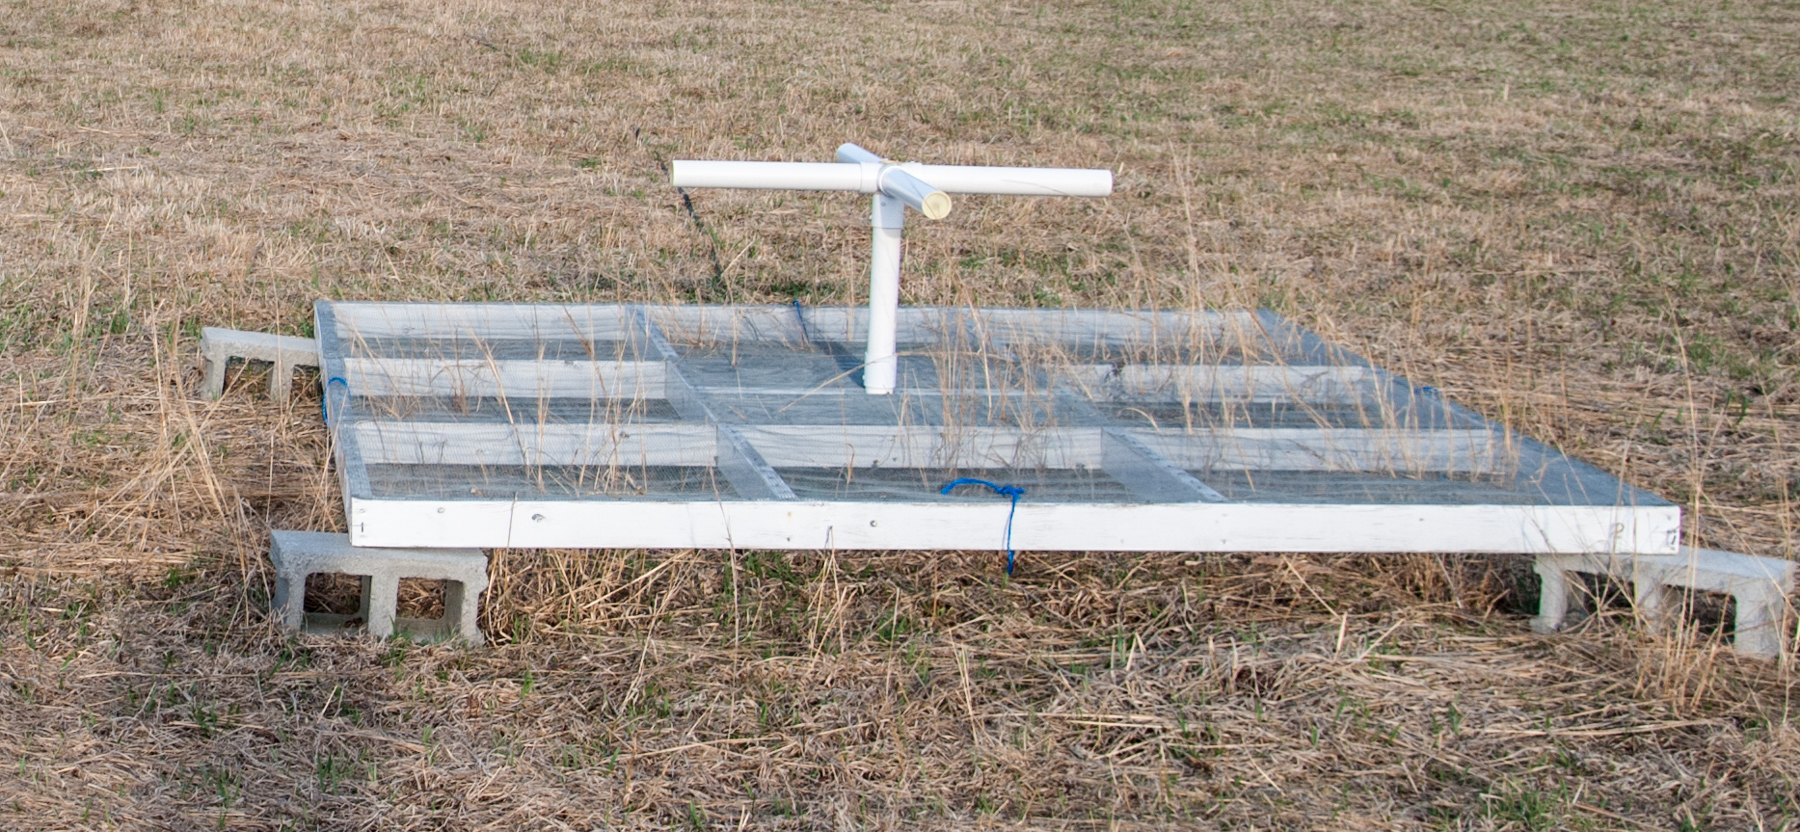
\includegraphics[height=1.5in]{chap1_precision_beammapping_figures/ref_ant.jpg}
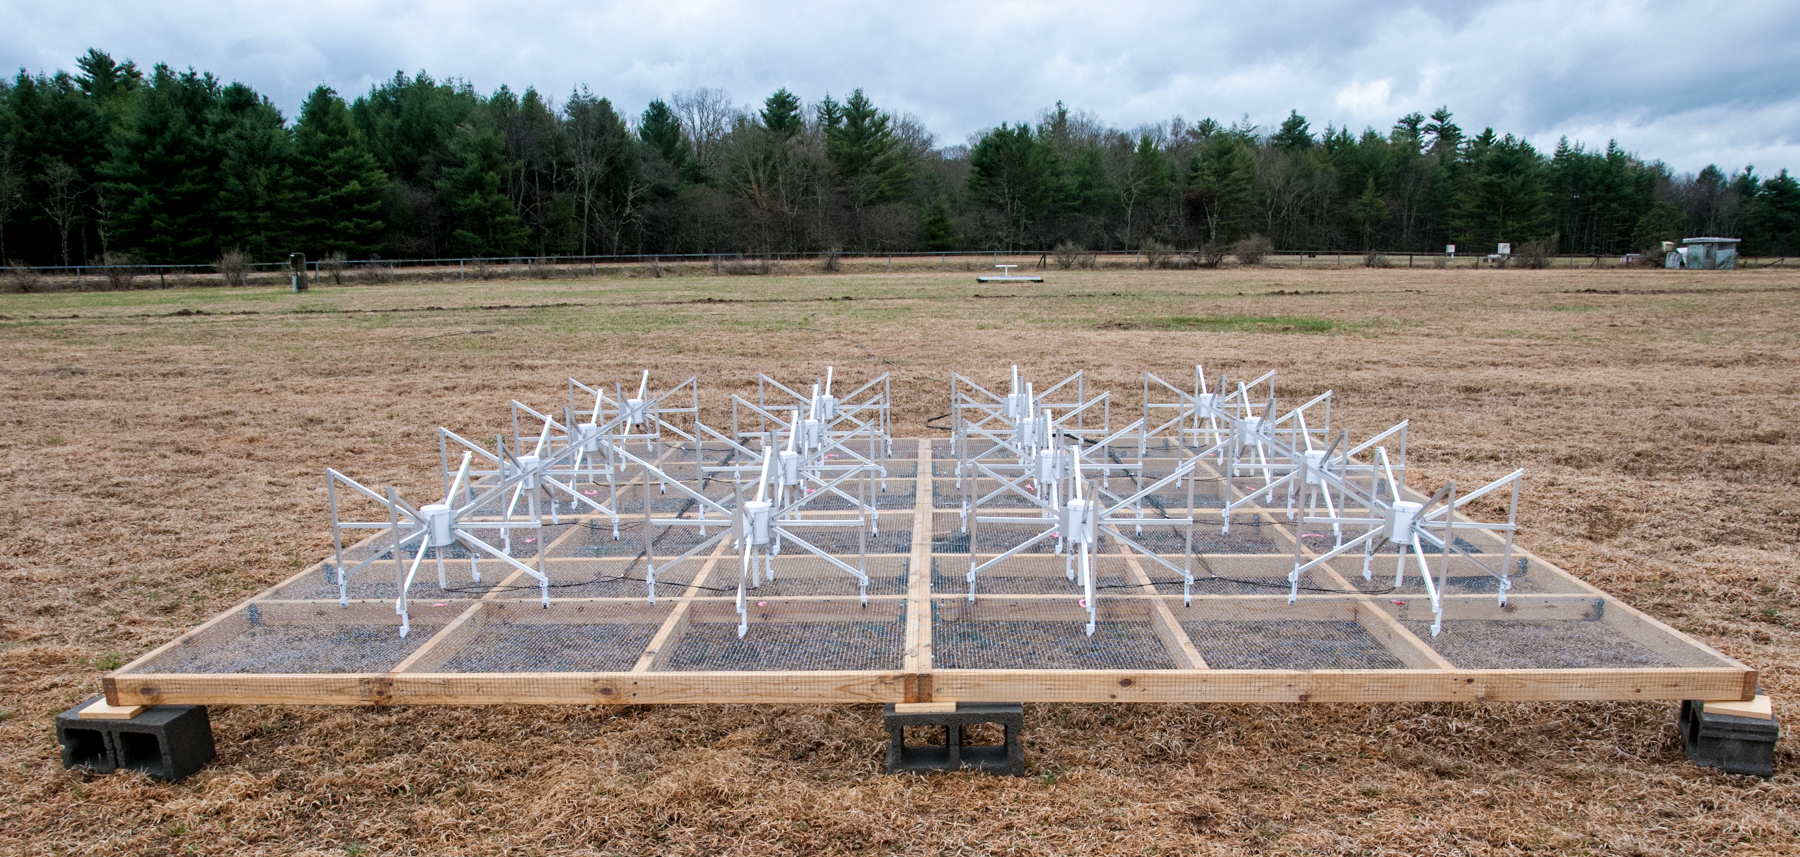
\includegraphics[height=1.5in]{chap1_precision_beammapping_figures/apr14tile.jpg}
\caption[Photos of our reference antenna (left) and the MWA tile (right)]{Reference antenna on 2 m $\times$ 2 m ground screen (left) (see Section \ref{sec:refant}) and MWA antenna tile on 5 m $\times$ 5 m ground screen (right) (see Section \ref{sec:mwatile}) deployed at the National Radio Astronomy Observatory--Green Bank.}
\label{fig:antennas} 
\end{figure}

\subsection{Data Acquisition Hardware}
\label{sec:daq}

Our receiver produces a mean power measurement in each frequency channel in each of two instrument polarizations (NS and EW) for each of our two antennas (the AUT and the reference antenna) every $\sim$200 ms. The raw signals are first mixed with a 127 MHz local oscillator down to an intermediate frequency of $\sim$10.5 MHz, then simultaneously sampled at 2 MHz, digitally mixing them down to the 0--1 MHz baseband (i.e. one of the Nyquist zones falls in the frequency range 0--1 MHz).  A 12-bit ADC acquires a burst of 51,200 samples on which 50 FFTs of length 1024 samples are performed, effectively covering the 137--138 MHz bandwidth with a resolution 2 kHz (cf. $\sim$20 kHz bandwidths of ORBCOMMS). From these measured voltage Fourier amplitudes $\widetilde{V}_{\mathrm{ant},\mathrm{pol},i}(f)$, where $i$ runs from 1 to 50, the RMS powers $\langle|\widetilde{V}_{\mathrm{ant},\mathrm{pol},i}(f)|^2\rangle_i$ are saved to disk for each antenna, polarization, and frequency channel along with a list of all satellites currently above the horizon and their angular positions (obtained from {\tt predict}, see Section \ref{sec:orbcomms}). A full complex polarization analysis of the AUT beam would be possible given measurements of voltage cross powers $\langle \widetilde{V}_{\mathrm{ant},\mathrm{pol},i}(f)\widetilde{V}_{\mathrm{ant'},\mathrm{pol'},i}^*(f)\rangle_i$, though this places stringent requirements on instrumental phase stability and we thus reserve it for future work.

\section{Data Analysis}
\label{sec:analysis}
\subsection{Processing Satellite Passes}
\label{sec:processingsatellitepasses}
The first step is to determine each satellite's transmission frequency during each pass. We have developed a script to extract this information from the captured debug output of the ORBCOMM User Interface Box, which periodically ``syncs'' with passing satellites and logs their identifiers and transmission frequencies. We assume a time window of 30 minutes over which the recorded frequencies are valid, and use this mapping of satellites and time windows in the next step of the analysis.

Next, we manipulate the satellite power data. At each $\sim$200 ms time step, a beam measurement can be made at the position of each satellite above the horizon (each of which is transmitting on a different, but now known frequency). This is done separately for EW and NS instrumental polarizations. The measured AUT and reference dipole powers in each satellite's frequency band are determined by integrating the measured RMS band powers over the central 15 kHz of the satellite's signal band. The background power level is estimated as the minimum of the received power level at start and end of each pass (when the satellite is below the horizon), and data within 20 dB of that floor are rejected. This ensures that the bias on measured beampattern due to the sky noise is less than 1\%. 

As a heuristic description of our measurements assuming the satellite signals are unpolarized, consider the received powers by the AUT and the reference antenna, $P_\mathrm{AUT}$ and $P_\mathrm{ref}$, in one instrumental polarization, and let $B_\mathrm{ref}$ and $B_\mathrm{AUT}$ be their unpolarized beam responses at the angular position of the satellite. Let $F$ be the incident flux from the satellite so that $P_\mathrm{ref}=B_\mathrm{ref}F$ and $P_\mathrm{AUT}=B_\mathrm{AUT}F$. Then it is clear than the AUT beam response in the satellite direction is given by

 \begin{equation}
\label{eqn:beammeasurement}
B_\mathrm{AUT}=P_\mathrm{AUT}B_\mathrm{ref}/P_\mathrm{ref}
\end{equation}

This is essentially our analysis, done separately for EW and NS oriented antennas. We show in Appendix \ref{sec:measurementappendix} that the polarization of satellite signals does not affect Equation \ref{eqn:beammeasurement}, assuming both antennas have the same polarization response.

\subsection{Forming Power Patterns}
\label{sec:formingpowerpatterns}

To form power patterns, we grid the measured AUT beam values from many satellite passes into equal solid angle cells on the sky using the HEALPix software package \citep{healpix} to (1) facilitate comparison with model power patterns; (2) average over short-timescale fluctuations due to noise and multipath effects; and (3) facilitate rejection of outliers in each sky pixel due to rare saturation issues. We choose a cell size of 1.8 deg (nside=32) which results in $\sim$5 satellite passes and $\sim75$ measurements in each pixel per day, out of which $\sim5$ typically fall outside of the central 90\% and are rejected as outliers. This results in few percent precision on our measured beams and sufficient resolution to resolve features of interest except within several degrees of the the MWA beam nulls, where the beam changes on sub-pixel scales.  Normalizing the measured beam might be done by rescaling it to peak at unity, though we opt for a less noisy normalization by fitting for a rescale factor to best match the measured beam to the normalized analytic model within $\sim10$ degrees of boresight. 

\subsection{Assessing Systematics with a Null Experiment}
\label{sec:nullexpt}

We characterize systematics using a null experiment, in which we use a second reference-style antenna as the AUT. The beampatterns of the two reference antennas will deviate from each other due to environmental effects (e.g., multipath effects or shadowing) and instrumental non-idealities (e.g., alignment errors or imperfections in the ground screen, soil, or dipole itself). Our null experiment will effectively measure the ratio of these two antenna beampatterns, and thus, the level at which they deviate from each other. We interpret this measure as a rough proxy for deviation of each antenna away from the ideal electromagnetic model.

Figure \ref{fig:satellitepass} shows a satellite pass from this setup in detail. Over the course of 15 minutes, the satellite rises out of the background, passes through the visible sky, and falls below again (shown in the top panel). The units are dB relative to the background level (shown below to be predominately diffuse galactic emission), and we mark with vertical lines the region within which the received power is more than 20 dB stronger than the background. If the AUT beampattern is different from that of the reference dipole, beam measurements outside this region will suffer systematics at a level of a few percent and larger due to the diffuse galactic emission received in addition to that from the satellite. We opt to simply avoid this region in lieu of subtracting a background model. The ratio of the two reference antenna powers (shown in the middle panel) is mostly consistent with unity up to $0.5-1$ dB statistical scatter, systematic biases of comparable magnitudes are apparent at large zenith angles. As this is just one satellite pass, it is difficult to draw general conclusions about which regions of the sky are least or most susceptible to such biases. Only after gridding many satellite passes together does a fuller picture emerge. Note, though, that given the brightness of the ORBCOMM satellites and the averaging discussed in \ref{sec:formingpowerpatterns}, we interpret the statistical fluctuations as a combination of multipath reflections (different at the two antenna locations) and polarization mismatch, not as receiver noise. 

\begin{figure}
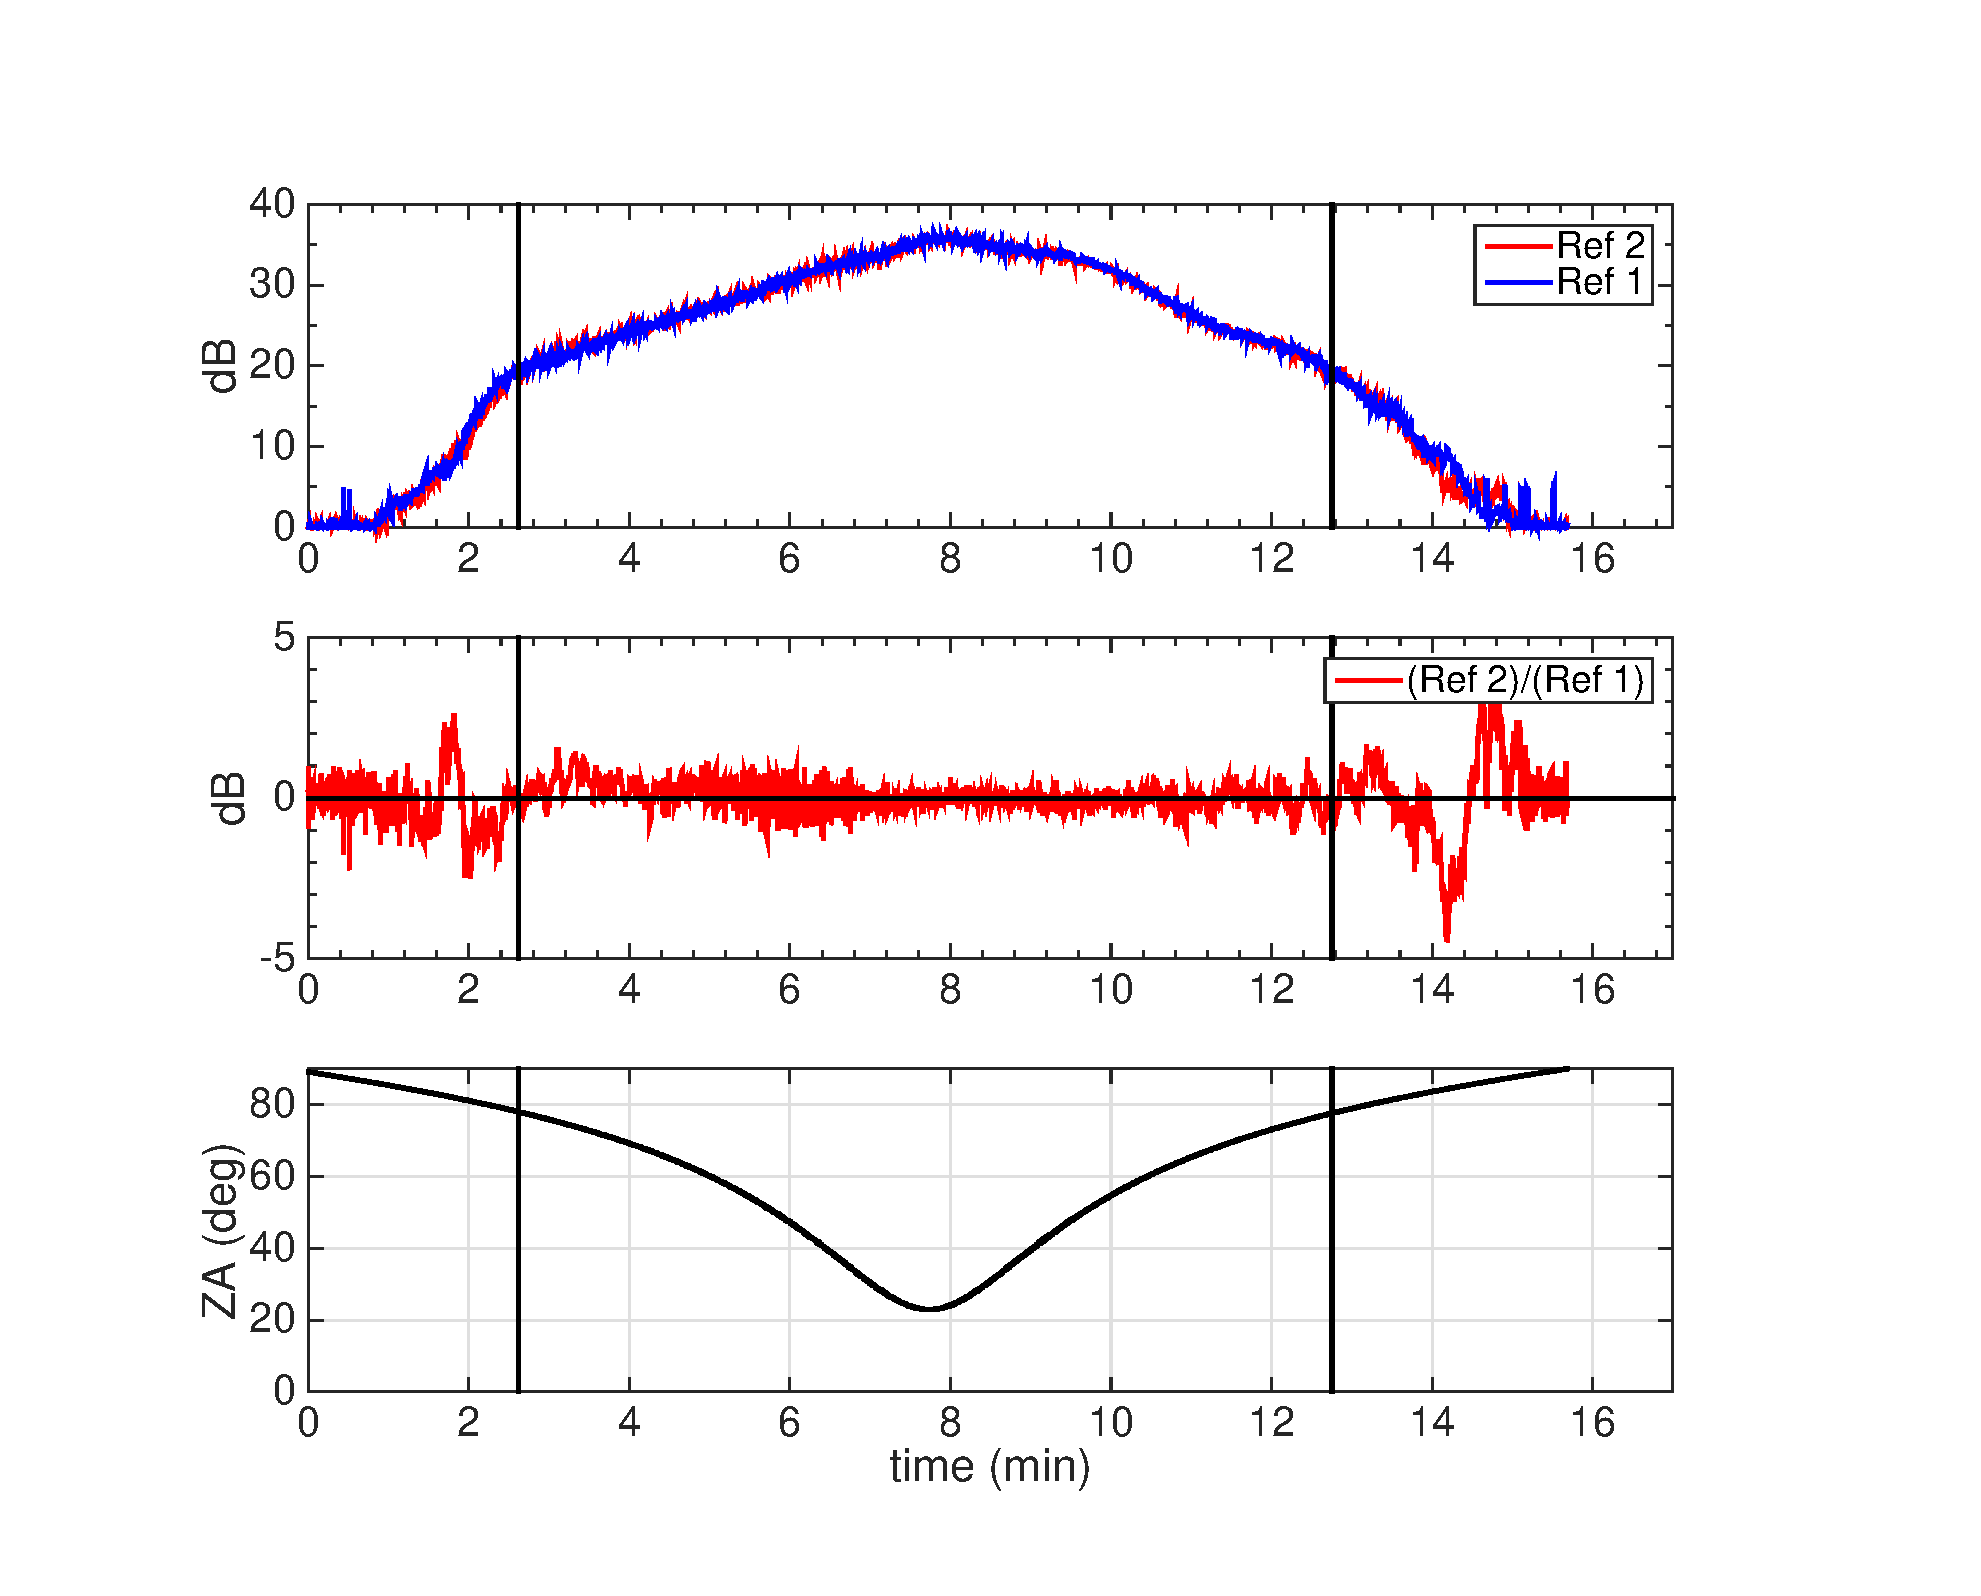
\includegraphics[width=6.5in]{chap1_precision_beammapping_figures/null2sat23_pass75332.eps}
\caption[Analysis of a typical satellite pass from our null experiment.]{Analysis of a typical satellite pass from our null experiment, in which the AUT is replaced by a reference-style antenna. The satellite rises out of the galactic background power (see Fig. \ref{fig:skynoise}), passes high in the sky, then drops below the horizon over the course of roughly 15 minutes (top panel). Both curves are in units of dB relative to the background level estimated at the beginning of the pass. Outside the region enclosed by vertical lines, the signal to background ratio is smaller than 20 dB, meaning that the satellite signal received by each antenna is corrupted at the few percent and larger level by diffuse galactic power.  The fluctuations in the ratio of the two antenna responses (middle panel) are typically at the $\pm0.5$dB level  and are due to multipath reflections and polarization mismatch, not receiver noise. We also plot the satellite zenith angle (bottom).}
\label{fig:satellitepass}
\end{figure}


To characterize the behavior of these fluctuations as they manifest in power patterns, we combine 296 satellite passes in the null experiment configuration recorded over 32 hours (spread over 4 days) into a measured beampattern of the reference antenna (Figure \ref{fig:null2map}). The measured reference antenna beampattern is consistent with our numerical model within few percent statistical scatter within 20 degrees of zenith, and shows modest systematic trends at the 10\% level farther out suggestive of a few degree rotational misalignment. This level of agreement sets an upper limit on beam measurement systematics due to environmental effects and instrumental non-idealities as discussed above. We thus interpret these results as measurements of the accuracy and precision of our beam measurement system in its current configuration. In Sec. \ref{sec:discussion}, we discuss approaches to mitigating these systematics further.

\begin{figure}
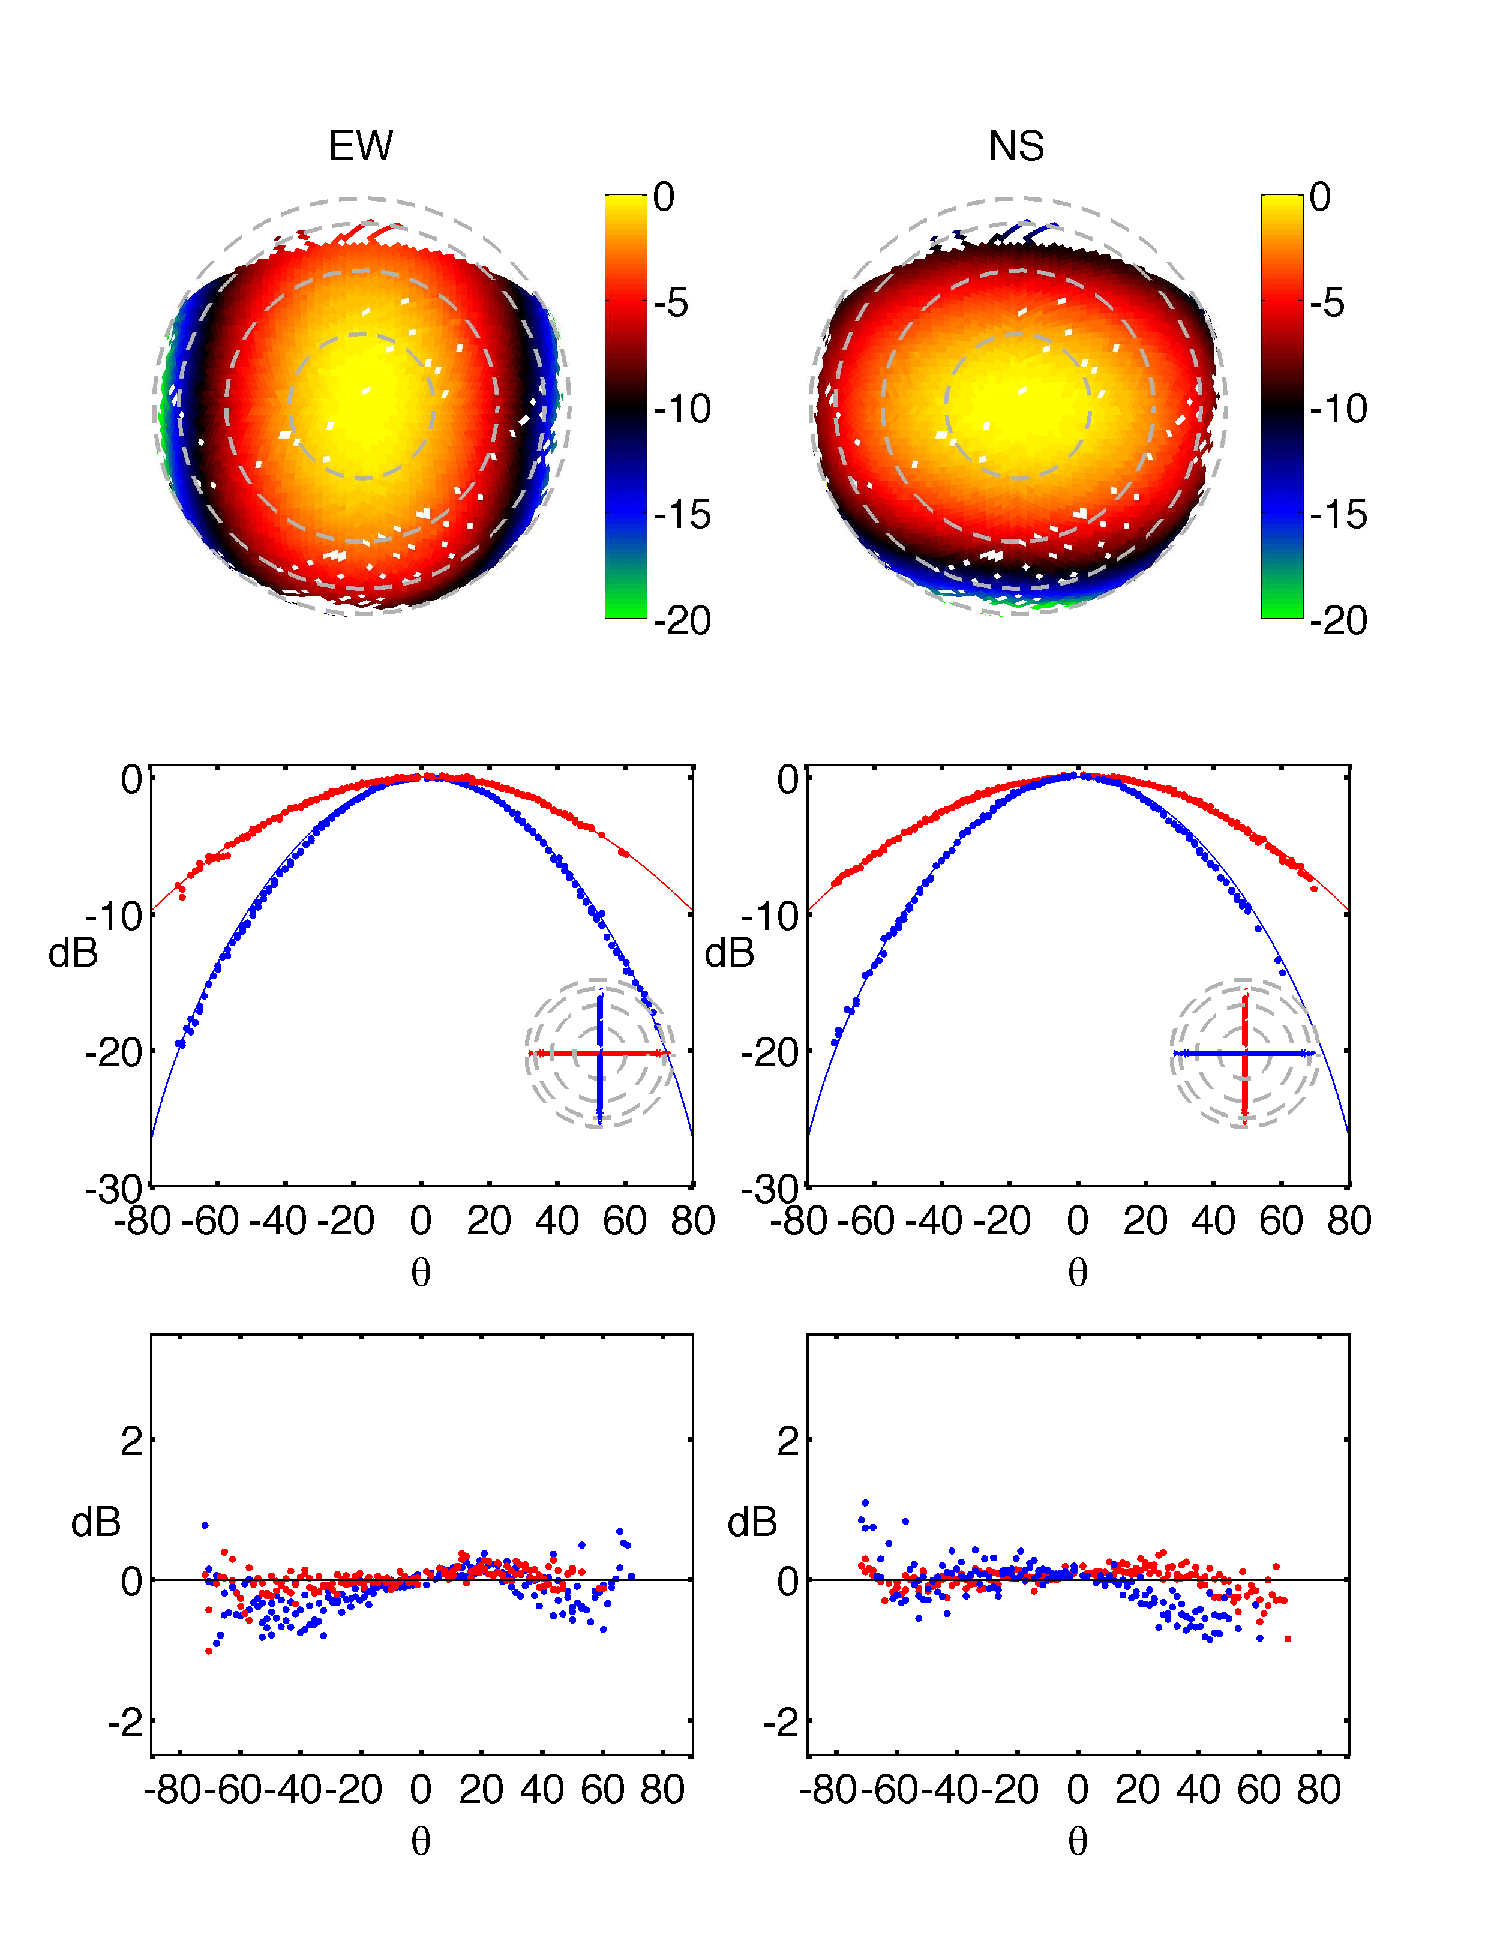
\includegraphics[width=5in]{chap1_precision_beammapping_figures/null2_abs.pdf}
\caption[Results from our null experiment.]{Results from our null experiment in which the AUT is another reference antenna. Beams of the EW (NS) oriented dipoles are shown in the left (right) column. The measured AUT beampattern is plotted in dB relative to its boresight gain (top). These maps are in sine projection with North at the top and East at the right. Dashed circles mark 20, 40, 60, and 80 degrees from zenith. We also show measured and model beampatterns (middle) and deviations from the model (bottom) on slices through the E (red) and H (blue) antenna planes.}
\label{fig:null2map}
\end{figure}


As a check on the reliability of our background estimation (used only to identify and avoid times of significant background power relative to satellite power), we plot in Figure \ref{fig:skynoise} the observed background level as a function of time versus that predicted from the Global Sky Model (de Oliveira Costa 2008) and our model reference antenna beampattern. Even neglecting the sun, the observed background estimates agree qualitatively with the GSM at the $\pm0.5$ dB level, close to its stated accuracy of $\pm10\%$. Note that slight phase and amplitude disagreements at this level are expected as the GSM is generated through interpolation between sky maps at other frequencies, and errors are thus correlated over large scales. That the observed background levels are  roughly consistent with the predicted galaxy power demonstrates that the ORBCOMM satellites are spaced sufficiently far apart in their orbits and frequency bands so as to not overlap in time, which is crucial for our experiment.

\begin{figure}
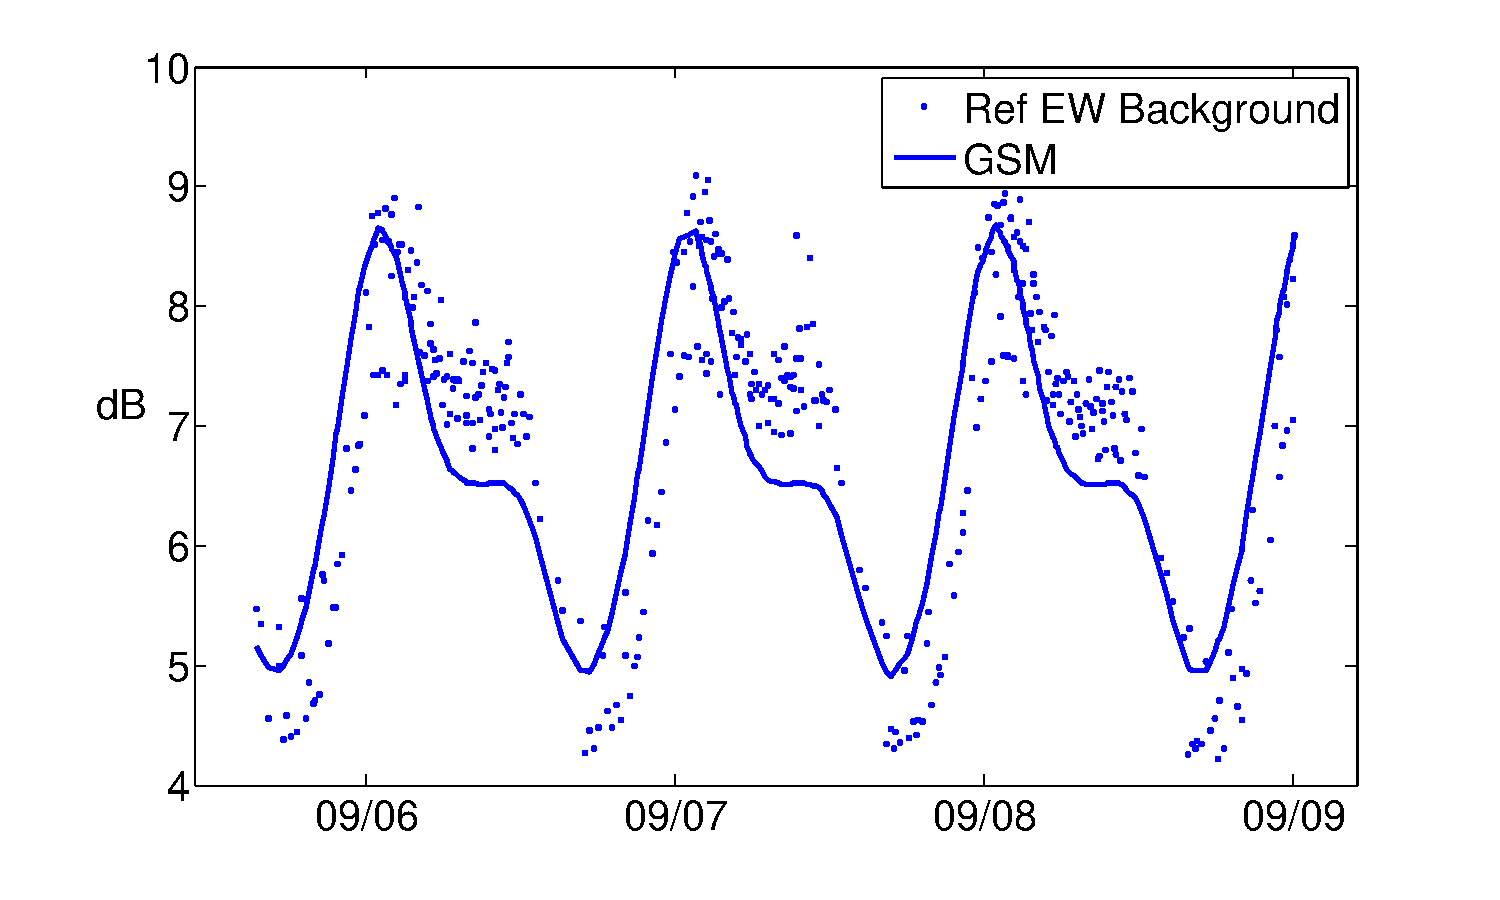
\includegraphics[width=5in]{chap1_precision_beammapping_figures/skynoise_null2.pdf}
\caption[Observed reference antenna background levels.]{Observed reference antenna background levels measured at the beginning or end of each satellite pass, plotted with a model time-dependent background computed from the Global Sky Model (GSM) \citep{gsm} and the model reference antenna beampattern. The data agree with the GSM model given its stated $\pm10$\% accuracy.}
\label{fig:skynoise}
\end{figure}

\section{MWA Antenna Tile}
\label{sec:mwatile}

Having quantified the accuracy and precision of our setup, we proceed to a study of the beampattern of an MWA antenna tile (hereafter MWA tile). The MWA tile consists of a 4$\times$4 grid of dual-polarization bowtie dipoles whose signals are combined in a delay-line beamformer. The dipoles are vertical bowties with dimensions 74 cm across and 84 cm on the diagonal, optimized to have a broad frequency response in the 100--200 MHz band. They are mounted on a 5 m $\times$ 5 m ground screen attached to a leveled wooden frame approximately 20 cm above the ground. The center-to-center dipole spacing is  1.1m and the center-to-ground-screen distance is 30 cm. For this experiment, we construct the ground screen out of 5 pieces of wire mesh (19 gauge, 0.5'' spacing) which are crimped together every 5 inches to form a constant potential surface connected to earth ground. Each dipole has a 20 dB LNA with integrated balun. The beamformer sums 16 dipole signals for each of the two polarizations (NS and EW), producing a beam with Full-Width-at-Half-Maximum (FWHM) $\sim23^\circ$ at 137 MHz, with sidelobes at the $-20$ dB level. By digitally engaging delay lines in increments of $\sim$450 ps to each signal pathway, the beam may be steered far from zenith. The delays are engaged through simple digital control with no amplitude or phase calibration needed. Slight deviation from perfect gain and delay matching (see Sec. 4.3) across the beamformer pathways is one of the mismodeling effects this work will probe. Lastly, we note that beamformer adds 30 dB of gain to the summed signal, to which we add 36 dB of attenuation to avoid saturating the ADC in our receiver. 

\subsection{Model Beampatterns}
\label{sec:modelbeampatterns}

As 137 MHz is well below the half wavelength frequencies of the characteristic lengths of the MWA Dipole (202 MHz and 178 MHz), the Hertzian dipole model is expected to be valid, though deviations near the sidelobes would not be unexpected. The phased array and ground screen factors of the MWA tile are encapsulated in the array factor $\textbf{A}_{11}(\theta,\phi)=\textbf{A}_{22}(\theta,\phi+\pi/2)$ (see Appendix A),
\begin{equation}
\label{eqn:tilemodel}
|\textbf{A}_{11}(\theta,\phi)|^2 \propto \sin^2\left(kh\cos\theta\right)\left|\sum_{i=1}^{16}e^{i (\vec{k}\cdot \vec{x}_i+\eta_i)}\right|^2
\end{equation}
Here $h=0.3$ m is the height of the dipole midpoints off the ground screen, $\vec{k}$ is the direction of the satellite, $\eta_i$ is the phase delay applied by the beamformer, and $\vec{x_i}$ is the position of antenna $i$ on the grid in the $xy$ plane. The phase delay can be expressed as $\eta_i=2\pi fd_i\times$(435 ps) where $d_i$ is an integer between 0 and 31 which is specified when controlling the beamformer. Lastly, we use coordinates where $\hat{x}$ points towards the East, $\hat{y}$ points towards the North, and $\hat{z}$ points towards Zenith, and $\vec{k}=\frac{2\pi}{\lambda}(\sin\theta\sin\phi\hat{x}+\sin\theta\cos\phi\hat{y}+\cos\theta\hat{z})$. Combining Equations \ref{eqn:tilemodel}, \ref{eqn:rotmat}, and \ref{eqn:autbeam} gives our analytic MWA tile model. 

We also compare our measurements to the more advanced beam model presented by \citet{sutinjo2015} which includes dipole-dipole coupling effects and a numerical dipole model on realistically modeled soil. We use their average embedded element model, as work on a full electromagnetic coupling model is ongoing. Below $\sim180$ MHz, the corrections due to dipole coupling effects are small within the main lobe, but potentially observable in beam measurement extending into the sidelobes, like ours.

\subsection{Beampattern Measurements}

Figure \ref{fig:zenithtilemap} shows our measured MWA tile beampattern (top panel) when pointed towards zenith, constructed from $\sim$400 satellite passes recorded over $\sim$4 days. The beam is plotted on the HEALPIX grid discussed in Sec. \ref{sec:formingpowerpatterns}. We also plot the measured beampattern and our analytic model on slices through these polar plots on the E and H (red and blue, respectively) antenna planes (middle panel), as well as the ratio of measured over analytic model beams (bottom panel). The numerical model of \citet{sutinjo2015} is plotted relative to the analytic model in the bottom panel for comparison (dashed lines), and should align with the data points if it explains the observed deviations. While measured beampatterns are often compared with models in simple beam sensitivity \textit{difference} plots, we view \textit{ratio} plots (i.e., differences of dB quantities) as more relevant given that primary beam sky weighting during both calibration and primary beam correction are multiplicative operations. Ratio plots also highlight the off-zenith regions where beams are typically most poorly modeled, the regions where foregrounds are most at risk of affecting EOR science, as discussed in Sec. 1.

\begin{figure}
\includegraphics[width=5in]{chap1_precision_beammapping_figures/Zenith_abs.eps}
\caption[Measured MWA tile beampattern for the zenith pointing.]{The measured MWA tile beampattern for the zenith pointing is plotted in dB relative to its boresight gain (top). Beams of the EW (NS) oriented antennas are shown in the left (right) column. The maps are in sine projection with North at the top and East at the right. Dashed circles mark 20, 40, 60, and 80 degrees from zenith. We show measured and model beampatterns (middle) and deviations from the model (bottom) on slices through the E (red) and H (blue) antenna planes. Dashed lines in the bottom panel show the model of \citet{sutinjo2015} relative to the analytic model. Vertical dotted lines mark the model FWHM of $\sim$23 degrees at 137 MHz.}
\label{fig:zenithtilemap}
\end{figure}

Within the half power point ($\sim$12 degrees away from zenith) we observe agreement with our analytic model beam pattern within $\sim$5\% statistical fluctuations. Beyond that zenith angle, towards the edges of the main lobe and in the few percent sidelobes, we observe systematic deviations away from the model at the dB level. We discuss these deviations and their patterns further in Sec. \ref{sec:mwaerrors}. Both positive and negative trends are observed.

We have also measured the MWA tile power pattern at several off-zenith pointings, two of which are shown in Figures \ref{fig:E03S00tilemap} (20 degrees East) and \ref{fig:W03S00tilemap} (20 degrees West). For these pointings, the direction of boresight is not in the E and H antenna planes, so we instead rotate the antenna E and H planes to the boresight direction, yielding two orthogonal planes crossing the off-zenith main lobe. The level of deviation away from the model power patterns here is comparable with the Zenith pointing. 

\subsection{Error Analysis}
\label{sec:mwaerrors}

A detailed analysis of the causes and effects of beamforming errors in MWA tiles will be presented in a separate paper \citep{neben16}. In particular, that work is concerned with the finite precision of complex gain matching across the 16 beamformer signal paths (for each instrumental polarization) as well as tile rotation/tilt errors and dipole position errors. A budget of relevant systematics is established through laboratory measurements and compilation of manufacturer specifications and Monte Carlo simulations are run to propagate component uncertainties into direction-dependent beam power pattern uncertainties. Beam deviations at the level of 10--20\% are predicted in the sidelobes and near the edge of the main lobe, and significantly larger in the nulls. 

There are, however, several sources of error in the beam measurements presented in this work which are peculiar to our MWA tile at Green Bank. Our ground screen is elevated 20 cm off the ground on a wooden frame whereas the analytic and the cross-coupling models assume it is set on the ground. This is expected to affect the beam pattern at low elevations in particular, though in a symmetric manner. Non-coplanarity due to ground screen sag between its  frame supports also complicates the ground screen term in Eqn. \ref{eqn:tilemodel}, and may also introduce relative dipole tilts. Our ground screen is formed out of five rectangles of wire mesh, which are crimped together every 5". In contrast, the ground screen used in the deployed MWA tiles at the Murchison Radio Observatory in Western Australia are overlapped and welded, fixing a constant potential surface. 

Lastly slight tilts and rotations of our MWA tile due to our $\pm1.5^\circ$ alignment precision are larger than those affecting deployed MWA tiles. Such alignment errors are most prominent where the beam changes rapidly with angle as it does near the edges of the main lobe and in the sidelobes, and are difficult to correct for in our beam mapping experiment as they upset the polarization matching with the reference antenna. Numerical experiments suggest such alignment errors contribute systematics at the $\pm$20\% level.

Many of these errors will break the ideal symmetries of the tile beampatterns by introducing distortions and tilts of the main lobe and sidelobes, not unlike the patterns observed in the measured vs. model beam plots in Figures \ref{fig:zenithtilemap}, \ref{fig:E03S00tilemap}, \ref{fig:W03S00tilemap}. In particular, a slight main lobe widening is observed in the EW beams and a slight $\sim0.5^\circ$ tilt is observed in the NS beams. These discrepancies are observed across all three pointings, suggesting they are due to some combination of the tile non-idealities discussed above as opposed to per-pointing gain and delay errors in the beamformer.

\begin{figure}
\includegraphics[width=5in]{chap1_precision_beammapping_figures/E03S00_abs.eps}
\caption[The measured MWA tile beampattern for the 20 degree West pointing.]{Measured MWA tile power pattern for pointed 20 degrees West pointing. Same layout as Figure \ref{fig:zenithtilemap}, except here we plot beam slices through orthogonal planes through the main lobe (red and blue) which do not correspond to the E and H antenna planes because the direction of boresight is no longer in these planes.}
\label{fig:E03S00tilemap}
\end{figure}

\begin{figure}
\includegraphics[width=5in]{chap1_precision_beammapping_figures/W03S00_abs.eps}
\caption[The measured MWA tile beampattern for the 20 degree East pointing.]{Measured MWA tile power pattern for pointed 20 degrees East pointing. Same layout as Figure \ref{fig:E03S00tilemap}.}
\label{fig:W03S00tilemap}
\end{figure}


\section{Discussion}
\label{sec:discussion}

We have used the ORBCOMM satellite constellation to test of the feasibility of a sky transmitter-based beam measurement system for low frequency radio interferometers. Our system compares the power received by an AUT to that from a well-modeled reference dipole, whose ratio gives the relative beampattern of the AUT. The $\sim30$ ORBCOMM satellites provide sky coverage over two thirds of the visible sky from our Green Bank site in a single day, in part due to their low earth orbits and quick orbital precession. Their bright signals probe deep into antenna sidelobes, yielding measurements over 30 dB of MWA tile dynamic range, even after rejecting all data within 20 dB of the galactic noise background. This is an order of magnitude improvement in beam measurement depth over recent source-based beam measurements \citep{colegate14}.

We find through our null experiment that we are limited by 5\% statistical scatter within $20^\circ$ of zenith, and $10\%$ systematics farther out. We hope to definitively identify these fluctuations as multipath scattering in the future using multi-frequency probe signals to investigate their frequency dependence. The time scale of multipath fluctuations is set by the satellite's motion through the frequency-dependent interference pattern set up on the ground by nearby reflecting structures. Finer antenna alignment at the sub-degree level will also help mitigate systematics near the edges of the main lobe. 

We have used this prototype system to conduct the first measurements of an MWA tile beampattern over a large field of view including the main lobe and primary sidelobes. We find good agreement with a simple array factor-based short dipole model within the tile FWHM (23 degrees across at 137 MHz), but observe $\sim$ dB level systematic deviations towards the edge of the main lobe ($\theta\sim20^\circ$) and in the sidelobes. These deviations are larger than the $10\%$ systematics observed in our null experiment, and in principle represent the beam modeling errors we originally sought to measure. 

However, several considerations prevent our interpretation of these deviations as inherent in the MWA tile design, and thus representative of the 128 deployed antennas at the Murchison Radio Observatory in Western Australia. \citet{sutinjo2015} show MWA imaging results which are consistent with an advanced MWA tile model including mutual coupling, however our measured beampatterns appear no more consistent with this model than with our simple analytic one. Indeed the deviations we observe lack the symmetry expected from a beam modeling error due only to insufficiently precise modeling of the sort the cross coupling model is designed to correct. In that case, the zenith pointing EW and NS beampatterns should coincide after a $90^\circ$ rotation, and each should exhibit $180^\circ$ rotational symmetry. Additionally, as discussed in Sec. \ref{sec:mwaerrors}, known MWA beamforming errors are predicted to be at most $\sim20\%$ towards the edge of the main lobe and in sidelobes. However, there exist additional errors peculiar to our MWA tile set up in Green Bank which are more difficult to quantify (e.g., tile and dipole tilts, imperfect ground, ground screen sag, electric potential non-constancy). We thus view this work less as a measurement of \textit{the} MWA tile beampattern and more as a demonstration of the power of the ORBCOMM technique for identifying beam modeling errors (i.e., deviations of an as-built antenna from from its ideal model) down to the -30 dB level of the beam. We expect that further tests using probe signals from drones or multi-frequency satellites will both hone our understanding of the technique and set tighter constraints on beam models of the MWA tile.

Still unknown, though, are the effects of these errors on ongoing MWA Epoch of Reionization power spectrum measurements, which will depend both on their frequency dependence and the degree to which they limit calibration fidelity. This work has begun to probe these effects in a way that imaging cannot, as beamforming errors tend to average out when forming an image with many MWA tiles. However, such averaging of beamforming errors will be less perfect when forming sky power spectra because different antennas probe different regions of the $uv$ plane, depending on which baselines they are part of. Indeed as proposed by \citet{moralesandmatejek}, interferometric imaging algorithms taking per-antenna primary beams into account \citep{fhd, dillonmapmaking} may be critical in order to access the Epoch of Reionization.

\section{Appendix: Measurement of the unpolarized beampattern}
\label{sec:measurementappendix}

In general the response of an antenna to unpolarized radiation (e.g., thermal emission) is different from its response to polarized radiation (e.g., satellite signals). We show how the unpolarized beampattern (defined below) of the AUT may be measured despite any polarization of the satellite probe signal, assuming that both the AUT and the reference dipole have the same polarization response. 

In general, the voltage responses of these antennas to radiation from ($\theta,\phi$) relate to the two incident sky polarizations as

 \begin{eqnarray}
\vec{V}_\mathrm{AUT}&=&\textbf{A}\textbf{R}\vec{E}\label{eqn:measaut} \\
\vec{V}_\mathrm{ref}&=&\textbf{R}\vec{E}\label{eqn:measref}.
\end{eqnarray}

where $\vec{V}=\bigl(\begin{smallmatrix}V_x\\ V_y\end{smallmatrix} \bigr)$ and $\vec{E}=\bigl(\begin{smallmatrix}E_\theta \\ E_\phi\end{smallmatrix} \bigr)$. We use coordinates where $\hat{x}$ points to the East, and $\hat{y}$ points to the North. Spherical unit vectors $\hat{\theta}$ and $\hat{\phi}$ point in the directions of increasing $\theta$ and $\phi$, respectively. These unit vectors are thus functions of those angles, though here we consider radiation incident only from the single direction ($\theta,\phi$). Further, $\textbf{R}$ is a matrix which converts from sky polarization to instrument polarization and drops the $\hat{z}$ component (it is a subset of a rotation matrix),

\begin{equation}
\label{eqn:rotmat}
\textbf{R}=\left(\begin{array}{ccc}
\cos\theta\sin\phi & \cos\phi\\
\cos\theta\cos\phi & -\sin\phi
\end{array}\right).
\end{equation}


Assuming both antennas have the same polarization response, in the sense that the $\hat{x}$ ($\hat{y}$) oriented dipoles respond only to $\hat{x}$ ($\hat{y}$) polarized radiation, $\textbf{A}$ is a diagonal matrix which is a function only of angle on the sky and does not mix instrument polarizations. The physical origin of $\textbf{A}$ is the array factor of the MWA tile, as well as effects of ground screen, antenna geometry, and any dipole cross-coupling. In the ideal case, $\textbf{A}_{11}(\theta,\phi)=\textbf{A}_{22}(\theta,\phi+\pi/2)$, though our measurement does not assume this.

Consider the $\hat{x}$ oriented antennas as an example. The received powers in response to polarized radiation are
\begin{eqnarray}
P_\mathrm{AUT,x}&=& |\textbf{A}_{11}|^2|[R_{11}^2\langle|E_\theta|^2\rangle+2R_{11}R_{12}\Re\langle E_\theta E_\phi*\rangle +R_{12}^2\langle|E_\phi|^2\rangle]\label{eqn:poweraut} \\
P_\mathrm{ref,x}&=&R_{11}^2\langle|E_\theta|^2\rangle+2R_{11}R_{12}\Re\langle E_\theta E_\phi*\rangle+R_{12}^2\langle|E_\phi|^2\rangle.\label{eqn:powerref}
\end{eqnarray}


However, if the incident radiation is unpolarized with intensity $I$, then $E_\theta$ and $E_\phi$ are uncorrelated and equal in power and may be added together as powers to give the total received power ($I\equiv2\langle|E_\theta|^2\rangle=2\langle|E_\phi|^2\rangle$). The received powers are then
 \begin{eqnarray}
P_\mathrm{AUT,x}&=& |A_{11}|^2|(R_{11}^2+R_{12}^2)I/2 \\
P_\mathrm{ref,x}&=&(R_{11}^2+R_{12}^2)I/2,
\end{eqnarray}

and so the unpolarized $x$ beampatterns are given by
\begin{eqnarray}
B_\mathrm{AUT,x}&=& |A_{11}|^2|(R_{11}^2+R_{12}^2)/2\label{eqn:autbeam} \\
B_\mathrm{ref,x}&=&(R_{11}^2+R_{12}^2)/2\label{eqn:refbeam}.
\end{eqnarray}

To measure $B_\mathrm{AUT,x}$, we thus need only $A_{11}$, which can be computed from the ratio of $P_\mathrm{AUT,x}$ and $P_\mathrm{ref,x}$, as $\textbf{R}$ is known (see Eqns. \ref{eqn:poweraut} and \ref{eqn:powerref}). This is exactly the procedure outlined in Sec. \ref{sec:processingsatellitepasses}.  

\section{Acknowledgments}
This work was supported by NSF grant AST-0821321, the Marble Astrophysics Fund, and the MIT School of Science. We thank Pat Klima, Bang Dinh Nhan, and the staff at the National Radio Astronomy Observatory--Green Bank for assistance in setting up and debugging our experiment, and Haoxuan Zheng, Aaron Ewall-Wice, Josh Dillon, Lu Feng, and Daniel Jacobs for helpful discussions. We thank Nithyanandan Thyagarajan, Josh Dillon, Adrian Sutinjo, Tim Colegate, and the anonymous referees for very helpful comments on our manuscript.

This scientific work makes use of the Murchison Radio-astronomy Observatory, operated by CSIRO. We acknowledge the Wajarri Yamatji people as the traditional owners of the Observatory site. Support for the MWA comes from the U.S. National Science Foundation (grants AST-0457585, PHY-0835713, CAREER-0847753, and AST-0908884), the Australian Research Council (LIEF grants LE0775621 and LE0882938), the U.S. Air Force Office of Scientific Research (grant FA9550-0510247), and the Centre for All-sky Astrophysics (an Australian Research Council Centre of Excellence funded by grant CE110001020). Support is also provided by the Smithsonian Astrophysical Observatory, the MIT School of Science, the Raman Research Institute, the Australian National University, and the Victoria University of Wellington (via grant MED-E1799 from the New Zealand Ministry of Economic Development and an IBM Shared University Research Grant). The Australian Federal government provides additional support via the Commonwealth Scientific and Industrial Research Organisation (CSIRO), National Collaborative Research Infrastructure Strategy, Education Investment Fund, and the Australia India Strategic Research Fund, and Astronomy Australia Limited, under contract to Curtin University. We acknowledge the iVEC Petabyte Data Store, the Initiative in Innovative Computing and the CUDA Center for Excellence sponsored by NVIDIA at Harvard University, and the International Centre for Radio Astronomy Research (ICRAR), a Joint Venture of Curtin University and The University of Western Australia, funded by the Western Australian State government. Data on which figures and tables herein are based may be obtained by contacting the corresponding author Abraham Neben (abrahamn@mit.edu).


\chapter{Beamforming Errors in MWA Antenna Tiles and their Effects on EOR Science}
\label{chap:bferrors}

The content of this chapter was originally published as Neben, A.R. et al., \textit{Beamforming Errors in Murchison Widefield Array Phased Array Antennas and their effects on Epoch of Reionization Science}, ApJ, 820:44, 2016. Rich Bradley gave advice about how to mitigate RF coupling in precision laboratory delay measurements, but I did all the experimental work, analysis, and wrote the paper about our findings. Josh Dillon gave advice about how to assess the implications for foreground avoidance and subtraction techniques. \\

Accurate antenna beam models are critical for radio observations aiming to isolate the redshifted 21\,cm spectral line emission from the Dark Ages and the Epoch of Reionization and unlock the scientific potential of 21\,cm cosmology. Past work has focused on characterizing mean antenna beam models using either satellite signals or astronomical sources as calibrators, but antenna-to-antenna variation due to imperfect instrumentation has remained unexplored. We characterize this variation for the Murchison Widefield Array (MWA) through laboratory measurements and simulations, finding typical deviations of order $\pm10-20\%$ near the edges of the main lobe and in the sidelobes. We consider the ramifications of these results for image- and power spectrum-based science. In particular, we simulate visibilities measured by a 100\,m baseline and find that using an otherwise perfect foreground model, unmodeled beamforming errors severely limit foreground subtraction accuracy within the region of Fourier space contaminated by foreground emission (the ``wedge''). This region likely contains much of the cosmological signal, and accessing it will require measurement of per-antenna beam patterns. However, unmodeled beamforming errors do not contaminate the Fourier space region expected to be free of foreground contamination (the ``EOR window''), showing that foreground avoidance remains a viable strategy. 

\section{Introduction}

Efforts to observe the formation of the first galaxies during the Dark Ages and the subsequent Epoch of Reionization (EOR) are at the frontier of observational cosmology. Tomographic maps of neutral Hydrogen in the Intergalactic Medium at these redshifts, where the majority of the observable comoving volume of the Universe resides, will shed light on questions ranging from astrophysics and cosmology to particle physics (see \citet{FurlanettoReview, miguelreview, PritchardLoebReview, aviBook, zaroubi} for reviews). The extreme brightness temperature sensitivity needed to isolate this faint signal in the presence of bright galactic and extragalactic radio emission (foregrounds) and detector noise necessitates thousand-hour integrations and hundreds of antenna elements \citep[e.g.][]{parsons12b, beardsley13, nithya13, PoberNextGen}. This quest is highlighting characterization of antenna beam patterns, or primary beams, as crucial for high dynamic range calibration and foreground subtraction \citep{moore13, jacobs2013,nithya15,pober16}.

Two types of antenna mismodeling are relevant: (1) mismodeling of the mean antenna beam pattern; and (2) neglect of antenna-to-antenna variation. Both limit calibration and foreground subtraction fidelity in ways ranging from the obvious effect of subtracting sidelobe sources with the wrong apparent fluxes to the uncertain manner in which beam-related calibration errors average down with time. Indeed, modeling of antenna-to-antenna variation was long suspected to be critical for 21\,cm observatories, and early analysis pipeline development focused on incorporating knowledge of per-antenna beams in data reduction \citep{moralesandmatejek,fhd}, or even fitting for them in real time \citep{mwarts}.

The Murchison Widefield Array (MWA) \citep{lonsdale09,tingay13,mwascience} is now operating along with other instruments such as the Precision Array for Probing the Epoch of Reionization (PAPER) \citep{parsons14} and the LOw Frequency Array (LOFAR) \citep{lofar}. Analysis of the data from these arrays is bringing new urgency to the question of antenna beam patterns. Source-based methods have long been used to constrain the mean antenna beam using interferometer cross-correlations (visibilities) \citep[e.g.,][]{pober12, lofar,aavs}. More recently, working towards \textit{in-situ} measurements of per-antenna beams both for the MWA and for the developing next generation Hydrogen Epoch of Reionization Array (HERA) \citep{PoberNextGen,Whitepaper5}, \citet{neben15} present a beam measurement system using the ORBCOMM satellite constellation, an idea also explored by \citep{zheng14}. Development of a  drone equipped with a radio transmitter is also underway for the same application \citep{drone1,drone2,drone3}. 


\begin{figure}
%\centering
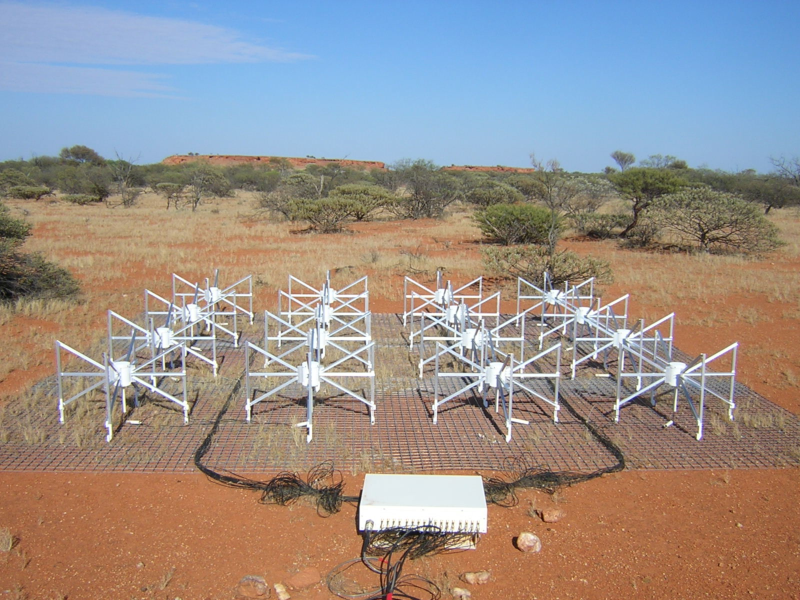
\includegraphics[width=8.38cm]{chap2_beamforming_errors/tile_photo.pdf}
\caption[A deployed MWA tile in the Murchison Radio Observatory.]{One of the 128 deployed MWA tiles in the Murchison Radio Observatory, Western Australia.}
\label{fig:tilephoto}
\end{figure}

As the MWA uses $4\times4$ phased arrays of bowtie dipoles (hereafter MWA tiles) as its fundamental antenna elements, it is more prone to antenna-to-antenna beam variation than experiments with simpler antenna elements. PAPER has opted for simpler dipole-style elements at the expense of 24\,dB less zenith gain and increased risk of contamination by RFI and galactic emission near the horizon \citep{nithya15}. The cost of the MWA's larger per-element collecting area is sensitivity to group delay and gain matching errors which disrupt the coherent addition of dipole signals\footnote{For instance, if two -20\,dB reflections create a signal which adds $\pi/2$ out of phase with the main signal, a phase error of  $\sim1$deg is created, equivalent to a delay of 20\,ps at 150\,MHz}. LOFAR has similarly opted for phased array antennas and is developing direction-dependent calibration techniques to counter these systematics \citep{lofareorpaper}, and the issue is of particular import for the low frequency Square Kilometer Array (SKA-Low) \citep{ska1,ska2,ska3} whose design relies heavily on beamforming. Unfortunately, adding extra parameters to the calibration model tends to increase noise and risks cosmological signal loss \citep[e.g.,][]{gmrtsignalloss}.

As a first step towards understanding the magnitude of these effects to guide development of solutions like satellite- and drone-based beam calibration schemes, we focus in this paper on characterizing these beamforming errors in MWA tile beam patterns and begin to study their effects in a 21\,cm power spectrum analysis. In Section 2 we discuss laboratory measurements of beamforming errors and other systematics affecting the MWA tile, and compile a budget of beamforming errors. In Section 3 we study the effects of these errors on mean and standard deviation beam patterns using simulations, and consider the implications for EOR power spectrum measurements in Section 5. We discuss our results in Section 6. In order to put these beamforming errors into context and understand their origin and the trade-offs made in designing the MWA tile, we elaborate in Appendix A on the summary of the MWA tile presented by \citet{tingay13}.

% description of the measurements
\section{Laboratory Measurements of Beamforming Errors}
\label{sec:measurements}

\subsection{Overview of Beamforming in the MWA}

 \begin{figure*}[t]
 \centering
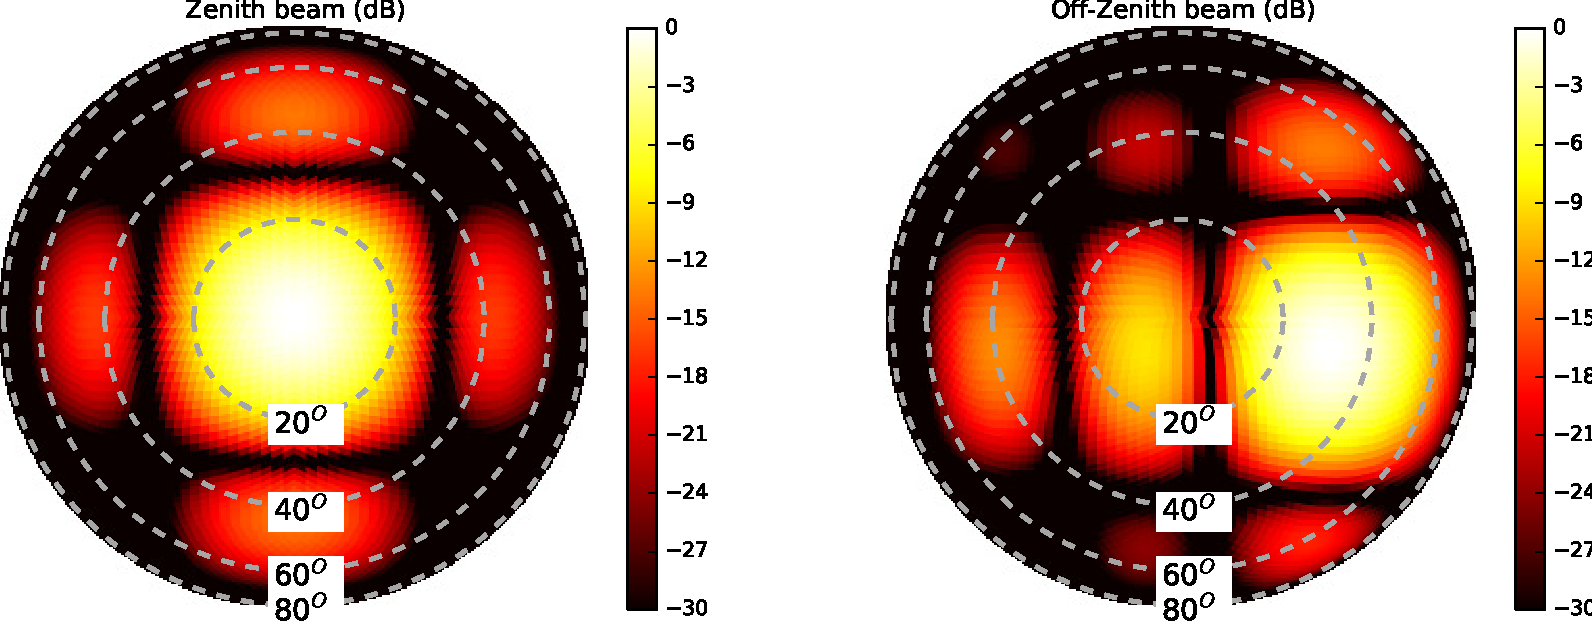
\includegraphics[height=2.5in]{chap2_beamforming_errors/zenith_and_offzenith_beams-eps-converted-to.pdf}
\caption[Ideal (no beamforming errors) beams for zenith (left) and off-zenith (right) pointings.]{Ideal (no beamforming errors) beams for a zenith pointing (left) and a representative off-zenith pointing (right) shown in sine-projection in units of dB at 150\,MHz. The off-zenith beam is pointed at $(\theta,\phi) = (53^\circ,101^\circ)$. }
\label{fig:idealbeams}
\end{figure*}

The Murchison Widefield Array consists of 128 antenna elements positioned in a centrally-concentrated, quasi-random distribution over a radius of 1.5\,km. Each antenna element (MWA tile) is a 4$\times$4 grid of dual-polarization bowtie dipoles with center-to-center spacing of 1.1\,m (half-wavelength at 136\,MHz) centered on a 5\,m$ \times $5\,m wire mesh ground screen (Figure \ref{fig:tilephoto}). The signals from the 16 antennas (each with a dual-polarization LNA) are summed in an analog beamformer with selectable delay lines, capable of applying phase gradients across the grid of dipoles to steer a beam of width full-width-at-half-max $25^\circ/(\nu/150\text{\,MHz})$ to elevations as low as $30^\circ$. We characterize the beamformer paths for delay bits 00000 (0\,ns) and 11111 (13\,ns); the actual EOR delays corresponding to elevations above $60^\circ$ are typically 5\,ns or smaller, and thus, in between these two cases. Figure \ref{fig:idealbeams} shows the zenith beam as well as a representative off-zenith beam. The first field tests on an early version of the MWA tile were presented by \citet{bowman07}, followed up by anechoic chamber measurements \citep{williamsthesis2012} and satellite-based measurements  \citep{neben15}.

\begin{figure*}[t]
\centering
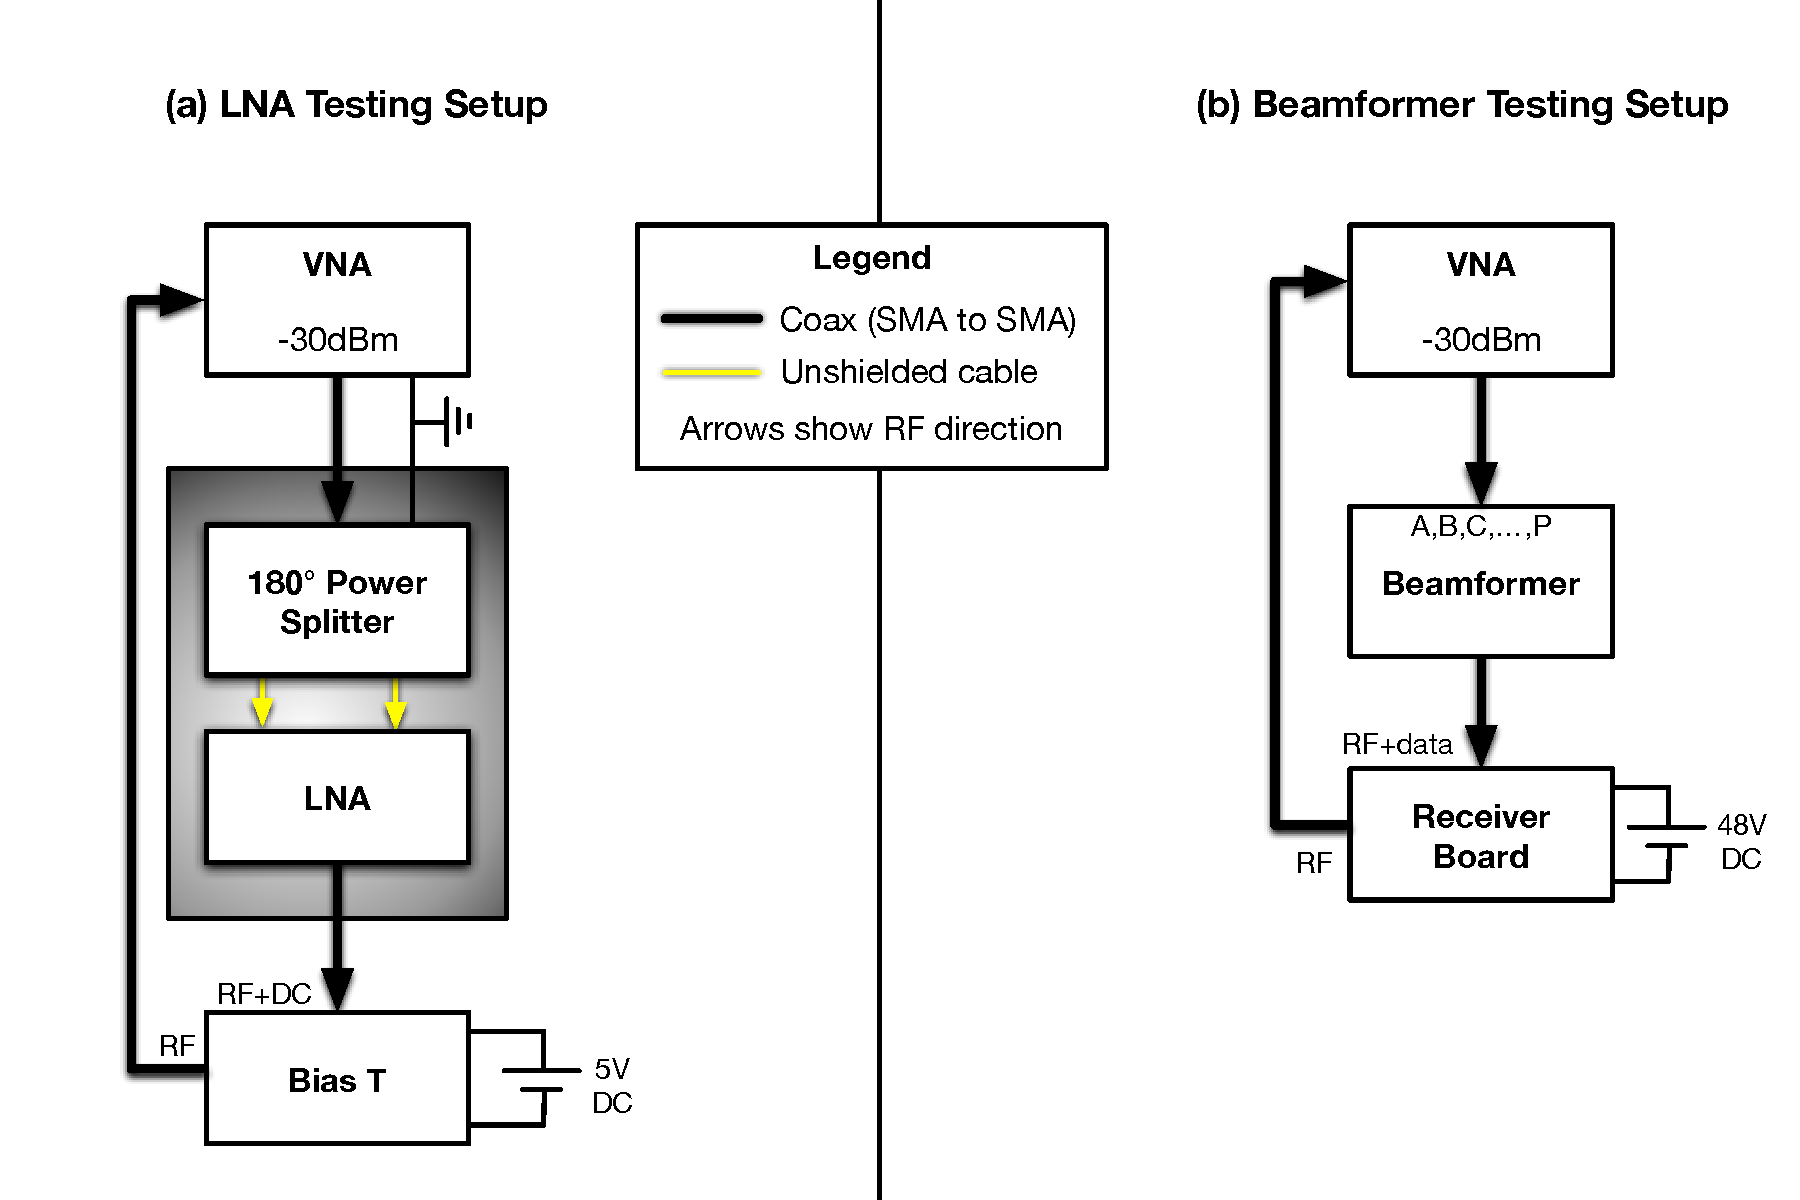
\includegraphics[width=6in]{chap2_beamforming_errors/vna_measurements_diagram.pdf}
\caption[Diagram showing our LNA and beamformer testing setups.]{Diagram showing our LNA and beamformer testing setups (Sec. \ref{sec:lnameasurements}). Note that LNA measurements are conducted above a ground plate to mitigate the effects of exposed antenna leads.}
\label{fig:experimentalsetup}
\end{figure*}

\begin{figure}[b]
\centering
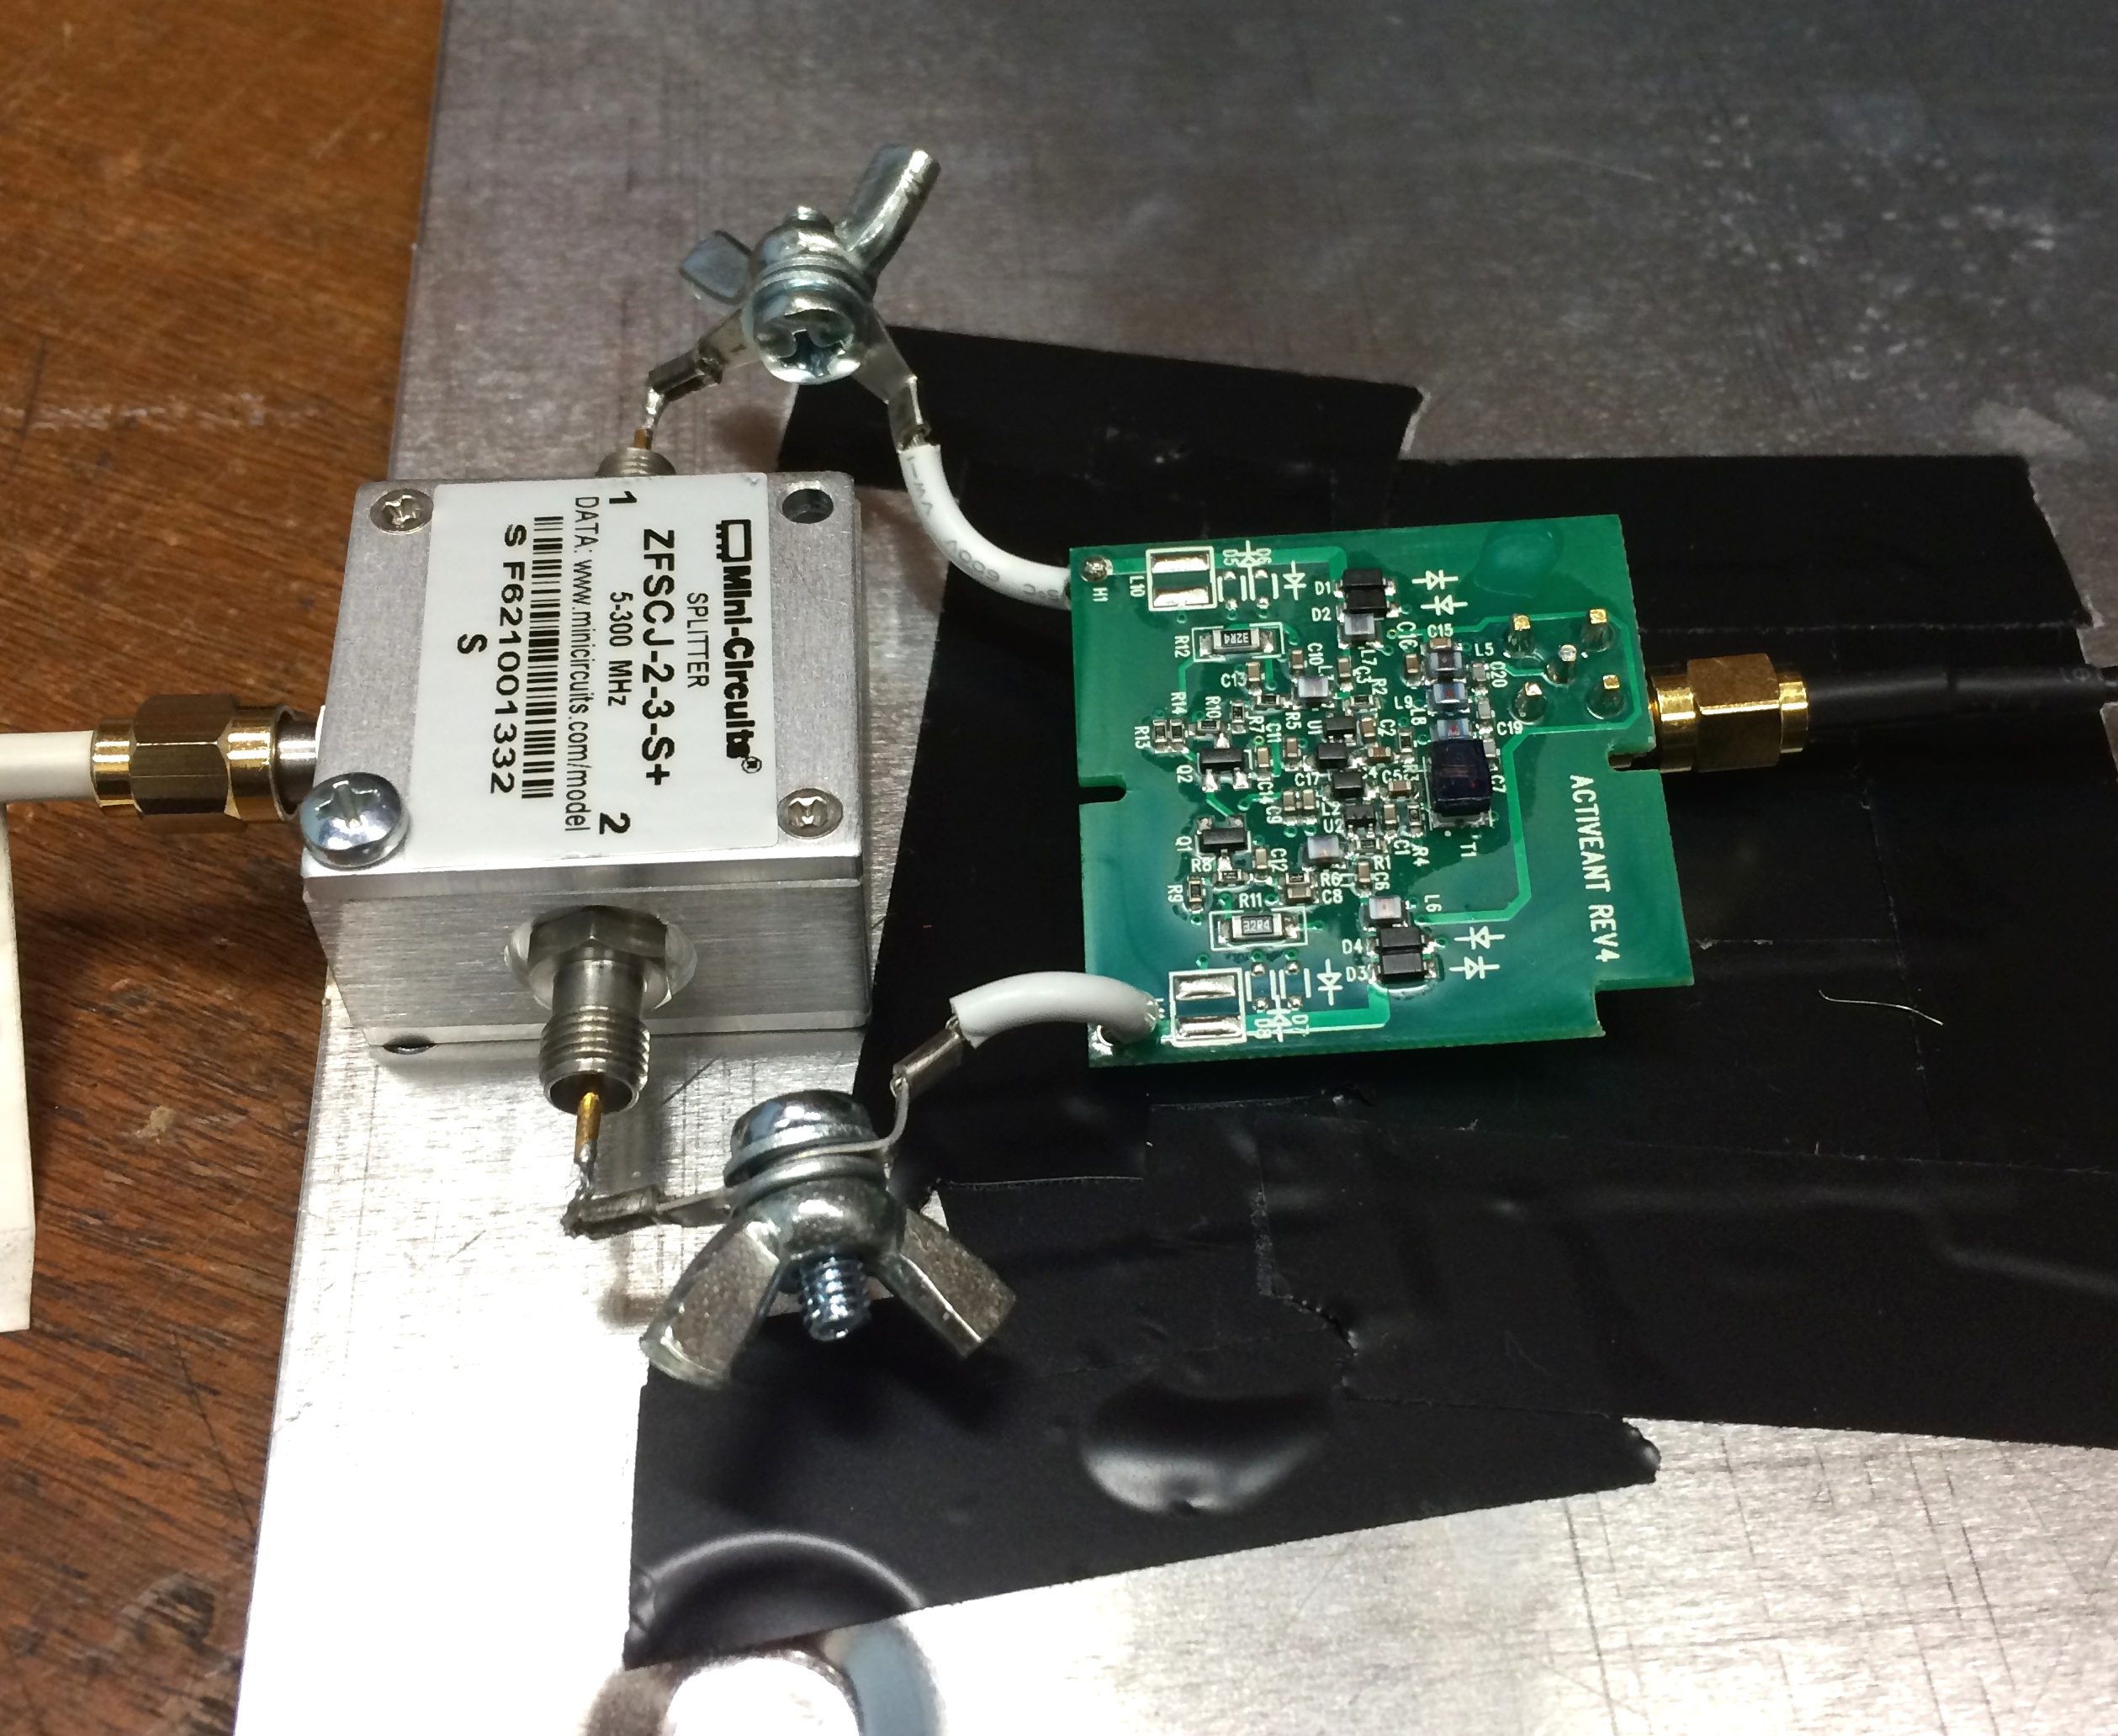
\includegraphics[width=3in]{chap2_beamforming_errors/new_lna_setup.jpg}
\caption[Photograph of the LNA ground plate setup.]{Photograph of the LNA ground plate setup depicted in Figure \ref{fig:experimentalsetup} and described in Sec. \ref{sec:lnameasurements}.}
\label{fig:newlnasetup}
\end{figure}

\begin{figure*}[h]
\centering
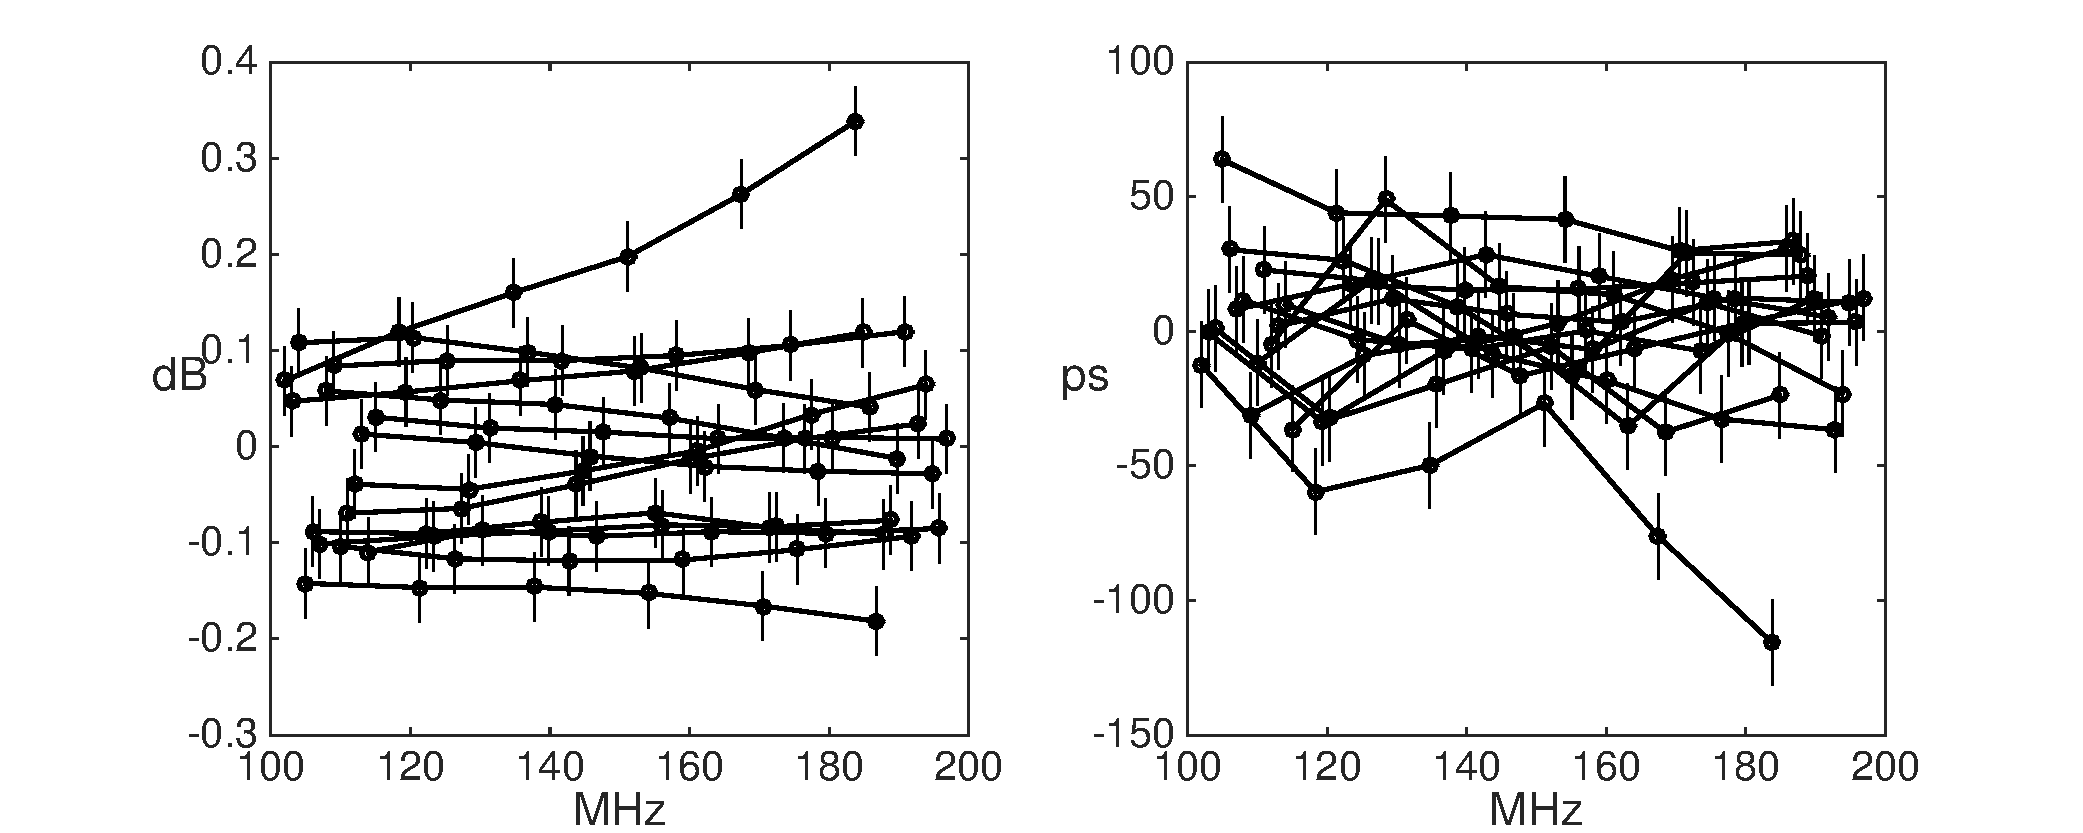
\includegraphics[width=6in]{chap2_beamforming_errors/lnas_gains_delays-eps-converted-to.pdf}
\caption[Gain and group delay measurements on a set of 16 LNAs are shown relative to the mean LNA.]{Gain and group delay measurements on a set of 16 LNAs are shown relative to the mean LNA, as described in Sec. \ref{sec:lnameasurements}. Error bars of $\pm15$\,ps and $\pm0.035$\,dB are the RMS of repeated measuerments. At 150\,MHz, an RMS of 22ps and 0.092dB is observed. Worst cases are observed $2-3\sigma$ away from the mean.}
\label{fig:lnasplot}
\end{figure*}

\begin{figure*}[h]
\centering
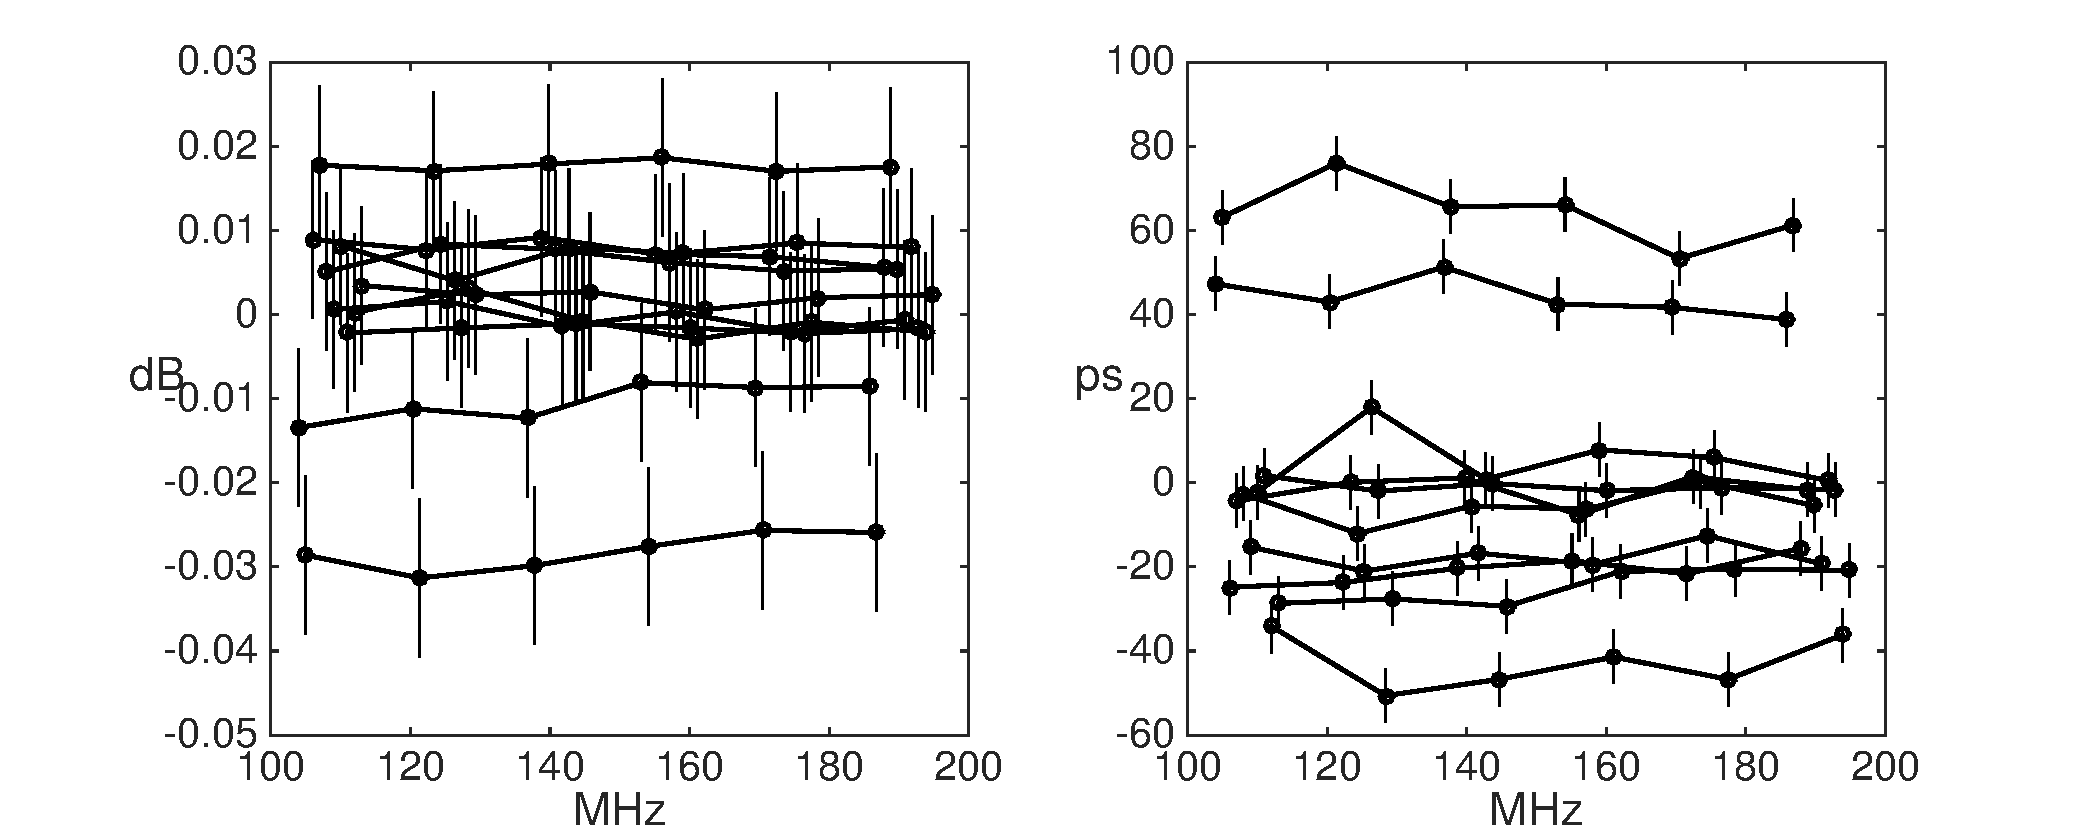
\includegraphics[width=6in]{chap2_beamforming_errors/cables_gains_delays-eps-converted-to.pdf}
\caption[Gain and group delay measurements on a set of 10 dipole cables are shown relative to the mean cable.]{Gain and group delay measurements on a set of 10 dipole cables are shown relative to the mean cable, as described in Sec. \ref{sec:cablemeasurements}. Error bars of $\pm6.2$\,ps and $\pm0.0093$\,dB are the RMS of repeated measurements. At 150\,MHz, an RMS of 34\,ps and 0.013\,dB is observed. Worst cases are observed $2-3\sigma$ away from the mean.}
\label{fig:cablesplot}
\end{figure*}

\begin{figure*}[h]
\centering
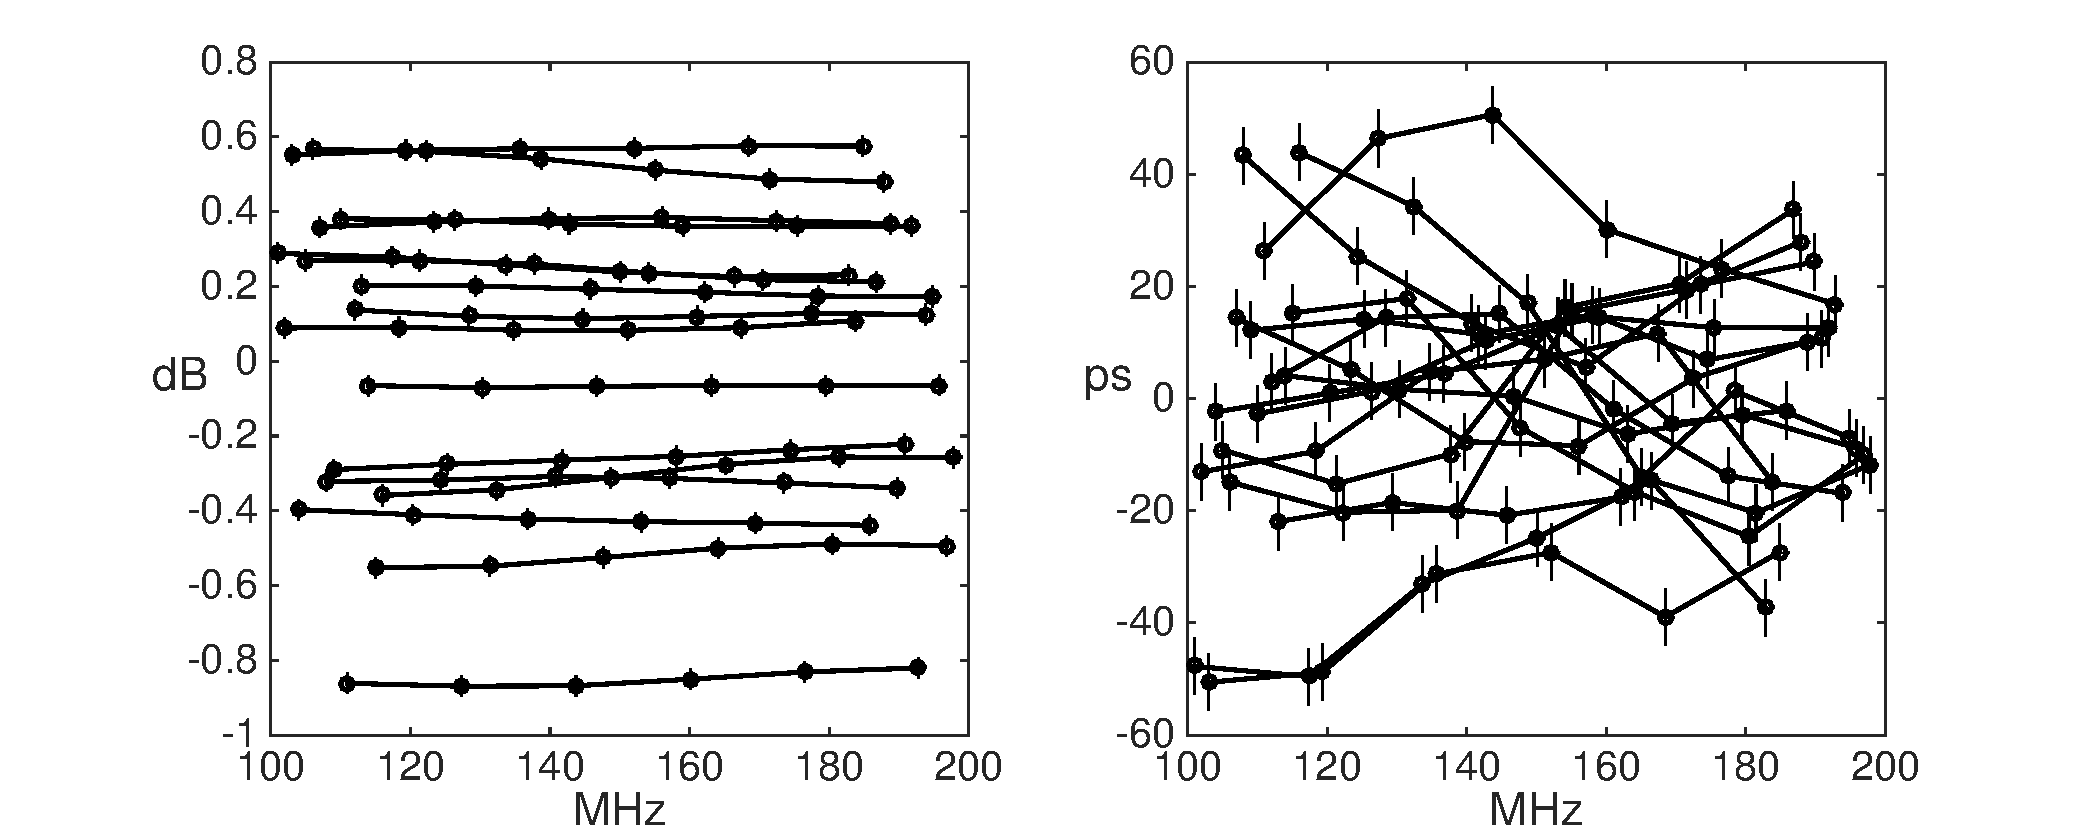
\includegraphics[width=6in]{chap2_beamforming_errors/bf00000_gains_and_delays-eps-converted-to.pdf}
\caption[Gain and group delay measurements on the \textit{shortest} delays of 16 beamformer inputs for one polarization are shown relative to the mean.]{Gain and group delay measurements on the \textit{shortest} delays of 16 beamformer inputs for one polarization are shown relative to the mean, as described in Sec. \ref{sec:bfmeasurements}. Error bars of $\pm4.9$ps and $\pm0.026$\,dB are estimated from repeatability studies. At 150\,MHz, an RMS of 21\,ps and 0.41\,dB is observed. Worst cases are observed $2-3\sigma$ away from the mean.}
\label{fig:bf00000plot}
\end{figure*}

We characterize gain and group delay variation among the cables, LNAs, and beamformer signal paths that comprise an MWA tile through precision vector network analyzer (VNA) measurements of these components. We employ an experimental setup that mitigates the challenges generally faced by such low frequency RF measurements such as reflections at interfaces or due to cable bending, parasitic RF coupling, VNA noise, and saturation of analog components. We discuss uncertainty estimation and perform repeatability checks.

In addition, tilts and misalignments of the deployed MWA tiles contribute to antenna-to-antenna beam variation and concomitant beam mismodeling. We characterize these effects using the known MWA tile positions and elevations.

\subsection{Gain and Group Delay Experiments}

Gain and group delay measurements are conducted on LNAs, dipole cables, and beamformer paths using the setups described in more detail in the sections below. In all cases, we perform measurements over the band $100-200$\,MHz, then retain the group delay and gain RMS at 150\,MHz for our beamforming error budget; the RMS is observed to be relatively frequency-independent over this band. Note that the physical gains and phases show some frequency dependence across this band, but \textit{only relative differences between the sixteen dipole pathways distort the beam pattern}. The mean gain and group delay through the 16 signal paths are absorbed into each tile's calibration amplitude and phase. For the same reason, gains and group delays of the VNA and measurement cables are irrelevant.

We use an Anritsu MS2024A vector network analyzer set to low probe power (-30\,dBm) and 30 trace averaging. The VNA is optimized for wide band (GHz) measurements, and we mitigate small-scale (sub MHz) systematics through binning to 16\,MHz. In each of these windows, we average the gains measured at 0.36\,MHz resolution, and compute the mean group delay by fitting a ramp to the measured phases. We perform repeated measurements on each component after disconnecting and reconnecting the entire measurement setup in order to estimate uncertainties due to slight bending of probe cables or imperfect cable connections.

\subsubsection{LNA Measurements}
\label{sec:lnameasurements}

Precision LNA measurements are particularly challenging in a laboratory setting given their exposed leads which, in a deployment environment, are fed balanced input by two dipole arms. Figure \ref{fig:experimentalsetup}(a) shows a diagram of our solution. We use a 180$^\circ$ two-way power splitter (Mini-Circuits ZFSCJ-2-3-S+) to split the VNA probe signal into two balanced inputs to the LNA, both mounted above an aluminum plate to mitigate RF coupling (Figure \ref{fig:newlnasetup}). The aluminum plate is grounded  to the splitter case, and then to the VNA probe cable shield. We fabricated angle connectors to secure the LNA leads to the center conductors of the power splitter outputs with as little exposed wire as possible. The LNA is powered through a Bias-T (Mini-Circuits ZFBT-4R2G-FT+) with a 5\,VDC power supply. 

We use this testing setup to characterize 16 single-polarization LNAs. Due to their different cable lead lengths, the X and Y boards have systematically different group delays which we correct for the subsequent analysis. As bending of these leads contributes to group delay variation among different LNAs, the LNA design was subsequently modified to fit both polarizations  on the same circuit board and eliminate the excess lead cable. To approximate the level of group delay variation in these dual-polarization LNAs, we estimate the group delay variance contributed by the cable leads as equal to the measurement uncertainty (assumed dominated by cable lead bending), and subtract it from the total observed group delay variance for the single-polarization LNAs. Figure \ref{fig:lnasplot} shows our measured gains and group delays with measurement uncertainties of $\pm0.03$\,dB and $\pm15$\,ps through repeated measurements on the same set of LNAs. Measurements on different LNAs are slightly offset in frequency for ease of comparison. We observe significant (relative to measurement uncertainty) gain and group delay RMS at 150\,MHz of 21\,ps and 0.09\,dB, with worst cases $2-3\sigma$ away from the mean. Subtracting (in quadrature) the 15\,ps measurement uncertainty due to cable bending from the total delay RMS yields the intrinsic LNA delay RMS of 15\,ps.

\subsubsection{Cable Measurements}
\label{sec:cablemeasurements}

Figure \ref{fig:cablesplot} shows our dipole cable gain and group delay measurements relative to an average cable, with RMS measurement errors of $\pm0.0093$\,dB and $\pm6.2$\,ps. At 150\,MHz, we observe a significant (relative to the measurement error) group delay scatter of 34\,ps RMS and an insignificant gain scatter of 0.013dB RMS. Outliers are seen $2-3\sigma$ away from the mean. The dipoles cables are specified to be phase matched to $\pm1-3^\circ$ over $100-200$\,MHz. This translates into a group delay RMS of $\pm19-55$\,ps, and is consistent with our measurements.

\subsubsection{Beamformer Measurements}
\label{sec:bfmeasurements}

Gains and group delays of a set of 16 beamformer inputs for one polarization were measured in a testing setup depicted in Figure \ref{fig:experimentalsetup}(b). To avoid bending of the VNA probe cable when moving it across the 16 beamformer inputs, a dipole cable was used to connect the VNA probe cable to the desired beamformer input. Figure \ref{fig:bf00000plot} shows our measured gains and group delays for the shortest delays on these 16 beamformer inputs with measurement uncertainties of 4.9\,ps and 0.026\,dB. We observe an RMS of 21\,ps and 0.4\,dB at 150\,MHz, with worst cases $2-3\sigma$ from the mean. The longest delays through these beamformer inputs correspond to all delay lines (``bits'') engaged, yielding $\sim13.5$\,ns of delay. We also probe the maximum delays through these beamformer inputs and find RMS's of 54\,ps and 0.43\,dB at 150\,MHz.

\subsection{Tile Tilts and Rotation}

\begin{figure*}[t]
\centering
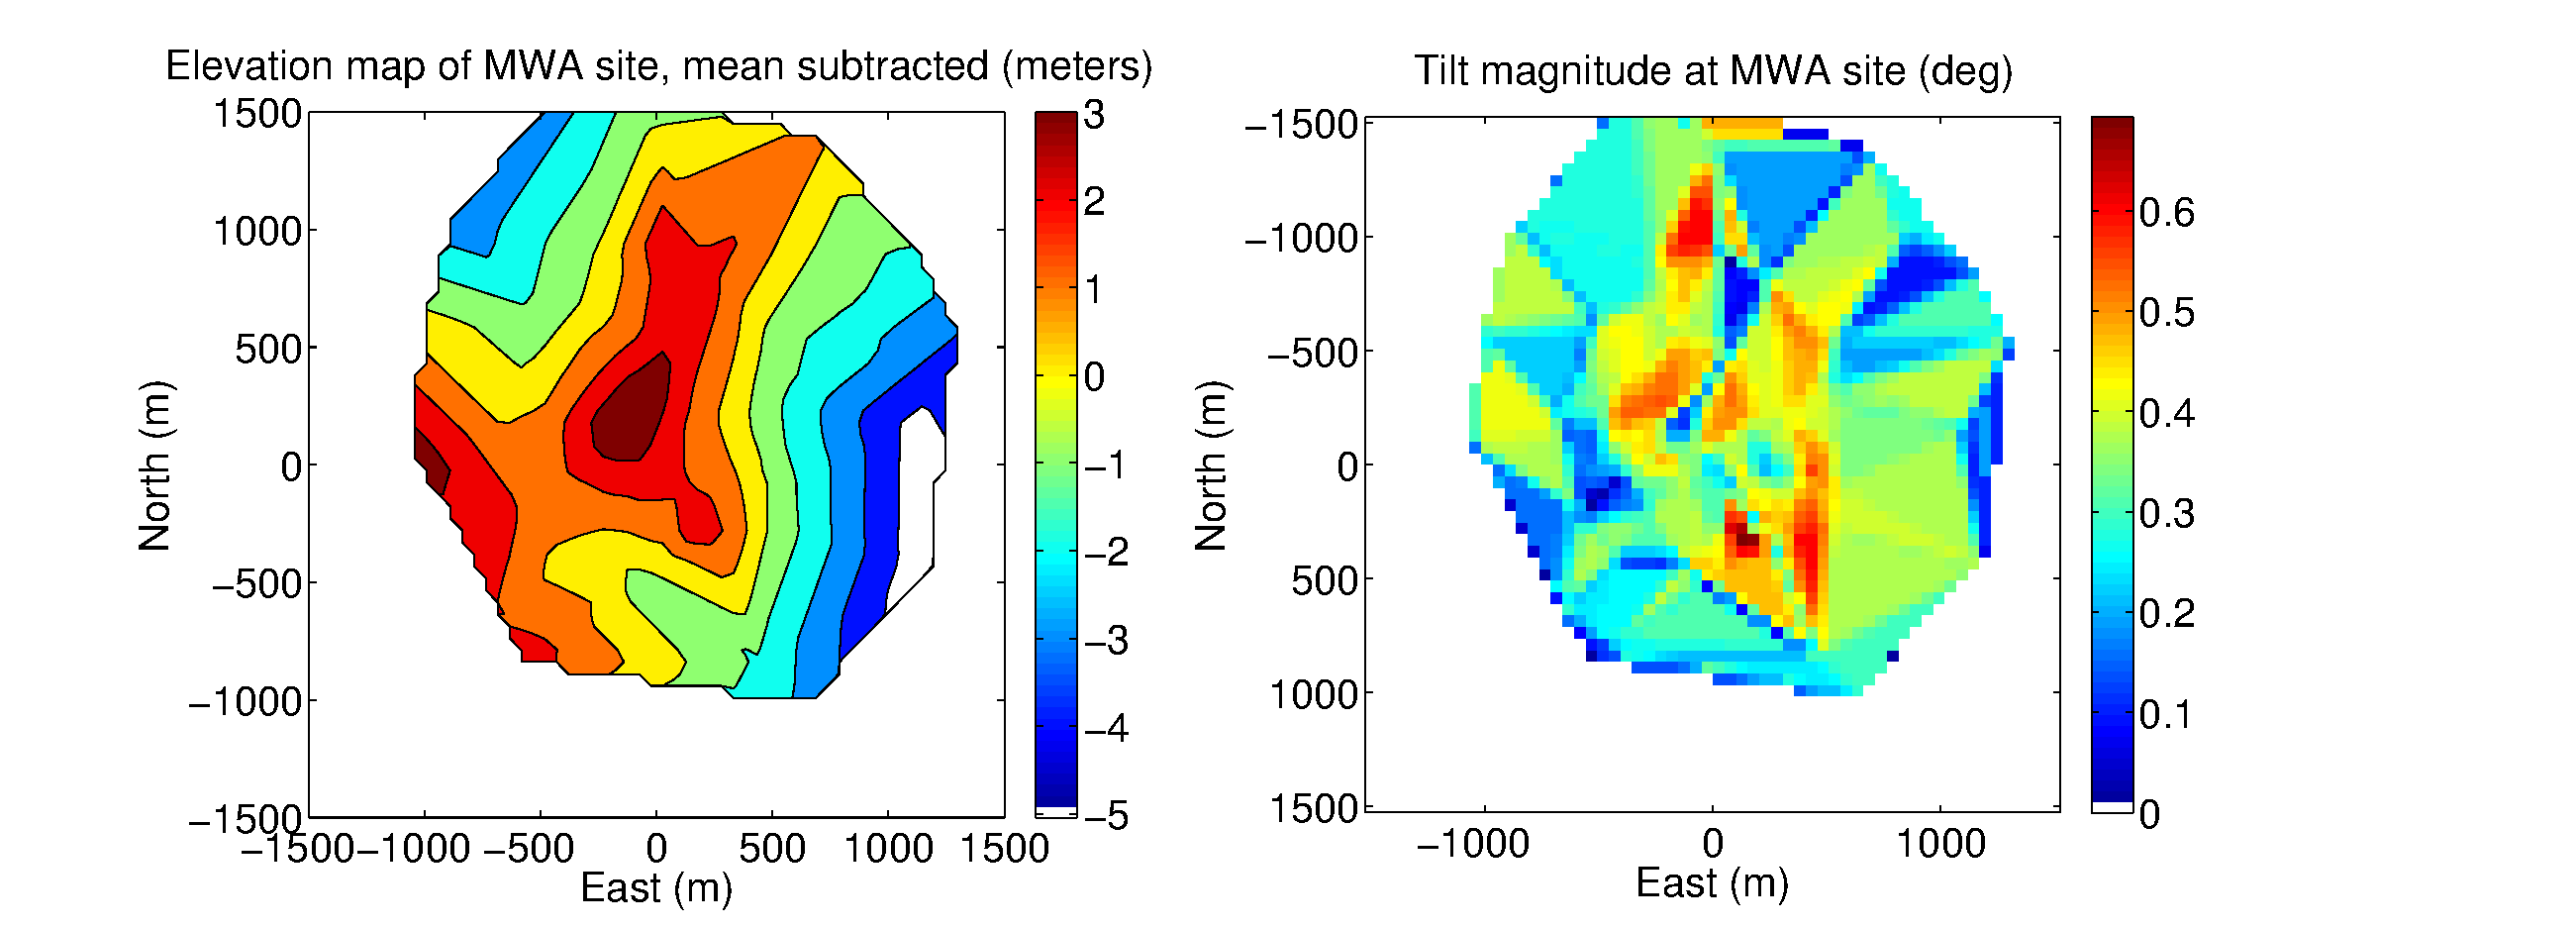
\includegraphics[width=7in]{chap2_beamforming_errors/mwa_tilt_map-eps-converted-to.pdf}
\caption[Map of the tilt magnitude of the MWA site.]{Map of the tilt magnitude of the MWA site computed by gridding the 3D tile positions and taking the gradient. Triangular features are artifacts from sparse grid coverage by the antenna positions, nonetheless their magnitudes are likely reasonable approximations, perhaps even underestimates of the land tilts given that small scale topographic structure is unconstrained.}
\label{fig:mwatiletiltmap}
\end{figure*}

As the MWA was constructed around the apex of a slight hill to avoid flooding, a planar fit to the tile positions is quite poor. In principle tile tilts and rotations could be measured and incorporated into data reduction, however this has not yet been done. In this paper, we conservatively incorporate them into our budget of antenna-to-antenna variation. We estimate tile tilts by gridding the differential GPS mapped tile positions, then compute the magnitude of the gradient. Using a 60\,m grid spacing we find the RMS of the tilt (away from zenith) magnitude to be $0.27^\circ$, with some tiles having tilts up to $0.4^\circ$ (Figure \ref{fig:mwatiletiltmap}). These numbers are of order the precision of the differential GPS measurements used to determine the tile corners, so for simplicity we assume an RMS of $\sim0.3^\circ$ for EW tilt, NS tilt, and rotation in subsequent simulations. 

\subsection{Budget of Beamforming Errors}
\label{sec:budget}

We compile the measurements presented in this section into a budget of beamforming errors in Table \ref{table:systematictable}. Additionally we include the estimated dipole position precision of $0-17$\,ps estimated in Sec. \ref{sec:groundscreen} as it is comparable with the other sources of group delay scatter. Summing these group delay scatters in quadrature gives a total RMS of 46\,ps (68 \,ps) using the shortest (longest) beamformer delays. In contrast, the gain scatter is dominated by variation over the beamformer inputs of 0.4\,dB for both delay settings. Lastly, overall tilts and rotations of the tile with $0.3^\circ$ RMS are included separately.

% table showing beamforming errors budget
 \begin{table}[h]
 \centering
 \caption{ \label{table:systematictable}Beamforming error budget at 150\,MHz.}
 \begin{tabular}{llllllll}
 \hline\hline
 Systematic Name & RMS \\
 \hline\hline
Cable group delay & 34\,ps \\
LNA delay & 15\,ps  \\
Beamformer delay (shortest delay) & 21\,ps   \\
Beamformer delay (longest delay) & 54\,ps   \\
Dipole position & $0-17$ps & \\
\hline
Cable gain & 0.013\,dB\\
LNA gain & 0.09\,dB \\
Beamformer gain (shortest delay) & 0.41\,dB \\
Beamformer gain (longest delay) & 0.43\,dB \\
\hline
Tile tilt/rotation & 0.27$^\circ$ \\
     \hline\\
 \end{tabular}
 \end{table}

% simulations
\section{Simulating Beams with Beamforming Errors}
\label{sec:simulations}

\begin{figure*}[h]
\centering
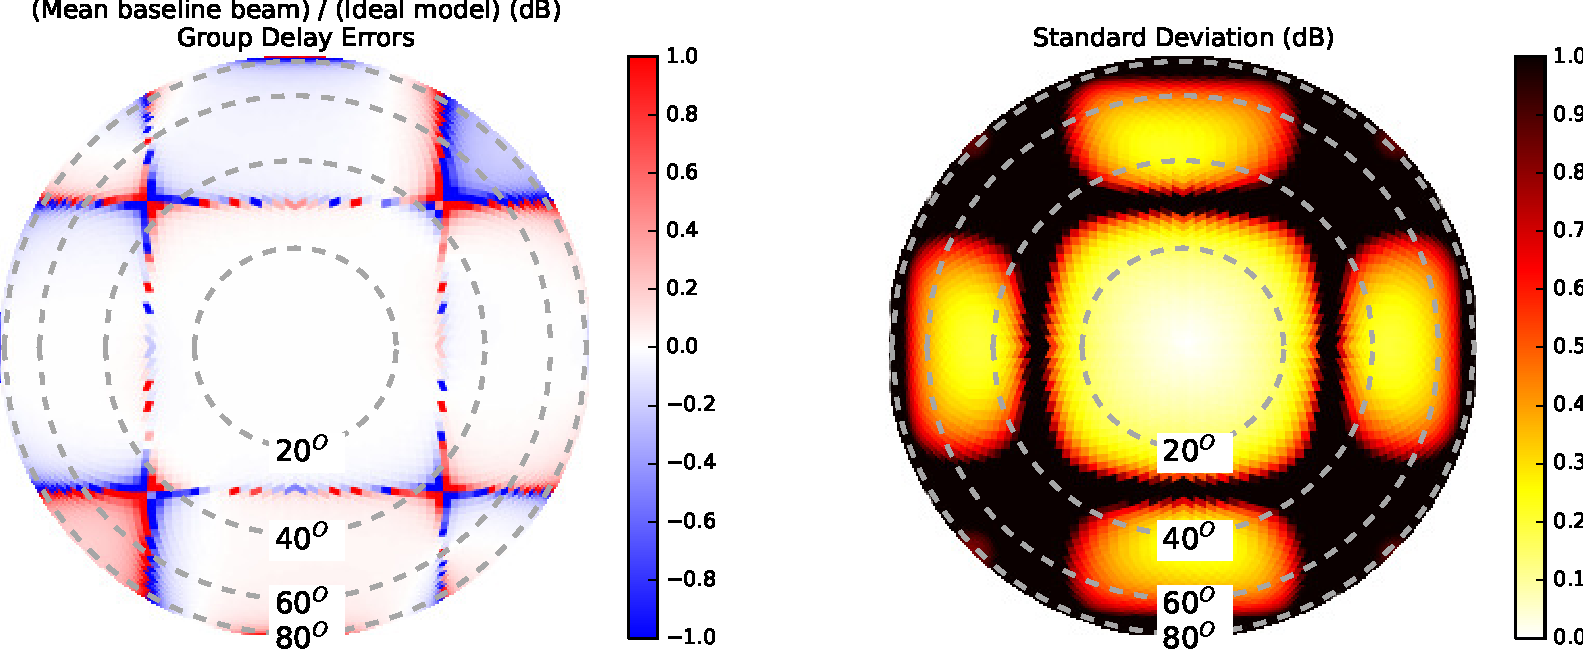
\includegraphics[width=5in]{chap2_beamforming_errors/groupdelays50ps_baselinemean_and_std_power_beamzenith-eps-converted-to.pdf}
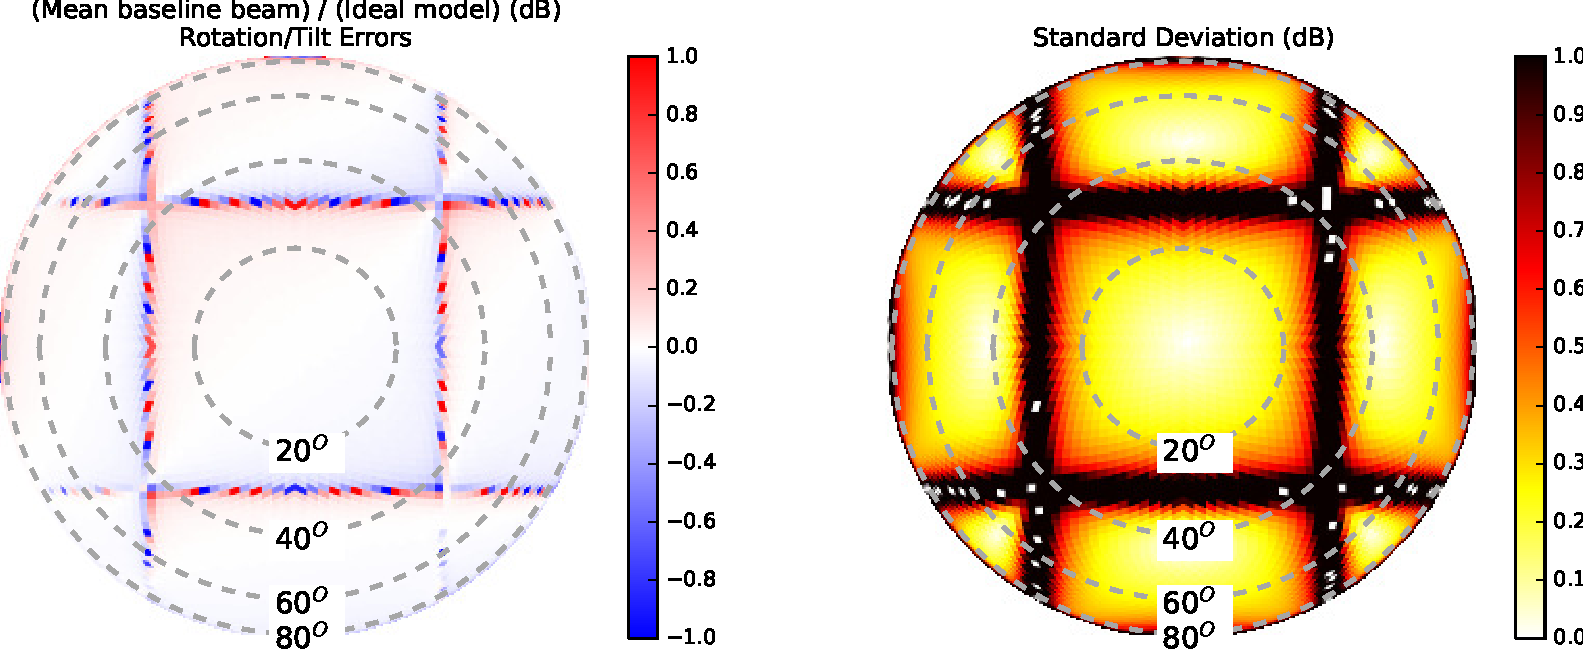
\includegraphics[width=5in]{chap2_beamforming_errors/thetaall0_3deg_baselinemean_and_std_power_beamzenith-eps-converted-to.pdf}
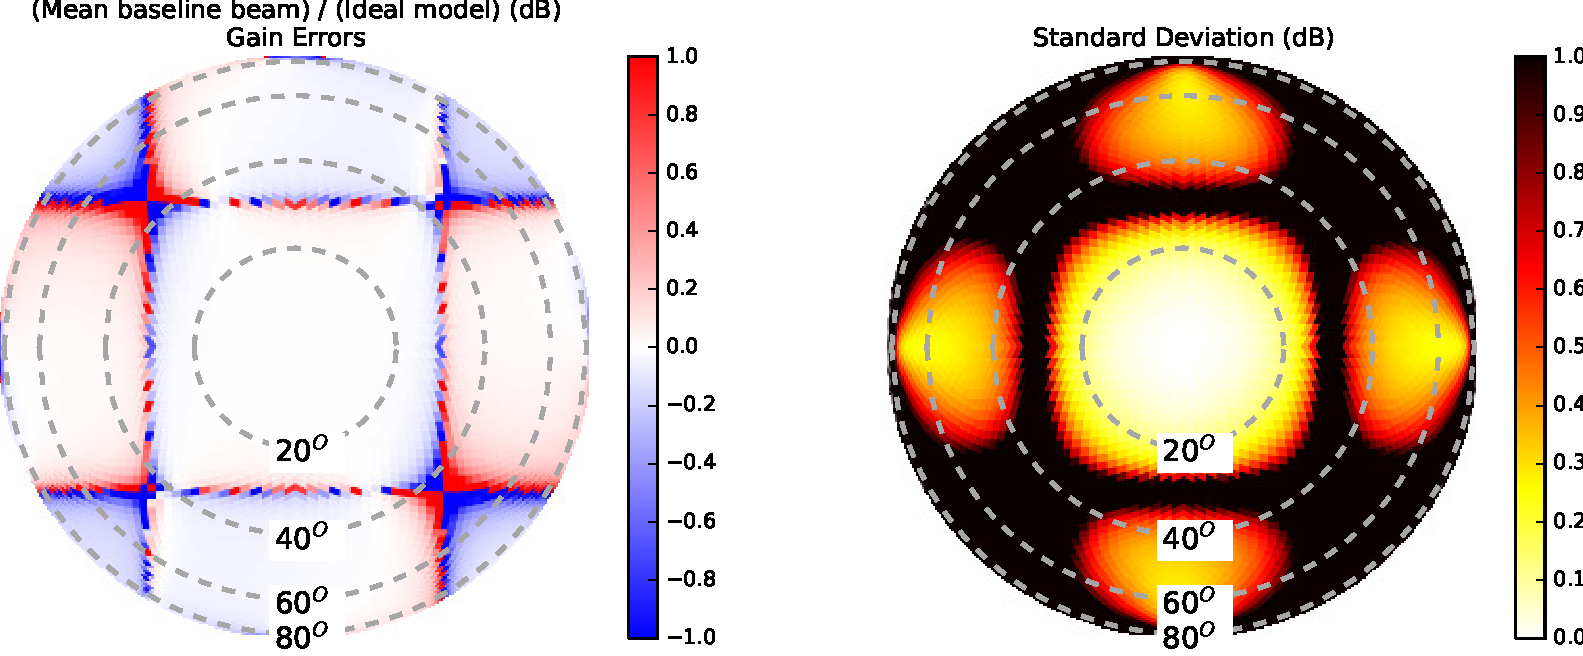
\includegraphics[width=5in]{chap2_beamforming_errors/gains0_5dB_baselinemean_and_std_power_beamzenith-eps-converted-to.pdf}
\caption[Baseline-averaged beam (left) and standard deviation (right) of simulated beams relative to the ideal model.]{Baseline-averaged beam (left) and standard deviation (right) of simulated beams relative to the ideal model: $\sigma_\text{delay}=50$\,ps group delays (top), $\sigma_\text{tilt,rot}=0.3^\circ$ (middle), and $\sigma_\text{gain}=0.5$\,dB (bottom). Even though the individual beams exhibit fluctuations at the $0.2-0.5$\,dB level near the edge of the mean lobe and in the sidelobes, the effects on the baseline-averaged beam are at the sub-percent level except within several degrees of the sidelobes. This is due to partial cancellation of the complex beam errors when combining the complex pair-product beams of different visibilities, here calculated assuming natural weighting. The color scale in the right panel is saturated at 1\,dB.}
\label{fig:simdelaysthetagains}
\end{figure*}

\begin{figure*}[t]
\centering
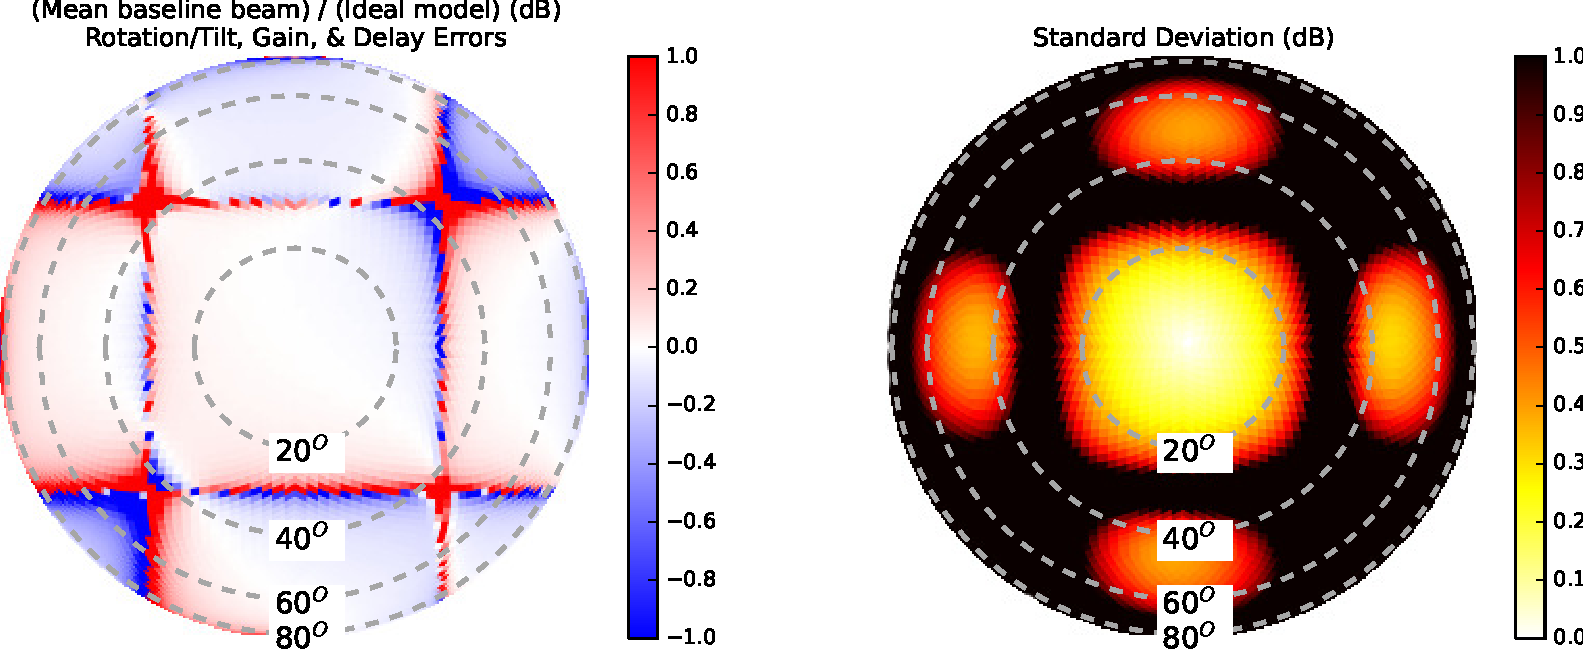
\includegraphics[width=6in]{chap2_beamforming_errors/groupdelays50psgains0_5dBthetaall0_3deg_baselinemean_and_std_power_beamzenith-eps-converted-to.pdf}
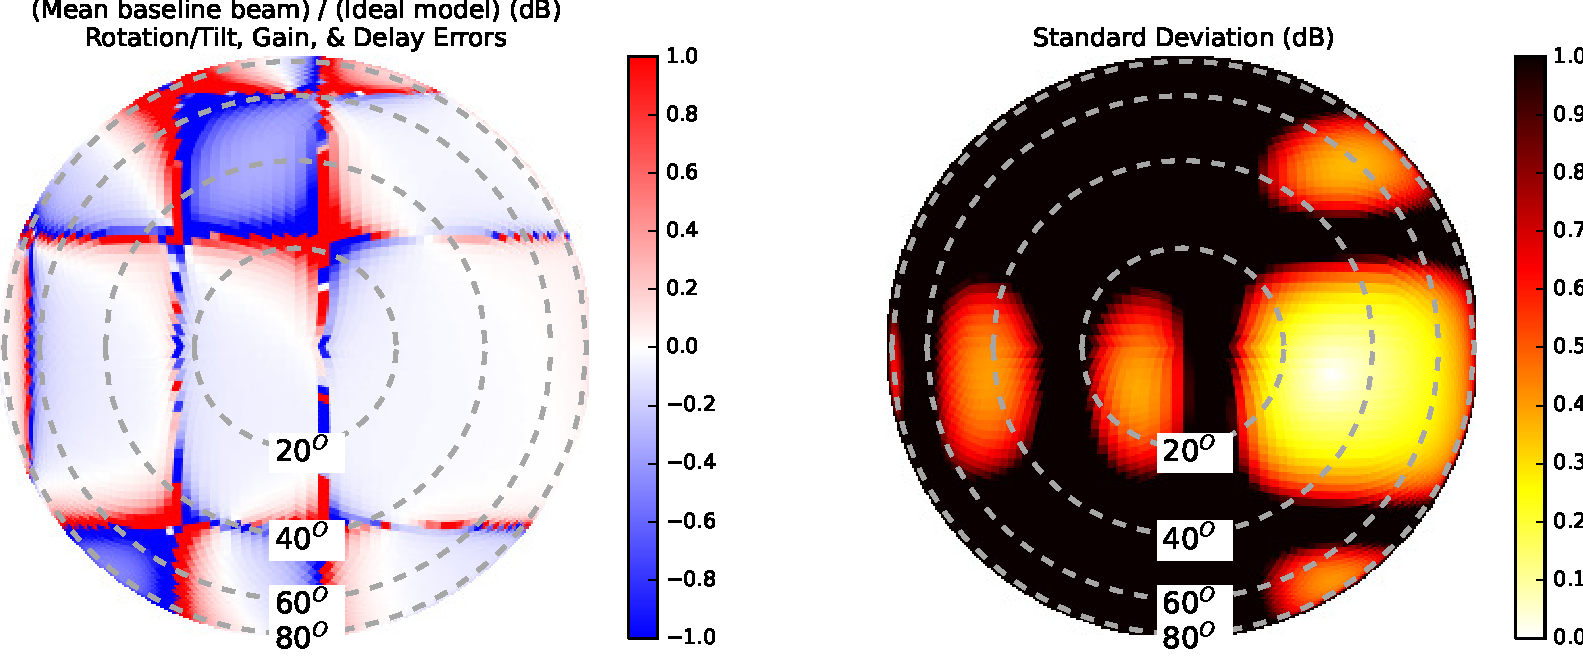
\includegraphics[width=6in]{chap2_beamforming_errors/groupdelays50psgains0_5dBthetaall0_3deg_baselinemean_and_std_power_beamoffzenith-eps-converted-to.pdf}
\caption[Baseline-averaged beam (left) and standard deviation (right) of simulated beams using the full beamforming error budget.]{Baseline-averaged beam (left) and standard deviation (right) of simulated beams using the full beamforming error budget ($\sigma_\text{delay}=50$\,ps group delays, $\sigma_\text{tilt,rot}=0.3^\circ$, and $\sigma_\text{gain}=0.5$\,dB) for a zenith pointing (top) and the off-zenith pointing (bottom). }
\label{fig:simall}
\end{figure*}

\begin{figure*}[h]
\centering
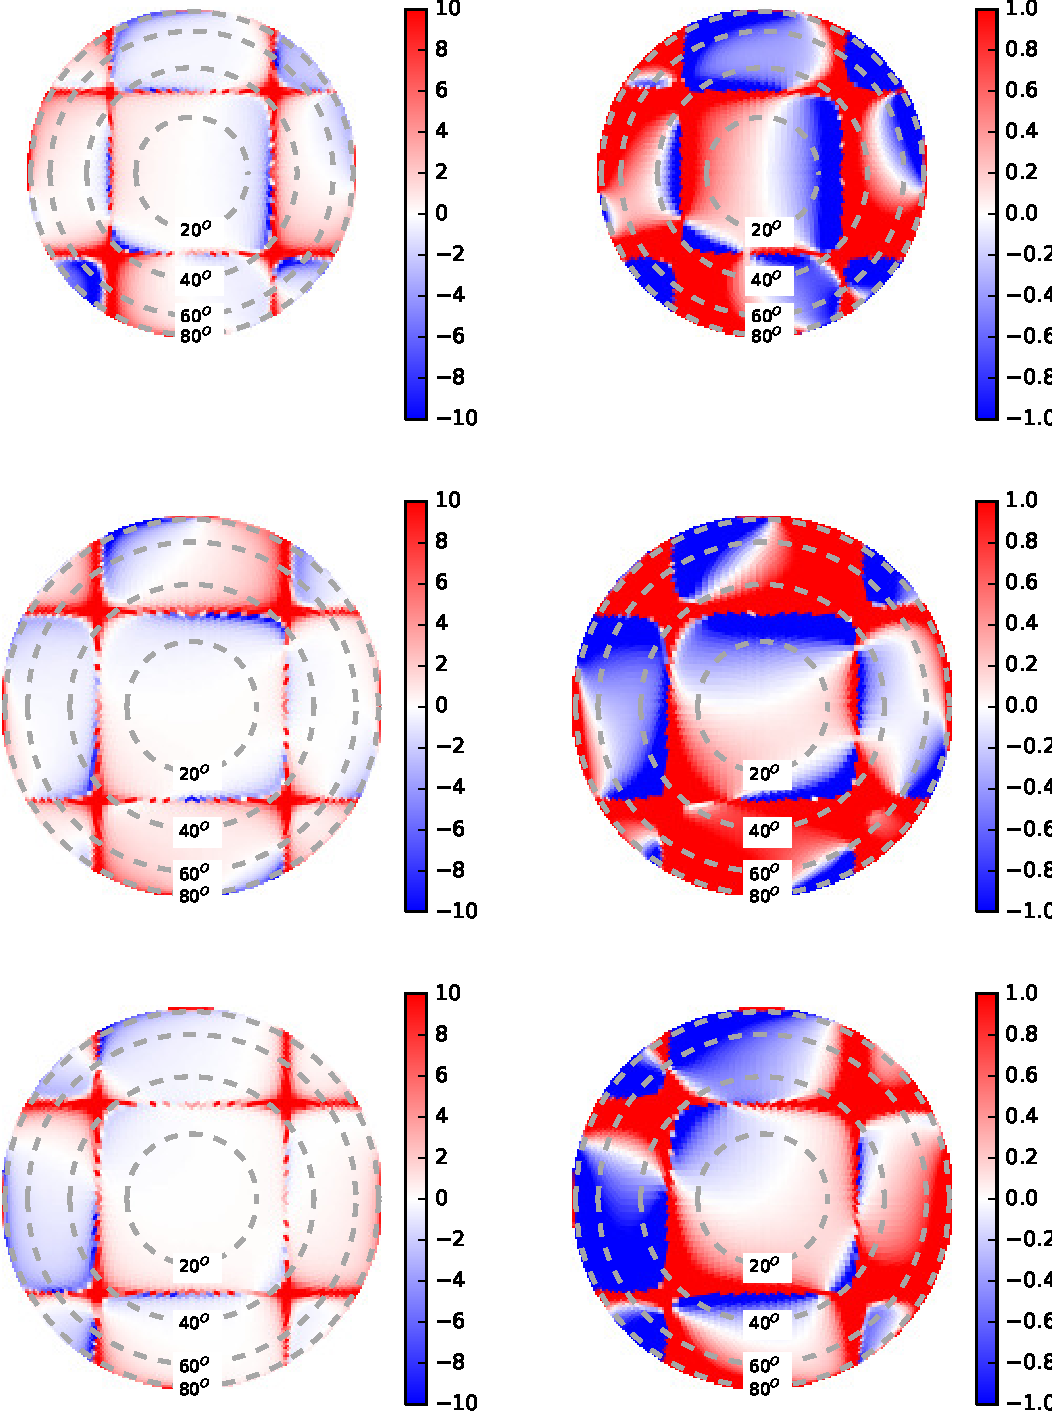
\includegraphics[width=5in]{chap2_beamforming_errors/groupdelays50psgains0_5dBthetaall0_3deg_simbeams-eps-converted-to.pdf}
\caption[Each row shows a realization of a simulated beam relative to the ideal beam.]{Each row shows a realization of a simulated beam relative to the ideal beam (in dB) on a compressed color scale (left) and on an expanded color scale (right). This simulation used the full beamforming error budget of $\sigma_\text{delay}=50$\,ps, $\sigma_\text{gain}=0.5$\,dB, $\sigma_\text{tilt,rot}=0.3^\circ$. Here we see up and down fluctuations in the sidelobes and near the nulls (right) at the $\pm0.5$\,dB level seen in Figure \ref{fig:simall}, in addition to a positive bias within several degrees of the nulls (left). }
\label{fig:simallsamples}
\end{figure*}

\begin{figure*}[h]
\centering
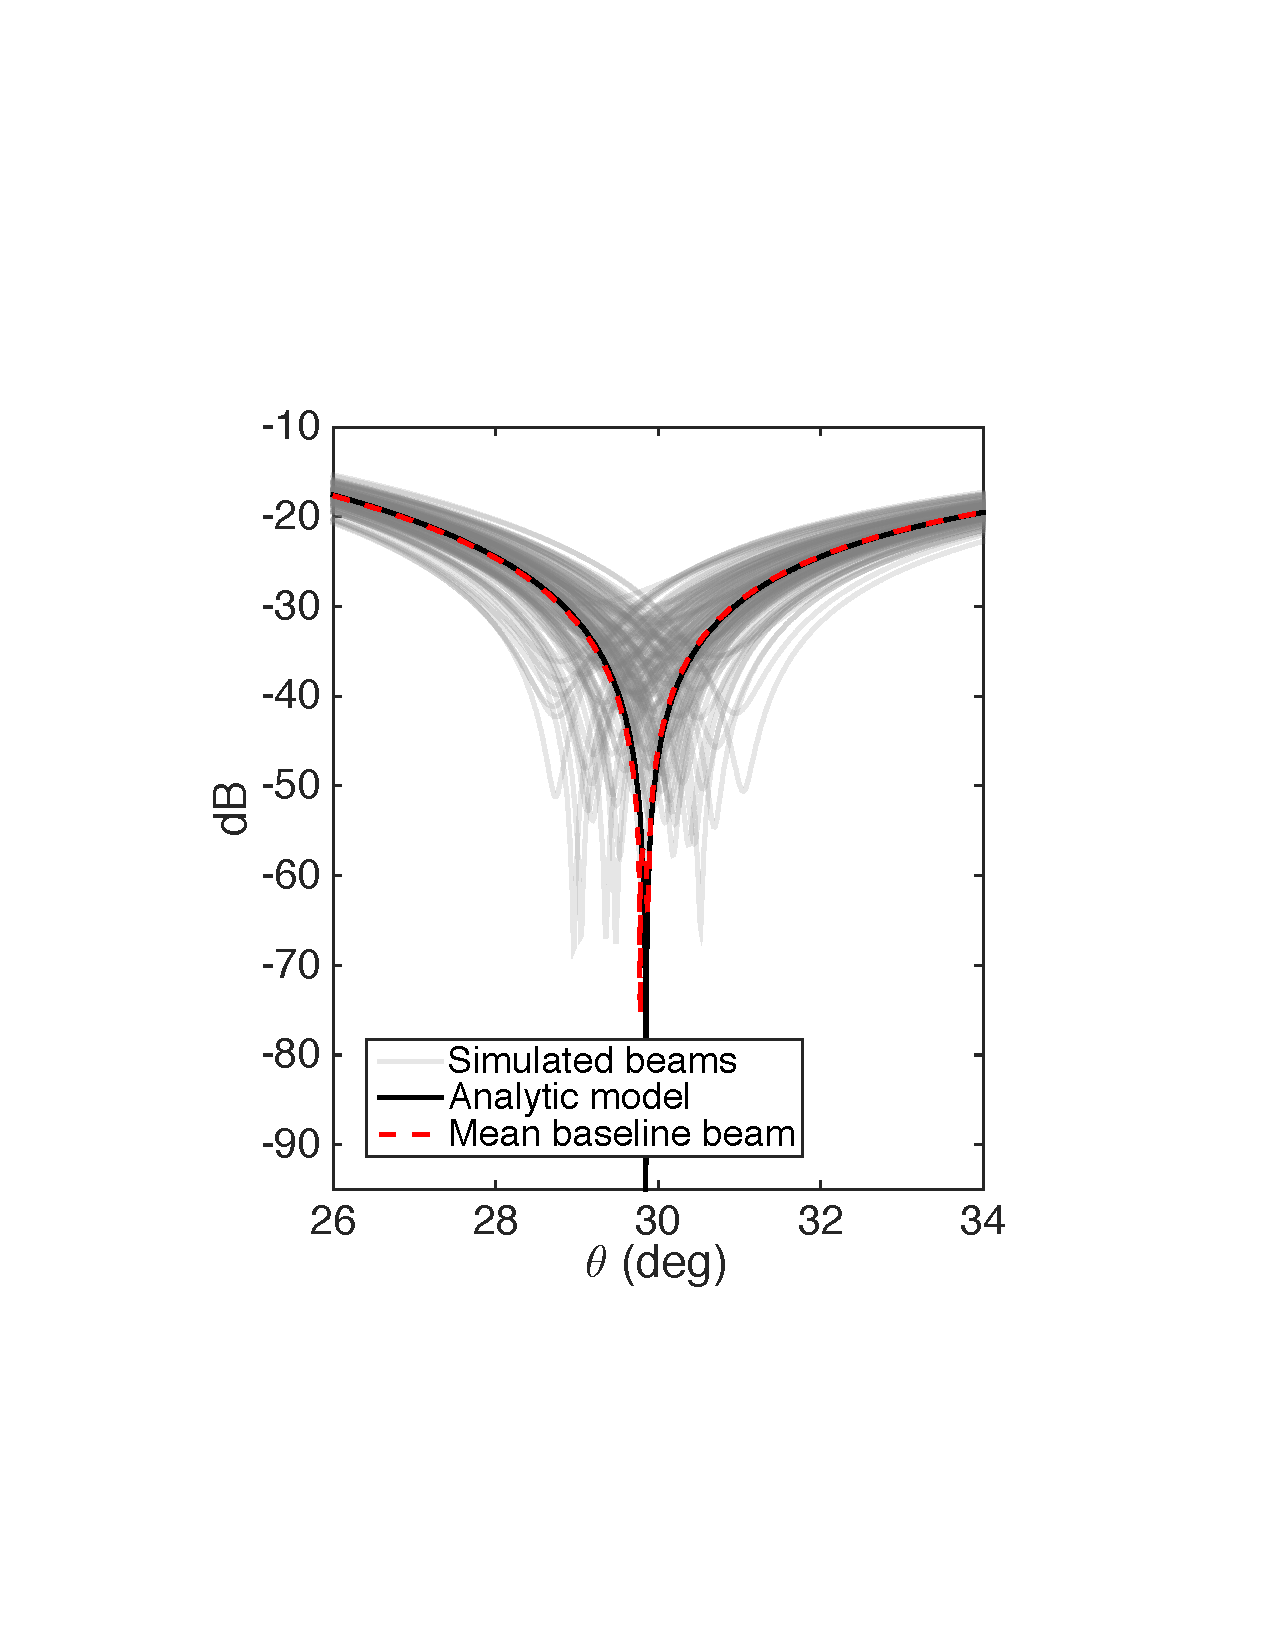
\includegraphics[width=2.9in]{chap2_beamforming_errors/test_beam_averaging_zoom1.pdf}
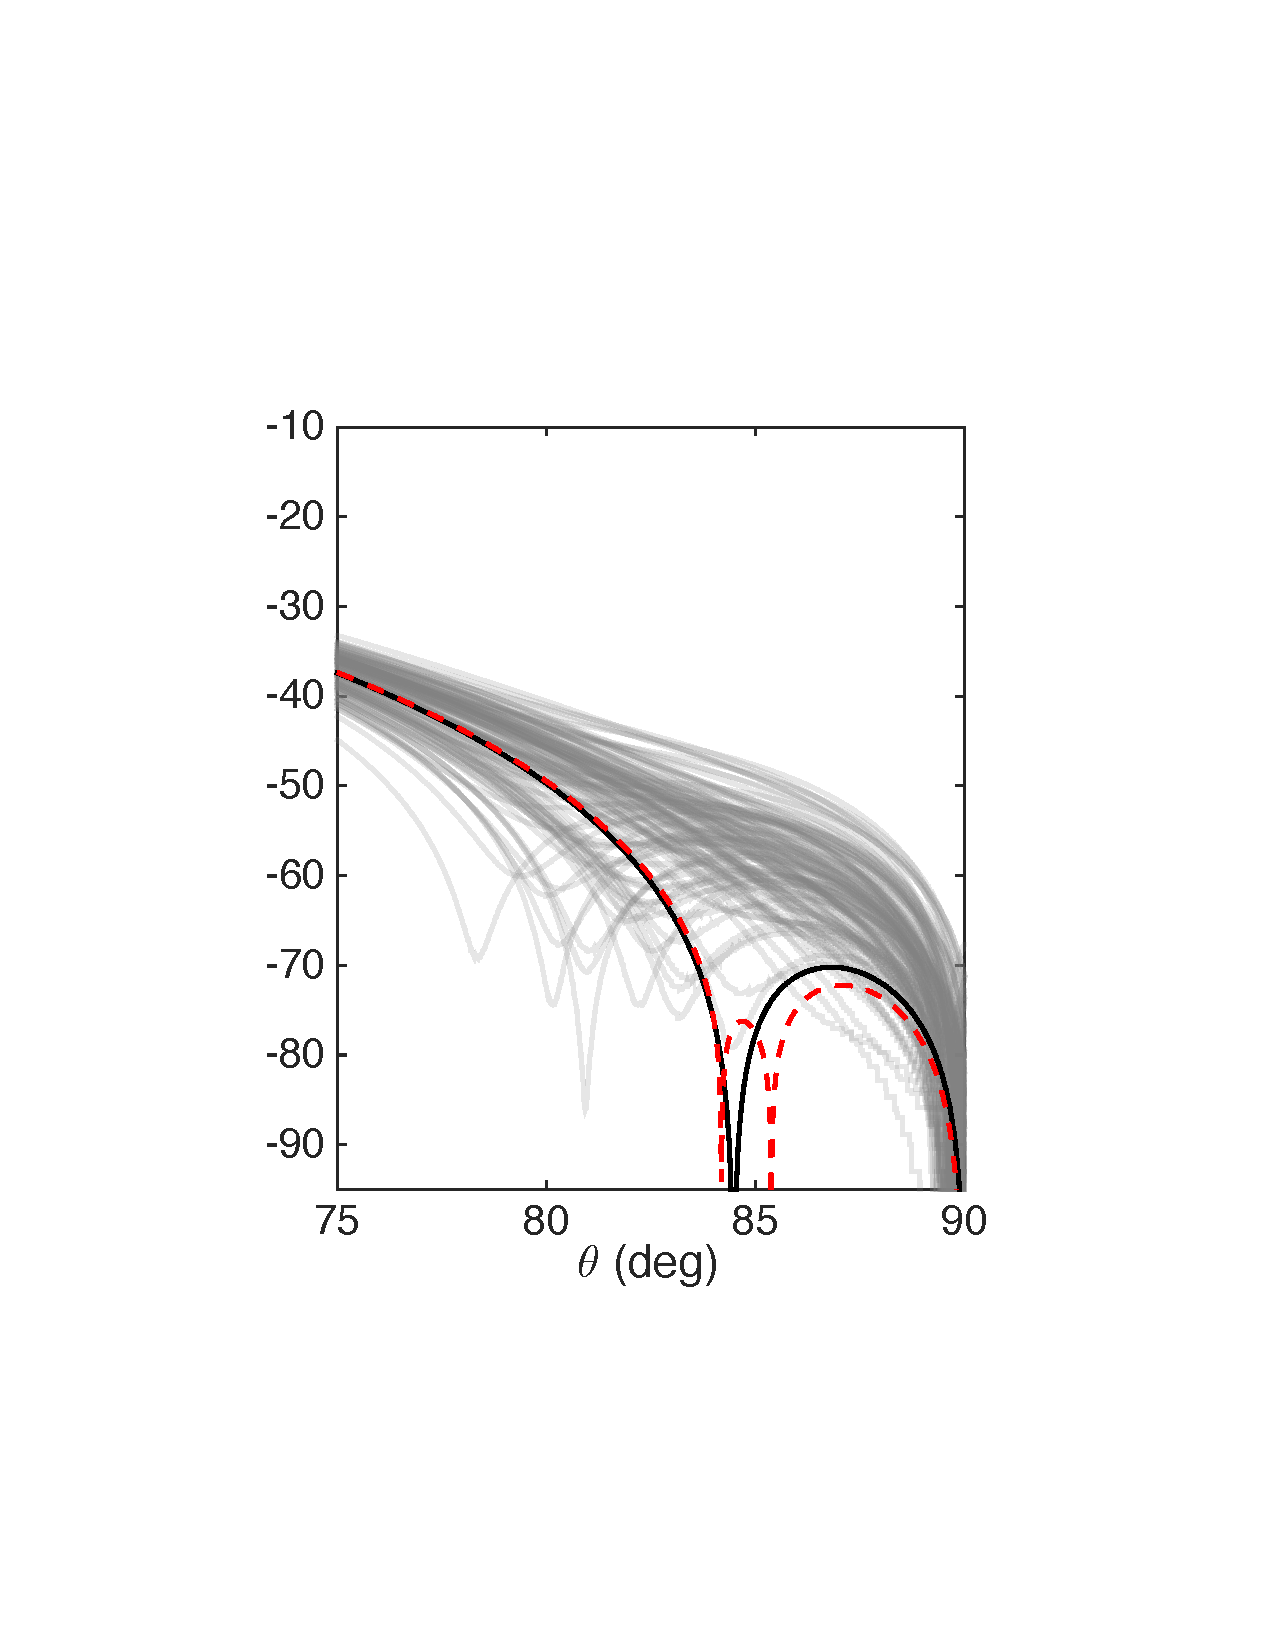
\includegraphics[width=2.7in]{chap2_beamforming_errors/test_beam_averaging_zoom2.pdf}
\caption[Zoom in around the first null and near the horizon along a NS slice through the beam in full beamforming errors simulations.]{We zoom in around the first null and near the horizon along a NS slice through the beam after running simulations with our full beamforming errors budget with $0.01^\circ$ resolution. The nulls in all 128 beams with beamforming errors ($|b_i|^2$) (gray) are ``filled in'' by the errors, however the baseline-averaged beam (Eqn. \ref{eqn:meanbaselinebeam}) (red dashed) remains very close to the ideal power beam ($|b|^2$) (black) for the reasons discussed in Sec. \ref{sec:simulations}. This demonstrates that beamforming fluctuations of different antennas tend to average out in imaging. Still, the antenna-to-antenna variation will limit deconvolution accuracy.}
\label{fig:sidelobeaveraging}
\end{figure*}


We study the separate and cumulative effects of beamforming errors on beam patterns through simulations using the budget presented in Sec. \ref{sec:budget}, assuming that the dipole gain and delay errors and the tile tilts and rotations are randomly scattered around zero. We incorporate these errors into a simple analytic beam model and compute statistics on the set of slightly corrupted beams. Extensive numerical modeling \citep{sutinjo15} shows slight corrections relative to the analytic model towards the edge of the main lobe and in the sidelobes, especially at higher frequencies towards 200\,MHz, but is susceptible to beamforming errors in largely the same way as the analytic beam. 

The analytic electric field beam, $b(\theta,\phi,\lambda)$, models the tile as a $4\times4$ grid of EW-oriented Hertzian dipoles above a perfect, infinite ground plane, with no mutual coupling,
\begin{eqnarray}
\label{eqn:analyticbeam}
b(\theta,\phi,\lambda)=(1-e^{4\pi i h\cos\theta\lambda})\sqrt{1-\sin^2\theta\sin^2\phi}\nonumber\\
\times A(\theta,\phi,\lambda)/b_0(\lambda)
\end{eqnarray}
Here $h=0.3$m is the dipole center height above the ground screen and division by $b_0(\lambda)$ normalizes the simulated beam to unity in the boresight direction of the ideal (no beamforming errors) beam to simulate the effect of interferometric calibration. The power beam is given by $B(\theta,\phi,\lambda)=|b(\theta,\phi,\lambda)|^2$. $A(\theta,\phi,\lambda)$ is the array factor given gain errors $\{\delta G_i\}$ (dB), delay errors $\{\delta\tau_i\}$, and pointing delays $\{\tau_i\}$, defined as
\begin{equation}
A(\theta,\phi,\lambda)=\sum_{i=1}^{16}10^{\delta G_i/20}\exp(i \vec{k}\cdot \vec{x}_i-2\pi i f(\tau_i+\delta\tau_i)).
\end{equation}
where $\vec{k}$ is the wavevector of the incoming radiation. During simulations in which the tile tilt and rotation are allowed to vary, horizontal coordinates $\theta$ (zenith angle) and $\phi$ (azimuth, starting from the North, increasing towards the East) are replaced with coordinates from a tilted/rotated coordinate system.

For each of several possible systematics ($\sigma_\text{delay}=50$\,ps group delay errors, $\sigma_\text{tilt,rot}=0.3^\circ$ tile tilt/rotation errors, and $\sigma_\text{gain}=0.5$\,dB gain errors), we generate 128 tile realizations to represent the range of antenna beams in the MWA. We use the HEALPix pixelization of the sky \citep{healpix} with nside=32, corresponding to a resolution of $1.8^\circ$. This resolution is sufficient to resolve structure in the smooth beam pattern except within several degrees of the nulls. The effect of the ensemble of these slightly corrupted beams on science results depends on the type of analysis employed. In Sec. \ref{sec:effectsonpowerspectra} we consider the effects on power spectrum analyses, but we focus in this section on the effects on radio interferometric imaging. The effective beam of a naturally weighted image is the baseline-averaged beam, 
\begin{equation}
\label{eqn:meanbaselinebeam}
B_\text{baseline-averaged}(\theta,\phi)=\frac{1}{N_\text{baselines}}\sum_{i\ne j} b_i(\theta,\phi)b_j^*(\theta,\phi)
\end{equation}
Note that while the voltage beam is in general complex, the baseline-averaged beam is real because both $b_ib_j^*$ and $b_jb_i^*$ are included in the sum.

We plot in Figure \ref{fig:simdelaysthetagains} (left panel) the baseline-averaged beam relative to the ideal model for each systematic separately (delay, gain, and tilt/rotation errors), observing deviations only at the sub-percent level in the main lobe and sidelobes (though larger deviations are present within several degrees of the nulls). In the limit of infinitely many antennas these deviations would approach zero; but with only 128 antennas, these plots give a sense of the MWA's baseline-averaged beam. Beware that these sub-percent errors mask the fact that antenna-to-antenna variation will limit the accuracy of source deconvolution. To quantify the level of antenna-to-antenna variation implied by our beamforming error budget, we plot in the same figure (right panel) the standard deviation of the ratio of beam power response in each sky pixel to ideal beam power over the set of 128 simulated beams. The standard deviation is computed over this set of beam ratios in dB. We observe that individual beam realizations exhibit fluctuations at the level of $0.2-0.5$\,dB towards the edge of the main lobe ($\theta\gtrsim20^\circ$) and in the sidelobes with the tilt/rotation errors producing the smallest effects. The effects of the gain and delay errors appear similar in magnitude, and all exhibit large fluctuations near nulls where our dB standard deviation metric ceases to be meaningful.

Next we simulate a beam with the entire realistic systematic budget ($\sigma_\text{delay}=50$\,ps, $\sigma_\text{gain}=0.5$\,dB, and $\sigma_\text{tilt,rot}=0.3^\circ$) for both the zenith pointing and the off-zenith pointing  (Figure \ref{fig:simall}). In aggregate, these errors manifest as fluctuations at the level of 0.5\,dB near the edge of the mean lobe $\theta\sim20^\circ$, and $0.5-0.75$\,dB ($10-20\%$) in the sidelobes, as seen in the standard deviation plots. We also plot three sample realizations (Figure \ref{fig:simallsamples}) of these corrupted beams relative to the ideal ones, which clarify the effects on individual tile beams. These realizations also illustrate the improvements which could be achieved through use of per-antenna complex primary beams in the analysis. The left column shows these beams relative to the ideal model on a compressed color scale highlighting the effects on the nulls. The bias within several degrees of the nulls is at the $\sim5-10$\,dB level, though these exact numbers depend somewhat on pixel size as the beam is changing rapidly in these regions. Note that despite this consistent power bias, the random beam phases in these regions produce a baseline-averaged beam without such a bias (Fig. \ref{fig:simdelaysthetagains}, \ref{fig:simall}). The right column shows these same ratio plots but with expanded color scales highlighting the $0.5-1$\,dB level fluctuations seen in the main lobe and in sidelobes, a factor of a few larger than those observed in Fig. \ref{fig:simall} for each systematic individually. These fluctuations are unsurprisingly asymmetric, but appear coherent on the scale of a sidelobe. 

Lastly, we consider in more detail the effects of beamforming errors on the nulls near the main lobe and near the horizon. We first rerun our simulations with finer angular resolution of $0.01^\circ$ on a slice through the NS plane. We show the results in Figure \ref{fig:sidelobeaveraging} where we zoom in around the first null and near the horizon. We plot the ideal beam in black and our 128 realizations of beams with beamforming errors in gray (both plotted as power beams), noting that in both regions the beamforming errors ``fill in'' the analytically zero nulls and their surroundings so the first null bottoms out between roughly -55 and -30 dB, and the null at $\sim85^\circ$ bottoms out between -70dB and -40dB, vanishing entirely from some realizations. However, cancellation of the complex errors in the simulated beams results in a baseline-averaged beam (Eqn.\ref{eqn:meanbaselinebeam}) which tracks much more closely with the ideal beam than any individual realization. This same effect is seen in the previous figures. The deviations of the baseline-averaged beam away from the ideal beam are much smaller than those of individual antenna beams. The reason is that the baseline-averaged beam amounts to an average of $\text{Re}( b_i(\theta,\phi)b_j^*(\theta,\phi))$ over antennas $i<j$, and this can be negative near the nulls depending on gain and delay errors.

\section{Effects on Power Spectrum Analyses}
\label{sec:effectsonpowerspectra}

We present in this section a discussion and preliminary modeling of the effects of unmodeled primary beam variation among antenna elements in a 21\,cm EOR power spectrum analysis. We focus on the effects for the MWA, but comment on other power spectrum analyses as well. A comprehensive quantitative evaluation of the effects of these errors in real analysis pipelines demands detailed instrument simulations, building on those of \citet{nithya15} to take into account primary beam variation as in \citet{shaw15,asad15}. We leave this for future work, and consider here the qualitative effects of primary beam variation in interferometric calibration, forming of image cubes, and power spectrum analysis. We supplement this qualitative discussion of the effects on a power spectrum analysis using the simple delay spectrum technique of \citet{parsons12a,parsons12b} on a representative baseline.

\subsection{Calibration and Forming Image Cubes}
\label{sec:cal}
The MWA uses a sky model-based calibration scheme in which model visibilities are computed for a model sky distribution, and matched to the measured visibilities by fitting for antenna-based complex gains. Due to primary beam variation among the antenna elements, sources will appear with different amplitudes to different antennas, effectively adding a ``noise'' to measured visibilities relative to the ideal model. This noise adds to the inherent inaccuracy of the sky model. Given that such inaccuracies likely manifest most strongly from sources in the sidelobes where they are most difficult to measure, the resulting visibility errors rotate rapidly with time and frequency, suggesting time and frequency averaging of calibration solutions as a method to mitigate such sky-modeling errors \citep{braun2013}. This approach will also mitigate sky-modeling errors due to primary beam variation, though it is unknown if time and frequency averaging alone will be sufficient to isolate foregrounds away from the 21\,cm signal. \citet{dillonneben} and Beardsley et al. (in prep) assume that all MWA antennas have the same bandpass up to low order polynomial corrections, further reducing both sky modeling errors and thermal noise. In any case the more immediate cause of calibration-induced frequency structure is miscalibration of long baselines which imprints frequency structure on the sky, and thus, on short baselines, leaking power beyond their horizon limits. More detailed studies and end-to-end instrument simulations are needed to quantify the effects of calibration errors on 21\,cm analyses.

It is worth pointing out that while redundant calibration \citep{liu10,zheng14} has the advantage of being insensitive to sky modeling errors, it remains sensitive to primary beam variation which disturbs the assumption that nominally redundant baselines actually see the same sky signal. In the same manner as discussed above, time and frequency averaging of calibration solutions will help mitigate these errors here, though further study is needed to quantify these effects.

In forming image cubes from interferometric visibilities, primary beam models are used to weight different observations, form Stokes I, and perform primary beam correction \citep{williamsimaging, X13, dillonneben,ord2010,bernardi13}. Antenna-to-antenna beam variation will disturb all these weighting steps, slightly upsetting the minimum-noise optimal weighting. Further, as noted in Sec. \ref{sec:simulations}, though the mean imaging beam, and thus, the dirty apparent source fluxes, are nearly unaffected by the beamforming errors due to cancellation of complex beam errors, the antenna-to-antenna variation will still limit deconvolution accuracy, and thus, foreground modeling accuracy. This is because beamforming errors alter the apparent point spread function because sidelobes from different visibilities now have slightly different weights which do not cancel out as they do at the exact source position. Further studies are needed to assess the effect in more detail, and quantify the deconvolution residuals.

\subsection{Power Spectrum}


\begin{figure*}[t]
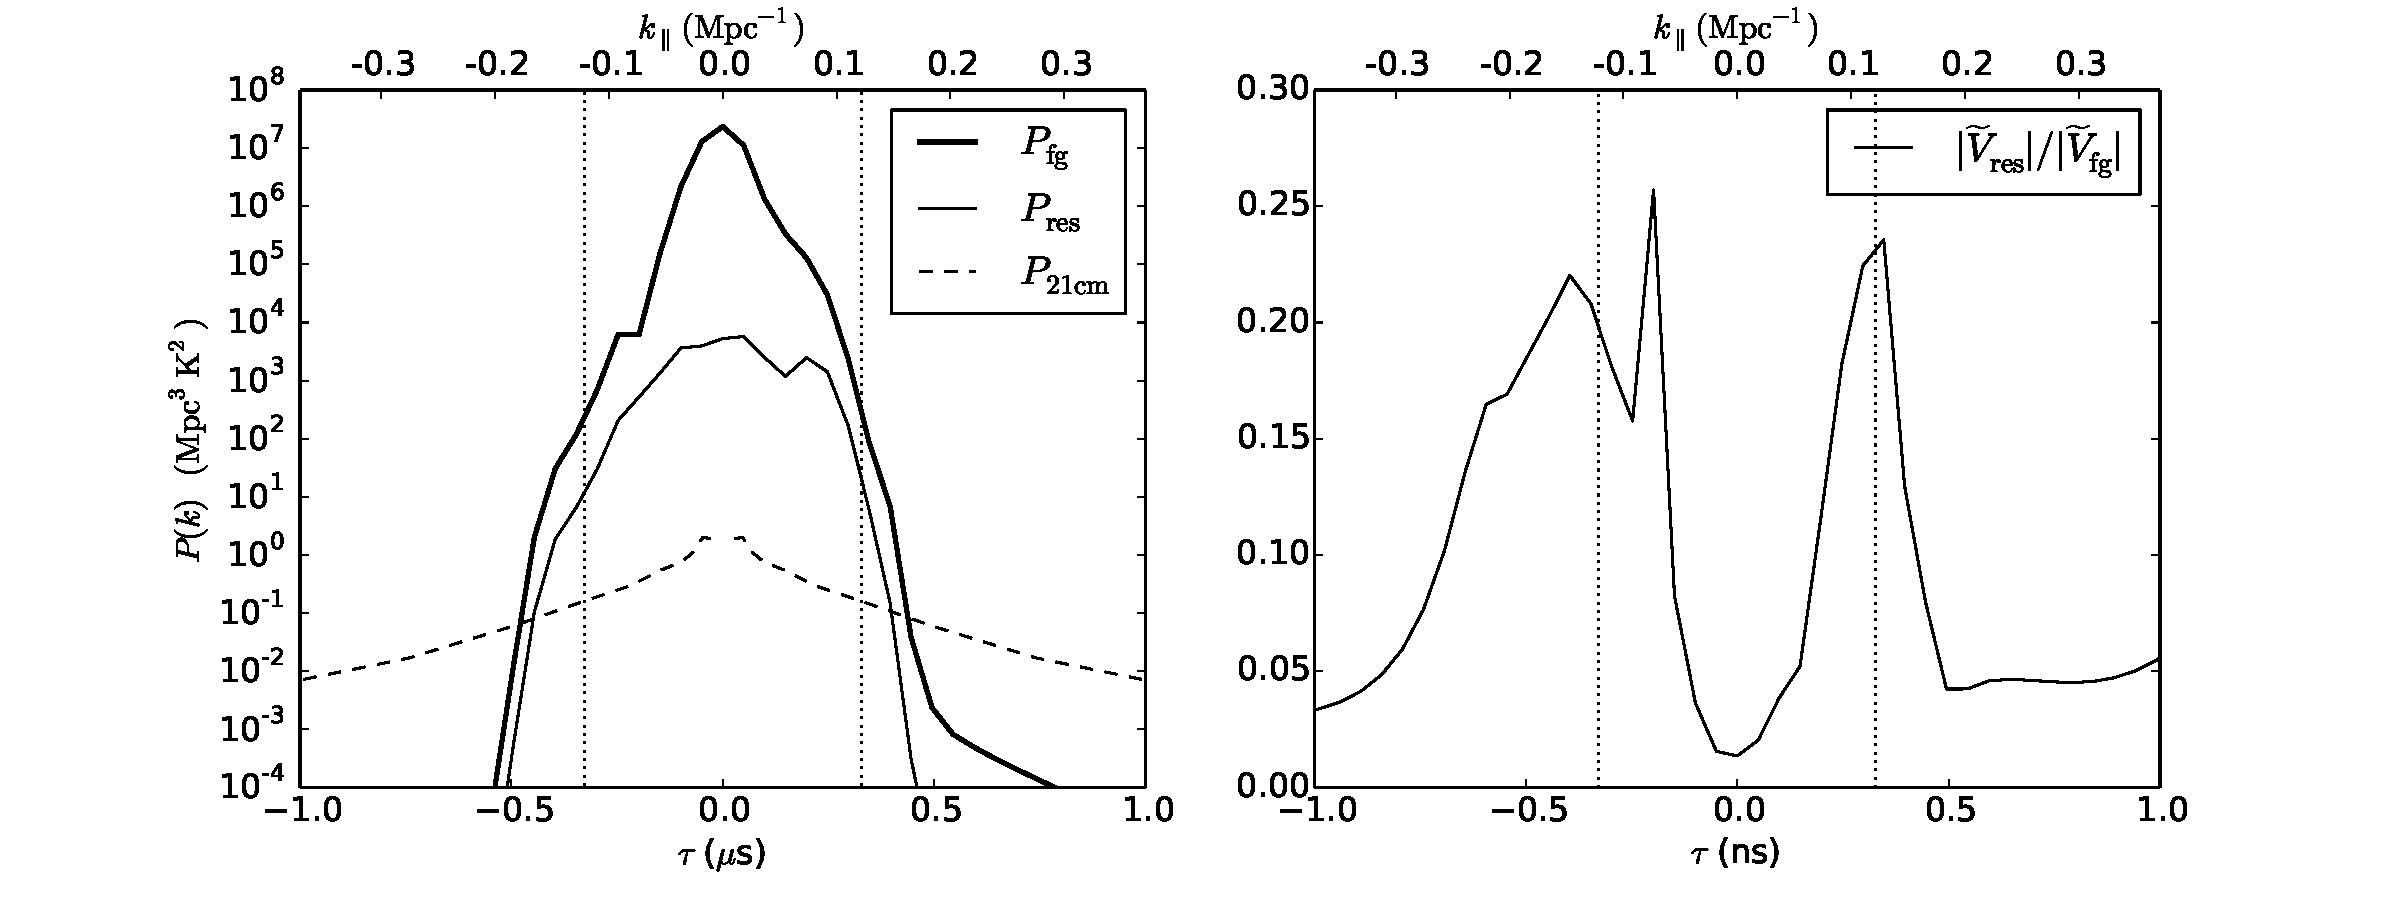
\includegraphics[width=7in]{chap2_beamforming_errors/bf_errors_in_visibilities.pdf}
\caption[Simulations of the effects of beamforming errors on foreground subtraction and avoidance techniques for a single baseline analysis.]{We simulate delay power spectra for a single baseline at 150\,MHz ($z\sim8.5$) using the Global Sky Model and point source catalogs with and without beamforming errors (dipole gain and delay errors of RMS 0.5\,dB and 50\,ps and delay slope errors of RMS 5ps/\,MHz). We use a bandwidth of 20\,MHz and a Blackman-Harris window function. Left: The total foreground power $P_\mathrm{fg}$ (thick black line) is predominantly contained within this baseline's horizon limits (vertical dotted lines) where it dominates over the cosmological signal, but falls rapidly below that signal just outside the horizon limits (the ``EOR window''). This demonstrates that the ``foreground avoidance'' approach reveals the cosmological signal even in the presence of frequency dependent beamforming errors. Measurement of the cosmological signal within the baseline's horizon limits, where it is largest, requires model subtraction with $3-4$ orders of magnitude more dynamic range in power than is achieved by subtracting an otherwise perfect foreground model with unmodeled beamforming errors $P_\mathrm{res}$ (thin black line). Right: the fractional visibility residual $|V_\mathrm{res}/V_\mathrm{fg}|$ after subtraction is largest near the baseline's horizon limits (corresponding to large zenith angles near the horizon, where the effects of beamforming errors are largest, and lowest at zero delay (in the plane bisecting the baseline and including zenith). }
\label{fig:bferrorsinps}
\end{figure*}


A power spectrum analysis diverges from an imaging analysis by incoherently averaging fourier modes (to bin different $\vec{k}$ modes into a 1D power spectrum) instead of coherently averaging them. Thus even though the effects of beamforming errors on the baseline-averaged beam are small as discussed above, further operating on the image to produce a power spectrum can make these errors very significant. Even assuming all antennas are perfectly calibrated despite the primary beam variation, sources will appear slightly brighter to some antennas and slightly dimmer to others. Subtraction of a foreground model which neglects this effect by assuming ideal beam patterns leaves residuals which vary over this spherical shell, and do not average down in the incoherent power average. 

It is these effects, as opposed to calibration effects, which we expect to be the most significant in power spectrum analysis, and to further quantify them, we simulate a power spectrum on a single baseline with and without unmodeled beamforming errors. In essence, we ask what errors would we make in a power spectrum analysis if we knew the foregrounds perfectly but lacked measurements of the exact antenna-to-antenna variation. We consider their implications for two different foreground mitigation strategies: foreground subtraction and foreground avoidance. Our simulations are centered on the MWA ``EOR0'' deep integration field, centered at R.A.(J2000) $= 0^\text{h}\,0^\text{m}\,0^\text{s}$ and decl.(J2000) $= -30^\circ\,0'\,0''$, and the sky is modeled as the sum of a deep MWA point source survey within 20$^\circ$ of the field center (Carroll et al., in prep.), the shallower but wider MWA commissioning point source survey\citep{MWACS}, the Culgoora catalog\citep{Slee1995}, and the Global Sky Model \citep{gsm}. We simulate the visibilities for a 100\,m baseline measured over a 20\,MHz bandwidth centered at 150\,MHz ($z\sim8.5$), divided into 200\,kHz channels. We do this first  assuming both both antennas in the baseline are have independent beamforming errors, and then, for an ideal beam without errors. We use beamforming errors motivated by our measurements in Figures \ref{fig:lnasplot} and \ref{fig:bf00000plot}, namely dipole gain and delay errors of RMS 0.5\,dB and 50\,ps and delay slope errors of RMS 5\,ps/MHz. As the group delay frequency-dependence is not well measured on MHz frequency scales due to our group delay window size, we intend this level of delay slope RMS as a significant overestimate of the observed delay slopes in our measurements. It is meant to set an upper limit on the effect of frequency dependent beamforming errors on the critical frequency dimension of 21\,cm measurements. We neglect tile tilt/rotation errors as Sec. \ref{sec:simulations} suggests they are subdominant to gain and delay errors. 

We plot in the left panel of Figure \ref{fig:bferrorsinps} the mean foreground power spectrum computed from 100 realizations of simulated visibilities with beamforming errors, $P_\mathrm{fg}$, and then the power spectrum after subtracting ideal model visibilities, $P_\mathrm{res}$. The delay power spectrum is computed as outlined by \citet{nithya15} using a Blackman-Harris Window function \citep{parsons12a,parsons12b}. The sky power (thick black line) dominates over the cosmological signal by typically $4-7$ orders of magnitude in power within this baseline's horizon limits (the well-known foreground ``wedge'') \citep{Dattapowerspec,X13, pober13,MoralesPSShapes, VedanthamWedge, nithya13, CathWedge, AdrianWedge1, AdrianWedge2}, but quickly drops below the cosmological signal (dashed line) \citep{21cmfast} outside these limits (in the the ``EOR window''). This demonstrates the ``foreground avoidance'' approach and shows that it reveals the cosmological signal even in the presence of frequency dependent beamforming errors. Measurement of the cosmological signal within the baseline's horizon limits, where it is largest, requires model subtraction with $2-4$ orders of magnitude more dynamic range than is achieved by neglecting beamforming errors in the foreground model (thin black line). Note that \citet{nithya15,nithya15b} observe that an increased near-horizon beam response relative to our analytic tile model tends to add a power bump at the baseline's horizon limits (the outer prongs of their ``pitchfork'').

To be sure, these residuals due to beam errors will average down somewhat when different baselines are coherently averaged in the same $\vec{k}$ cell, but $10^4-10^8$ independent samples would be needed to bring them below the level of the EOR. The maximum number of independent samples is the number of antennas in the array, each with a different realization of beamforming errors. We thus see that the coherent averaging down of beam errors in imaging power spectra is only a small effect.

To better understand these results, we plot in the right panel of Figure \ref{fig:bferrorsinps} the residual of the simulated visibilities in delay space relative to those without beamforming errors $|\widetilde{V}_\mathrm{res}/\widetilde{V}_\mathrm{fg}|$, where $\widetilde{V}$ represents the frequency fourier transform of $V(f)$. As expected, the fractional residuals are largest ($\sim$20\%) near the delays corresponding to the baseline's horizon limit (300\,ns) as these delays correspond to very low points in the beam where the effects of the beamforming errors are largest. At zero delay, corresponding to emission from the plane bisecting the baseline vector and containing zenith, the fractional residual is much lower (1.5\%). This highlights again that beam modeling errors affect preferentially the weakest beam regions which, because they are closest to the horizon, are most at risk of leaking power into the EOR window. 

\section{Discussion}

Efforts to detect neutral hydrogen emission at cosmological distances in the presence of bright galactic and extragalactic foregrounds are drawing attention to radio astronomy systematics, in particular primary beam characterization. Following up on efforts to constrain the mean MWA tile beam through advanced modeling  \citep{sutinjo15} and measurements \citep{neben15}, we explore the next order effect of antenna-to-antenna variation. We establish a budget of relevant beamforming errors and run simulations drawing from this distribution to study the effects on beam patterns. 

We characterize the beamformer paths, dipole cables, and LNAs used in the MWA tile through laboratory experiments. Summing in quadrature the group delay errors of the cables, the LNAs, and the beamformer paths, we find 46\,ps of group delay RMS, and 67ps when using the longest beamformer paths instead. This level is roughly 10\% of the beamformer shortest delay of 435ps. Gain errors appear dominated by 0.5\,dB RMS among the beamformer inputs. These errors, in addition to tile tilt/rotation errors at the $\sim0.3^\circ$ level will vary from tile to tile yielding visibility errors which do not average down with time.

We run simulations drawing from these gain, delay, and alignment errors to study the magnitude and angular-dependence of the resulting beam errors. None of these systematics is observed to have more than a percent effect on the baseline-averaged beam (the effective beam of an image) except within several degrees of the nulls. In contrast, power spectrum measurements are more sensitive to the beam standard deviations, essentially the typical tile-to-tile variation as a function of angle on the sky. Standard deviations of roughly $0.5-0.75$\,dB ($10-20\%$) are observed towards the edges of the main lobe ($20^\circ<\theta<40^\circ$) and in the sidelobes when all systematics are included (Figure \ref{fig:simall}). 

To study the effects of these beamforming errors on 21\,cm power spectrum analyses, we break down such an analysis into the different steps where beamforming errors could affect the results, and qualitatively evaluate their likely severity. They will limit calibration fidelity, though averaging in time, frequency, and over antennas can mitigate them to some extent. While the effect on the effective imaging beam will be small due to cancellation of complex visibility errors in imaging (due to \textit{coherent} combination of fourier modes), antenna-to-antenna variation will limit deconvolution accuracy nonetheless. By the same token, the effects in the power spectrum space will be larger as here different fourier modes are added \textit{incoherently} binning fourier modes into a 2D or 1D power spectrum. 

We confirm this with a simple simulation of the delay spectrum of a single visibility, addressing the question of what errors we would make in a power spectrum analysis if we knew the foregrounds perfectly but lacked measurements of the antenna-to-antenna beam variation. We find that unmodeled beamforming errors are severe enough to make foreground subtraction impossible within the baseline's horizon limits (in the wedge), where per-antenna primary beams will be necessary. However, even including an overestimate of their frequency dependence, the beamforming errors do not leak significant frequency structure into ``the EOR window'' which remains nearly clear of foreground contamination. Thus the foreground avoidance approach being pursued by PAPER, the MWA, and HERA will remain valid even in the presence of beamforming errors.

The possibility of antenna-to-antenna variation was certainly not unexpected, though measuring beams of all 128 deployed MWA antennas remains a challenge. Improved satellite-based beam calibrators and drone-based beammapping systems are under study and may make per-antenna beam measurement a reality, capturing the additional real world effects of uneven wear and tear and even failed components. Independently, future work will extend simulations by \citet{nithya15} to include per-antenna beamforming errors and propagate them from measured visibilities through calibration, imaging, and power spectrum analysis to definitely address their effects on 21\,cm science for the MWA. 

Building on lessons learned from development of the MWA and PAPER, HERA is pursuing a targeted experiment to detect the cosmological signal using zenith-tracking dishes rather than phased arrays, and foreground avoidance rather than the more challenging subtraction. In contrast, observatories relying both on beamforming and foreground subtraction (e.g., LOFAR and SKA-Low) must model the sky and primary beams (either through calibration or measurement) to four to five orders of magnitude of dynamic range lest foreground residuals swamp the feeble cosmological signal.

\begin{subappendices}

% in depth description of the MWA tile
\section{Appendix: Design of the MWA Antenna Tile}

\subsection{Design and Science Requirements}
Redshifted hydrogen line emission from the Epoch of Reionization ($6\lesssim z\lesssim12$) appears in the 100-200\,MHz band, several orders of magnitude fainter than galactic and extragalactic radio emission. Separating this high redshift signal from foregrounds is thought to be possible by exploiting their different frequency dependence. While the foregrounds result from smooth spectrum radio synchrotron emission, the frequency axis of the signal is actually a cosmological redshift axis, and thus probes the complex spatial structure of the ionizing universe. Instrumental noise also plays a key role, and its mitigation necessitates large collecting area.

These science goals informed the instrumentation requirements as follows. The desired frequency band represents an order unity fractional bandwidth, necessitating a wideband antenna with a smooth frequency response. In particular, significant frequency structure on scales smaller than the nominal power spectrum analysis bandwidth of 10\,MHz (set by timescale of $\Delta z\sim0.5$ over which the cosmological signal is expected to evolve) would complicate beam modeling and risk smearing smooth spectrum foregrounds into spectrally noisy signal-like modes. A large field of view, in comparison to more traditional radio telescopes like the Very Large Array, is also desired to maximize the cosmological volume over which to measure the EOR power spectrum. Instrumental noise is minimized to the sky noise limit through use of low noise amplifiers (LNAs) placed as early in the signal chain as possible. A steerable beam was also desired to allow deep observing on discrete patches of sky, and thus coherent integration on power spectrum modes. This strategy reduces noise much more quickly with integration time at the expense of an increase in cosmic variance noise \citep{TrottObservingModes}. Lastly, and arguably most importantly, is the large required collecting area at modest cost, achieved with an array of order one hundred low cost ($\lesssim\$2500$/ea) antenna elements. The MWA is a realization of the ``Large N--Small D'' array concept consisting of a large number of small diameter antenna element made possible by advances in parallel computer processing. 

Though it is tuned to some extent to achieve the high surface brightness sensitivity required by EOR science, this design also permits a host of other low frequency science ranging from transient searches and source surveys to solar and ionospheric science \citep{mwascience}. The MWA tile design is, therefore, a compromise to meet different science goals. Further optimization for EOR science is possible, for example, HERA, is pursuing larger antenna elements to increase sensitivity without extra computing cost. At the array level, the HERA antennas will be positioned on a regular grid to achieve many redundant baselines, and thus allow coherent integration on individual power spectrum modes.

\begin{figure*}[h]
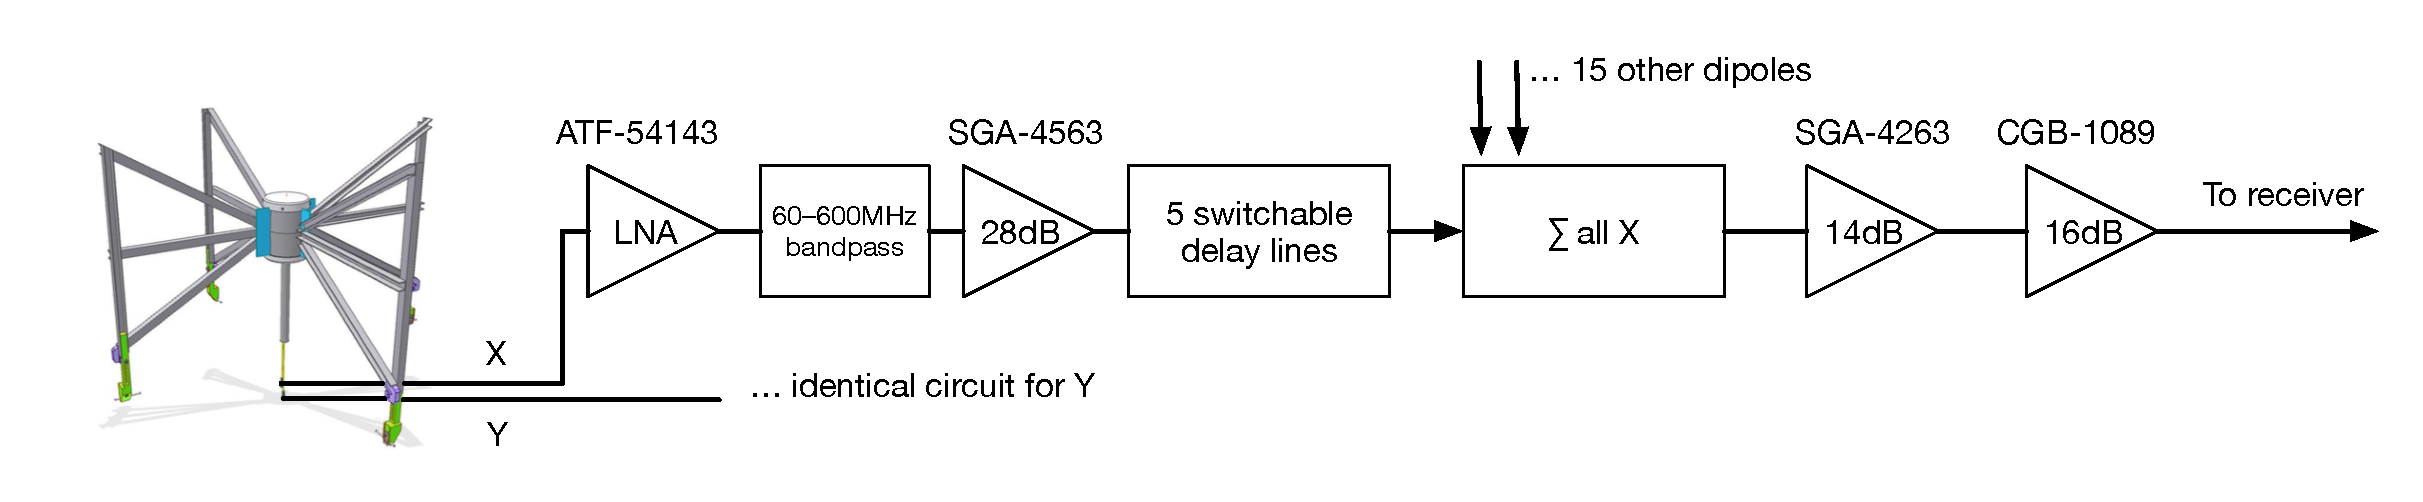
\includegraphics[width=7in]{chap2_beamforming_errors/beamformer_signal_path.pdf}
\caption[Beamformer signal path.]{For each polarization, each of 16 dipole signals passes through a balun/LNA (represented by the first amplifier in the diagram) mounted in the dipole hub with a gain varying between 16--25\,dB across the band. The signal is then carried into the beamformer, where it goes through a low pass filter, an amplifier, 5 switchable delay lines, a series of two-way power combiners which sums the 16 dipole signals, then two more amplifiers. The delay lines are replaced by matching attenuators when disengaged. Walsh switching may be implemented directly after the power combiners. Driving just one beamformer input, the gain totals roughly 33\,dB at 150\,MHz accounting for losses in the power combiners and other components. }
\label{fig:beamformersdiagram}
\end{figure*}

\subsection{Dipole Element}

Each MWA dipole element is a set of two orthogonally crossed vertical bowties, each of length 74\,cm and height 38\,cm. Each bowtie is composed of two aluminum arms mounted at a PVC hub such that the lowest part of the antenna is 8\,cm above the ground screen. In principle, an infinite bowtie antenna has infinitely broad bandwidth because it has no characteristic length scale. A real bowtie is truncated, which introduces length scales and resonances, but the bandwidth remains broad and the response generally smooth on frequency scales of interest. 

Note that despite the arms not being composed of solid metal sheets, the electrical performance of our bowtie differs negligibly from that of a more costly solid one while also mitigating wind loading. Other dipole style antennas were modeled in various orientations, but the bowtie was chosen for its relatively smooth gain over frequency, minimum gain variation over elevation, low horizon gain, absence of blind spots or other anomalies in the patterns or impedance, and impedance match with the LNAs.

One unexpected discovery was made during early antenna testing relating to coupling between adjacent dipoles in a tile. Interactions between the vertical pieces in a row or column of dipoles direct power towards the horizon in much the same way that one attaches perpendicular arms to a metal rod to form a directive Yagi antenna. Consequently, the dimensions of the antenna were adjusted to the present values to move this resonance to 240\,MHz, near an already unusable satellite band. 

Inside each PVC hub is a dual-polarization low-noise amplifier (LNA) that also serves as a balun between the balanced bowtie terminals and the 50\,$\Omega$ coaxial cable to the beamformer. In detail, there is an amplifier on each of the four dipole arms. The amplified signals from opposing arms are combined through a center-tapped transformer balun to feed a 50\,$\Omega$ unbalanced coaxial cable.The LNA gain with a 50\,$\Omega$ source is $\sim$19\,dB at 150\,MHz. The impedance match with the sky is sufficient to make the system sky noise dominated. Quality control data on the field-deployed dipole LNAs is collected periodically in an array dipole testing mode during which the beamformer paths are all switched off, then each is switched on individually. The LNAs are powered with a 5\,V DC bias provided by the beamformer on the 7\,m LMR-100 cables (50$\Omega$) which also carry the sky signals in the opposite direction. In their deployed configuration, these cables are fixed with wire ties atop the ground screen. 

\subsection{Ground Screen}
\label{sec:groundscreen}
The 5\,m $\times$ 5\,m ground screen is formed by three overlapped 2\,m $\times$ 5\,m mesh panels welded together and laid directly on the ground. Each panel is constructed of 3.15\,mm galvanized steel wire, welded together to form a grid of 50\,mm $\times$ 50\,mm squares. Typical dipole position errors are at the 5\,mm level or smaller on average throughout the dipole grid, due to mesh thickness and distortions due to handling, and also slightly larger errors overlapping the different mesh panels. Such horizontal errors are irrelevant for radiation incident from zenith, but contribute per-dipole delays up to an RMS of approximately 17\,ps towards the horizon due to the altered light travel time to the different elements. In any case, these errors are subdominant to other errors discussed below.

No large or small scale ground leveling was attempted, but the flatness and alignment estimated with  differential-GPS measurements is better than a few cm vertically and $\sim1^\circ$ in alignment with North and zenith. We discuss this alignment precision in more detail in Sec. \ref{sec:measurements}. An electrical path to ground is provided through a connection to the wire chassis of the beamformer and subsequently to the receiver, itself grounded to metal ground stakes.

\subsection{Beamformer}
The beamformer contains two vertically offset delayline boards, one for each polarization, each fed by 16 dipole inputs. Each input is directed through a series of digitally switchable delay lines before being summed with the others with specified relative delays applied, and output to the receiver. Figure \ref{fig:beamformersdiagram} shows a block diagram of the signal path. Each input passes through a 4-pole lowpass filter with a 3\,dB cutoff at 600\,MHz, a 30\,dB amplifier, five sequential switched delaylines, a switch that either passes the signal or terminates with 50\,$\Omega$, and lastly a cascade of two-way power combiners which sum the 16 inputs. Note that this low pass filter serves simply to protect the analog components from saturation; there is a second low pass anti-aliasing filter in the receiver. The shortest delay line is 435\,ps, a number determined by the requirement that the beam be steerable to $30^\circ$ elevation with five delay line ``bits'' whose electrical lengths form a geometric series with a ratio of 2. These boards are also capable of applying Walsh switching to the summed signal to mitigate cross-coupling between different signal paths from different MWA tiles, though this feature has not been found to be necessary and has not been implemented. 

Digital communication to the beamformer to activate delay bits on each of the delay lines is transmitted in a ``data over coax'' configuration, multiplexed on the two RG-6 cables carrying the dual-polarization beamformer output to the receiver. 

\end{subappendices}

\section*{Acknowledgements}

This work was supported by NSF grant AST-0821321, the Marble Astrophysics Fund, and the MIT School of Science. We thank Aaron Ewall-Wice and Hamdi Mani for assistance in running these experiments, Steve Burns for debugging beamformer issues, and Danny Jacobs, Nithyanandan Thyagarajan, and Lu Feng for helpful discussions. 

This scientific work makes use of the Murchison Radio-astronomy Observatory, operated by CSIRO. We acknowledge the Wajarri Yamatji people as the traditional owners of the Observatory site. Support for the MWA comes from the U.S. National Science Foundation (grants AST-0457585, PHY-0835713, CAREER-0847753, and AST-0908884), the Australian Research Council (LIEF grants LE0775621 and LE0882938), the U.S. Air Force Office of Scientific Research (grant FA9550-0510247), and the Centre for All-sky Astrophysics (an Australian Research Council Centre of Excellence funded by grant CE110001020). Support is also provided by the Smithsonian Astrophysical Observatory, the MIT School of Science, the Raman Research Institute, the Australian National University, and the Victoria University of Wellington (via grant MED-E1799 from the New Zealand Ministry of Economic Development and an IBM Shared University Research Grant). The Australian Federal government provides additional support via the Commonwealth Scientific and Industrial Research Organisation (CSIRO), National Collaborative Research Infrastructure Strategy, Education Investment Fund, and the Australia India Strategic Research Fund, and Astronomy Australia Limited, under contract to Curtin University. We acknowledge the iVEC Petabyte Data Store, the Initiative in Innovative Computing and the CUDA Center for Excellence sponsored by NVIDIA at Harvard University, and the International Centre for Radio Astronomy Research (ICRAR), a Joint Venture of Curtin University and The University of Western Australia, funded by the Western Australian State government.






\chapter{The HERA Dish: Beam Measurements and Science Implications}
\label{chap:herapaper}
The content of this chapter was originally published as Neben, A.R. et al., \textit{The Hydrogen Epoch of Reionization Array Dish. I. Beam Pattern Measurements and Science Implications}, ApJ, 826:199, 2016. Dave DeBoer and Richard Bradley led the team at Green Bank that assembled the prototype HERA dish, and they each ran numerical electromagnetic models of its beampattern. I operated our beam measurement experiment, collected the data, synthesized it into beam patterns, and fed back to Dave and Rich on how to modify the dish. I also did my own simulations of the effects of model deviations on foreground mitigation for HERA, and worked with Nithya Thyagarajan understand simulation artifacts. I wrote the paper on our results. \\

The Hydrogen Epoch of Reionization Array (HERA) is a radio interferometer aiming to detect the power spectrum of 21\,cm fluctuations from neutral hydrogen from the Epoch of Reionization (EOR). Drawing on lessons from the Murchison Widefield Array (MWA) and the Precision Array for Probing the Epoch of Reionization (PAPER), HERA is a hexagonal array of large (14\,m diameter) dishes with suspended dipole feeds. Not only does the dish determine overall sensitivity, it affects the observed frequency structure of foregrounds in the interferometer. This is the first of a series of four papers characterizing the frequency and angular response of the dish with simulations and measurements. We focus in this paper on the angular response (i.e., power pattern), which sets the relative weighting between sky regions of high and low delay, and thus, apparent source frequency structure. We measure the angular response at 137\,MHz using the ORBCOMM beam mapping system of \citet{neben15}. We measure a collecting area of 93\,m$^2$ in the optimal dish/feed configuration, implying HERA-320 should detect the EOR power spectrum at $z\sim9$ with a signal-to-noise ratio of 12.7 using a foreground avoidance approach with a single season of observations, and 74.3 using a foreground subtraction approach. Lastly we study the impact of these beam measurements on the distribution of foregrounds in Fourier space.

\section{Introduction}
%- basics of 21cm cosmology
%    - shedding light on the unobserved Dark Ages and Epoch of
%      Reionization when the first luminous sources formed and reionized
%      the IGM
%    - MWA, PAPER, LOFAR, GMRT power spectrum experiments
%    - also global signal experiments like XX,YY,ZZ,
%        - the big challenge is recovering the signal below 4-5 orders of
%      magnitude brighter foregrounds and noise
%    - naive requirement is collecting area
%    - naive foreground removal is to subtract all low $k_\parallel$ modes

A new generation of low frequency radio telescopes is coming online with the goal of
 probing redshifted 21\,cm emission from the Cosmic Dawn. These observations will 
 complement indirect probes of the Epoch of Reionization such as quasar 
 sightlines and the CMB optical depth, which leave the reionization 
 history of the universe only loosely constrained. (See \citet{FurlanettoReview, miguelreview, PritchardLoebReview, aviBook, zaroubi} for reviews) In the longer term, 21\,cm observations are expected to improve constraints on cosmology \citep[e.g.,][]{mao08, liu15a,liu15b}. Sensitivity and foreground removal are 
 the main challenges in 21\,cm observations, as the expected cosmological signal is 4--5 
 orders of magnitude fainter in brightness temperature than Galactic and extragalactic foregrounds. Radio 
 interferometers such as the Murchison Widefield Array (MWA) \citep{lonsdale09,tingay13,mwascience}, the Precision Array for Probing the Epoch of Reionization (PAPER) \citep{parsons10,parsons14,ali15}, the Giant Meterwave Radio Telescope (GMRT) 
 \citep{Paciga2011}, and the Low Frequency Array (LOFAR) \citep{lofar} are seeking a first detection of 
 cosmological 21\,cm emission in power spectrum measurements. In the power spectrum, the spectrally smooth foreground emission separates from the spectrally 
 rough cosmological signal whose frequency dimension probes a line of sight through the 
 inhomogenous reionizing universe.


The Hydrogen Epoch of Reionization Array (HERA) \citep{PoberNextGen,deboer16} is drawing on lessons learned by the MWA and PAPER to reach the calibration and foreground isolation accuracy required to make a significant detection and characterization of the cosmological signal. HERA uses 14\,m diameter parabolic dishes arranged in a compact, hexagonal array to achieve coherent integration of the very low surface brightness 21\,cm signal. Redundant baselines also permit redundant calibration techniques which solve for the relative calibration between all antennas \citep{redundant3, redundant4, liu10,zheng14}. A central lesson from first generation instruments is that it is essential to characterize the instrument response to foreground emission lest instrument frequency dependence smear foreground power into cosmological signal modes. 

%%- but instrumental frequency structure has been recognized as critical
%  => wedge
%    - of course the bandpass and intrinsic smooth freq structure of
%      sources
%    - but also the freq-dependent sampling of the IFO
%    - sources at different zenith angles appear at different delays,
%      and thus different $k_\parallel$, increasing linearly with baseline length
%    - this gives rise to the “wedge” in cylindrically averaged power
%      spectra ($k_\perp$, $k_\parallel$)

In an ideal achromatic instrument the foreground emission would be confined to the lowest few 
line of sight Fourier modes \citep[e.g.,][]{MoralesBowmanHewittFGsub}, however  the  
interferometer's frequency-dependent point spread function smears foreground power into a ``wedge'' shaped 
region in $(k_\perp,k_\parallel)$ Fourier space \citep{Dattapowerspec,X13, pober13,MoralesPSShapes, VedanthamWedge, nithya13, CathWedge, AdrianWedge1, AdrianWedge2,parsons12b}, where $k_\parallel$ modes are along the line of sight and $k_\perp$ modes are perpendicular to it. This effect is straightforward to understand for a single baseline which measures the sky intensity weighted by the complex sky fringe 
$e^{2\pi i \nu \tau_g}$, where $\tau_g=\vec{b}\cdot\hat{s}/c$ is the delay in radiation arrival time at the second antenna relative to the first antenna of the baseline. Here $\nu$ is the observation frequency, $\vec{b}$ is the baseline vector, and $\hat{s}$ is the direction of the source. 
 Thus sources at different positions relative to the baseline vector appear with different 
frequency structure despite their intrinsically smooth spectra. However, this instrumental frequency structure is limited 
by the baseline length to a maximum frequency dependence of  $e^{2\pi i \nu b/c}$ for sources at maximum delay, near the horizon in line with the baseline vector. This limits the foreground contamination 
to a wedge shaped region in Fourier space with $k_\parallel<a k_\perp$, where $k_\perp$ and $k_\parallel$ represent spatial modes 
perpendicular and parallel to the line of sight, and $a$ is a constant depending on the observational frequency and cosmology. The complement of the wedge is known as the ``EOR window''.

So because sources acquire frequency dependence based on their position on the sky, and the primary beam weights different regions of the sky differently, we see that the primary beam (i.e., the antenna angular response) strongly affects the aggregate frequency dependence 
of the foregrounds. \citet{nithya15} simulate the foreground contamination seen with a dipole beam, a phased array, and a Airy pattern,
and find that the latter suffers the least foreground leakage into
 $k_\parallel>0$ modes due to its narrow main lobe and minimal sidelobe 
levels. To be sure, all are subject to the same geometric limits on foreground frequency-
dependence which limit foreground bounding foreground emission within the wedge, but the emission from high delay is better suppressed using the 
Airy pattern leaving much of the wedge effectively empty. 

%%- the beam affects the wedge
%    - Nithya et al quantify the effects of antenna beam on the wedge
%    - wider beams like the dipole have large response at large zenith
%      angle, and thus large delays, wedge much more filled out, and
%      much more emission close to the EOR window, at risk of leaking in
%    - narrower beams like the airy have much narrower response, most
%      received emission is from low delays (near $k_\parallel=0$)
%    - but even there, emission is seen at the edge of the wedge,
%      interpreted as an effective brightening of the horizon due to the
%      very large solid angle it subtends 
%    - this structure (lots of emission from zero delay, and peak at the
%      horizon), was termed the pitchfork
%    - highlights importance of beam characterization across the entire
%      sky

For foreground avoidance-based power spectrum estimation, so long as foreground emission is perfectly contained in the wedge it is irrelevant how much or 
little of it there is, but real world effects smear power beyond the geometrical edge of the wedge into the EOR 
window. Finite bandwidth, imperfect bandpass calibration, and faraday rotation of polarized sources can all imprint slight frequency structure on otherwise spectrally smooth sources \citep{jelic2010,bernardi13, moore13,moore15,asad15,newburgh14,shaw15}, and those closest to the edge of the wedge are 
most at risk of leaking into the EOR window. In fact, 
\citet{nithya15,nithya15b} observe in simulations and then in data that while naively we might expect minimal emission 
at the very edge of the wedge because typical near-horizon beam responses are so small, 
two effects can cause a relative brightening of emission at those maximal delays, creating a characteristic ``pitchfork'' shape. This horizon 
brightening is caused by the large solid angle subtended by the near-horizon regions of the 
sky, as well as the apparent shortening of baselines when viewed nearly on axis at these elevations. 
This second effect makes intermediate length baselines of tens to hundreds of meters sensitive to the very bright diffuse 
emission they would not see from near zenith. Together, these effects can overcome the decline in beam sensitivity near the horizon. 
All these considerations highlight the antenna beam as a critical design parameter for 
21\,cm observatories.

%%- the design of the HERA dish
%    - small D, large N technique was enabled by moore’s law
%    - even if processing hundreds to thousands of hours of data on
%      order hundred of antennas is technically possible with parallel
%      processing and advanced data quality metrics
%    - first generation experiments are aiming for a first detection of
%      the power spectrum, even more sensitivity will be needed to
%      characterize its evolution with redshift and k, and test models
%    - HERA has thus opted for larger elements, at the expense of a
%      smaller FOV, but most of our fourier modes come from freq
%      dimension anyway
%    - a dish is preferred to a large phased array (a la SKA) as a
%      simpler antenna, with fewer degrees of freedom and reduced
%      potential for ant-to-ant variation (Neben et al)
%    - of course, elevating a feed above a dish introduces potential for
%      reflections, and thus a wigglier bandpass than that of the MWA or
%      PAPER
%    - The other papers in this series set a wiggliness spec and present
%      measurements showing it meets the spec
%    - here we focus on the angular response of the dish, ie, its beam
%      pattern


This is the first in a series of four papers detailing the HERA element. In this work we study 
the angular response of the dish and its implications for power spectrum measurements. The three companion 
papers present reflectometry measurements \citep{patra16} and simulations \citep{ewallwice16} of the dish frequency response, as well as detailed 
foreground simulations for HERA \citep{nithya16}. A general description of the design of the 
HERA experiment is given by DeBoer et al. \citep{deboer16}. In essence, we 
require a large collecting area for
 sensitivity, and minimal sidelobes and horizon response without incurring the large cost per collecting 
area of very large dishes. A dish is preferred to a large phased array as it has a less complex beampattern and reduced potential for antenna-to-antenna variation \citep{neben16}. The core array consists of 320 dishes positioned on a compact, hexagonal 
grid \citep{dillonparsons16} permitting redundant baseline calibration and coherent integration in $
\vec{k}$ space \citep{zheng14,parsons12a}. Improved imaging is permitted by 30 outriggers, but these do not appreciably affect power spectrum sensitivity.
%The smaller field of view of the HERA dish relative to that of the PAPER dipole or the MWA tile does not limit sensitivity in Fourier space as most leverage on high $k$ modes is from line of sight modes anyway \citep{PoberNextGen}.

%%- roadmap
%    - we use orbcomm to measure the dish beam pattern and calculate
%      collecting area, verify the focus
%    - then we assess the science implications in delay space, comparing
%      different models and power spectrum approaches
%%- how sensitive are we to accurate beam models?
%    - what must we show about the HERA dish to confirm that it will
%      allow us to reach the science we want?
%    - large collecting area is a given
%    - minimal sidelobes and horizon response
%    - how accurately must we verify the beam model? different analyses
%      require different levels of beam modeling fidelity
%    - HERA’s hexagonal grid permits redundant baseline calibration
%      which is agnostic to the antenna beam, as long as all are the
%      same. ant-to-ant variation adds noise to the redundant
%      calibration, likely much smaller than that incurred in MWA sky
%      model calibration 
%    - the PAPER delay spectrum technique and 1D clean is even agnostic
%      to ant-to-ant variation, as it cleans out all sky emission within
%      the horizon limits on a per baseline basis
%    - an imaging analysis (a la MWA) relies on foreground subtraction,
%      and containment of residuals in the wedge, and the subtraction
%      step is much more sensitive both to accurate modeling of the mean
%      beam and to ant-to-ant variation (Neben et al)
%    - the general questions we address in this paper
%        - the questions are: does the main lobe shape agree with the
%          model (need good model for imaging and FG subtraction)
%        - are the sidelobe levels and horizon response sufficiently
%          small to mitigate pitchfork effect and foreground leakage?

In this paper we first characterize the angular response of a prototype HERA dish at the National Radio 
Astronomy Observatory--Green Bank. We use the beam mapping system of \citet{neben15} to 
measure the 137\,MHz beam pattern using the ORBCOMM satellite constellation. We obtain beam 
measurements out to zenith angles of $\sim60^\circ$ where the beam response is -35\,dB relative to zenith, and compare with different numerical electromagnetic models. We characterize the dish beam at various feed heights to map out the focus and study beam errors due to feed misalignment. We compute the collecting areas and implied EOR power spectrum sensitivities of our measured beams. After verifying our models, we consider the science implications of these 
beam patterns by foreground delay spectra at different baseline lengths and observing conditions to study when the horizon brightening effect is strongest, and thus, when foregrounds are most at risk of leaking into the EOR window.

We discuss the electromagnetic design and modeling of the dish in Section 2. We present the 
experimental setup of the beam mapping experiments and discuss their systematics, then 
review the ORBCOMM beam measurement system in Section 3. We present our power pattern 
measurements in Section 4, and study the science implications of these beam measurements for foreground power spectra in Section 5, then conclude with discussion in Section 6.

\section{Dish Design and Modeling}

\subsection{Design of the HERA Dish}

The HERA element (Fig. \ref{fig:feeddiagram}) is a 14\,m diameter faceted paraboloid ($ f/D=0.32$) with a dual-polarized dipole feed suspended at prime focus \citep{dishmemo}. Here $f$ is the focal length of the dish and $D$ is the dish diameter. The dish surface is formed by wire mesh sheets (i.e., facets) mounted on PVC tubes which run from the lip of the dish to the hub at the vertex. For these tests, the feed consists of a dual linear polarization PAPER sleeved dipole mounted 17'' below a 78'' diameter wire mesh back plane surrounded by a 30'' deep cylinder. The feed is suspended from a single point on its back plane from three ropes, each attached to a telephone pole. The three telephone poles are equally spaced around the dish. The dipole ``sleeves'' are circular disks just above and below the dipole designed to broaden its frequency response. The feed cylinder is offset 0.5'' from the back plane, and is designed to make the dipole beam more azimuthally symmetric and also taper its response near the edges of the dish to reduce spillover into adjacent dishes. Fig. \ref{fig:feedphoto} shows the feed as deployed on the ground for early testing. 

The nominal dish focus is $f=(f/D)D=4.48$\,m, though given its faceted design, the dish does not have a single focus. Our numerical electromagnetic models suggest the best focus is slightly higher than that of an perfect paraboloid. In this work we study the dish beam pattern at rigging heights of 4.5\,m, 5.0\,m, and 5.3\,m, measured from dish surface to feed plane, the last height being the maximum height we can achieve with the feed suspension system installed on the dish. These height measurements are uncertain at the $\pm5\%$ level in this study. For more details on the dish design and construction see \citet{deboer16}. Feed optimization studies are ongoing and the values of these parameters may change in the full HERA array \citep{feedoptimizationmemo}. 

\begin{figure}[h]
\centering
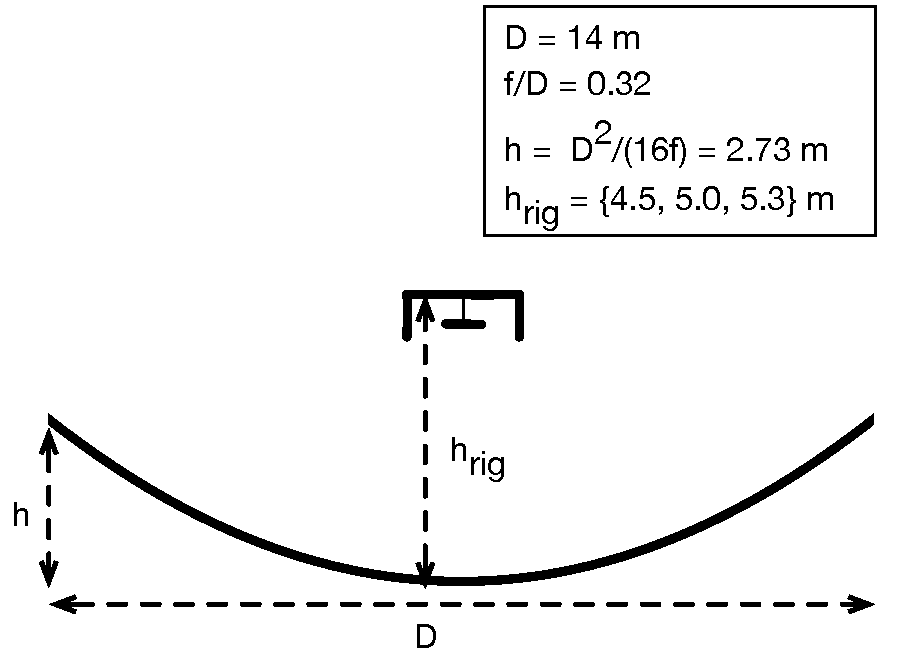
\includegraphics[width=3.4in]{chap3_hera_beammapping/dish_and_feed_diagram.pdf}
\caption{Diagram showing the dimensions and layout of the parabolic HERA dish and suspended feed.}
\label{fig:feeddiagram}
\end{figure}

\begin{figure}[h]
\centering
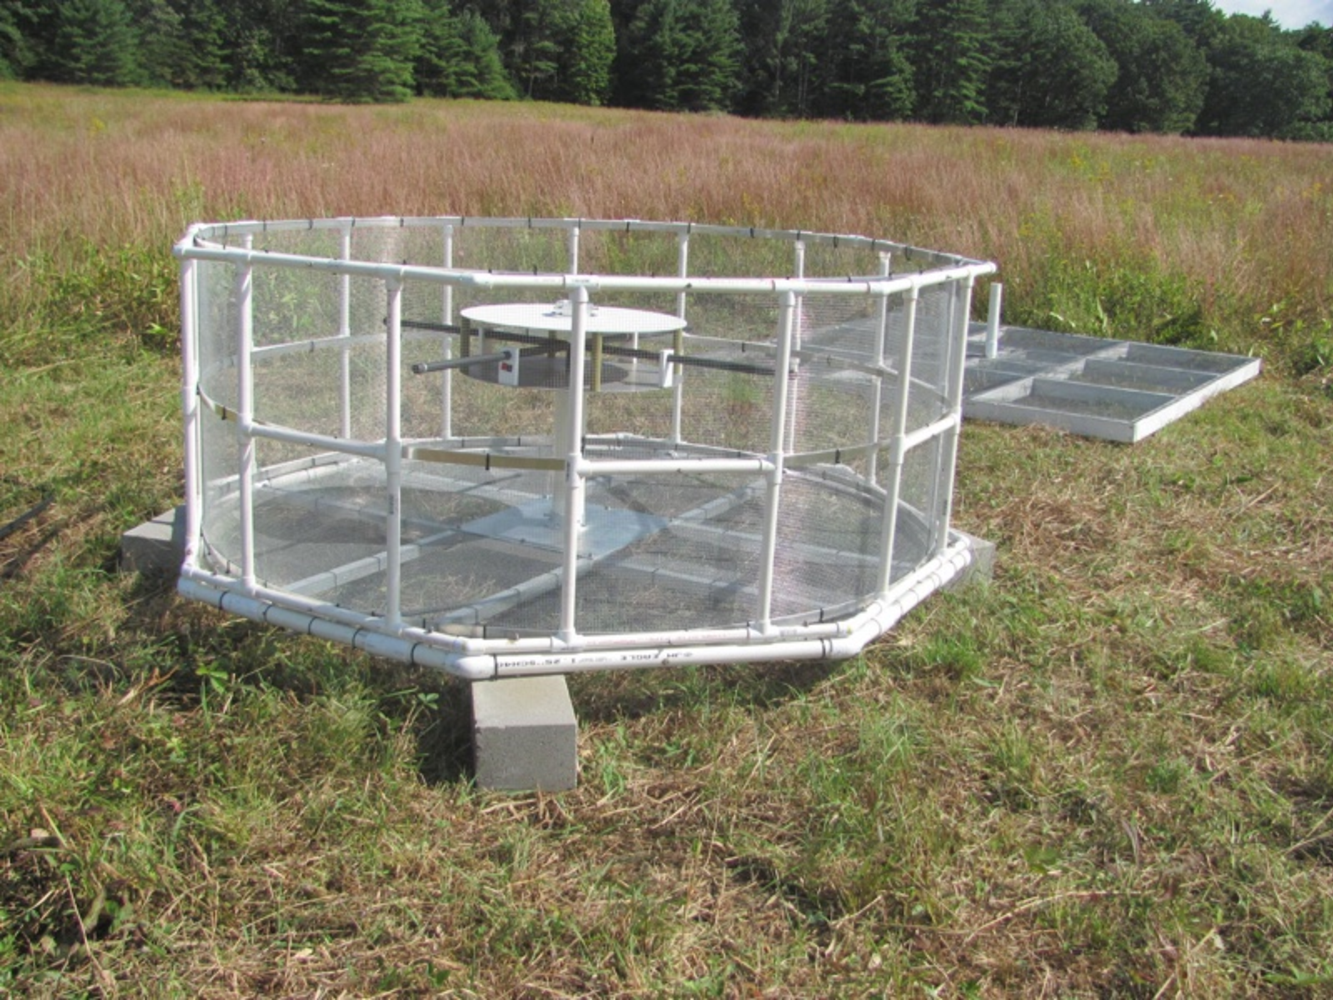
\includegraphics[width=3.4in]{chap3_hera_beammapping/feed.pdf}
\caption[Prototype HERA feed seen here outside the dish and upside-down for preliminary characterization.]{Prototype HERA feed seen here outside the dish and upside-down for preliminary characterization. This feed revision consists of a dual-polarized sleeved dipole offset 17'' from a 78'' diameter back plane, surrounded by a 30'' deep cylindrical skirt.}
\label{fig:feedphoto}
\end{figure}

As the HERA element is larger than the MWA or PAPER antenna elements, one might worry about the  smaller field of view and thus smaller range of Fourier space probed perpendicular to the line of sight. However, this is a 
small effect for 21\,cm power spectrum analyses as our leverage on $k$ modes comes primarily from modes along the line of sight (in the frequency dimension). Further, HERA's smaller field of view is actually desirable in that it drastically reduces the magnitude of emission at the edge of the wedge compared to a simple dipole element \citep{nithya15}. A second potential drawback is frequency structure introduced by time domain reflections between the dish and feed detailed by Ewall-Wice et al. \citep{ewallwice16} with simulations and \citep{patra16} with zenith reflectometry measurements. These works demonstrate, though, that the slight frequency structure of the dish is sufficiently small to not interfere with EOR science.

\subsection{Dish Modeling}
\label{sec:dishmodels}

\begin{figure*}
\centering
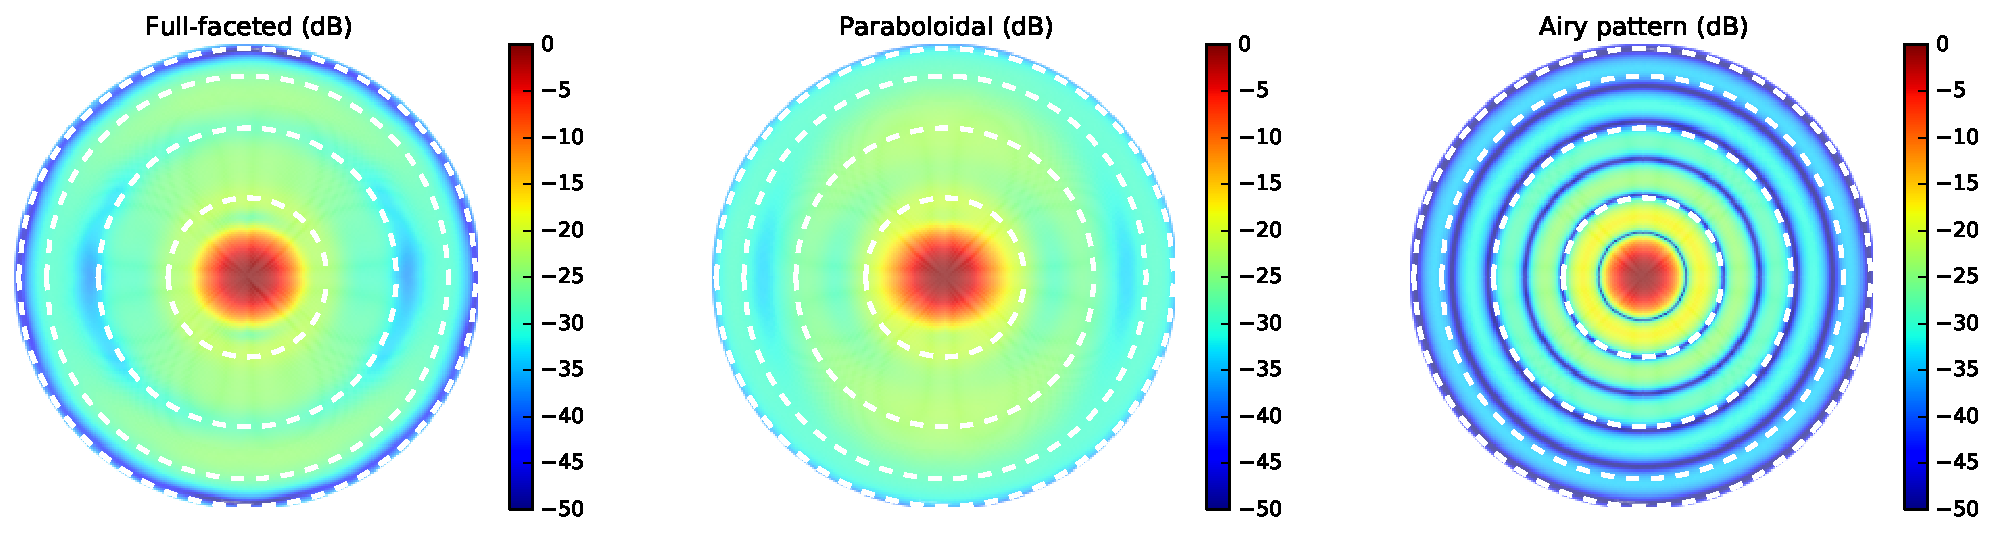
\includegraphics[width=6in]{chap3_hera_beammapping/dave195_rich195_airy_beams.pdf}
\caption[Simulated dish power patterns.]{Simulated dish power patterns (NS polarization) at 137\,MHz (see Sec. \ref{sec:dishmodels}) with $h_\text{feed}=5$\,m using the full-faceted model (left) and the perfect paraboloidal model (middle) are shown beside an ideal Airy pattern for a 14\,m diameter dish for comparison. Dased lines mark zenith angles of 20$^\circ$, 40$^\circ$, 60$^\circ$, and 80$^\circ$.}
\label{fig:modelbeams}
\end{figure*}

We numerically model the HERA dish in two different ways in order to study the range of realistic beams given modeling inaccuracies and material imperfections. In particular, the near horizon beam response, which sets the level of horizon brightening in the delay spectrum, is quite sensitive to modeling assumptions. We first generate a full-faceted model of the dish using ANSYS HFSS\footnote{http://www.ansys.com/Products/Electronics/ANSYS-HFSS}. All mesh surfaces are modeled as solid aluminum and the dipole itself is modeled as copper. The 1\,m concrete circle at the vertex is modeled with a dielectric similar to dry soil. For comparison, we also model the dish as a perfect paraboloid. We simulate this second model using CST Microwave Studio\footnote{https://www.cst.com/Products/CSTMWS}, but the differences are dominated by the dish geometry, not the choice of numerical electromagnetic solver. 

The simulated full-faceted and perfect paraboloid beams for the NS dipole are plotted in Fig. \ref{fig:modelbeams} (left and center panel) along with an Airy pattern for comparison. As expected, both model beams have slightly stronger sidelobes and wider main lobes than the ideal Airy pattern. The dipole sleeve (circular pieces in Fig. \ref{fig:feedphoto}) and skirt result in a feed beam which is slightly elongated in the E plane and slightly compressed in the H plane, opposite to the behavior of a simple dipole. This wider dish illumination in the NS direction by the NS feed dipole results in a narrower dish beam in the NS direction. Similarly, the EW dish beam is narrower in the EW direction. Lastly, we note that in both models, the best focus is found to be close to 5.23\,m with this feed geometry.

\section{Experimental Setup}

\subsection{ORBCOMM Beam Mapping System Review}
\label{sec:orbcommreview}

We briefly review the beam mapping system detailed by \citet{neben15}, then discuss the 
application of the system for HERA dish measurements. The system 
takes advantage of the 137\,MHz communications satellites operated by ORBCOMM Inc. 
as bright point sources which, by virtue of their number ($\sim30$), short orbital periods 
($\sim90$ minutes), and orbital precession, cover $\sim$65\% of the visible sky in just a few 
days. The coverage from the Green Bank site is limited by the fact that the satellites' orbital inclinations are all less 
than $45^\circ$. 

Unlike celestial source beam measurements, where the flux may be 
assumed constant over the timescale of the measurement, satellite fluxes can vary rapidly 
due to changing distance, orientation, and transmission power. To correct for this, we 
measure the satellite flux in each ground polarization (East-West (EW) and North-South (NS)) using a simple, well-
modeled reference antenna. Comparison of this measured power with that observed in the 
Antenna-Under-Test (AUT) gives the AUT beam response in the direction of the satellite. 
An equivalent interpretation of the measurement is that the power ratio between the AUT and the reference 
antenna gives the relative beam response in the satellite direction, and multiplication by 
the reference antenna model yields the desired AUT response. As discussed in 
\citet{neben15}, this procedure correctly measures the desired response of the AUT to unpolarized radiation despite the fact that satellite signals are generally polarized.

In detail, we measure the dual-polarization RMS power received by each antenna in 512 2\,kHz 
channels across the 137--138\,MHz band. Each band power is averaged over $\sim0.2$
\,sec. There are 0--3 satellites above the horizon at any given time transmitting on different 
$\sim15$\,kHz wide sub-bands in 137--138\,MHz. By observing at many different 
frequencies, we probe the beam response in all these directions simultaneously. We 
compute the satellite positions using the orbital elements published by Celestrak\footnote{http://www.celestrak.com/NORAD/elements/orbcomm.txt} and the orbital 
integrator \texttt{predict}\footnote{http://www.qsl.net/kd2bd/predict.html}. However, the 
satellite frequencies vary occasionally to avoid interference within the constellation. 
\citet{zheng14} use interferometric phases to identify and exclude times when multiple 
satellites are in view. As our data acquisition system makes only total power 
measurements, we instead use an ORBCOMM interface box (typically supplied to 
commercial users of the network) to connect to passing satellites and record their identifier 
and transmission frequency during each pass.

In this way, beam measurements are built up along satellite tracks over the course of 
several days of integration, yielding typically 200--300 satellite passes. Each pass is 
processed separately to identify and exclude times of low signal-to-background when the 
satellite is low in the sky or in the off state of a pulsing sequence. At those times, the 
satellite flux no longer dominates over that of the diffuse Galactic background, and a 
power measurement no longer probes the response in only the satellite direction. The beam 
measurements are then gridded in local Azimuth/Elevation coordinates in HEALPix \citep{healpix} as discussed in Sec. \ref{sec:orbcommreview}.


\subsection{HERA--Green Bank: A three-element prototype array}

A 3-element HERA engineering prototype is being constructed at the National Radio 
Astronomy Observatory--Green Bank. We performed the beam measurements presented in 
this work on the first of these dishes to be constructed, future work will characterize its beam in the presence of the other two dishes once they are constructed. The prototype array is situated in Galford Meadow, approximately 1\,km southwest of the Green Bank Telescope. Note that unlike the full HERA site in the Karoo Desert Radio Astronomy Reserve in 
South Africa, the Green Bank site has trees and foothills, as well as moist ground. Our beam measurements
are sensitive to these effects in addition to the construction imperfections of real world dishes.

\begin{figure}[h]
\centering
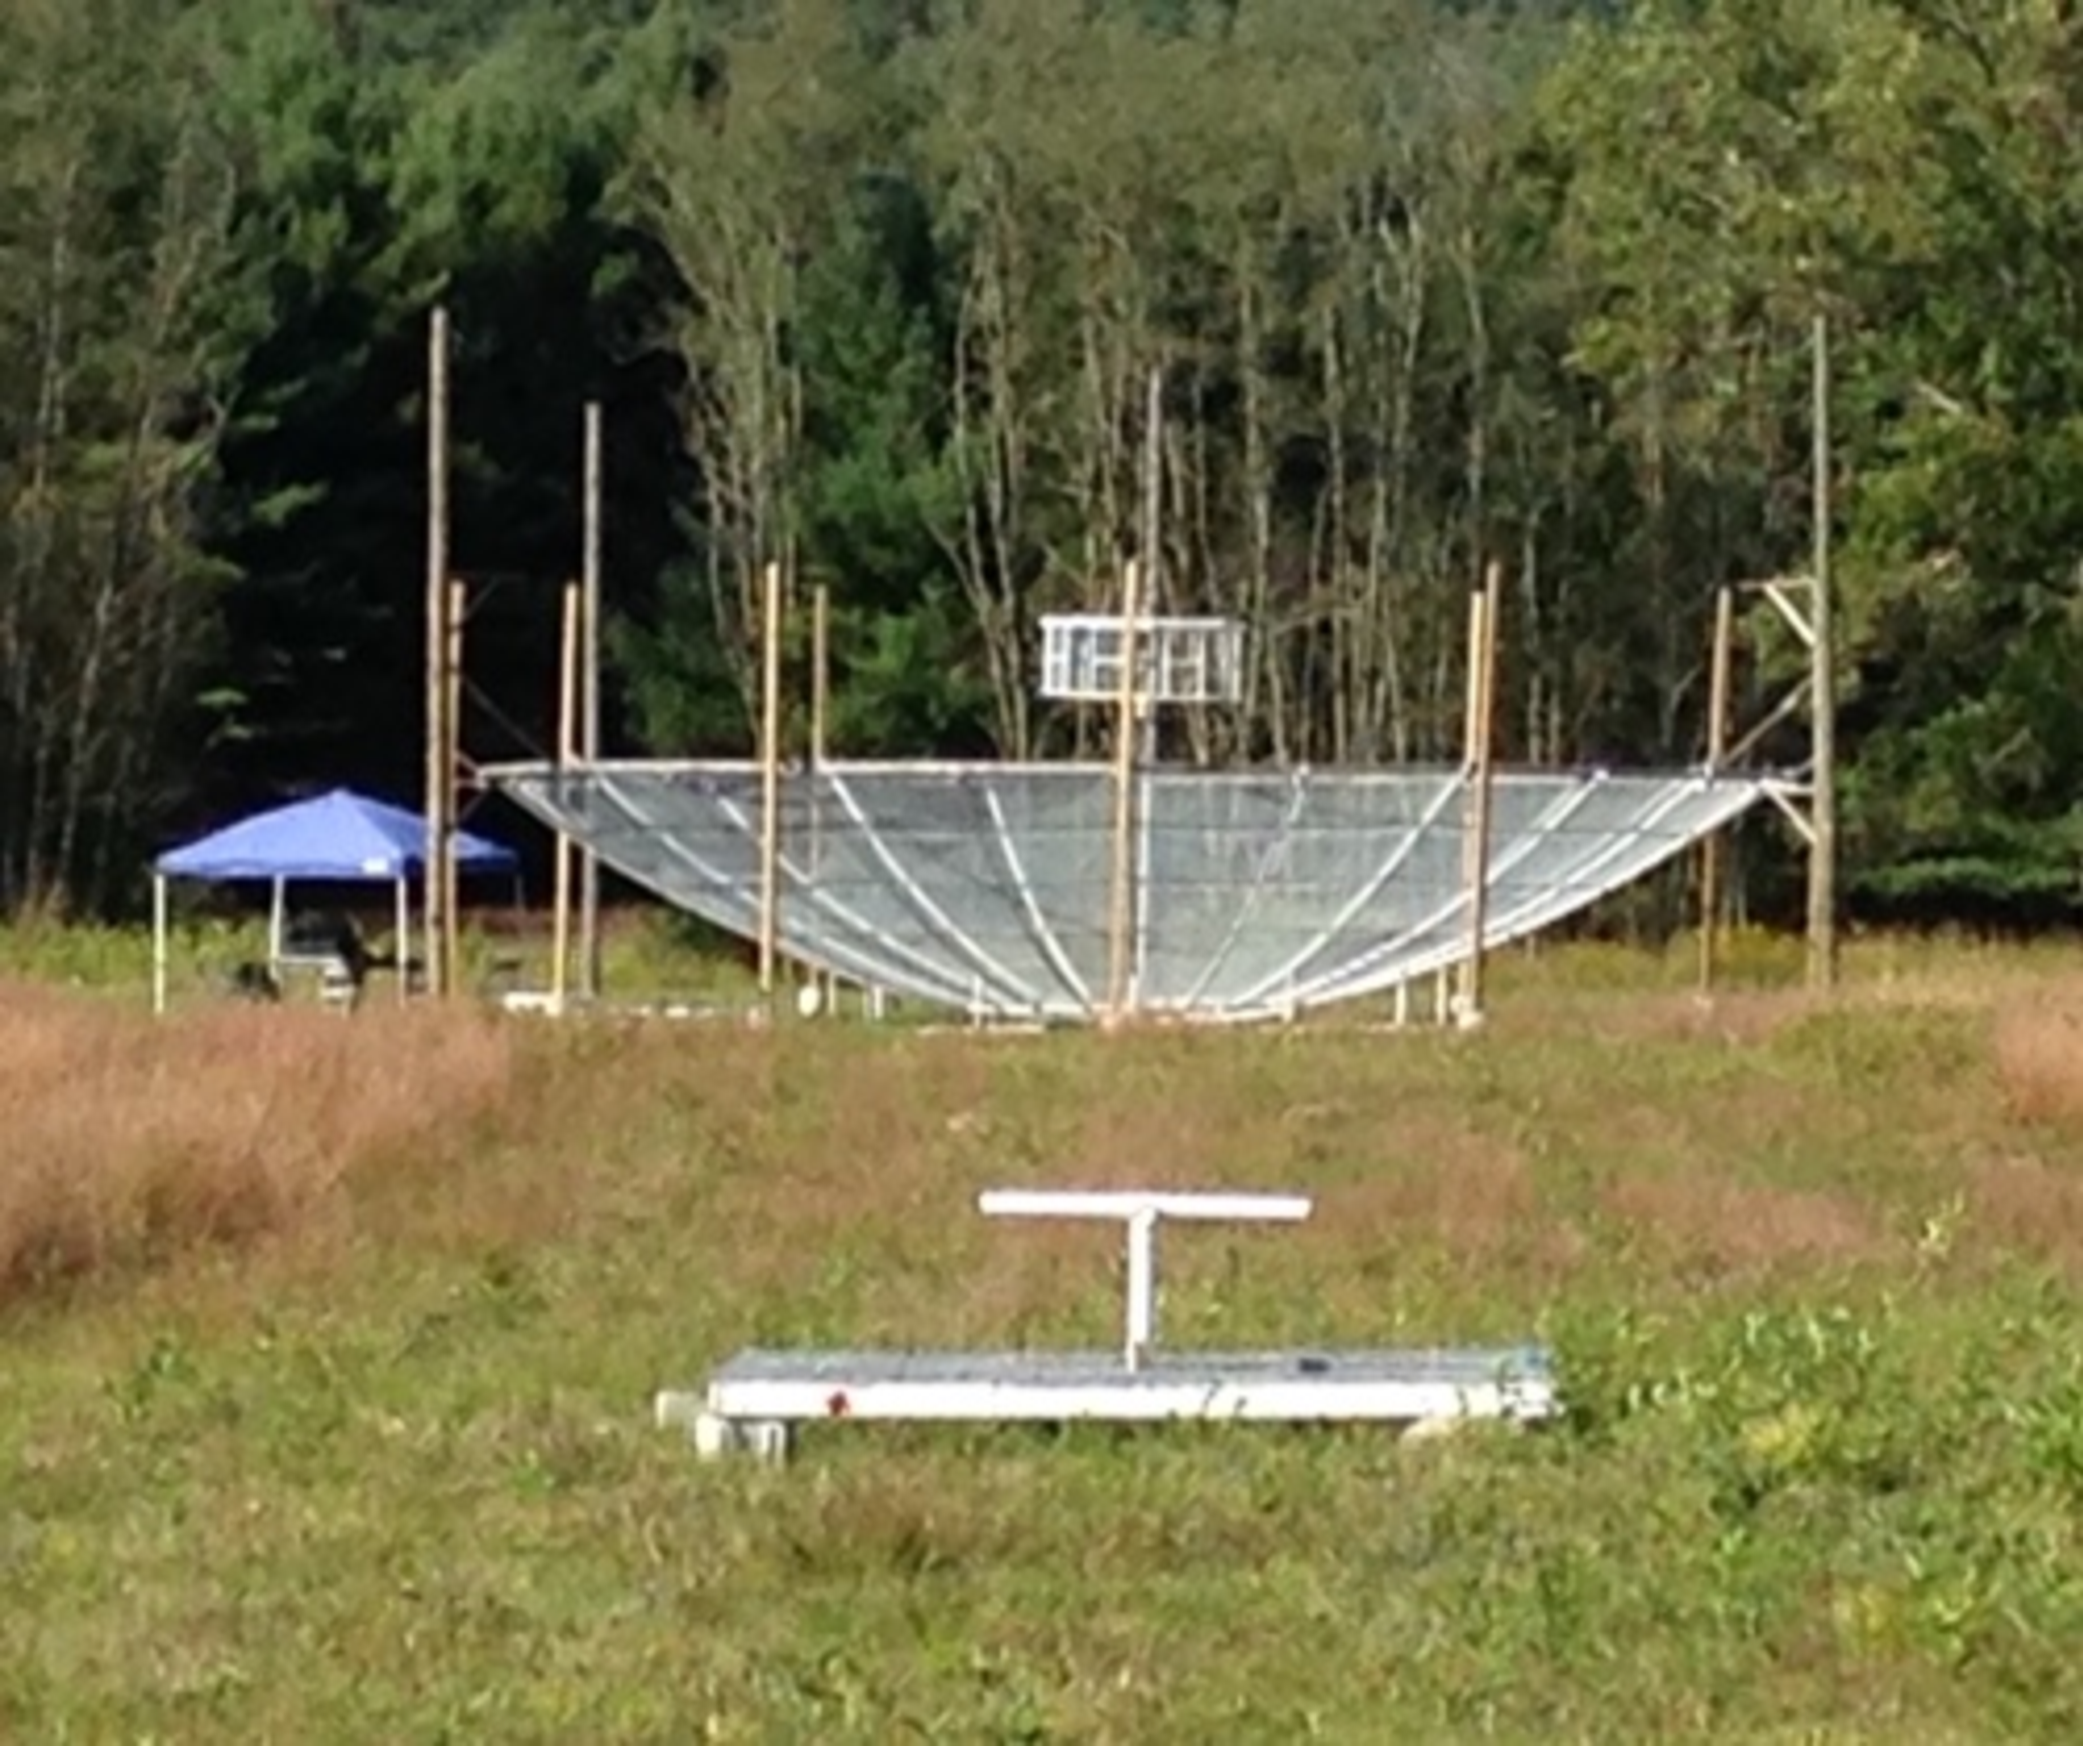
\includegraphics[width=3.4in]{chap3_hera_beammapping/ref_dipole_and_hera_dish.pdf}
\caption[The dish with its suspended feed is seen in the back of this image.]{The dish with its suspended feed is seen in the back, 50\,m north of one of the reference antennas used in the null experiment to study systematics. The experiment is conducted in Galford Meadow at NRAO--Green Bank.}
\label{fig:greenbankdishphoto}
\end{figure}

We use a simple dual-polarization dipole as our reference antenna. The dipole is constructed out of copper tubing covered by PVC for protection, mounted above a 2\,m $\times$ 2\,m ground plane. See \citet{neben15} for details. During the dish measurements the dipole is positioned 100\,m due south of the dish, though we experiment with other locations in order to characterize the environmental systematics of these measurements, as detailed in the next section. Figure \ref{fig:greenbankdishphoto} shows the dish with suspended feed 50\,m north of one of the reference antennas.

\subsection{Assessing Experimental Systematics}

\begin{figure*}[h]
\centering
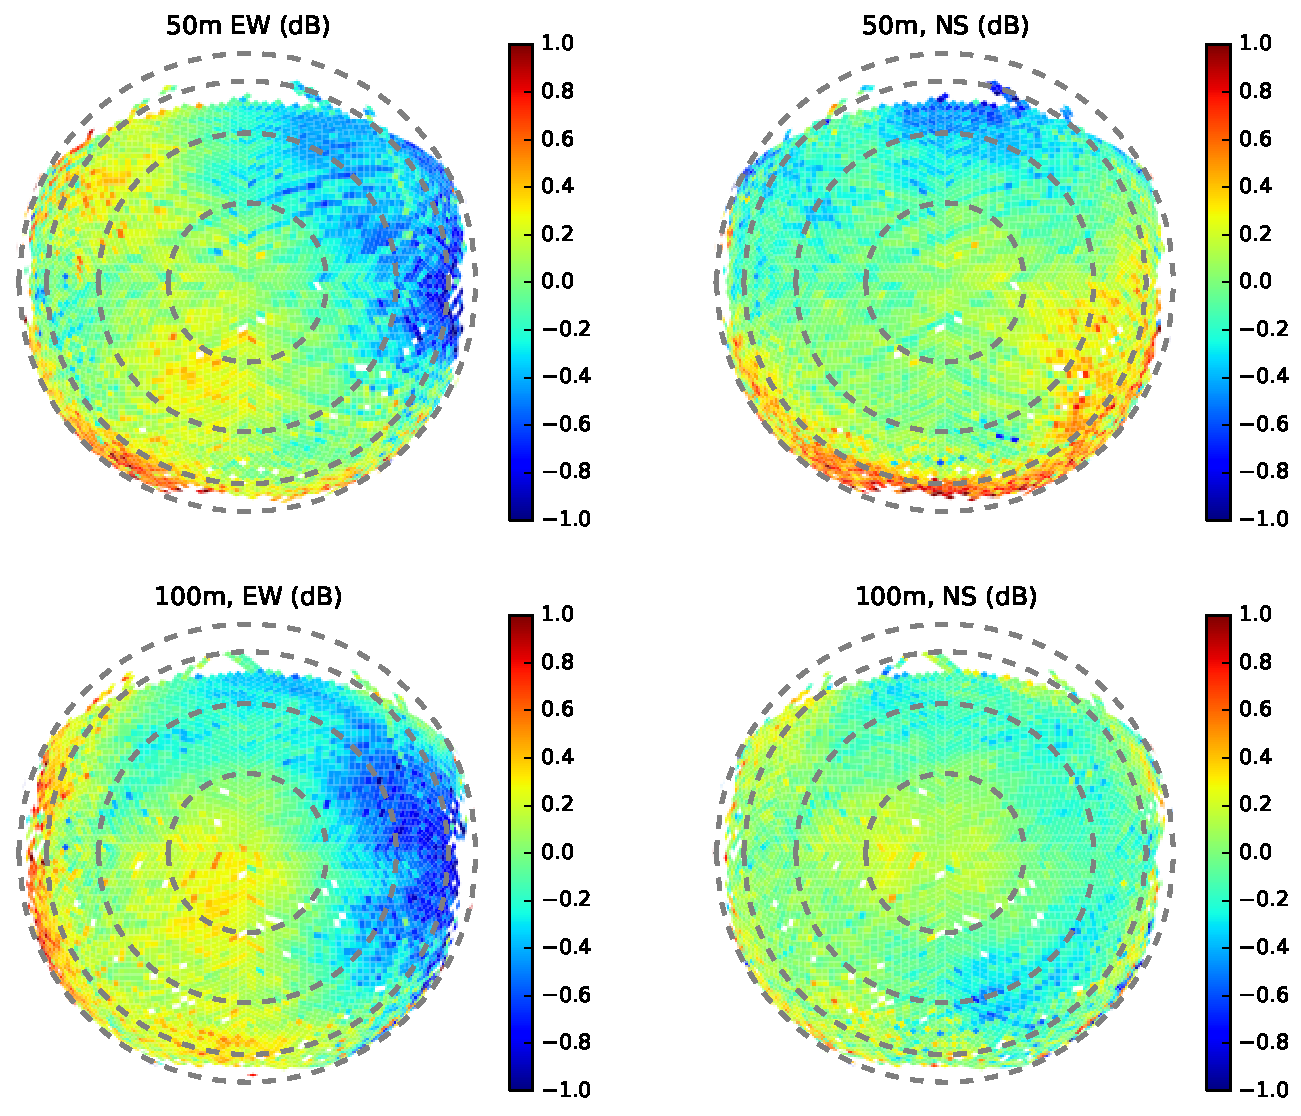
\includegraphics[width=6in]{chap3_hera_beammapping/null_expt_rel_beam_maps.pdf}
\caption[Null experiment results to characterize systematic errors.]{We characterize the accuracy of the beam measurement system through null experiments in which a second reference antenna is taken as the AUT and ratio of both reference antenna power patterns is measured for EW (left) and NS (right) polarizations. The reference antennas are separated by 50\,m from each other and from the HERA dish in the first experiment (top), and by 100\,m from each other and from the HERA dish in the second experiment (bottom).}
\label{fig:nullexptplots}
\end{figure*}

As in \citet{neben15}, we assess systematics using a ``null experiment'' in which we use a second reference dipole as the antenna-under-test (AUT). Taking the ratio of its measured power pattern with the model beam pattern amounts to a ratio of the raw power responses received by the two antennas as a function of satellite direction. This probes the level of environmental systematics (i.e., reflections and varying ground properties) and antenna fabrication imperfections which affect each antenna differently. This is not a probe of modeling imperfections common to both antennas, but we expect such errors to be subdominant as the physical properties of the antenna are easier to characterize, and thus simulate, than misalignments and local environmental effects. 

As we are not able to replace the HERA dish with a reference antenna, we run two null experiments with both reference dipoles deployed (1) 50\,m apart on a NS line, 50\,m south of the HERA dish; and (2) 100\,m apart on a NS line, 100\,m south of the HERA dish. Figure \ref{fig:nullexptplots} shows the results from these experiments in the form of the ratio of the power responses of the two antennas. We collected roughly 100 satellite passes. Systematics at the few percent level are observed within $20^\circ$ of zenith, and at the 10--20\% level farther out. The magnitude and angular distribution of these systematics changes modestly as the separation is changed, suggesting that the reference dipoles differ largely due to intrinsic differences, with some environmental variation. In any case, these fractional errors propagate directly into our measured dish power patterns.

\section{Dish Measurements}

\subsection{Power pattern measurements}
\label{sec:powerpatternmeasurements}

\begin{figure*}[t]
\centering
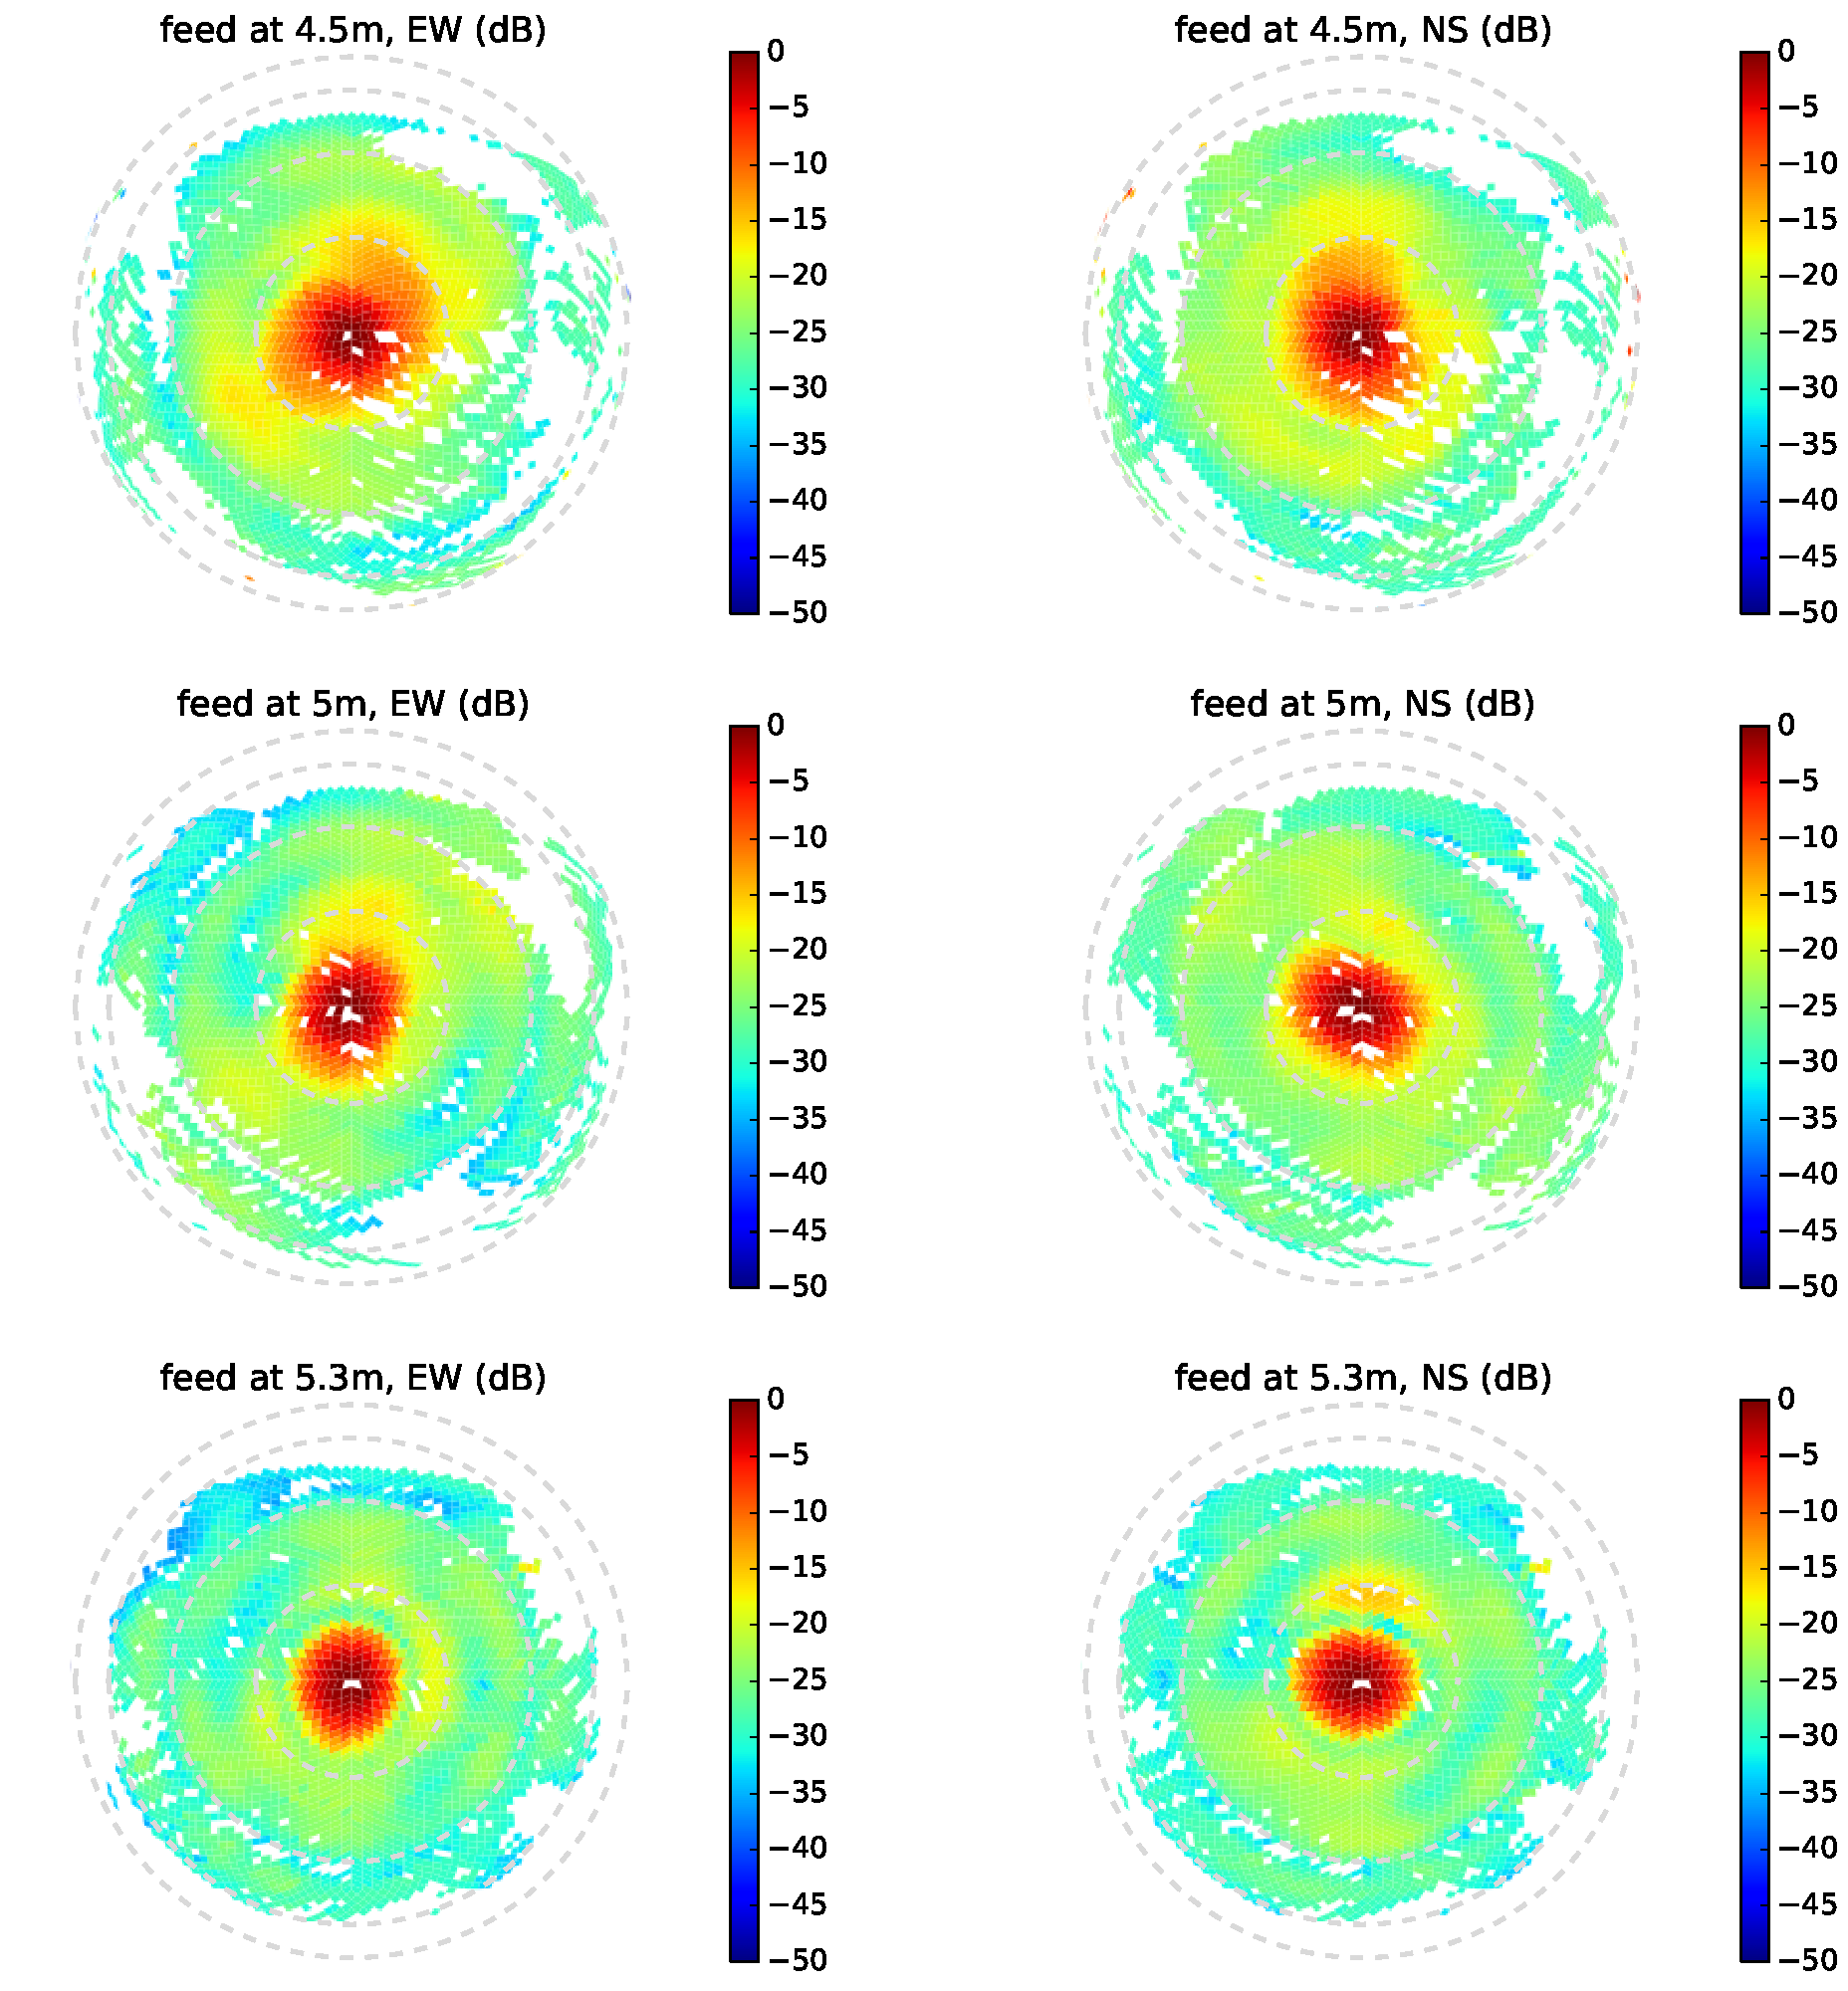
\includegraphics[width=6in]{chap3_hera_beammapping/measured_beams_and_models_maps.pdf}
\caption[Measured dish power patterns at three feed rigging heights.]{Measured dish power patterns at three feed rigging heights (Fig. \ref{fig:feeddiagram}) for the EW (left panel) and NS (right panel) instrumental polarizations. The sidelobes shrink and the main lobe narrows as the feed is raised, confirming that the best focus is close to $h_\text{rig}=5.3$\,m.}
\label{fig:measuredbeammaps}
\end{figure*}

\begin{figure*}[t]
\centering
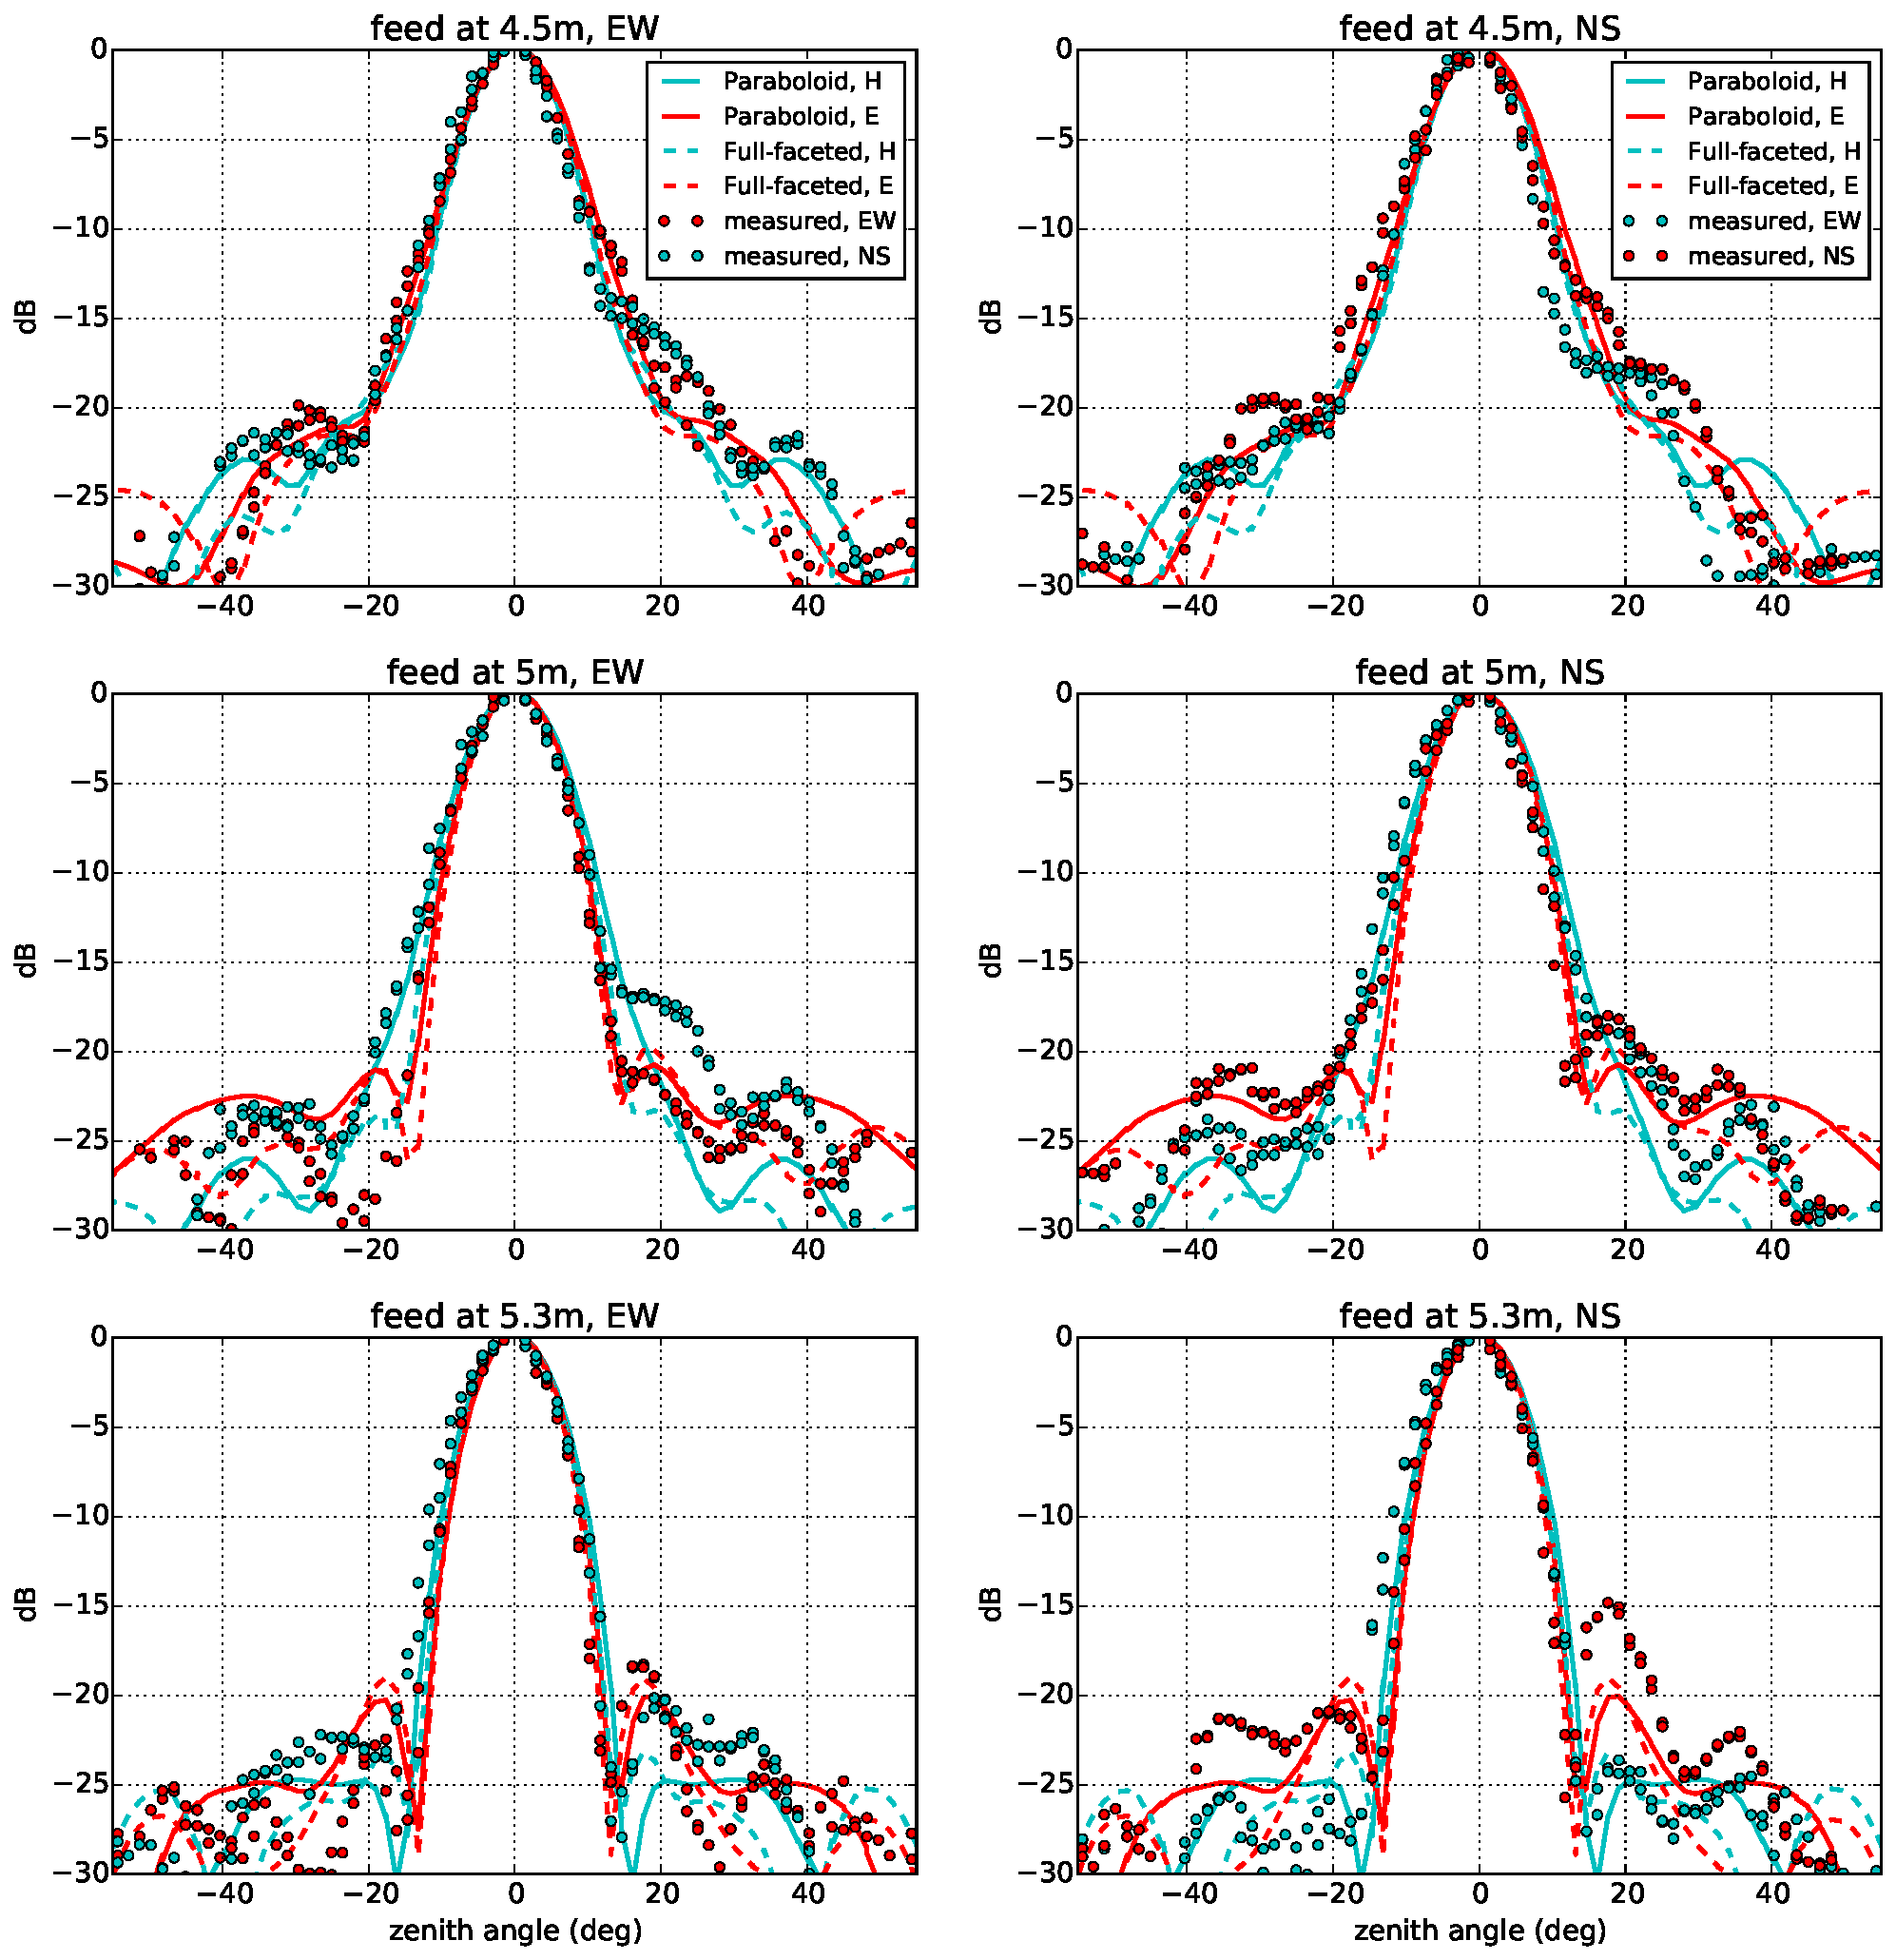
\includegraphics[width=6in]{chap3_hera_beammapping/measured_beams_and_models_slices.pdf}
\caption[Slices through the E (red) and H (cyan) planes through the measured dish power patterns (points) and numerical models (curves).]{Slices through the E (red) and H (cyan) planes through the measured dish power patterns (points) and numerical models (curves). The measured beams agree with both models in the main lobe out to zenith angles of 15--20$^\circ$ up to slight main lobe tilts, but begin to deviate in the sidelobes where the beam response is 25-30\,dB down from zenith. The measured beams typically differ more from both model beams than the models differ from each other, suggesting that real world effects are more significant that the slightly different assumptions used the two beam models. In particular, the most likely systematic is mis-centering of the feed over the dish (see Sec. \ref{sec:powerpatternmeasurements}).}
\label{fig:measuredbeamslices}
\end{figure*}

We make dish power pattern measurements at 137\,MHz as described in Sec. \ref{sec:orbcommreview} with feed rigging heights of 4.5\,m, 5.0\,m, and 5.3\,m above the dish surface (see Fig. \ref{fig:feeddiagram}). In each configuration we collect data for 2--4 days, obtaining roughly 200 satellite passes. We exclude times when the received power is within 20\,dB of the background level determined between passes, and then grid measured beam values into 1.8$^\circ$ HEALPix cells on the sky, rejecting outliers in the top or bottom 5\% in each cell as a final guard against rare satellite identification problems or ADC saturation issues.

Fig. \ref{fig:measuredbeammaps} shows the measured power patterns for these three feed heights for the EW (left panel) and the NS (right panel) feed polarizations. These maps are plotted in sine-projection with dashed circles marking zenith angles of $20^\circ$, $40^\circ$, $60^\circ$, and $80^\circ$. The sky coverage in these dish measurements extends out to typically zenith angles of $\theta\sim60^\circ$, beyond which the ORBCOMM flux is sufficiently attenuated relative to diffuse galactic emission that a power measurements is no longer a clean probe of the antenna gain in the direction of the satellite. At these largest measurable zenith angles the beam sidelobes are roughly -30\,dB down from the zenith boresight gain, and trending downward. 

The roughly $10^\circ$ full-width-at-half-max main lobe narrows slightly as the feed is raised from 4.5\,m to 5.3\,m, and the sidelobes shrink in size and amplitude, confirming that the best focus is closer to 5.3\,m. As discussed in Sec. \ref{sec:dishmodels}, the dish beam should be narrower in the E plane and wider in the H plane, with an overall 180$^\circ$ symmetry. Indeed, the observed main lobes of the EW (NS) beams are slightly wider in the NS (EW), especially in the 5.3\,m feed height beam as it is most in focus. We observe deviations from this symmetry in the sidelobes, which are very sensitive to slight dish/feed imperfections. 

Figure \ref{fig:measuredbeamslices} shows slices through the E and H planes of these power patterns along with the full-faceted and perfect paraboloid numerical models discussed earlier. As in the previous plot, the EW and NS beams are shown in the left and right panels, while the different feed heights are shown in the different rows. The data agree with both models to within 1\,dB in the main lobe, though in several cases appear slightly shifted so they are not quite centered on zenith. The data diverge further in the sidelobes at zenith angles of $20^\circ$ and larger. Here the evolution of the sidelobes as the feed is raised is again seen starkly, as is the fact that the main lobes are slightly wider along the H planes than along the E planes. We observe that both models agree with the measured beams in the main lobe but deviate from the data in different ways at the 1--5 dB level in the sidelobes. Neither model agrees consistently better with the data, suggesting that real-world imperfections of the HERA dish dominate over the slightly different modeling assumptions. 

We emphasize that the model deviations observed in the measured beams are real in that they are larger than the 0.5\,dB scale systematics observed in the null experiments (Fig. \ref{fig:nullexptplots}). Those experiments bound the impact of environmental reflections and reference dipole mismodeling to the 10\% level or smaller across the whole sky. The observed dish beam asymmetries, model deviations in sidelobes, and slight shifts of the main lobes all suggest feed centering errors. The feed is suspended by three ropes attached from the center of the feed back plane to three telephone poles spaced around the dish, and is raised by pulling all three ropes to a new length. Each time this is done the feed centering is slightly disturbed because all three ropes must be pulled to the exact same length to center the feed. Because all three ropes are attached to the same point on the feed, changing their lengths does not affect feed rotation or tilt. Thus if rotation or tilt errors, or dish surface imperfections, were significant, then the beam errors at different feed heights would look similar. The fact that the observed model deviations change with feed height suggests that feed centering errors are most significant. To mitigate all these feed positioning errors, the feeds in the full HERA array will be tied down to the dish surface at several points.

\subsection{Sensitivity}

We compute the effective collecting areas of these beam patterns by first interpolating over unmeasured cells and smoothly extrapolating the power pattern to the horizon. These operations produce a realistically smooth beam which reaches roughly -30\,dB at the horizon, as suggested by the numerical models. The collecting area $A$ is related to the beam power pattern $B(\theta,\phi)$ as
\begin{equation}
	A=\frac{\lambda^2 B(0,0)}{\int B(\theta,\phi)d\Omega}
\end{equation}

The collecting areas are shown in Table 1 along with the maximal collecting area achieved by the Airy pattern for a 14\,m dish. The measured collecting areas imply aperture efficiencies of 45--60\%. This is in line with expectations given the feed design which tapers the dipole beam towards the edges of the dish to reduce spillover into adjacent dishes. The mesh cylinder hanging from the feed back plane around the dipole also reduces the aperture efficiency slightly in order to make the feed beam more azimuthally symmetric. 

 \begin{table}[h]
 \caption[Collecting area of 137\,MHz HERA beams and resulting SNR predictions.]{ \label{table:collectingareatable}Collecting area (m$^2$) of measured 137\,MHz beams and corresponding power spectrum SNR for HERA-320 using either foreground avoidance or foreground subtraction.}
\begin{tabular}{| l | l | l |}
\hline
Beam & $A_\text{eff}$ (m$^2$) & SNR ($\sigma$)\\
&& (avoidance, subtraction)\\
\hline
  Airy pattern & 155 & 18.7, 90.8  \\
    Measured, feed at 5.3\,m & 93.0 & 12.7, 74.3 \\
    Measured, feed at 5\,m & 77.1 &  10.6, 67.9 \\
    Measured, feed at 4.5\,m & 68.5 &  10.0, 63.9 \\ 
  \hline
\end{tabular}
\end{table}

% To input these collecting areas into 21cmSense, we convert these measured dish collecting areas into effective dish diameters, which we input as the \texttt{dish\_size\_in\_lambda} parameter. 
We run 21cmSense\footnote{https://github.com/jpober/21cmSense} to compute the overall SNR of a power spectrum detection with one season (6 hours per night for 180 nights) of HERA-320 data. We use a fiducial Epoch of Reionization model generated with 21cmFast \citep{21cmfast}. This model assumes $\zeta=31.5$ for the ionizing efficiency, $T_\mathrm{vir}=1.5\times10^4$\,K for the minimum virial temperature of halos producing ionizing photons, and $R_\text{mfp}=30$\,Mpc for the mean free path of ionizing photons, and reaches 50\% ionization at $z \sim 9.5$ and complete ionization at $z \sim 7$, and is consistent with current observations \citep[e.g.][]{PoberNextGen}. 

We predict SNRs first for a foreground \textit{avoidance} approach where only modes outside of the wedge plus a buffer of $\Delta k_\parallel=0.15\,\mathrm{h}\,\mathrm{Mpc}^{-1}$ are used. These modes have frequency dependence larger than that of any smooth spectrum source on the sky, and this buffer size is chosen to exclude modes which leak out of the wedge due to beam frequency dependence. Due to imperfect impedance matching at the center of the 100-200\,MHz band, the $z\sim8.5$ band requires a slightly larger buffer, though our chosen buffer effectively avoids the leakage in other bands \citep{ewallwice16}. We also predict SNRs for a foreground \textit{subtraction} approach using all modes whose instrumental frequency dependence is larger than that of a source at the edge of the main lobe. 

The SNRs computed with the measured collecting areas are 10-13 with foreground avoidance compared with 19 for the Airy pattern. With foreground subtraction, the SNR falls from 90 with the Airy pattern to 60-75 with the measured collecting areas. In all cases this reduction is a loss of sensitivity, but a power spectrum detection is still always very significant at the 10$\sigma$ level or better.

\section{Foreground Delay Spectrum Simulations}
\label{sec:foregrounds}

We consider now the effects of the beam power pattern on the apparent frequency dependence of the foregrounds. \citet{nithya16} discuss the apparent frequency dependence of foregrounds in more detail as well as the contribution from the beam frequency dependence. We focus in this section on the uncertainties in these foreground power spectrum simulations due to beam modeling uncertainties, but first discuss these foreground simulations themselves and their dependence on observing conditions. 

We simulate foreground power spectra using different primary beam models at various local sidereal times (LSTs). We use frequency-independent model beams (evaluated at 137\,MHz) to isolate the interferometric foreground frequency dependence. The added frequency dependence of the changing overall gain and beam shape with frequency is addressed by the other papers in this series. Given that our measured dish power patterns agree well with both numerical models (full-faceted and perfect paraboloid) in the main lobe but deviate in the sidelobes, and that these models make somewhat different assumptions about the dish surface, we take them as a representative pair of possible dish models. We use the empirically best feed height of 5.3\,m. We also include the Airy pattern for comparison as in \citet{nithya15}. Beam models with weaker response near the horizon (such as the Airy pattern) downweight sources in this direction of high apparent frequency dependence. This reduces the magnitude of emission near the edge of the EOR window, reducing the risk it leaks inside. We use the per-baseline approach of \citet{parsons12a,parsons12b} by first simulating visibilities measured by specific baselines as a function of frequency, then computing the Fourier transform over frequency (delay transform), and lastly normalizing the result into a cosmological power spectrum following \citet{nithya15}. 

In detail, we simulate visibilities using the Precision Radio Interferometry Simulator\footnote{https://github.com/nithyanandan/PRISim} (PRISim) for each beam model at various LSTs, modeling the sky as the sum of the Global Sky Model \citep{gsm} and the NVSS \citep{nvss} and SUMSS \citep{sumss,sumss2} point source catalogs. We use a frequency spacing of 781\,kHz, sufficient to characterize delays within and just outside of the horizon limits on both baseline lengths considered, 14.6\,m and 43.8\,m. We use a total bandwidth of 100\,MHz (effectively reduced to 50\,MHz after applying the Blackman-Harris window) centered on 150\,MHz. This bandwidth is larger than the 10\,MHz thought to be safe from signal evolution with redshift, but is the bandwidth used in the wide band delay space foreground filter of \citet{parsons14,ali15}.

Figure \ref{fig:delayspec} (top panel) shows simulated foreground delay spectra at various LSTs using the full-faceted beam. As all these LSTs correspond to high galactic latitudes far from the galactic center, the total visibility power (the level of the zero delay mode) varies only by a factor of a few over these LSTs on both baseline lengths (14.6\,m (left panel), 43.8\,m (right panel)). However the positive delay horizon limit (corresponding to the western horizon) has a peak that varies by over 1.5 orders of magnitude on both baselines, demonstrating the stark difference in horizon brightening when the galaxy is just above versus just below the horizon. In this figure we perform the approximate conversion from delay $\tau$ to $k_\parallel$ at $z=8$, which we plot as a second $x$-axis at the top of the plot. 

\begin{figure*}[h]
\centering
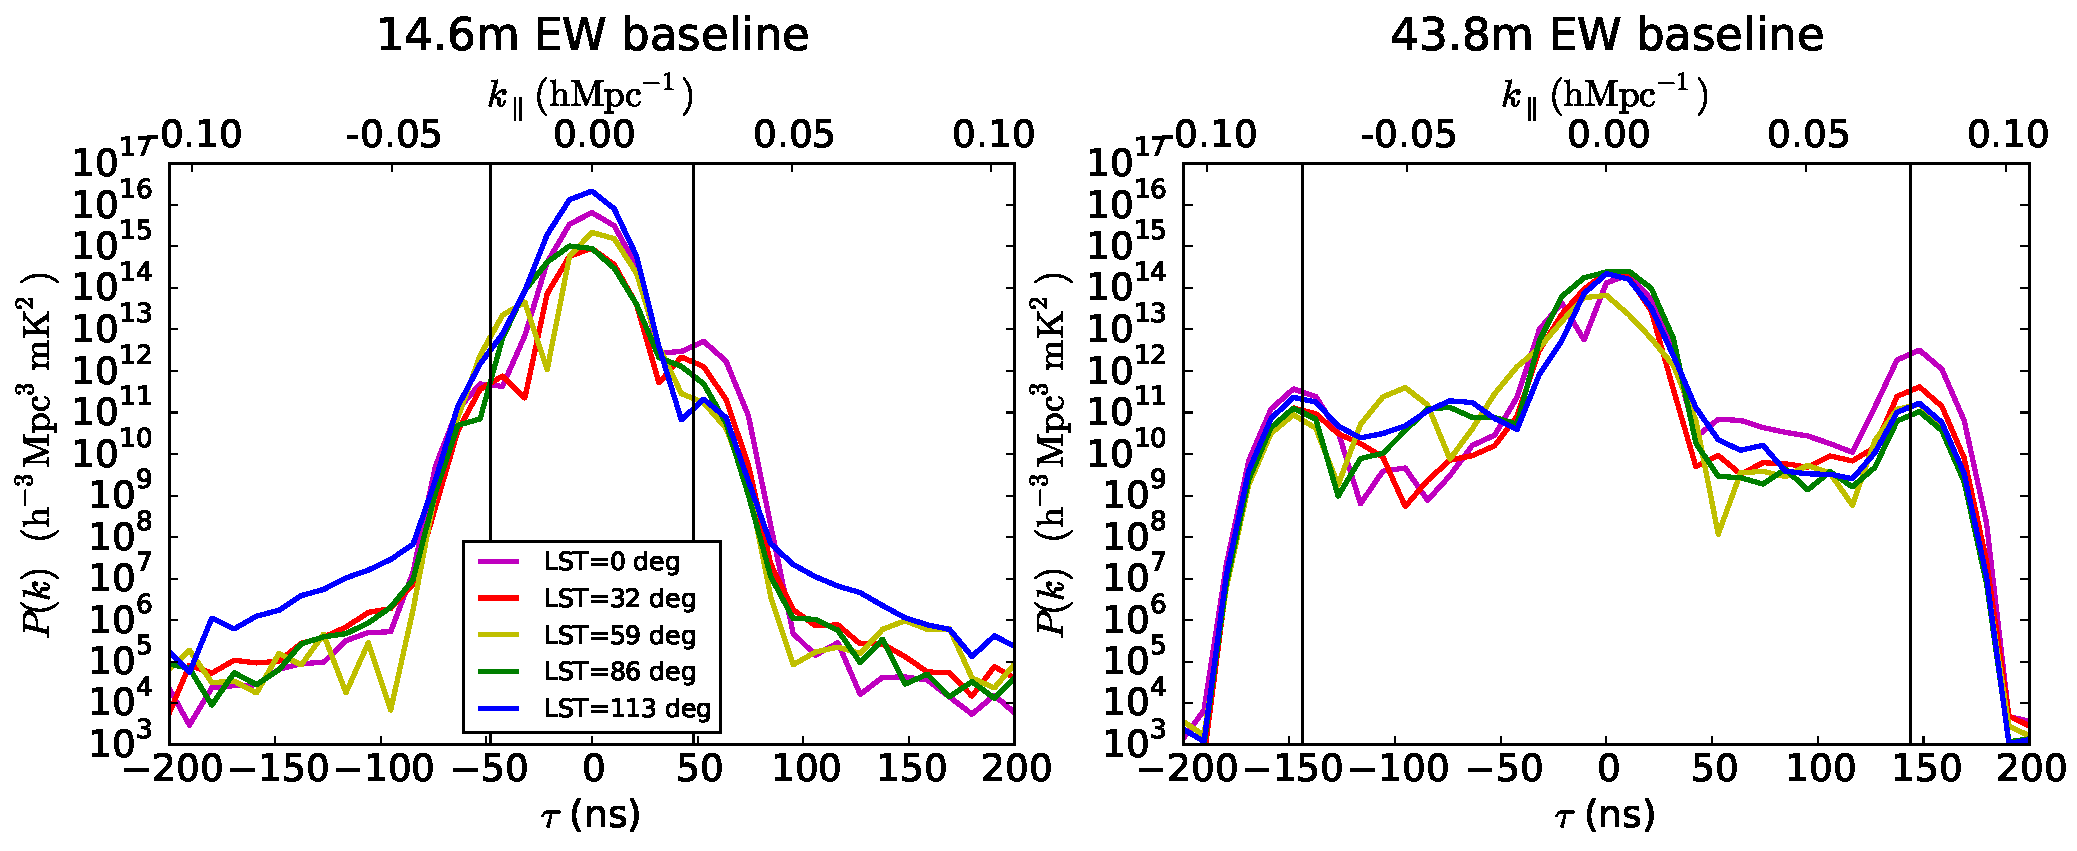
\includegraphics[width=6in]{chap3_hera_beammapping/nithya_fg_pspec_all_lst.pdf}
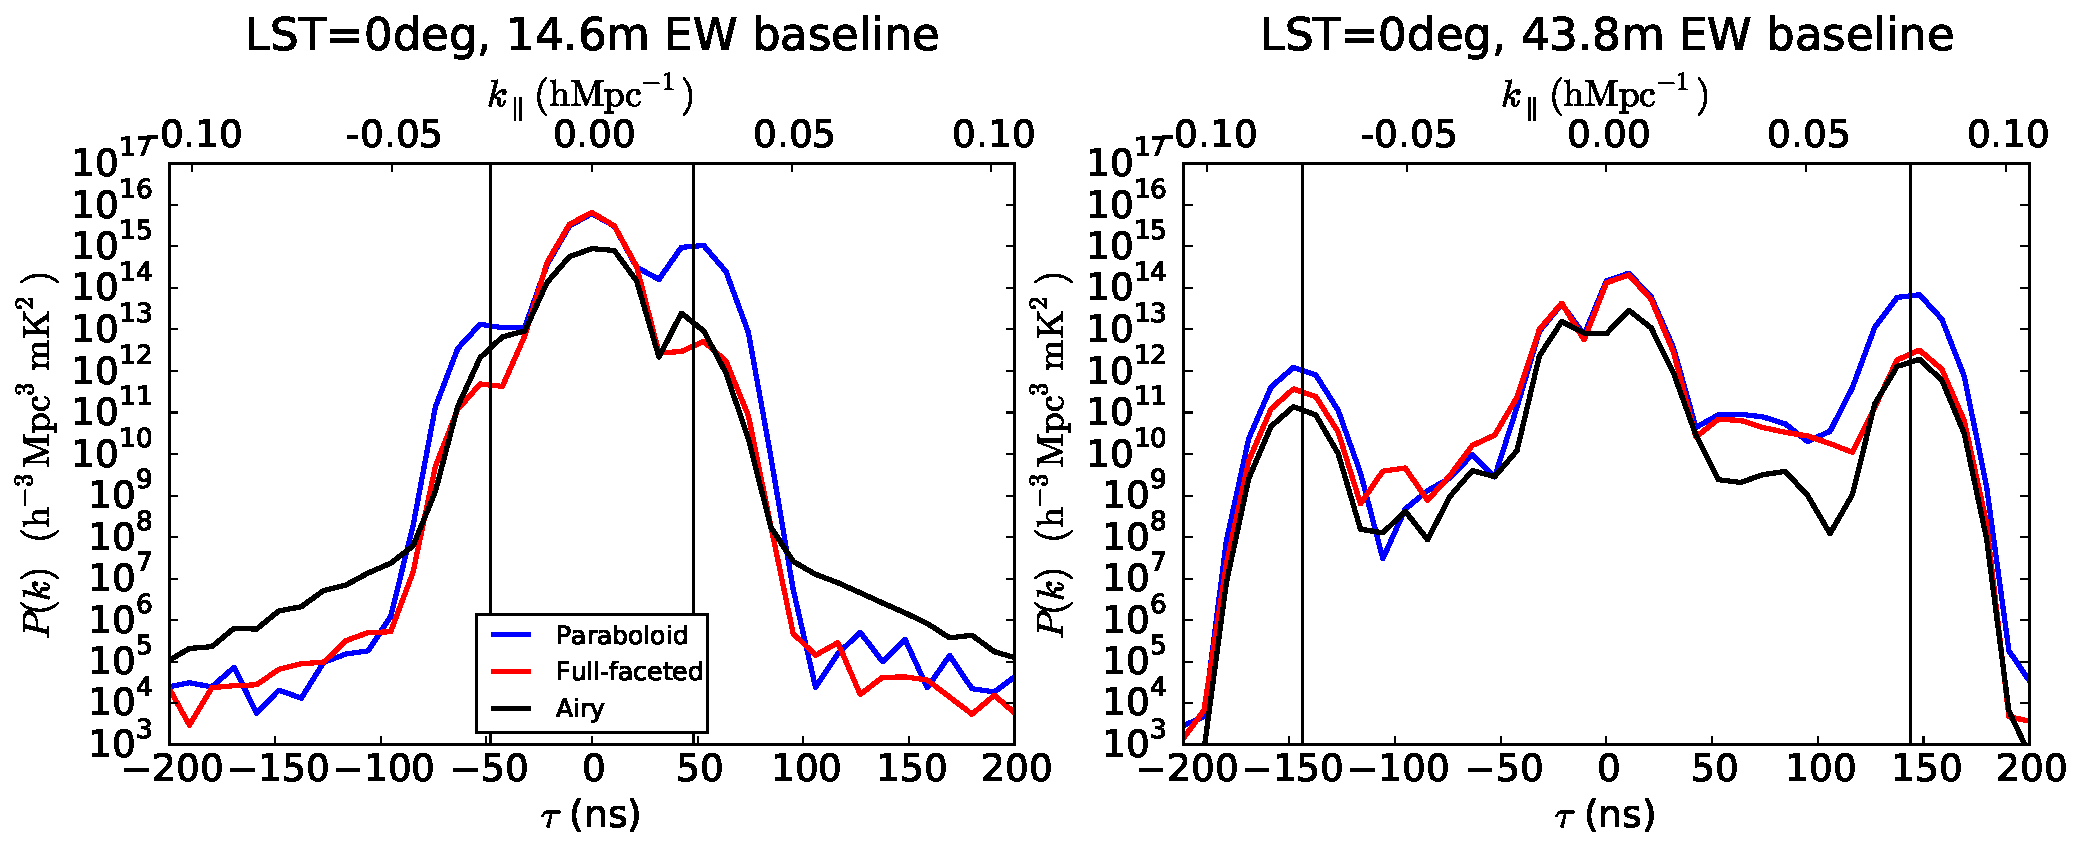
\includegraphics[width=6in]{chap3_hera_beammapping/nithya_fg_pspec_lst0deg.pdf}
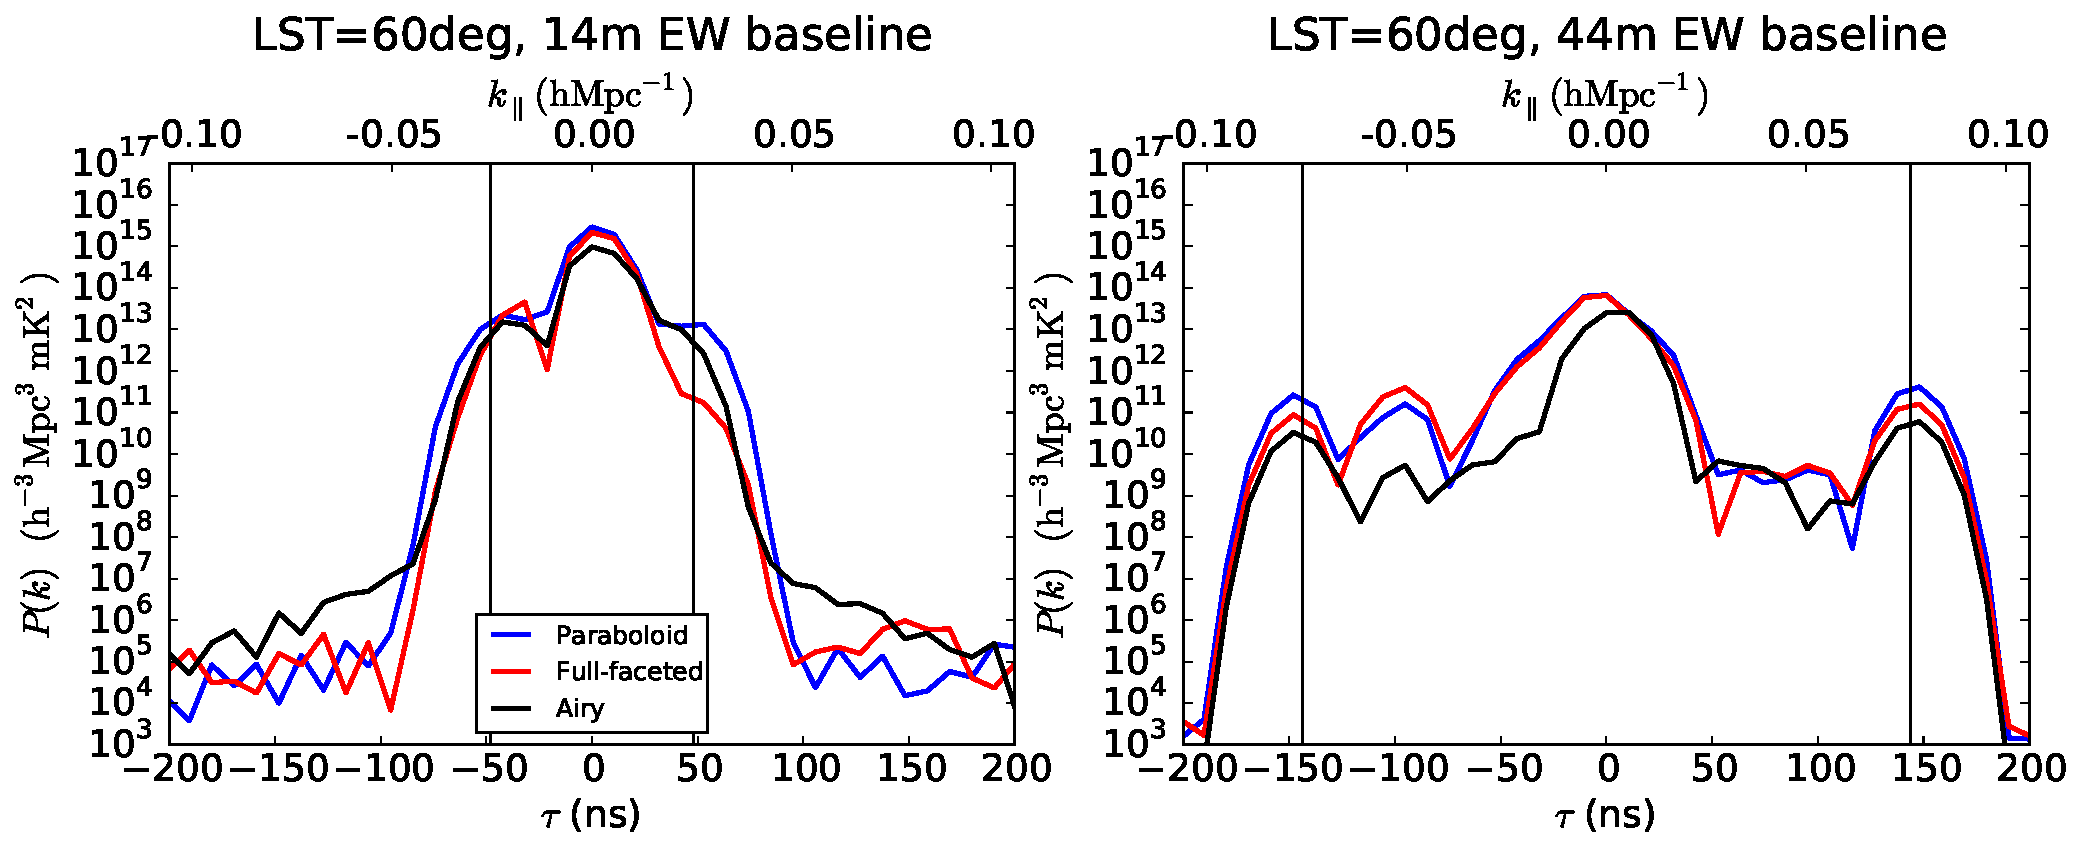
\includegraphics[width=6in]{chap3_hera_beammapping/nithya_fg_pspec_lst60deg.pdf}
\caption[We plot simulated foreground delay spectra using the full-faceted beam at various LSTs (top panel).]{We plot simulated foreground delay spectra using the full-faceted beam at various LSTs (top panel). The maximum horizon brightening at the positive horizon occurs close to 0$^\circ$ LST. At this LST, the simulated foreground delay spectra for the three beam models differ markedly near the positive horizon, plotted as a vertical line at the baseline's maximum delay. In contrast, when the horizon brightening effect is smaller at 60$^\circ$ LST (bottom panel), the foreground delay spectra from all three beams agree better.}
\label{fig:delayspec}
\end{figure*}

To characterize the effect of beam modeling uncertainties on this horizon brightening, we select two of these LSTs, one with maximal horizon brightening ($0^\circ$), and one with minimal horizon brightening ($60^\circ$). Figure \ref{fig:gsmplots} shows the sine-projected Global Sky Model at 150\,MHz, which dominates the horizon brightening effect, in local Azimuth/Elevation coordinates with units of Kelvin for both LSTs. These plots confirm that the large positive delay peak at the 0$^\circ$ LST is due to the center of the galaxy just above the western horizon. In contrast, several hours later, the galactic center is fully below the horizon, leaving only a slight brightening near the eastern horizon due to the weaker galactic anticenter. 

\begin{figure*}[t]
\centering
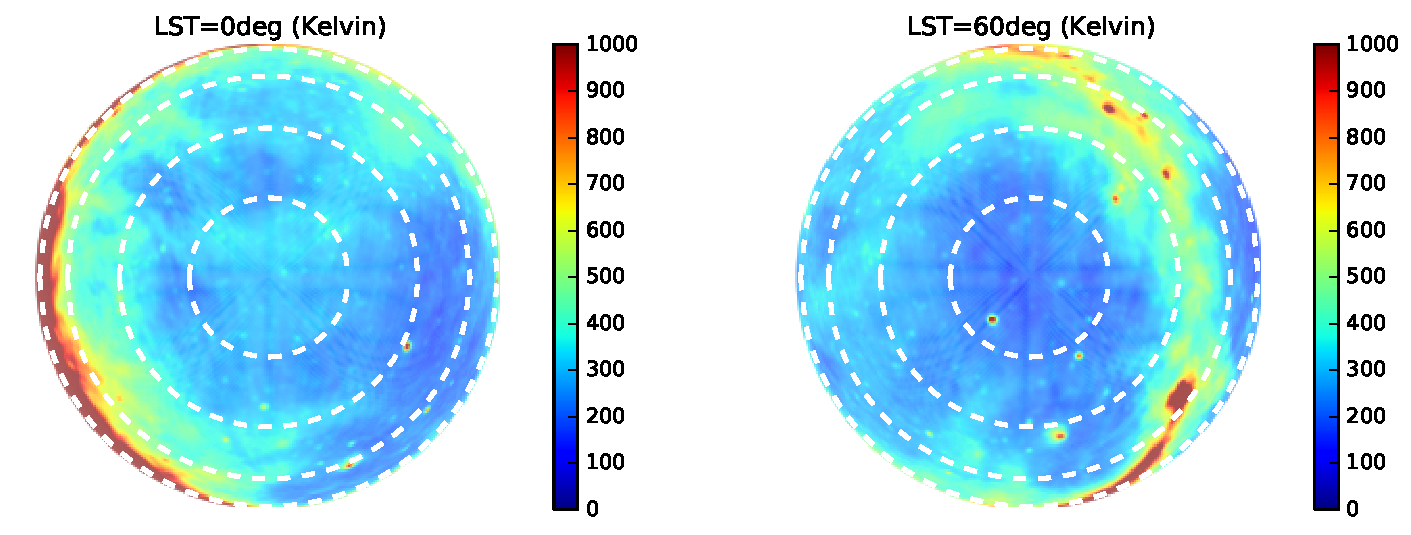
\includegraphics[width=6in]{chap3_hera_beammapping/gsm_kelvin_LST_2deg_and_62deg.pdf}
\caption[Global Sky Model.]{Global Sky Model \citep{gsm} in sine-projected horizontal coordinates at LST of 2$^\circ$ (left) and 60$^\circ$ right. The very bright emission from the center of the galaxy at the western horizon at 0$^\circ$ is seen in the delay spectra of EW baselines as a horizon brightening at negative delay.}
\label{fig:gsmplots}
\end{figure*}

How much do the predicted foreground power spectra differ between the three model dish power patterns? Figure \ref{fig:delayspec} (middle panel) shows the simulated delay spectra for all three beams at $0^\circ$ LST, when the horizon brightening is worst. Both numerical models agree out to delays of roughly 20\,ns on the 14.6\,m baseline and 50\,ns on the 43.8\,m baseline. These numbers suggest that the beams track each other fairly well out to roughly 25$^\circ$ from zenith, beyond which they diverge. This is roughly what is observed in Figure \ref{fig:measuredbeamslices}. At larger delays, especially near the positive delay horizon limit, all three model delay spectra diverge due to the significant edge brightening which effectively discriminates between these models. The perfect paraboloid and full-faceted beams reach roughly -32\,dB and -38\,dB at $80^\circ$ zenith angle (Figure \ref{fig:modelbeams}), consistent with the fact that the perfect paraboloid beam has a larger horizon brightening than the full-faceted beam. This is seen in the delay spectra for both baseline lengths, though the edge brightening is much clearer on the longer baseline where it less diluted by zero delay emission.  

In contrast, all three models agree better when there is little or no edge brightening as in Figure \ref{fig:delayspec} (bottom panel) where we plot the delay spectra for all three beams for 60$^\circ$ LST. There is still a modest flattening off near the horizon on the 14.6\,m baseline and a slight peak on the 43.8\,m baseline due to the large solid angle near the horizon. However as the near horizon emission at this LST is roughly the same temperature as emission from everywhere else on the sky, the difference between the three beam models is greatly reduced.

\section{Discussion}

Power spectrum analyses by first generation 21\,cm observatories are ongoing, but are contending with challenges ranging from calibration and foreground modeling to the analysis effort required to process thousands of hours of data. HERA draws on the most successful ideas from these first generation instruments, pursuing a compact and redundant array layout with large antenna elements. The hexagonal grid allows redundant calibration and coherent power spectrum integration, and the large 14\,m dish achieves sufficient sensitivity at a reasonable data processing and analysis cost. The papers in this series characterize HERA's 14\,m diameter dish element using reflectometry measurements and simulations, which probe its frequency response, as well as power pattern measurements probing its angular response. 

We have presented beam pattern measurements at 137\,MHz, and discussed their implications for 21\,cm power spectrum analyses in terms of sensitivity and foreground isolation. We begun with power pattern measurements made using the beam mapping system of \citet{neben15} which we deployed at the prototype three-element HERA array at the National Radio Astronomy Observatory--Green Bank. We measured the dish power pattern with the feed at different heights over the dish surface and found that the best focus is at a feed rigging height of 5.3\,m, though this may change for different feed designs being explored \citep{feedoptimizationmemo}. The measured beams probe nearly two thirds of the visible sky down to -30\,dB relative to boresight, and agree well with both models in the main lobe out to 10--20$^\circ$ from zenith. The measured beams roughly track the predicted sidelobe levels at 20--30\,dB below zenith, deviating at the 1--5\,dB level.

These deviations away from models and away from 180$^\circ$ azimuthal symmetry are larger than the $\pm0.5$\,dB systematics observed in our null experiments which probe the accuracy of our beam measurement system, suggesting they are genuine measurements of the in situ dish beam. The most likely culprit is feed mis-centering which shifts and distorts the main lobe sidelobes. In the full HERA array, the suspended feeds will be tied to the dish surface at several points to fine tune the feed centering and leveling, and mitigate wind buffeting. Characterizing the level of antenna-to-antenna beam variation in the full HERA array and its effects on power spectrum analyses, as \citet{neben16} do for the MWA, is left as future work.

We quantify HERA's sensitivity to the 21\,cm power spectrum given our beam measurements by first computing the collecting area of the measured beams at the different feed rigging heights, finding 93\,m$^2$ at the best focus, implying an aperture efficiency of 60\%. Feed optimization is ongoing, but the present feed sacrifices aperture efficiency in order to taper the dipole beam towards the edges of the dish and make the X and Y dipole beams as similar as possible using a cylinder hanging from the back plane. We convert our measured collecting areas into effective dish sizes, then use 21cmSense to predict the overall power spectrum SNR at $z\sim9.5$ with one season of HERA-320 data. We predict SNRs of 12.7 and 74.3 using foreground avoidance and subtraction approaches respectively, compared with SNRs of 18.7 and 90.8 using an ideal unobstructed 14\,m aperture (Airy pattern). Still, these sensitivities permit a very significant detection of the 21\,cm signal after a single observing season.

Beyond simple sensitivity considerations, though, the beam pattern affects science analyses by reweighting celestial emission in different regions of the sky, which are then imprinted with different frequency dependence by the interferometer. Longer baselines are more susceptible to this effect, giving rise to a ``wedge'' shaped region in 2D Fourier space. \citet{nithya15} has highlighted that the distribution of foregrounds \textit{within} the wedge is important as well. If the beam falloff is sufficiently shallow at low elevations, there is a relative brightening of emission from near the horizon in line with the baseline due in part to the large solid angle at low elevations. This produces a characteristic ``pitchfork'' shape in the delay spectrum of a single baseline, with a zero delay peak due to bright near-zenith emission surrounded by tines at the negative and positive horizon limits due to emission from the two horizon directions in line with the baseline. These horizon peaks are \textit{most} at risk of leaking foreground power into the EOR window given chromatic instrumental responses such as bandpass miscalibration, though techniques are being developed to suppress emission from near the horizon \citep{parsonsoptimalfringeratefiltering}.

We predict the magnitude of this effect for the HERA element and discuss the uncertainties in this estimate due to beam modeling uncertainty. As expected, we find that the level of horizon brightening is largest when the galaxy is just above the horizon, and lowest when it is well below. When this pitchfork effect is large, we find that the uncertainty in its predicted amplitude is also large, as seen in the differences between the delay spectra calculated using full-faceted and perfect paraboloid beam models. When the effect is small, the two beam models produce much more similar results, highlighting the delay spectrum as an exquisite probe of the difficult-to-measure beam response at very low elevations. Of course the delay spectrum provides only an integrated measure of the beam, but some information can still be extracted. By forward modeling foreground delay spectra using different MWA primary beam models, for instance, it was observed that the MWA bowtie dipoles are better modeled as isotropic radiators than hertzian dipoles at these low elevations (N. Thyagarajan, private communication). Direct measurements using transmitter-equipped drones would be ideal and their development is ongoing \citep{drone1,drone2}.

As discussed by the other papers in this series \citep{ewallwice16,patra16,nithya16}, the frequency dependence of both the beam's angular response and its overall gain widen the delay kernel of a source, leaking power into the EOR window out to $k_\parallel\approx$0.15h\,Mpc$^{-1}$ over much of the 100-200MHz band. This leakage falls within the wedge buffer used in a fiducial foreground avoidance analysis, so our SNR projections take into account the sensitivity reduction due to beam chromaticity. These sensitivities can be improved using new techniques such as foreground covariance downweighting and fringe rate filtering \citep{ali15,parsonsoptimalfringeratefiltering}, which mitigate foreground leakage into the EOR window, thereby permitting a smaller buffer. Using only these previously demonstrated techniques, we project a $13\sigma$ detection of the EOR power spectrum with a single observing season which would provide begin to probe reionization models in detail and shed light on our cosmic dawn. 


\section*{Acknowledgements}
We thank Jonathan Pober, Gianni Bernardi, and Eloy de Lera Acedo for helpful comments on our manuscript. This work was supported by NSF grant AST-1440343, the Marble Astrophysics Fund, and the MIT School of Science. ARP acknowledges support from NSF CAREER award 1352519. AEW acknowledges support from an NSF Graduate Research Fellowship under Grant No. 1122374. DJC acknowledges support from NSF grant AST-1401708.

%Results that might change:
\newcommand{\modelResidualCorr}{0.116}
\newcommand{\limitDeltaSq}{3.7\times 10^4}
\newcommand{\limitk}{0.18}
\newcommand{\limitz}{6.8}
\newcommand{\wedgeBuffer}{0.02}

\newcommand{\BigO}[1]{\mathcal{O}(#1)}
\newcommand{\F}{\mathbf{F}}
\newcommand{\M}{\mathbf{M}}
\newcommand{\CC}{\mathbf{C}}
\newcommand{\beq}{\begin{equation}}
\newcommand{\eeq}{\end{equation}}
\newcommand{\Sig}{\mathbf{S}}
\newcommand{\Eye}{\mathbf{I}}
\newcommand{\x}{\mathbf{x}}
\newcommand{\kvec}{\mathbf{k}}
\newcommand{\N}{\mathbf{N}}
\newcommand{\n}{\mathbf{n}}
\newcommand{\m}{\mathbf{m}}
\newcommand{\mean}{\boldsymbol\mu}
\newcommand{\base}{\mathbf{b}}
\newcommand{\thvec}{\bm{\theta}}
\newcommand{\A}{\mathbf{A}}
\newcommand{\p}{\mathbf{p}}
\newcommand{\q}{\mathbf{q}}
\newcommand{\Proj}{\mathbf{\Pi}}
\newcommand{\PSF}{\mathbf{P}} 
\newcommand{\K}{\mathbf{K}}
\newcommand{\y}{\mathbf{y}}
\newcommand{\J}{\mathbf{J}}
\newcommand{\D}{\mathbf{D}}
\newcommand{\T}{\mathbf{T}}
\newcommand{\W}{\mathbf{W}}
\newcommand{\Q}{\mathbf{Q}}
\newcommand{\E}{\mathbf{E}}
\newcommand{\trans}{\mathsf{T}}
\newcommand{\rhat}{\hat{\mathbf{r}}}
\newcommand{\xhat}{\widehat{\x}}
\newcommand{\CHat}{\widehat{\CC}}

\chapter{New Power Spectrum Limits from Early MWA 128-Tile Data using Empirical Covariance Modeling}

The content of this chapter was originally published as Dillon, J.S., Neben, A.R. et al., \textit{Empirical covariance modeling for 21 cm power spectrum estimation: A method demonstration and new limits from early Murchison Widefield Array 128-tile data.}, Physical Review D, 91(12):123011, 2015.\\

The separation of the faint cosmological background signal from bright astrophysical foregrounds remains one of the most daunting challenges of mapping the high-redshift intergalactic medium with the redshifted 21\,cm line of neutral hydrogen. Advances in mapping and modeling of diffuse and point source foregrounds have improved subtraction accuracy, but no subtraction scheme is perfect.  Precisely quantifying the errors and error correlations due to missubtracted foregrounds allows for both the rigorous analysis of the 21\,cm power spectrum and for the maximal isolation of the ``EoR window'' from foreground contamination. We present a method to infer the covariance of foreground residuals from the data itself in contrast to previous attempts at \textit{a priori} modeling. We demonstrate our method by setting limits on the power spectrum using a 3\,h integration from the 128-tile Murchison Widefield Array. Observing between 167 and 198\,MHz, we find at 95\% confidence a best limit of $\Delta^2(k) < \limitDeltaSq$\,mK$^2$ at comoving scale $k = \limitk$\,$h$\,Mpc$^{-1}$ and at $z = \limitz$, consistent with existing limits.


\section{Introduction} \label{sec:intro}

Tomographic mapping of neutral hydrogen using its 21\,cm hyperfine transition has the potential to directly probe the density, temperature, and ionization of the intergalactic medium (IGM), from redshift 50 (and possibly earlier) through the end of reionization at $z\sim 6$. This unprecedented view of the so-called ``cosmic dawn'' can tightly constrain models of the first stars and galaxies \cite{FurlanettoReview, miguelreview, PritchardLoebReview, aviBook} and eventually yield an order of magnitude more precise test of the standard cosmological model ($\Lambda$CDM) than current probes \cite{mao08}. 

Over the past few years, first generation instruments have made considerable progress toward the detection of the power spectrum of the 21\,cm emission during the epoch of reionization (EoR). Telescopes such as the Low Frequency Array (LOFAR \cite{LOFARinstrument}), the Donald C. Backer Precision Array for Probing the Epoch of Reionization (PAPER \cite{parsons14}), the Giant Metrewave Radio Telescope (GMRT \cite{gmrtsignalloss}), and the Murchison Widefield Array (MWA \cite{lonsdale09,tingay13,mwascience}) are now operating, and have begun to set limits on the power spectrum. GMRT set some of the earliest limits \cite{gmrtsignalloss} and both PAPER \cite{DannyMultiRedshift} and the MWA \cite{X13} have presented upper limits across multiple redshifts using small prototype arrays. PAPER has translated its results into a constraint on the heating of the IGM by the first generation of x-ray binaries and miniquasars \cite{parsons14} and has placed the tightest constraints so far on the power spectrum \cite{ali15} and the thermal history of the IGM \cite{PoberPAPER64Heating}.

Despite recent advances, considerable analysis challenges remain. Extracting the subtle cosmological signal from the noise is expected to require thousand hour observations across a range of redshifts \citep{MiguelNoise,Judd06,LidzRiseFall,LOFAR2,AaronSensitivity,nithya13}. Even more daunting is the fact that the 21\,cm signal is probably at least 4 orders of magnitude dimmer than the astrophysical foregrounds---due to synchrotron radiation from both our Galaxy and from other galaxies \citep{gsm,Jelic08,BernardiForegrounds,pober13,InitialLOFAR1,InitialLOFAR2}. 

Recently, simulations and analytical calculations have established the existence of a region in cylindrical Fourier space---in which three-dimensional (3D) Fourier modes $\vec{k}$ are binned into $k_\|$ modes along the line of sight and  $k_\perp$ modes perpendicular to it---called the ``EoR window'' that should be fairly free of foreground contamination \cite{Dattapowerspec,AaronDelay,VedanthamWedge,MoralesPSShapes,Hazelton2013,CathWedge,nithya13,AdrianWedge1,AdrianWedge2}. Observations of the EoR window confirm that it is largely foreground-free \cite{pober13,X13} up to the sensitivity limits of current experiments. The boundary of the EoR window is determined by the volume and resolution of the observation, the intrinsic spectral structure of the foregrounds, and the so-called ``wedge.'' 

Physically, the wedge arises from the frequency dependence of the point spread function (PSF) of any interferometer, which can create spectral structure from spectrally smooth foregrounds in our 3D maps (see \cite{AdrianWedge1} for a rigorous derivation). Fortunately, in $k_\|$-$k_\perp$ space, instrumental chromaticity from flat-spectrum sources is restricted to the region below 
\beq  
k_\| = \theta_0 \frac{ D_M(z) E(z)}{D_H (1+z)} k_\perp, \label{eq:wedge}
\eeq
where $D_H \equiv c/H_0$, $E(z) \equiv \sqrt{\Omega_m(1+z)^3+\Omega_\Lambda}$, and $D_m(z) \equiv \int_0^z \mathrm{d}z'/E(z')$ with cosmological parameters from \cite{planck16}. The size of the region is determined by $\theta_0$, the angle from zenith beyond which foregrounds do not significantly contribute. While most of the foreground emission we observe should appear inside the main lobe of the primary beam, foreground contamination from sources in the sidelobes are also significant compared to the signal \cite{pober16,nithya15,nithya15b}. A conservative choice of $\theta_0$ is therefore $\pi/2$, which reflects the fact that the maximum possible delay a baseline can measure corresponds to a source at the horizon \cite{AaronDelay}. Still, this foreground isolation is not foolproof and can be easily corrupted by miscalibration and imperfect data reduction. Further, slowly varying spectral modes just outside the wedge are also affected when the foreground residuals have spectral structure beyond that imprinted by the chromaticity of the interferometer.

To confidently detect the 21\,cm EoR power spectrum, we need rigorous statistical techniques that incorporate models of the cosmological signal, the foregrounds, the instrument, the instrumental noise, and the exact mapmaking procedure. With this information, one may use estimators that preserve as much cosmological information as possible and thoroughly propagate errors due to noise and foregrounds through the analysis pipeline.

The development of such statistical techniques has progressed rapidly over the past few years. The quadratic estimator formalism was adapted \cite{LT11} from previous work on the cosmic microwave background \cite{Maxpowerspeclossless} and galaxy surveys \cite{Maxgalaxysurvey1}. It was accelerated to meet the data volume challenges of 21\,cm tomography \cite{DillonFast} and refined to overcome some of the difficulties of working with real data \cite{X13}.  Further, recent work has shown how to rigorously incorporate the interferometric effects that create the wedge \cite{AdrianWedge1,AdrianWedge2,dillonmapmaking}, though they rely on precision instrument modeling, including exact per-frequency and per-antenna primary beams and complex gains. A similar technique designed for drift-scanning telescopes using spherical harmonic modes was developed in \cite{Richard,shaw15}, which also demonstrated the need for a precise understanding of one's instrument.

However, at this early stage in the development of 21\,cm cosmology, precision instrument characterization remains an active area of research \cite{sutinjo2014,neben15,NewburghCHIMECal,pober12}. We thus pursue a more cautious approach to foreground modeling that reflects our incomplete knowledge of the instrument by modeling the residual foreground covariance from the data itself. As we will show, this mitigates systematics such as calibration errors that would otherwise impart spectral structure onto the foregrounds, corrupting the EoR window. While not a fully Bayesian approach like those of \cite{SutterBayesianImaging} and \cite{GibbsPSE}, our technique discovers both the statistics of the foregrounds and the power spectrum from the data. Our foreground models are subject to certain prior assumptions but are allowed to be data motivated in a restricted space. However, by working in the context of the quadratic estimator formalism, we can benefit from the computational speedups of \cite{DillonFast}. This work is meant to build on those techniques and make them more easily applied to real and imperfect data.

This paper is organized into two main parts. In Section \ref{sec:methods} we discuss the problem of covariance modeling in the context of power spectrum estimation and present a method for the empirical estimation of that foreground model, using MWA data to illustrate the procedure. Then, in Section \ref{sec:results}, we explain how these data were taken and reduced into maps and present the results of our power spectrum estimation procedure on a few hours of MWA observation, including limits on the 21\,cm power spectrum.

%%%%%%%%%%%%%%%%%%%%%%%%%%%%%%%%%%%%%%%%%%%%%%%%%%%%%%%%%%%%%%%%%%%%%%%%%%

\section{Empirical Covariance Modeling} \label{sec:methods}

Before presenting our method of empirically modeling the statistics of residual foregrounds in our maps, we need to review the importance of these covariances to power spectrum estimation. We begin in Section \ref{sec:review} with a brief review of the quadratic estimator formalism for optimal power spectrum estimation and rigorous error quantification. We then discuss in Section \ref{sec:CovTheory} the problem of covariance modeling in greater detail, highlighting exactly which unknowns we are trying to model with the data. Next we present in Section \ref{sec:empirical} our empirical method of estimating the covariance of foreground residuals, illustrated with an application to MWA data. Lastly, we review in Section \ref{sec:caveats} the assumptions and caveats that we make or inherit from previous power spectrum estimation work.

%%%%%%%%%%%%%%%%%%%%%%%%%%%%%%%%%%%%%%%%%%%%%%%%%%%%%%%%%%%%%%%%%%%%%%%%%%

\subsection{Quadratic Power Spectrum Estimator Review}\label{sec:review}

The fundamental goal of power spectrum estimation is to reduce the volume of data by exploiting statistical symmetries while retaining as much information as possible about the cosmological power spectrum \cite{Maxpowerspeclossless}. We seek to estimate a set of band powers $\p$ using the approximation that
\beq
P(\kvec) \approx \sum_\alpha p_\alpha \chi_\alpha (\kvec),
\eeq
where $P(\kvec)$ is the power spectrum as a function of wave vector $\kvec$ and $\chi_\alpha$ is an indicator function that equals 1 wherever we are approximating $P(\kvec)$ by $p_\alpha$ and vanishes elsewhere.

Following \cite{LT11,DillonFast,X13}, we estimate power spectra from a ``data cube''---a set of sky maps of brightness temperature at many closely spaced frequencies---which we represent as a single vector $\xhat$ whose index iterates over both position and frequency. From $\xhat$, we estimate each band power as
\beq
\widehat{p}_\alpha = \frac{1}{2}M_{\alpha\beta} \left(\xhat_1 - \mean\right)^\trans \CC^{-1} \mathbf{C},_\beta \CC^{-1} \left(\xhat_2 -\mean\right) - b_\alpha. \label{eq:QuadEst}
\eeq
Here $\mean = \langle \xhat \rangle$, the ensemble average of our map over many different realizations of the observation, and $\CC$ is the covariance of our map,
\beq
\CC = \langle \xhat \xhat^\trans \rangle - \langle \xhat \rangle  \langle \xhat \rangle^\trans.
\eeq 
$\mathbf{C},_\beta$ is a matrix that encodes the response of the covariance to changes in the true, underlying band powers; roughly speaking, it performs the Fourier transforming, squaring, and binning steps one normally associates with computing power spectra.\footnote{For a derivation of an explicit form of $\CC,_\beta$, see \cite{LT11} or \cite{DillonFast}.}  Additionally, $\M$ is an invertible normalization matrix and $b_\alpha$ is the power spectrum bias from nonsignal contaminants in $\xhat$. In this work, we follow \cite{X13} and choose a form of $\M$ such that $\boldsymbol\Sigma \equiv \text{Cov}(\widehat{\p})$ is diagonal, decorrelating errors in the power spectrum and thus reducing foreground leakage into the EoR window. In order to calculate $\M$ and $\boldsymbol\Sigma$ quickly, we use the fast method of \cite{DillonFast} which uses fast Fourier transforms and Monte Carlo simulations to approximate these matrices.

Finally, temporally interleaving the input data into two cubes $\xhat_1$ and $\xhat_2$ with the same sky signal but independent noise avoids a noise contribution to the bias $b_\alpha$ as in \cite{X13}. Again following \cite{X13}, we abstain from subtracting a foreground residual bias in order to avoid any signal loss (as discussed in \ref{sec:filter}).

%%%%%%%%%%%%%%%%%%%%%%%%%%%%%%%%%%%%%%%%%%%%%%%%%%%%%%%%%%%%%%%%%%%%%%%%%%

\subsection{What Does Our Covariance Model Represent?} \label{sec:CovTheory}

Our brightness temperature data cubes are made up of contributions from three statistically independent sources: the cosmological signal, $\xhat^S$; the astrophysical foregrounds, $\xhat^{FG}$; and the instrumental noise $\xhat^N$. It follows that the covariance matrix is equal to the sum of their separate covariances:
\beq
\CC = \CC^S + \CC^{FG} + \CC^N.
\eeq

Hidden in the statistical description of the different contributions to our measurement is an important subtlety. Each of these components is taken to be a particular instantiation of a random process, described by a mean and covariance. In the case of the cosmological signal, it is the underlying statistics---the mean and covariance---which encode information about the cosmology and astrophysics. However, we can only learn about those statistics by assuming statistical isotropy and homogeneity and by assuming that spatial averages can stand in for ensemble averages in large volumes. In the case of the instrumental noise, we usually think of the particular instantiation of the noise that we see as the result of a random trial. 

The foregrounds are different. There is only one set of foregrounds, and they are not random. If we knew exactly how the foregrounds appear in our observations, we would subtract them from our maps and then ignore them in this analysis. We know that we do not know the foregrounds exactly, and so we choose to model them with our best guess, $\mean^{FG}$. If we define the cosmological signal to consist only of fluctuations from the brightness temperature of the global 21\,cm signal, then the signal and the noise both have $\mean^S = \mean^N = 0$. Therefore, we start our power spectrum estimation using Equation \eqref{eq:QuadEst} by subtracting off our best guess as to the foreground contamination in our map. But how wrong are we? 

The short answer is that we do not really know that either. But, if we want to take advantage of the quadratic estimator formalism to give the highest weight to the modes we are most confident in, then we must model the statistics of our foreground residuals. If we assume that our error is drawn from some correlated Gaussian distribution, then we should use that \emph{foreground uncertainty covariance} as the proper $\CC^{FG}$ in Equation \eqref{eq:QuadEst}.

So what do we know about the residual foregrounds in our maps? In theory, our dirty maps are related to the true sky by a set of point spread functions that depend on both position and frequency \cite{mapmaking}. This is the result of both the way our interferometer turns the sky into measured visibilities and the way we make maps to turn those visibilities into $\xhat$. In other words, there exists some matrix of PSFs, $\PSF$ such that
\beq
\langle \xhat \rangle = \PSF \x^\text{true}.
\eeq
The spectral structure in our maps that creates the wedge feature in the power spectrum is a result of $\PSF$.

We can describe our uncertainty about the true sky---about the positions, fluxes, and spectral indices of both diffuse foregrounds and points sources---with a covariance matrix $\CC^{FG,\text{true}}$ \cite{LT11,DillonFast}, so that
\beq
\CC^{FG} = \PSF \CC^{FG,\text{true}} \PSF^\trans.
\eeq
This equation presents us with two ways of modeling the foregrounds. If we feel that we know the relationship between our dirty maps and the true sky precisely, then we can propagate our uncertainty about a relatively small number of foreground parameters, as discussed by \cite{LT11} and \cite{DillonFast}, through the $\PSF$ matrix to get $\CC^{FG}$. This technique, suggested by \cite{dillonmapmaking}, relies on precise knowledge of $\PSF$. Of course, the relationship between the true sky and our visibility data depends both on the design of our instrument and on its calibration. If our calibration is very good---if we really understand our antenna gains and phases, our primary beams, and our bandpasses---then we can accurately model $\PSF$.

If we are worried about systematics (and at this early stage of 21\,cm tomography with low frequency radio interferometers, we certainly are), then we need a complementary approach to modeling $\CC^{FG}$ directly, one that we can use both for power spectrum estimation and for comparison to the results of a more theoretically motivated technique. This is the main goal of this work.

%%%%%%%%%%%%%%%%%%%%%%%%%%%%%%%%%%%%%%%%%%%%%%%%%%%%%%%%%%%%%%%%%%%%%%%%%% 

\subsection{Empirical Covariance Modeling Technique} \label{sec:empirical}

The idea of using empirically motivated covariance matrices in the quadratic estimator formalism has some history in the field. Previous MWA power spectrum analysis \cite{X13} used the difference between time-interleaved data cubes to estimate the overall level of noise, empirically calibrating $T_\text{sys}$, the system temperature of the elements. PAPER's power spectrum analysis relies on using observed covariances to suppress systematic errors \cite{parsons14} and on boot-strapped error bars \cite{parsons14,DannyMultiRedshift}. A similar technique was developed contemporaneously with this work and was used by \cite{ali15} to estimate covariances.

$\CC^{FG}$ has far more elements than we have measured voxels---our cubes have about $2\times 10^5$ voxels, meaning that $\CC^{FG}$ has up to $2\times 10^{10}$ unique elements. Therefore, any estimate of $\CC^{FG}$ from the data needs to make some assumptions about the structure of the covariance. Since foregrounds have intrinsically smooth spectra, and since one generally attempts to model and subtract smooth spectrum foregrounds, it follows that foreground residuals will be highly correlated along the line of sight. After all, if we are undersubtracting foregrounds at one frequency, we are probably undersubtracting at nearby frequencies too. We therefore choose to focus on empirically constructing the part of $\CC^{FG}$ that corresponds to the frequency-frequency covariance---the covariance along the line of sight.  If there are $n_f$ frequency channels, then that covariance matrix is only $n_f \times n_f$ elements and is likely dominated by a relatively small number of modes. 

In this section, we will present an approach to solving this problem in a way that faithfully reflects the complex spectral structure introduced by an (imperfectly calibrated) interferometer on the bright astrophysical foregrounds. As a worked example, we use data from a short observation with the MWA which we will describe in detail in Section \ref{sec:results}. We begin with a uniformly weighted map of the sky at each frequency, a model for both point sources and diffuse emission imaged from simulated visibilities, and a model for the noise in each $uv$ cell as a function of frequency.

The idea to model $\CC^{FG}$ empirically was put forward by \citet{LiuThesis}. He attempted to model each line of sight as statistically independent and made no effort to separate $\CC^{FG}$ from $\CC^{N}$ or to reduce the residual noisiness of the frequency-frequency covariance.  

Our approach centers on the idea that the covariance matrix can be approximated as block diagonal in the $uv$ basis of Fourier modes perpendicular to the line of sight. In other words, we are looking to express $\CC^{FG}$ as
\beq
C^{FG}_{uu'vv'ff'} \approx \delta_{uu'} \delta_{vv'} \widehat{C}_{ff'}(k_\perp), \label{eq:blockdiag}
\eeq
where $k_\perp$ is a function of $\sqrt{u^2+v^2}$. This is the tensor product of our best guess of the frequency-frequency covariance $\CHat$ and the identity in both Fourier coordinates perpendicular to the line of sight. In this way, we can model different frequency-frequency covariances as a function of $|u|$ or equivalently, $k_\perp$, reflecting that fact that the wedge results from greater leakage of power up from low $k_{\|}$ as one goes to higher $k_\perp$. This method also has the advantage that $\CC$ becomes efficient to both write down and invert directly, removing the need for the preconditioned conjugate gradient algorithm employed by \cite{DillonFast}.

This approximation is equivalent to the assumption that the residuals in every line of sight are statistically independent of position. This is generally a pretty accurate assumption as long as the primary beam does not change very much over the map from which we estimate the power spectrum. However, because $\widehat{C}_{ff'}(k_\perp)$ depends on the angular scale, we are still modeling correlations that depend only on the distance between points in the map. 

While we might expect that the largest residual voxels correspond to errors in subtracting the brightest sources, the voxels in the residual data cube (the map minus the model) are only weakly correlated with the best-guess model of the foregrounds (we find a correlation coefficient $\rho =$ \modelResidualCorr, which suggests that sources are removed to roughly the 10\% level, assuming that undersubtraction dominates). As we improve our best guess of the model foregrounds through better deconvolution, we expect $\rho$ to go down, improving the assumption that foregrounds are block diagonal in the $uv$ basis. We will now present the technique we have devised in four steps, employing MWA data as a method demonstration.

%%%%%%%%%%%%%%%%%%%%%%%%%%%%%%%%%%%%%%%%%%%%%%%%%%%%%%%%%%%%%%%%%%%%%%%%%%

\subsubsection{Compute sample covariances in $uv$ annuli}

We begin our empirical covariance calculation by taking the residual data cubes, defined as
\beq
\xhat^\text{res} \equiv \xhat_1/2 + \xhat_2/2 - \mean,
\eeq
and performing a discrete Fourier transform\footnote{For simplicity, we used the unitary discrete Fourier transform for these calculations and ignore any factors of length or inverse length that might come into these calculations only to be canceled out at a later step.} at each frequency independently to get $\widetilde{\mathbf{x}}^\text{res}$. This yields $n_x\times n_y$ sample ``lines of sight'' ($uv$ cells for all frequencies), as many as we have pixels in the map. As a first step toward estimating $\CHat$, we use the unbiased sample covariance estimator from these residual lines of sight. However, instead of calculating a single frequency-frequency covariance, we want to calculate many different $\CHat^\text{res}$ matrices to reflect the evolution of spectral structure with $k_\perp$ along the wedge. We therefore break the $uv$ plane into concentric annuli of equal width and calculate $\CHat^\text{res}_{uv}$ for each $uv$ cell as the sample covariance of the $N^\text{LOS} - 2$ lines of sight in that annulus, excluding the cell considered and its complex conjugate. Since the covariance is assumed to be block diagonal, this eliminates a potential bias that comes from downweighting a uv cell using information about that cell. Thus,
\beq
\widehat{C}_{uv,ff'}^\text{res} = \hspace{-3mm}\sum_{\substack{\text{other } u',v' \\ \text{in annulus}}} \hspace{-3mm} \frac{\left(\widetilde{x}^\text{res}_{u'v'f} - \langle \widetilde{x}^\text{res}_f \rangle\right) \left(\widetilde{x}^\text{res}_{u'v'f'} - \langle \widetilde{x}^\text{res}_{f'} \rangle \right)^*}{N^\text{LOS}-2-1}, \label{eq:CovEstOtherAnnuli}
\eeq
where $\langle \widetilde{x}^\text{res}_f \rangle$ is an average over all $u'$ and $v'$ in the annulus. We expect this procedure to be particularly effective in our case because the $uv$ coverage of the MWA after rotation synthesis is relatively symmetric.

As a sense check on these covariances, we plot their largest 30 eigenvalues in Figure \ref{fig:wedge_eigenvalues}. We see that as $|u|$ (and thus $k_\perp$) increases, the eigenspectra become shallower. At high $k_\perp$, the effect of the wedge is to leak power to a range of $k_\|$ values. The eigenspectrum of intrinsically smooth foregrounds should be declining exponentially \cite{AdrianForegrounds}. The wedge softens that decline. These trends are in line with our expectations and further motivate our strategy of forming covariance matrices for each annulus independently. 

\begin{figure}[]  
	\centering 
	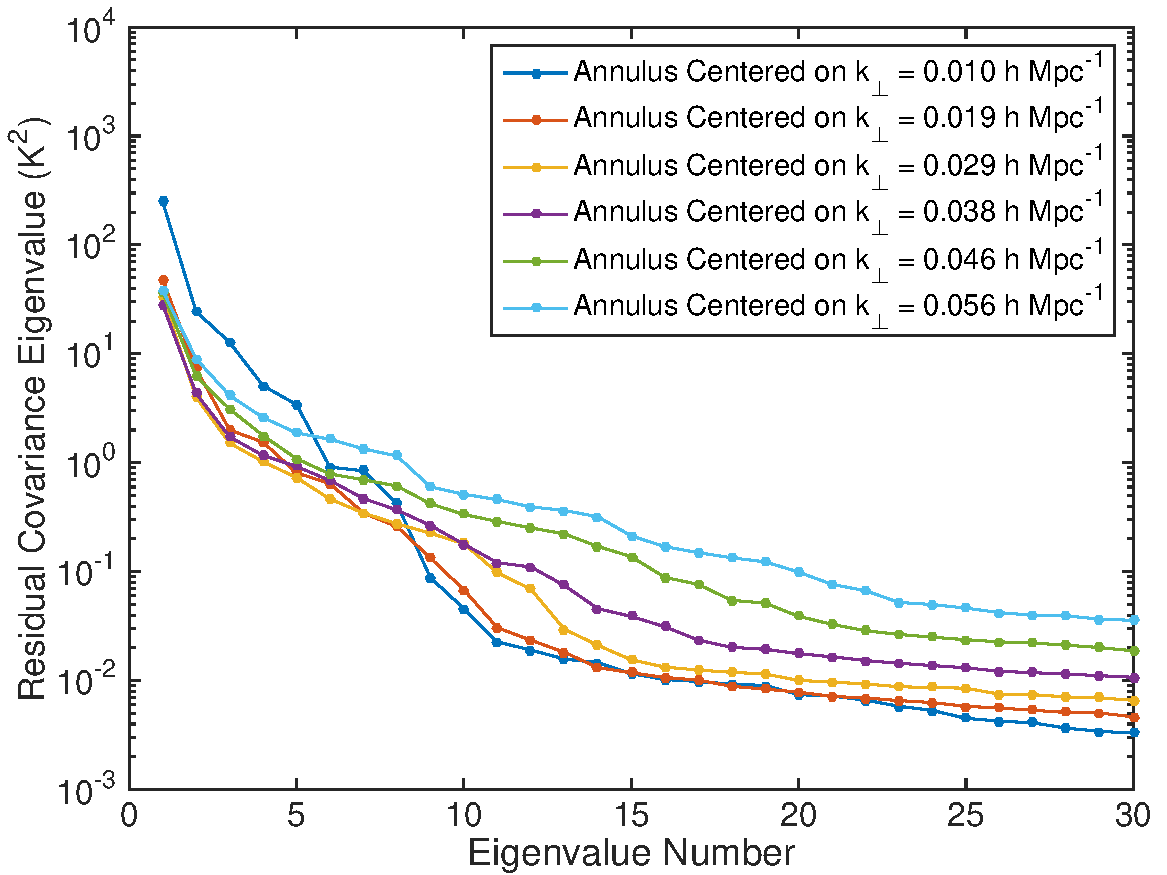
\includegraphics[width=.48\textwidth]{chap4_empirical_covariance/wedge_eigenvalues.pdf}
	\caption[Plot of the 30 largest eigenvalues of the observed residual foreground covariance matrix.]{The evolution of the wedge with $k_\perp$ motivates us to model foregrounds separately for discrete values of $k_\perp$. In this plot of the 30 largest eigenvalues of the observed residual covariance (which should include both noise and foregrounds) sampled in six concentric annuli, we see steeper declines toward a noise floor for the inner annuli than the outer annuli. This is consistent with the expected effect of the wedge---higher $k_\perp$ modes should be foreground contaminated at higher $k_\|$.}
	\label{fig:wedge_eigenvalues}
\end{figure}
 
Because we seek only to estimate the foreground portion of the covariance, the formal rank deficiency of $\CHat^\text{res}_{uv}$ is not a problem.\footnote{In fact, the rank of $\CHat^\text{res}_{uv}$ is $N_\text{LOS} - 3$ if $N^\text{LOS}-2 \le n_f$.} All we require is that the largest (and thus more foreground-dominated) modes be well measured. In this analysis, we used six concentric annuli to create six different frequency-frequency foreground covariances. Using more annuli allows for better modeling of the evolution of the wedge with $k_\perp$ at the expense of each estimate being more susceptible to noise and rank deficiency. 

%%%%%%%%%%%%%%%%%%%%%%%%%%%%%%%%%%%%%%%%%%%%%%%%%%%%%%%%%%%%%%%%%%%%%%%%%%

\subsubsection{Subtract the properly projected noise covariance.}
 
The covariances computed from these $uv$ lines of sight include contributions from the 21\,cm signal and instrumental noise as well as foregrounds. We can safely ignore the signal covariance for now as we are far from the regime where sample variance is significant. We already have a theoretically motivated model for the noise (based on the $uv$ sampling) that has been empirically rescaled to the observed noise in the difference of time-interleaved data (the same basic procedure as in \cite{X13}). We would like an empirical estimate of the residual foreground covariance alone to use in $\CC^{FG}$ and thus must subtract off the part of our measurement we think is due to noise variance.

To get to $\CHat^\text{FG}_{uv}$ from $\CHat^\text{res}_{uv}$, we subtract our best guess of the portion of $\CHat^\text{res}_{uv}$ that is due to noise, which we approximate by averaging the noise model variances in all the other $uv$ cells in the annulus at that given frequency, yielding
\beq
\widehat{C}_{uv,ff'}^\text{N} = \frac{1}{N^\text{LOS}} \hspace{-2mm}  \sum_{\substack{\text{other } u',v' \\ \text{in annulus}}}  \hspace{-2mm} \delta_{uu'} \delta_{vv'} \delta_{ff'} C^{N}_{uu'vv'ff'}.
\eeq
Note, however, that $\CHat_{uv}^\text{N}$ is full rank while $\CHat_{uv}^{res}$ is typically rank deficient. Thus a naive subtraction would oversubtract the noise variance in the part of the subspace of $\CHat_{uv}^\text{N}$ where $\CHat_{uv}^{res}$ is identically zero. Instead, the proper procedure is to find the projection matrices $\Proj_{uv}$ that discard all eigenmodes outside the subspace where $\CHat_{uv}^\text{res}$ is full rank. Each should have eigenvalues equal to zero or one only and have the property that
\beq
\Proj_{uv} \CHat_{uv}^\text{res} \Proj_{uv}^\trans = \CHat_{uv}^\text{res}.
\eeq
Only after projecting out the part of $\CHat^N_{uv}$ inside the unsampled subspace can we self-consistently subtract our best guess of the noise contribution to the subspace in which we seek to estimate foregrounds. In other words, we estimate $\CHat^\text{FG}_{uv}$ as
\beq
\CHat^\text{FG}_{uv} = \CHat_{uv}^\text{res} - \Proj_{uv} \CHat_{uv}^\text{N} \Proj_{uv}^\trans.
\eeq

We demonstrate the effectiveness of this technique in Figure \ref{fig:fourier_diags} by plotting the diagonal elements of the Fourier transform of $\CHat_{uv}^\text{res}$ and $\CHat_{uv}^\text{FG}$ along the line of sight. Subtracting of the noise covariance indeed eliminates the majority of the power in the noise dominated modes at high $k_\|$; thus we expect it also to fare well in the transition region near the edge of the wedge where foreground and noise contributions are comparable.

\begin{figure*}[]  
	\centering 
	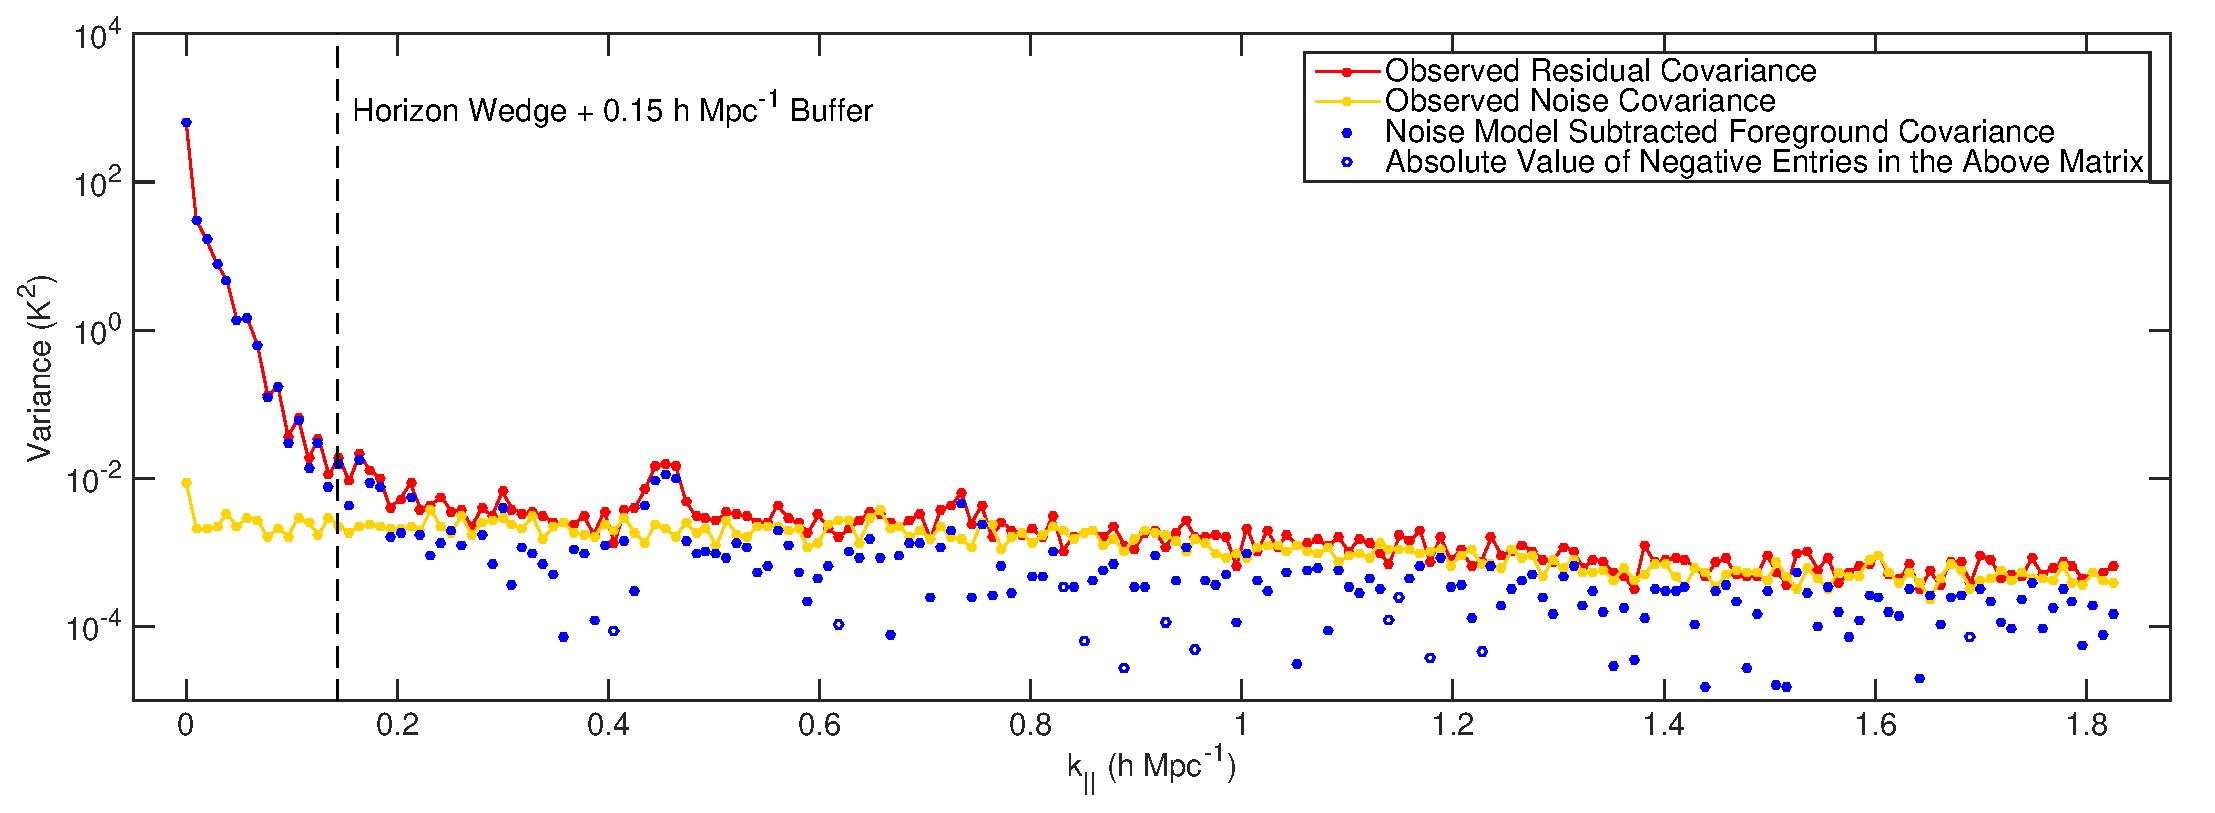
\includegraphics[width=1\textwidth]{chap4_empirical_covariance/fourier_diagonal.pdf}
	\caption[Examination of the diagonal elements of the observed residual and inferred foreground covariance matrices in Fourier space.]{Examining the diagonal elements of the observed residual and inferred foreground covariance matrices in Fourier space reveals the effectiveness of subtracting model for the noise covariance. In red, we plot the observed residual covariance, which contains both foregrounds and noise. As a function of $k_\|$, the two separate relatively cleanly---there is a steeply declining foreground portion on the left followed by a relatively flat noise floor on the right. The theory that the right-hand portion is dominated by noise is borne out by the fact that it so closely matches the observed noise covariance, inferred lines of sight of $\x_1 - \x_2$, which should have only noise and no sky signal at all. The regions where they differ significantly, for example at $k_\| \sim 0.45$\,$h$\,Mpc$^{-1}$ , are attributable to systematic effects like the MWA's coarse band structure that have not been perfectly calibrated out. For the example covariances shown here (which correspond to a mode in the annulus at $k_\perp \approx 0.010$\,$h$\,Mpc$^{-1}$), we can see that subtracting a properly projected noise covariance removes most of the power from the noise-dominated region, leaving only residual noise that appears both as negative power (open blue circle) and as positive power (closed blue circles) at considerably lower magnitude.}
	\label{fig:fourier_diags}
\end{figure*} 
 
%%%%%%%%%%%%%%%%%%%%%%%%%%%%%%%%%%%%%%%%%%%%%%%%%%%%%%%%%%%%%%%%%%%%%%%%%%

\subsubsection{Perform a $k_\|$ filter on the covariance.} \label{sec:filter}

Despite the relatively clean separation of foreground and noise eigenvalues, inspection of some of the foreground-dominated modes in the top panel of Figure \ref{fig:eigenvectors} reveals residual noise. Using a foreground covariance constructed from these noisy foreground eigenmodes to downweight the data during power spectrum estimation would errantly downweight some high $k_\|$ modes in addition to the low $k_\|$ foreground-dominated modes. To avoid this double counting of the noise, we allow the foreground covariance to include only certain $k_\|$ modes by filtering $\CHat^\text{FG}_{uv}$ in Fourier space to get $\CHat^\text{FG,filtered}_{uv}$. Put another way, we are imposing a prior on which Fourier modes we think have foreground power in them. The resulting noise filtered eigenmodes are shown in the bottom panel of Figure \ref{fig:eigenvectors}.

\begin{figure}[] 
	\centering 
	\includegraphics[width=.48\textwidth]{chap4_empirical_covariance/eigenvectors.pdf} 
	\caption[Results of fourier filtering the eigenmodes.]{The foreground covariance we estimate from our limited data set is still very noisy, and we run the risk of overfitting the noise in our measurements if we take it at face value. In the top panel, we plot the eigenvectors corresponding to the five largest eigenvalues of $\CHat^\text{FG}$ for a mode in the annulus centered on $k_\perp \approx 0.010$\,$h$\,Mpc$^{-1}$.  In the bottom panel, we show dominant eigenvectors of the Fourier-filtered covariance. As expected, they resemble the first five Fourier modes. The missing data every 1.28 MHz are due to channels flagged at the edge of the coarse bandpass of the MWA's polyphase filter bank---the most difficult part of the band to calibrate.} 
	\label{fig:eigenvectors}
\end{figure}   

In practice, implementing this filter is subtle. We interpolate $\CHat^\text{FG}$ over the flagged frequency channels using a cubic spline, then symmetrically pad the covariance matrix, forcing its boundary condition to be periodic. We then Fourier transform, filter, inverse Fourier transform, remove the padding, and then rezero the flagged channels. 

Selecting a filter to use is also a subtle choice. We first keep modes inside the horizon wedge with an added buffer. For each annulus, we calculate a mean value of $k_\perp$, and then use Equation \eqref{eq:wedge} to calculate the $k_\|$ value of the horizon wedge, using $\theta_0 = \pi/2$. Although the literature suggests a $0.1$ to $0.15$\,$h$\,Mpc$^{-1}$ buffer for ``suprahorizon emission'' due to some combination of intrinsic spectral structure of foregrounds, primary beam chromaticity, and finite bandwidth \cite{pober13,PoberNextGen}, we pick a conservative $0.5$\,$h$\,Mpc$^{-1}$. Then we examine the diagonal of $\CHat^\text{FG}$ (Figure \ref{fig:fourier_diags}) to identify additional foreground modes, this time in the EoR window, due to imperfect bandpass calibration appearing as spikes. One example is the peak at $k_\| \sim 0.45$\,$h$\,Mpc$^{-1}$. Such modes contribute errant power to the EoR window at constant $k_\|$. Since these modes result from the convolution of the foregrounds with our instrument, they also should be modeled in $\CC^{FG}$ in order to minimize their leakage into the rest of the EoR window. 

One might be concerned that cosmological signal and foregrounds theoretically both appear in the estimate of $\CC^{FG}$ that we have constructed, especially with our conservative $0.5$\,$h$\,Mpc$^{-1}$ buffer that allows foregrounds to be discovered well into the EoR window. For the purposes of calculating $\CC^{-1}(\widehat{\x}-\mean)$ in the quadratic estimator in Equation \eqref{eq:QuadEst}, that is fine since its effect is to partially relax the assumption that sample variance can be ignored. However, the calculation of the bias depends on being able to differentiate signal from contaminants \cite{Maxpowerspeclossless,LT11,DillonFast}. 

The noise contribution to the bias can be eliminated by cross-correlating maps made from interleaved time steps \cite{X13}. However, we cannot use our inferred $\CC^{FG}$ to subtract a foreground bias without signal loss. That said, we can still set an upper limit on the 21\,cm signal. By following the data and allowing the foreground covariance to have power inside the EoR window, we are minimizing the leakage of foregrounds into uncontaminated regions and we are accurately marking those regions as having high variance. As calibration and the control of systematic effects improves, we should be able to isolate foregrounds to outside the EoR window, impose a more aggressive Fourier filter on $\CC^{FG}$, and make a detection of the 21\,cm signal by employing foreground avoidance.

%%%%%%%%%%%%%%%%%%%%%%%%%%%%%%%%%%%%%%%%%%%%%%%%%%%%%%%%%%%%%%%%%%%%%%%%%%

\subsubsection{Cut out modes attributable to noise.}

After suppressing the noisiest modes with our Fourier filter, we must select a cutoff beyond which the foreground modes are irrecoverably buried under noise. We do this by inspecting the eigenspectrum of $\CHat^\text{FG,filtered}_{uv}$. The true $\CC^{FG}$, by definition, admits only positive eigenvalues (though some of them should be vanishingly small). 

By limiting the number of eigenvalues and eigenvectors we ultimately associate with foregrounds, we also limit the potential for signal loss by allowing a large portion of the free parameters to get absorbed into the contaminant model \cite{EricAdrianEmpiricalGlobalForegrounds,ali15}. When measuring the power spectrum inside the EoR window, we can be confident that signal loss is minimal compared to foreground bias and other errors.

We plot in Figure \ref{fig:cov_steps} the eigenspectra of $\CHat_{uv}^\text{res}$, $\CHat^\text{FG}_{uv}$, and $\CHat^\text{FG,filtered}_{uv}$, sorted by absolute value. There are two distinct regions---the sharply declining foreground-dominated region and a flatter region with many negative eigenvalues. We excise eigenvectors whose eigenvalues are smaller in absolute value than the most negative eigenvalue. This incurs a slight risk of retaining a few noise dominated modes, albeit strongly suppressed by our noise variance subtraction and our Fourier filtering. Finally we are able to construct the full covariance $\CHat$ using Equation \eqref{eq:blockdiag}.

\begin{figure}[]  
	\centering 
	\includegraphics[width=.48\textwidth]{chap4_empirical_covariance/eigenvalue_stages.pdf}
	\caption[The evolution of the eigenvalues of our estimated foreground covariance matrix for a mode in the annulus corresponding to $k_\perp \approx 0.010$\,$h$\,Mpc$^{-1}$.]{The evolution of the eigenvalues of our estimated foreground covariance matrix for a mode in the annulus corresponding to $k_\perp \approx 0.010$\,$h$\,Mpc$^{-1}$ at each of the first three stages of covariance estimation. First we calculate a sample covariance matrix from the residual data cubes (shown in red). Next we subtract our best guess as to the part of the diagonal of that matrix that originates from instrumental noise, leaving the blue dots (open circles are absolute values of negative eigenvalues). Then we filter out modes in Fourier space along the line of sight that we think should be noise dominated, leaving the black dots. Finally, we project out the eigenvectors associated with eigenvalues whose magnitude is smaller than the largest negative eigenvalue, since those are likely due to residual noise. What remains is our best guess at the foreground covariance in an annulus and incorporates as well as possible our prior beliefs about its structure.}
	\label{fig:cov_steps}
\end{figure}  

%%%%%%%%%%%%%%%%%%%%%%%%%%%%%%%%%%%%%%%%%%%%%%%%%%%%%%%%%%%%%%%%%%%%%%%%%%

\subsection{Review of Assumptions and Caveats} \label{sec:caveats}

Before proceeding to demonstrate the effectiveness of our empirical covariance modeling method, it is useful to review and summarize the assumptions made about mapmaking and covariance modeling. Some are inherited from the previous application of quadratic power spectrum estimation to the MWA \cite{X13}, while others are necessitated by our new, more faithful foreground covariance. Relaxing these assumptions in a computationally efficient manner remains a challenge we leave for future work.

\begin{enumerate}[i.]
\item We adopt the flat sky approximation as in \cite{DillonFast,X13}, allowing us to use the fast Fourier transform to quickly compute power spectra. The error incurred from this approximation on the power spectrum is expected to be smaller than 1\% \cite{X13}.

\item We assume the expectation value of our uniformly weighted map is the true sky (i.e., $\langle \widehat{\x} \rangle = \x^\text{true}$) when calculating $\CC,_\beta$ in Equation \ref{eq:QuadEst}, again following \cite{X13}. In general $\langle \widehat{\x} \rangle$ is related to $\x^\text{true}$ by $\PSF$, the matrix of point spread functions \cite{dillonmapmaking}. Here we effectively approximate the PSF as position independent. Relaxing this approximation necessitates the full mapmaking theory presented in \cite{dillonmapmaking} which has yet to be integrated into a power spectrum estimation pipeline. 

\item We approximate the foreground covariance as uncorrelated between different $uv$ cells (and thus block diagonal). At some level there likely are correlations in $uv$, though those along the line of sight are far stronger. It may be possible to attempt to calculate these correlations empirically, but it would be very difficult considering relative strength of line-of-sight correlations. It may also be possible to use a nonempirical model, though that has the potential to make the computational speedups of \cite{DillonFast} more difficult to attain.
 
\item We approximate the frequency-frequency foreground covariance as constant within each annulus, estimating our covariance for each $uv$ cell only from other cells in the same annulus. In principle, even if the foreground residuals were isotropic, there should be radial evolution within each annulus which we ignore for this analysis. 

\item The Fourier filter is a nontrivial data analysis choice balancing risk of noise double counting against that of insufficiently aggressive foreground downweighting.

\item In order to detect the 21\,cm signal, we assume that foregrounds can be avoided by working within the EoR window. Out of fear of losing signal, we make no effort to subtract a residual foreground bias from the window. This makes a detection inside the wedge impossible and it risks confusing foreground contamination in the window for a signal. Only analysis of the dependence of the measurement on $z$, $k$, $k_\|$, and $k_\perp$ can distinguish between systematics and the true signal. 

\end{enumerate}

%%%%%%%%%%%%%%%%%%%%%%%%%%%%%%%%%%%%%%%%%%%%%%%%%%%%%%%%%%%%%%%%%%%%%%%%%%

\section{Results} \label{sec:results}

We can now demonstrate the statistical techniques we have motivated and developed in Section \ref{sec:methods} on the problem of estimating power spectra from a 3\,h observation with the 128-antenna MWA. We begin with a discussion of the instrument and the observations in Section \ref{sec:observation}. In Section \ref{sec:processing} we detail the data processing from raw visibilities to calibrated maps from which we estimate both the foreground residual covariance matrix and the power spectrum. Finally, in Section \ref{sec:results} we present our results and discuss lessons learned looking toward a detection of the 21\,cm signal.

%%%%%%%%%%%%%%%%%%%%%%%%%%%%%%%%%%%%%%%%%%%%%%%%%%%%%%%%%%%%%%%%%%%%%%%%%%

\subsection{Observation Summary} \label{sec:observation}

The 128-antenna Murchison Widefield Array began deep EoR observations in mid-2013. We describe here the salient features of the array and refer to \cite{TingaySummary} for a more detailed description. The antennas are laid out over a region of radius 1.5\,km in a quasirandom, centrally concentrated distribution which achieves approximately complete $uv$ coverage at each frequency over several hours of rotation synthesis \cite{beardsley13}. Each antenna element is a phased array of 16 wideband dipole antennas whose phased sum forms a discretely steerable 25$^\circ$ beams (full width at half maximum) at 150\,MHz with frequency-dependent, percent level sidelobes \cite{neben15}. We repoint the beam to our field center on a 30\,min cadence to correct for earth rotation, effectively acquiring a series of drift scans over this field. 

We observe the MWA ``EOR0'' deep integration field, centered at R.A.(J2000) $= 0^\text{h}\,0^\text{m}\,0^\text{s}$ and decl.(J2000) $= -30^\circ\,0'\,0''$. It features a near-zenith position, a high Galactic latitude, minimal Galactic emission \cite{GSM}, and an absence of bright extended sources. This last property greatly facilitates calibration in comparison to the ``EOR2'' field---a field dominated by the slightly resolved radio galaxy Hydra A at its center---which was used by \cite{williamsimaging} and \cite{X13}. A nominal 3\,h set of EOR0 observations was selected during the first weeks of observing to use for refining and comparing data processing, imaging, and power spectra pipelines \cite{JacobsPipelines}. In this work, we use the ``high band,'' near-zenith subset of these observations with 30.72\,MHz of bandwidth and center frequency of 182\,MHz, recorded on Aug 23, 2013 between 16:47:28 and 19:56:32 UTC (22.712 and 1.872 hours LST). 

%%%%%%%%%%%%%%%%%%%%%%%%%%%%%%%%%%%%%%%%%%%%%%%%%%%%%%%%%%%%%%%%%%%%%%%%%%

\subsection{Calibration and Mapmaking Summary} \label{sec:processing}

Preliminary processing, including radio frequency interference (RFI) flagging followed by time and frequency averaging, was performed with the \texttt{COTTER} package \cite{AndreMWARFI} on raw correlator data. These data were collected at 40\,kHz resolution with an integration time of 0.5\,s, and averaged to 80\,kHz resolution with a 2\,s integration time to reduce the data volume. Additionally, 80\,kHz at the upper and lower edges of each of 24 coarse channels (each of width 1.28\,MHz) of the polyphase filter bank is flagged due to known aliasing.

As in \cite{X13}, we undertake snapshot-based processing in which each minute-scale integration is calibrated and imaged independently. Snapshots are combined only at the last step in forming a Stokes $I$ image cube, allowing us to properly align and weight them despite different primary beams due to sky rotation and periodic repointing. 
While sources are forward modeled for calibration and foreground subtraction using the full position dependent PSF (i.e., the synthesized beam), we continue to approximate it as position independent (and equal to that of a point source at the field center) during application of uniform weighting and computation of the noise covariance. 

We use the calibration, foreground modeling, and first stage image products produced by the Fast Holographic Deconvolution\footnote{For a theoretical discussion of the algorithm see \cite{fhd}. The code is available at \url{https://github.com/miguelfmorales/FHD}.} (FHD) pipeline as described by \cite{JacobsPipelines}. The calibration implemented in the FHD package is an adaptation of the fast algorithm presented by \cite{Salvini2014} with a baseline cutoff of $b>50\lambda$. In this data reduction, the point source catalogs discussed below are taken as the sky model for calibration.  Solutions are first obtained per antenna and per frequency before being constrained to linear phase slopes and quadratic amplitude functions after correcting for a median antenna-independent amplitude bandpass.  The foreground model used for subtraction includes models both of diffuse radio emission \cite{AdamDiffuse} and point sources. In detail, the point source catalog is the union of a deep MWA point source survey within $20^\circ$ of the field center \cite{PattiCatalog1}, the shallower but wider MWA commissioning point source survey \cite{MWACS}, and the Culgoora catalog \cite{Slee1995}. Note that calibration and foreground subtraction of off-zenith observations are complicated by Galactic emission picked up by primary beam sidelobes, and are active topics of investigation \cite{pober16,nithya15,nithya15b}. During these observations a single antenna was flagged due to known hardware problems, and 1--5 more were flagged for any given snapshot due to poor calibration solutions.

These calibration, foreground modeling, and imaging steps constitute notable improvements over \cite{X13}. In that work, the presence of the slightly resolved Hydra A in their EOR2 field likely limited calibration and subtraction fidelity as only a point source sky model was used. In contrast, the EOR0 field analyzed here lacks any such nearby radio sources. Our foreground model contains $\sim 2500$ point sources within the main lobe and several thousand more in the primary beam sidelobes in addition to the aforementioned diffuse map. A last improvement in the imaging is the more frequent interleaving of time steps for the cross power spectrum, which we performed at the integration scale (2\,s) as opposed to the snapshot scale (a few minutes). This ensures that both $\xhat_1$ and $\xhat_2$ have identical sky responses and thus allows us to accurately estimate the noise in the array from difference cubes. Assuming that the system temperature contains both an instrumental noise temperature and a frequency dependent sky noise temperature that scales as $\nu^{-2.55}$, the observed residual root-mean-square brightness temperature is consistent with $T_\text{sys}$ ranging from 450\,K at 167\,MHz to 310\,K at 198\,MHz, in line with expectations \cite{beardsley13}.

As discussed in \cite{JacobsPipelines} and \cite{HazeltonEppsilon}, FHD produces naturally weighted sky, foreground model, ``weights,'' and ``variances'' cubes, as well as beam-squared cubes. All are saved in image space using the HEALPix format \cite{HEALPIX} with $N_\text{side}=1024$. Note that these image cubes are crops of full-sky image cubes to a $16^\circ\times16^\circ$ square field of view, as discussed below. The sky, foreground model, and weights cubes are image space representations of the measured visibilities, model visibilities, and sampling function, respectively, all originally gridded in $uv$ space using the primary beam as the gridding kernel. The variances cube is similar to the weights cube, except the gridding kernel is the {\textit square} of the $uv$ space primary beam. It represents the proper quadrature summation of independent noise in different visibilities when they contribute to the same $uv$ cell, and will ultimately become our diagonal noise covariance model. The FHD cubes from all ninety-four 112\,s snapshots are optimally combined in this ``holographic'' frame in which the true sky is weighted by two factors of the primary beam, as in \cite{X13}.

We perform a series of steps to convert the image cube output of FHD into uniformly weighted Stokes $I$ cubes accompanied by appropriate $uv$ coverage information for our noise model. We first map these data cubes onto a rectilinear grid, invoking the flat sky approximation. We do this by rotating the (RA,Dec) HEALPix coordinates of the EOR0 field to the north pole (0$^\circ$,90$^\circ$), and then projecting and gridding onto the $xy$ plane with $0.2^\circ\times0.2^\circ$ resolution over a $16^\circ\times16^\circ$ square field of view. To reduce the data volume while maintaining cosmological sensitivity, we coarse grid to approximately $0.5^\circ$ resolution by Fourier transforming and cropping these cubes in the $uv$ plane at each frequency. We form a uniformly weighted Stokes I cube $I_{\text{uni}}(\vec{\theta})$ by first summing the XX and YY data cubes, resulting in a naturally weighted, holographic stokes I cube $I_{\text{nat},h}(\vec{\theta})  = I_{XX,h}(\vec{\theta})+I_{YY,h}(\vec{\theta})$. Then we divide out the holographic weights cube $W_h({\vec{\theta}})$ in $uv$ space, which applies uniform weighting and removes one image space factor of the beam, and lastly divide out the second beam factor $B(\vec{\theta})$: $I_{\text{uni}}(\vec{\theta}) = \mathcal{F}^{-1}[\mathcal{F}I_{\text{nat},h}(\vec{\theta})/\mathcal{F}W_h(\vec{\theta})]/B(\vec{\theta})$, where $\mathcal{F}$ represents a Fourier transform and $B(\vec{\theta}) = [B_{XX}^2(\vec{\theta})+B_{YY}^2(\vec{\theta})]^{1/2}$. Consistent treatment of the variances cube requires $uv$ space division of {\it two} factors of the weights cube followed by image space division of {\it two} factors of the beam.

Lastly, we frequency average from 80 kHz to 160 kHz, flagging a single 160 kHz channel the edge of each 1.28\,MHz coarse channel due to polyphase filter bank attenuation and aliasing, which make these channels difficult to reliably calibrate. Following \cite{X13}, we also flag poorly observed $uv$ cells and $uv$ cells whose observation times vary widely between frequencies. In all cases, we formally set the variance in flagged channels and $uv$ cells in $\CC^N$ to infinity and use the pseudoinverse to project out flagged modes \cite{X13}. 
 
%%%%%%%%%%%%%%%%%%%%%%%%%%%%%%%%%%%%%%%%%%%%%%%%%%%%%%%%%%%%%%%%%%%%%%%%%%
  
\subsection{Power Spectrum Results}
 
We can now present the results of our method applied to 3\,h of MWA-128T data. We first study cylindrically averaged, two-dimensional (2D) power spectra and their statistics, since they are useful for seeing the effects of foregrounds and systematic errors on the power spectrum. We form these power spectra with the full 30.72\,MHz instrument bandwidth to achieve maximal $k_\|$ resolution.

We begin with the 2D power spectrum itself (Figure \ref{fig:2dPk}) in which several important features can be observed.
\begin{figure}[] 
	\centering 
	\includegraphics[width=.48\textwidth]{chap4_empirical_covariance/2dPk.png}
	\caption[Power spectrum results, exhibiting typical EoR window structure with orders-of-magnitude suppression of foregrounds in the EoR window.]{Our power spectrum clearly exhibits the typical EoR window structure with orders-of-magnitude suppression of foregrounds in the EoR window. Here we plot our estimates for $|P(k_\perp,k_\|)|$ for the full instrumental bandwidth, equivalent to the range $z=6.2$ to $z=7.5$. Overplotted is the wedge from Equation \ref{eq:wedge} corresponding to the first null in the primary beam (dash-dotted line), the horizon (dashed line), and the horizon with a relatively aggressive \wedgeBuffer\,$h$\,Mpc$^-1$ buffer (solid curve). In addition to typical foreground structure, we also see the effect of noise at high and very low $k_\perp$ where baseline coverage is poor. We also clearly see a line of power at constant $k_\| \approx 0.45$\,$h$\,Mpc$^{-1}$, attributable to miscalibration of the instrument's bandpass and cable reflections \cite{HazeltonEppsilon}.}
	\label{fig:2dPk}
\end{figure}  
First, the wedge and EoR window are clearly distinguishable, with foregrounds suppressed by at least 5 orders of magnitude across most of the EoR window. At high $k_\perp$, the edge of the wedge is set by the horizon while at low $k_\perp$ the cutoff is less clear. There appears to be some level of suprahorizon emission, which was also observed with PAPER in \cite{pober13} and further explained by \cite{AdrianWedge1}. Consistent with Figure \ref{fig:wedge_eigenvalues} we see the strongest foreground residual power at low $k_\perp$, meaning that there still remains a very large contribution from diffuse emission from our Galaxy---potentially from sidelobes of the primary beam affecting the shortest baselines \cite{nithya15,nithya15b}.

We also see evidence for less-than-ideal behavior. Through we identified spectral structure appearing at $k_\| \sim 0.45$\,$h$\,Mpc$^{-1}$ in Figure \ref{fig:fourier_diags} and included it in our foreground residual covariance, that contamination still appears here as a horizontal line. By including it in the foreground residual model, we increase the variance we associate with those modes and we decrease the leakage out of those modes, isolating the effect to only a few $k_\|$ bins.

While Figure \ref{fig:2dPk} shows the magnitude of the 2D power spectrum, Figure \ref{fig:2dPkArcSinh} shows its sign using a split color scale, providing another way to assess foreground contamination in the EoR window. 
\begin{figure}[] 
	\centering 
	\includegraphics[width=.48\textwidth]{chap4_empirical_covariance/2dPkArcSinh.png}
	\caption[By using an estimator of the power spectrum with uncorrelated errors between bins, we can see that most of the EoR window is noise dominated.]{By using an estimator of the power spectrum with uncorrelated errors between bins, we can see that most of the EoR window is noise dominated in our power spectrum measurement. Here we show the inverse hyperbolic sine of the power spectrum, which behaves linearly near zero and logarithmically at large magnitudes. Because we are taking a cross power spectrum between two data cubes with uncorrelated noise, noise dominated regions are equally likely to have positive power as negative power. Since we do not attempt to subtract a foreground bias, foreground contaminated regions show up as strongly positive. That includes the wedge, the bandpass line at $k_\| \approx 0.45$\,$h$\,Mpc$^{-1}$  (see Figure \ref{fig:2dPk}), and some of the EoR window at low $k_\perp$ and relatively low $k_\|$, consistent with the suprahorizon emission seen in \cite{pober13}.}
	\label{fig:2dPkArcSinh}
\end{figure}  
Because we are taking the cross power spectrum between two cubes with identical sky signal but independent noise realizations, the noise dominated regions should be positive or negative with equal probability. This is made possible by our use of a power spectrum estimator normalized such that $\boldsymbol\Sigma \equiv \text{Cov}(\widehat{\p})$ is a diagonal matrix \cite{DillonFast}. This choice limits leakage of foreground residuals from the wedge into the EoR window \cite{X13}.

By this metric, the EoR window is observed to be noise dominated with only two notable exceptions. The first is the region just outside the wedge at low $k_\perp$ attributable to suprahorizon emission due to some combination of  intrinsic foreground spectral structure, beam chromaticity, and finite bandwidth. This suggests our aggressive 0.02\,$h$\,Mpc$^{-1}$ cut beyond the horizon will leave in some foreground contamination when we bin to form one-dimensional (1D) power spectra. As long as we are only claiming an upper limit on the power spectrum, this is fine. A detection of foregrounds is also an upper limit on the cosmological signal. More subtle is the line of positive power at $k_\| \sim 0.45$\,$h$\,Mpc$^{-1}$, confirming our hypothesis that the spike observed in Figure \ref{fig:2dPk} is indeed an instrumental systematic since it behaves the same way in both time-interleaved data cubes. There is also a hint of a similar effect at $k_\| \sim 0.75$\,$h$\,Mpc$^{-1}$, possibly visible in Figure \ref{fig:fourier_diags} as well. We attribute both to bandpass miscalibration due to cable reflections, complicated at these frequency scales by the imperfect channelization of the MWA's two-stage polyphase filter, as well as slight antenna dependence of the bandpass due to cable length variation \cite{HazeltonEppsilon}.

Additionally, the quadratic estimator formalism relates our covariance models of residual foregrounds and noise to the expected variance in each band power \cite{LT11,DillonFast,X13}, which we plot in Figure \ref{fig:2dError}.
\begin{figure}[] 
	\centering 
	\includegraphics[width=.48\textwidth]{chap4_empirical_covariance/2dError.png}
	\caption[Expected variance on each band power.]{By including both residual foregrounds and noise in $\CC$, our model for the covariance, we can calculate the expected variance on each band power in $\widehat{\p}$, which we show here. We see more variance at high (and also very low) $k_\perp$ where we have few baselines. We also see high variance at low $k_\|$ consistent with foregrounds. We see the strongest foregrounds at low $k_\perp$, which implies that the residual foregrounds have a very strong diffuse component that we have much to gain from better diffuse models to subtract. We also see that foreground-associated variance extends to higher $k_\|$ at high $k_\perp$, which is exactly the expected effect from the wedge. Both these observations are consistent with the structure of the eigenmodes we saw in Figure \ref{fig:wedge_eigenvalues}. Because we have chosen a normalization of $\widehat{\p}$ such that the $\text{Cov}(\widehat{\p})$ is diagonal, this is a complete description of our errors. Furthermore, it means that the band powers form a mutually exclusive and collectively exhaustive set of measurements.}
	\label{fig:2dError}
\end{figure}
As we have chosen our power spectrum normalization $\M$ such that $\boldsymbol\Sigma \equiv \text{Cov}(\widehat{\p})$ is diagonal, it is sufficient to plot the diagonal of $\boldsymbol\Sigma^{1/2}$, the standard deviation of each band power. The EoR window is seen clearly here as well. There is high variance at low and high $k_\perp$ where the $uv$ coverage is poor, and also in the wedge due to foreground residuals. It is particularly pronounced in the bottom left corner, which is dominated by residual diffuse foregrounds.

As our error covariance represents the error due to both noise and foregrounds we expect to make in an estimate of the 21\,cm signal, it is interesting to examine the ``signal to error ratio'' in Figure \ref{fig:2dSNR}---the ratio of Figure \ref{fig:2dPk} to Figure \ref{fig:2dError}.
\begin{figure}[] 
	\centering 
	\includegraphics[width=.48\textwidth]{chap4_empirical_covariance/2dSNR.png}
	\caption[The foreground wedge is clear in the ratio of our measured power spectrum to the modeled variance]{The foregrounds' wedge structure is particularly clear when looking at the ratio of our measured power spectrum to the modeled variance, shown here. Though the variance in foreground residual dominated parts of the $k_\perp$-$k_\|$ plane are elevated (see Figure \ref{fig:2dError}), we still expect regions with signal to error ratios greater than one. This is largely due to the fact that we choose not to subtract a foreground bias for fear of signal loss. This figure shows us most clearly where the foregrounds are important and, as with Figure \ref{fig:2dPkArcSinh}, it shows where we can hope to do better with more integration time and where we need better calibration and foreground modeling to further integrate down.}
	\label{fig:2dSNR}
\end{figure}
The ratio is of order unity in noise dominated regions---though it is slightly lower than what we might naively expect due to our conservative estimate of $\boldsymbol\Sigma$ \cite{X13}. That explains the number of modes with very small values in Figure \ref{fig:2dError}. In the wedge and just above it, however, the missubtracted foreground bias is clear, appearing as a high significance ``detection'' of the foreground wedge in the residual foregrounds. The bandpass miscalibration line at $k_\| \sim 0.45$\,$h$\,Mpc$^{-1}$ also appears clearly due to both foreground bias and possibly an underestimation of the errors. Hedging against this concern, we simply project out this line from our estimator that bins 2D power spectra into 1D power spectra by setting the variance of those bins to infinity.

Though useful for the careful evaluation of our techniques and of the instrument, the large bandwidth data cubes used to make Figures \ref{fig:2dPk} and \ref{fig:2dPkArcSinh} encompass long periods of cosmic time over which the 21\,cm power spectrum is expected to evolve. The cutoff is usually taken to be $\Delta z \lesssim 0.5$ \cite{mao08}. These large data cubes also violate the assumption in \cite{DillonFast} that channels of equal width in frequency correspond to equal comoving distances, justifying the use of the fast Fourier transform. Therefore, we break the full bandwidth into three 10.24\,MHz segments before forming spherically averaged power spectra, and estimate the foreground residual covariance and power spectrum independently from each. We bin our 2D power spectra into 1D power spectra using the optimal estimator formalism of \cite{X13}. In our case, since we have chosen $\M$ such that $\boldsymbol\Sigma$ is diagonal, this reduces to simple inverse variance weighting with the variance on modes outside the EoR window or in the $k_\| \sim 0.45$\,$h$\,Mpc$^{-1}$ line set to infinity.

In Figure \ref{fig:1dDeltaSq} we show the result of that calculation as a ``dimensionless'' power spectra $\Delta^2(k) \equiv k^3 P(k) /2\pi^2$.
\begin{figure*}[] 
	\centering 
	\includegraphics[width=1\textwidth]{chap4_empirical_covariance/1dDeltaSqMultiRedshift.pdf}
	\caption[Limits on the 21\,cm power spectrum at three redshifts.]{Finally, we can set confident limits on the 21\,cm power spectrum at three redshifts by splitting our simultaneous bandwidth into three 10.24\,MHz data cubes. The lowest $k$ bins show the strongest ``detections,'' though they are attributable to suprahorizon emission \cite{pober13} that we expect to appear because we only cut out the wedge and a small buffer (0.02\,$h$\,Mpc$^{-1}$) past it. We also see marginal ``detections'' at higher $k$ which are likely due to subtle bandpass calibration effects like cable reflections. The largest such error, which occurs at bins around $k_\| \sim 0.45$\,$h$\,Mpc$^{-1}$ and can be seen most clearly in Figure \ref{fig:2dSNR}, has been flagged and removed from all three of these plots. Our absolute lowest limit requires $\Delta^2(k) < \limitDeltaSq$\,mK$^2$ at 95\% confidence at comoving scale $k = \limitk$\,$h$\,Mpc$^{-1}$ and $z = \limitz$, which is consistent with published limits \cite{gmrtsignalloss,X13,parsons14,DannyMultiRedshift,ali15}. We also include a simplistic thermal noise calculation (dashed line), based on our observed system temperature. Though it is not directly comparable to our measurements, since it has different window functions, it does show that most of our measurements are consistent with thermal noise. For comparison, we also show the theoretical model of \cite{BarkanaPS2009} (which predicts that reionization ends before $z=6.4$) at the central redshift of each bin. While we are still orders of magnitude away from the fiducial model, recall that the noise in the power spectrum scales inversely with the integration time, not the square root.}
	\label{fig:1dDeltaSq}
\end{figure*}
We choose our binning such that the window functions (calculated as in \cite{X13} from our covariance model) were slightly overlapping. 

Our results are largely consistent with noise. Since noise is independent of $k_\|$ and $k\approx k_\|$ for most modes we measure, the noise in $\Delta^2(k)$ scales as $k^3$. We see deviations from that trend at low $k$ where modes are dominated by residual foreground emission beyond the horizon wedge and thus show elevated variance and bias in comparison to modes at higher $k$. Since we do not subtract a bias, even these ``detections'' are upper limits on the cosmological signal.

A number of barely significant ``detections'' are observed at higher $k$. Though we excise bins associated with the $k_\| \sim 0.45$\,$h$\,Mpc$^{-1}$ line, the slight detections may be due to leakage from that line. At higher $z$, the feature may due to reflections from cables of a different length, though some may be plausibly attributable to noise. Deeper integration is required to investigate further. 

Our best upper limit at 95\% confidence is $\Delta^2(k) < \limitDeltaSq$\,mK$^2$ at $k = \limitk$\,$h$\,Mpc$^{-1}$ around $z = \limitz$. Our absolute lowest limit is about 2 times lower than the best limit in \cite{X13}, though the latter was obtained at substantially higher redshift and lower $k$, making the two somewhat incomparable. Our best limit is roughly 3 orders of magnitude better than the best limit of \cite{X13} over the same redshift range, and the overall noise level (as measured by the part of the power spectrum that scales as $k^3$) is more than 2 orders of magnitude smaller. This cannot be explained by more antenna tiles alone; it is likely that the noise level was overestimated in \cite{X13} due to insufficiently rapid time interleaving of the data cubes used to infer the overall noise level.

Although one cannot directly compare limits at different values of $k$ and $z$, our limit is similar to the GMRT limit \cite{gmrtsignalloss}, $6.2\times 10^4$\,mK$^2$ at $k = 0.50$\,$h$\,Mpc$^{-1}$ and $z=8.6$ with 40\,h of observation, and remains higher than the best PAPER limit \cite{PAPER64Limits} of 502\,mK$^2$ between $k = 0.15$\,$h$\,Mpc$^{-1}$ and $k=0.50$\,$h$\,Mpc$^{-1}$ and $z=8.4$ with 4.5 months of observation.
 
In Figure \ref{fig:1dDeltaSq} we also plot a theoretical model from \cite{BarkanaPS2009} predicting that reionization has ended by the lowest redshift bin we measure. We remain more than 3 orders of magnitude (in mK$^2$) from being able to detect that particular reionization model, naively indicating that roughly 3000\,h of data are required for its detection. This appears much larger than what previous sensitivity estimates have predicted for the MWA (e.g.~\cite{beardsley13}) in the case of idealized foreground subtraction. 
 
However, much of this variance is due to the residual foregrounds and systematics in the EoR window identified by our empirical covariance modeling method, not thermal noise (see Figure \ref{fig:2dError}). More integration will not improve those modes unless it allows for a better understanding of our instrument, better calibration, and better foreground models---especially of diffuse emission which might contaminate the highly sensitive bottom left corner of the EoR window. Eliminating this apparent ``suprahorizon'' emission, seen most clearly as detections in Figure \ref{fig:2dSNR} below $k \approx 0.2$\,$h$\,Mpc$^{-1}$, is essential to achieving the forecast sensitivity of the MWA \cite{beardsley13}. If we can do so, we may still be able to detect the EoR with 1000\,h or fewer. This is especially true if we can improve the subtraction of foregrounds to the point where we can work within the wedge, which can vastly increase the sensitivity of the instrument \cite{beardsley13,PoberNextGen}. On the other hand, more data may reveal more systematics lurking beneath the noise which could further diminish our sensitivity.

%%%%%%%%%%%%%%%%%%%%%%%%%%%%%%%%%%%%%%%%%%%%%%%%%%%%%%%%%%%%%%%%%%%%%%%%%%

\section{Summary and Future Directions} \label{sec:summary}

In this work, we developed and demonstrated a method for empirically deriving the covariance of residual foreground contamination, $\CC^{FG}$, in observations designed to measure the 21\,cm cosmological signal. Understanding the statistics of residual foregrounds allows us to use the quadratic estimator formalism to quantify the error associated with missubtracted foregrounds and their leakage into the rest of the EoR window. Because of the complicated interaction between the instrument and the foregrounds, we know that the residual foregrounds will have complicated spectral structure, especially if the instrument is not perfectly calibrated. By deriving our model for $\CC^{FG}$ empirically, we could capture those effects faithfully and thus mitigate the effects of foregrounds in our measurement (subject to certain caveats which we recounted in Section \ref{sec:caveats}).

Our strategy originated from the assumption that the frequency-frequency covariance, modeled as a function of $|u|$, is the most important component of the foreground residual covariance. We therefore used sample covariances taken in annuli in Fourier space as the starting point of our covariance model. These models were adjusted to avoid double counting the noise variance and filtered in Fourier space to minimize the effect of noise in the empirically estimated covariances. Put another way, we combined our prior beliefs about the structure of the residual foregrounds with their observed statistics in order to build our models.

We demonstrated this strategy through the power spectrum analysis of a 3\,h preliminary MWA data set. We saw the expected wedge structure in both our power spectra and our variances. We saw that most of the EoR window was consistent with noise, and we understand why residual foregrounds and systematics affect the regions that they do. We were also able to set new MWA limits on the 21\,cm power spectrum from $z=6.2$ to $7.5$, with an absolute best 95\% confidence limit of $\Delta^2(k) < \limitDeltaSq$\,mK$^2$ at $k = \limitk$\,$h$\,Mpc$^{-1}$ and $z = \limitz$, consistent with published limits \cite{parsons14,DannyMultiRedshift}.

This work suggests a number of avenues for future research. Of course, improved calibration and mapmaking fidelity---especially better maps of diffuse Galactic structure---will improve power spectrum estimates and and allow deeper integrations without running up against foregrounds or systematics. Relaxing some of the mapmaking and power spectrum assumptions discussed in Section \ref{sec:caveats} may further mitigate these effects. A starting point is to integrate the mapmaking and statistical techniques of \cite{mapmaking} with the fast algorithms of \cite{DillonFast}. The present work is based on the idea that it is simpler to estimate $\CC^{FG}$ from the data than from models of the instrument and the foregrounds. But if we can eliminate systematics to the point where we really understand $\PSF$, the relationship between the true sky and our dirty maps, then perhaps we can refocus our residual foreground covariance modeling effort on the statistics of the true sky residuals using the fact that $\CC^{FG} = \PSF \CC^{FG,\text{true}} \PSF^\trans.$ Obtaining such a complete understanding of the instrument will be challenging, but it may be the most rigorous way to quantify the errors introduced by missubtracted foregrounds and thus to confidently detect the 21\,cm power spectrum from the epoch of reionization.

\section{Acknowledgements}

We would like to thank Adrian Liu, Aaron Parsons, and Jeff Zheng for helpful discussions. We also acknowledge an anonymous referee whose insightful questions led to the refinement of method in order to a bias that occurs when a $uv$ cell is used to estimate its own covariance and the ultimate form of Equation \ref{eq:CovEstOtherAnnuli}. We would also like to thank Rennan Barkana for the theoretical power spectra in Figure \ref{fig:1dDeltaSq}. This work was supported by NSF Grants AST-0457585, AST-0821321, AST-1105835, AST-1410719, AST-1410484, AST-1411622, and AST-1440343, by the MIT School of Science, by the Marble Astrophysics Fund, and by generous donations from Jonathan Rothberg and an anonymous donor. D.C.J. would like to acknowledge NSF support under AST-1401708.

This scientific work makes use of the Murchison Radio-astronomy Observatory, operated by CSIRO. We acknowledge the Wajarri Yamatji people as the traditional owners of the Observatory site. Support for the MWA comes from the U.S. National Science Foundation (grants AST-0457585, PHY-0835713, CAREER-0847753, and AST-0908884), the Australian Research Council (LIEF grants LE0775621 and LE0882938), the U.S. Air Force Office of Scientific Research (grant FA9550-0510247), and the Centre for All-sky Astrophysics (an Australian Research Council Centre of Excellence funded by grant CE110001020). Support is also provided by the Smithsonian Astrophysical Observatory, the MIT School of Science, the Raman Research Institute, the Australian National University, and the Victoria University of Wellington (via grant MED-E1799 from the New Zealand Ministry of Economic Development and an IBM Shared University Research Grant). The Australian Federal government provides additional support via the Commonwealth Scientific and Industrial Research Organisation (CSIRO), National Collaborative Research Infrastructure Strategy, Education Investment Fund, and the Australia India Strategic Research Fund, and Astronomy Australia Limited, under contract to Curtin University. We acknowledge the iVEC Petabyte Data Store, the Initiative in Innovative Computing and the CUDA Center for Excellence sponsored by NVIDIA at Harvard University, and the International Centre for Radio Astronomy Research (ICRAR), a Joint Venture of Curtin University and The University of Western Australia, funded by the Western Australian State government.



\chapter{Foreground and sensitivity analysis for 21cm/Infrared intensity mapping correlation studies from the Epoch of Reionization}

abstract

\section{Introduction}

\section{Power spectra of residual foreground}
\subsection{Power spectrum conventions}
\subsection{21\,cm foreground power spectra}
\subsection{IR foreground power spectra}

\section{Sensitivity and Experimental Design Study}
\subsection{Cross spectrum vs coherence}
\subsection{Sensitivity framework}

\section{Cross spectrum results}

\section{Discussion}


\chapter{Conclusion}

something here
\appendix 

\chapter{Review of noise in radio interferometers}
\label{chap:noisereview}

We review in this section the nature of signal and noise in radio interferometry in order to quantitatively understand nature of sky noise and self noise within a unified framework. Our discussion draws on \citet{thompsonmoranswenson, dewey94, kulkarni89,ellingson2011,synthesisimaging}, and aims to clarify the nature of nature of noise in current instruments.

\section{The Radio Sky and Radio Interferometry}
\label{sec:theradiosky}

The radio sky is an angularly and temporally incoherent radiation field\footnote{This description neglects coherent sources such as pulsars or masers which require different noise considerations, but are not of interest in 21\,cm observations.}. In practice, we consider it a continuum of uncorrelated, temporally incoherent point sources which fill the sky with some resolution. For analytic calculation we may assume this resolution to be infinite, while for numerical calculations the resolution will be determined by the length of the longest baseline. 

Let us introduce a real interferometer and consider how it receives such sky emission. Consider an FX correlator\footnote{In an FX correlator, the timestream from each antenna is Fourier transformed (F) first, and then multiplied (X) with those of other antennas.} which forms cross-correlations (known in radio interferometry as \textit{visibilities}) by first sampling the voltage $v_i(t)$ across antenna $i$ at sample frequency $f_s$ over the time period $\Delta T$. Each timestream is Fourier transformed to construct amplitudes $v_i(T,f)$ with frequency resolution $\Delta f=1/\Delta T$ during time window $T=0,\Delta T, 2\Delta T, ...$. The Fourier amplitudes are then cross multiplied with those of other antennas and time-averaged to form the visibility $V_{ij}(f)$,

\begin{equation}
\label{eqn:visdef}
V_{ij}(f)=\frac{1}{N_T}\sum_{T}v_i(T,f)v_j^*(T,f)
\end{equation}
where $N_T=t_\text{obs}\Delta f$ is the total number of measurements of each Fourier mode, $\Delta f$ is the channel bandwidth, and $t_\text{obs}$ is the total integration time.
The temporal coherence of each Fourier component is $1/\Delta f=\Delta T$, and thus samples of $v_i(T,f)$ at successive times are essentially independent\footnote{This constructive model of a radio interferometer is an alternate picture to the quasi-monochromatic plane wave approximation of \citet{synthesisimaging}.}. \textit{This means that we may consider the sky as a continuum of point sources emitting Fourier amplitudes with frequency spacing $\Delta f$, which vary randomly every time $\Delta T$.} 

Having quantified the operation of the FX correlator, we will express the visibility as a function of the sky intensity distribution $I(\theta,\phi)$ and evaluate its mean and variance. We first express the voltage Fourier amplitude across antenna $i$ during time window $T$ as an integral over the electric field Fourier amplitudes $E_0(T,\theta,\phi,f)$ of the continuum of point sources on the sky. These amplitudes are random numbers drawn every $\Delta T$ from a complex Gaussian distribution with variance equal\footnote{In fact, the electric field variance is equal to the intensity only up to a constant of proportionality which in the real world would be absorbed in calibration anyway, we thus neglect it here.} to $I(\theta,\phi)$. Summing over this continuum of sky sources, adding phases accounting for the antenna position on the ground, and adding the receiver noise $n_i(T,f)$, we find
\begin{equation}
\label{eqn:antvoltage}
v_i(T,f) = g\int E_0(\theta,\phi,f)e^{-i\vec{k}\cdot \vec{x}_i}d\Omega+n_i(T,f)
\end{equation}
where $g$ converts from incident electric field in the instrument polarization to voltage and $\vec{k}=\vec{k}(\theta,\phi,f)$. The measured visibility output by the correlator is specified by Eqns. \ref{eqn:visdef} and \ref{eqn:antvoltage}. The mean is given by the ensemble average of $V_{ij}(f)$,
\begin{eqnarray}
\langle V_{ij}(f)\rangle &=&\int\int \langle E_0(\theta,\phi,T,f)E_0^*(\theta',\phi',T,f)\rangle e^{-i(\vec{k}\cdot\vec{x}_i-\vec{k}'\cdot\vec{x}_j)}d\Omega \nonumber \\ 
&&+\delta_{ij}\sigma_\text{rec}^2
\end{eqnarray}
where $\sigma_\text{rec}^2\equiv\langle |n_i|^2\rangle$. Given that emission from different directions in uncorrelated, this reduces to 
\begin{eqnarray}
\label{eqn:vismean}
\langle V_{ij}(f)\rangle &=&\int\langle |E_0(\theta,\phi,T,f)|^2\rangle e^{-i\vec{k}\cdot(\vec{x}_i-\cdot\vec{x}_j)}d\Omega+\delta_{ij}\sigma_\text{rec}^2 \\
&=&\int I(\theta,\phi,f) e^{-i\vec{k}\cdot(\vec{x}_i-\cdot\vec{x}_j)}d\Omega+\delta_{ij}\sigma_\text{rec}^2 
\end{eqnarray}
This integral reduces to a Fourier transform over small fields of view (the van Cittert-Zernicke Theorem), demonstrating that the visibility mean is equal to the Fourier mode of the sky intensity distribution at angular scale $\lambda/|\vec{x}_i-\vec{x}_j|$, with autocorrelation ($i=j$) measurements incurring a receiver noise bias.

Let us now evaluate the variance of the visibility, defined as
\begin{equation}
\sigma_V^2(f)\equiv\langle |V_{ij}(f)|^2\rangle-|\langle V_{ij}(f)\rangle|^2
\end{equation}
where $\langle\rangle$ indicates an ensemble average, in practice equal to a time average over time windows $T$.
Substituting Eqns. \ref{eqn:visdef} and \ref{eqn:antvoltage} into this definition gives
\begin{eqnarray}
\sigma_V^2(f) &=&\frac{1}{N_T^2}\sum_{T,T'}\langle v_i(T,f)v_j^*(T,f)v_i^*(T',f)v_j(T',f)\rangle \nonumber \\
&-&\frac{1}{N_T^2}\sum_{T,T'}\langle v_i(T,f)v_j^*(T,f)\rangle \langle v_i^*(T',f)v_j(T',f)\rangle
\end{eqnarray}

Expanding the 4-product using Wick's theorem gives
\begin{eqnarray}
\sigma_V^2(f)&&=\frac{1}{N_T^2}\sum_{T,T'}[\langle v_i(T,f)v_j^*(T,f)\rangle\langle v_i^*(T',f)v_j(T',f)\rangle \nonumber \\
&&\hspace{18mm}+\langle v_i(T,f)v_i^*(T',f)\rangle\langle v_j^*(T,f)v_j(T',f)\rangle]\nonumber \\
&&-\frac{1}{N_T^2}\sum_{T,T'}\langle v_i(T,f)v_j^*(T,f)\rangle \langle v_i^*(T',f)v_j(T',f)\rangle
\end{eqnarray}
The first term cancels the last term in the equation, and the variance simplifies to
\begin{equation}
\label{eqn:varauto}
\sigma_V^2(f)=\frac{|\langle V_{ii}(f)\rangle|^2}{N_T}
\end{equation}
In summary, the visibility mean and variance are given by
\begin{eqnarray}
\langle V_{i\ne j}(f)\rangle &=&\int I(\theta,\phi,f)e^{-i\vec{k}\cdot(\vec{x}_i-\cdot\vec{x}_j)}d\Omega \label{eqn:vismean}\\
\sigma_V^2(f)&=&\frac{(\sigma^2_\text{sky}(f)+\sigma^2_\text{rec}(f))^2}{N_T} \label{eqn:visvar}
\end{eqnarray}
where $\sigma^2_\text{sky}\equiv\int I(\theta,\phi,f)d\Omega$ is the total received sky power. In the next subsections we will look at the limiting cases of these equations and define the different noise regimes in radio interferometry.

\section{Sky Noise, Self Noise, and Receiver Noise}
\label{sec:skyselfreceivernoise}
The receiver contribution to the variance ($\sigma_\text{rec}^2$) is known as \textit{receiver noise}, and typically dominates at high frequencies as the galactic synchrotron and bremsstrahlung brightness decreases rapidly with frequency. Neglecting real world complications such as cross-talk, receiver noise is uncorrelated between antennas, and can thus be mitigated by adding more antennas.

On the other hand, the contribution to the variance from sky emission ($\sigma_\text{sky}^2)$ is known as \textit{sky noise}. Why is this distinction useful? If the interferometer is sky noise dominated, then we are liberated from needing extremely low noise amplifiers or a very high fidelity impedance match with the sky as we would need in receiver noise dominated instruments. As sky noise results from actual sky emission and not electronics noise, it is not immediately clear whether it is entirely uncorrelated between different antennas, and thus, whether adding antennas improves sensitivity. To determine this, we must consider a last type of noise known as \textit{self noise}. 

The contribution of any sky emission to the visibility variance is known as \text{self noise} if that same emission contributes significantly to the visibility mean (Eqn. \ref{eqn:vismean}). Of course, \textit{any} source of sky emission contributes at \textit{some} level to both the visibility mean and variance, but the notion of sky noise is useful when it contributes a significant fraction of both. Physically this means that the voltage fluctuations across each antenna are dominated by the real emitted signal from the celestial source dominating the visibilities. But if that is the case then why is there any noise whatsoever in the visibility measurement? It is easy to understand the reason in the context of single dish measurements. Because the source emission is fundamentally stochastic, its emitted amplitude is a random timestream whose mean equals the true intensity only after infinitely many samples. Self noise may thus be regarded as the \textit{sample variance} on the measured visibilities. 

In a self noise dominated interferometer, adding more antennas provides little new information about the sky as they receive the same (albeit timeshifted) timestream of emission from each celestial source. Adding new antennas of course yields more baselines, but if these new visibilities provide little new information, then their noise must be correlated with those of existing baselines. To quantify this, we compute the covariance $C_{ij,kl}$ between baselines $ij$ and $kl$, defined by
\begin{equation}
C_{ij,kl}\equiv\langle V_{ij}V_{kl}^*\rangle-\langle V_{ij}\rangle\langle V_{kl}^*\rangle
\end{equation}
Evaluating this in the same way we calculate $\sigma_V^2$ in Sec. \ref{sec:theradiosky} results in
\begin{equation}
\label{eqn:covfinal}
C_{ij,kl}=\frac{\langle V_{ik}\rangle\langle V_{jl}^*\rangle}{N_T}
\end{equation}
We see that the covariance between baselines $ij$ and $kl$ is related to the visibilities which would be measured by baselines $ik$ and $jl$. The covariance increases if the distance between these baselines is reduced, or decreased if the distance increases, but it is independent of the length of the baselines themselves.

\begin{figure}[t]
\centering
\includegraphics[width=2.5in]{skynoise/array2by2.pdf}
\caption[The level of self noise in baselines is set by their separation.]{The level of self noise in baselines $ij$ and $kl$ is set not by the length of these baselines $d_{ij}$, but by the separation of these baselines from each other $d_{ik}$. }
\label{fig:array2by2}
\end{figure}

This result was first derived by \citet{kulkarni89} for the case of an extremely bright point source which dominates over all other sky emission and receiver noise. In that case, the noise correlation, defined as the ratio of covariance to variance, 
\begin{equation}
\label{eqn:noisecorr}
c \equiv \frac{C_{ij,kl}}{\sigma_V^2}=\frac{|\langle V_{ik}\rangle\langle V_{jl}^*\rangle|}{|\langle V_{ii}\rangle|^2}
\end{equation}
approaches unity, $c=|I_\text{source}e^{-i\vec{k}\cdot(\vec{x}_i-\vec{x}_k)}||I_\text{source}e^{i\vec{k}\cdot(\vec{x}_j-\vec{x}_l)}|/I_\text{source}^2=1$. 
This confirms our intuition that in the self noise regime the noise on different visibilities is strongly correlated, so adding additional antennas does not improve sensitivity. 

Lastly, let us consider the sky noise regime when it is \textit{not} self noise, as is the case in typical low frequency radio interferometers like the MWA. At MWA frequencies (100--200\,MHz), typical sources range from hundreds of mJy to several Jy, whereas the diffuse Galactic emission (dominated by radio synchrotron) has brightness temperature of $\sim200$\,K, translating into a flux density of $2 k_B T_\text{gal}\Omega_\text{FWHM}/\lambda^2\sim2 k_B T_\text{gal}/A\sim30$\,kJy. The noise power sourced by the receiver noise corresponds to an effective brightness temperature of 25--50\,K, subdominant to sky emission. Thus we see that the diffuse Galactic emission dominates the incident power, and thus, the visibility variance. Expressing the flux as a brightness temperature we arrive at the well-known radiometer equation.
\begin{equation}
\sigma_V=\frac{2 k_B T_\text{gal}}{A\sqrt{t_\text{obs}B}}
\end{equation}
But while the diffuse Galactic emission dominates the incident flux, and thus, the visibility variance, its contribution to the mean visibilities is very small. As discussed above, in the flat sky approximation, each visibility measures exactly one mode of the Fourier transform of the sky intensity distribution. The contribution of a constant background to non-zero Fourier modes is thus zero, meaning that the diffuse emission produces no self noise. 

In reality, the diffuse emission is not exactly constant across the sky and the curved sky disturbs the exact Fourier relationship so that even a constant sky background has some leakage into the visibility means. This real diffuse emission will result in some small level of self noise. To quantify this, consider the self-noise induced noise correlation between two parallel baselines positioned as close as possible from each other as in Fig. \ref{fig:array2by2} with $d_{12}=d_{13}=5\,\text{m}$, the size of an MWA tile. Assuming such short baselines are dominated by diffuse emission, the visibility mean is given by $\langle V_{ik}\rangle\sim(2k_BT_\text{gal}/\lambda^2)\int B(\theta,\phi)e^{i\vec{k}\cdot\vec{b}}d\Omega$. The integral is of order $10^{-1.5}$ or smaller over the MWA band, 100--200\,MHz, while $\langle V_{ii}\rangle \sim 2k_BT_\text{gal}/\lambda^2$. Then the noise correlation between the pair of baselines is $c\sim10^{-3}$ at worst. What does a noise correlation of 0.1\% mean? It means that the variance on the average of these two redundant baselines is 0.1\% larger than it would be were their noises independent, an entirely negligible effect. Note that this correlation does not affect how visibility noise averages down with time.

We find a comparable level of noise correlation, 0.1\%, for HERA dishes over the same band, and somewhat larger values of a few percent for PAPER near 100\,MHz. These numbers are worst cases, for physically touching baselines. In real arrays, even the closest antennas are typically placed no closer than of order a wavelength to mitigate cross-coupling, and of course a baseline has very few close neighbor baselines anyway, most other baselines are much farther away. 

%HERA is compact but has negligible sky noise correlation, but maybe that's because it's not electrically compact...should I use ultracompact instead???
%% This defines the bibliography file (main.bib) and the bibliography style.
%% If you want to create a bibliography file by hand, change the contents of
%% this file to a `thebibliography' environment.  For more information 
%% see section 4.3 of the LaTeX manual.
\begin{singlespace}
\bibliography{main}
%\bibliographystyle{plainnat}
\bibliographystyle{apj}
\end{singlespace}

\end{document}

